\documentclass{math_library}

%delete

\begin{document}
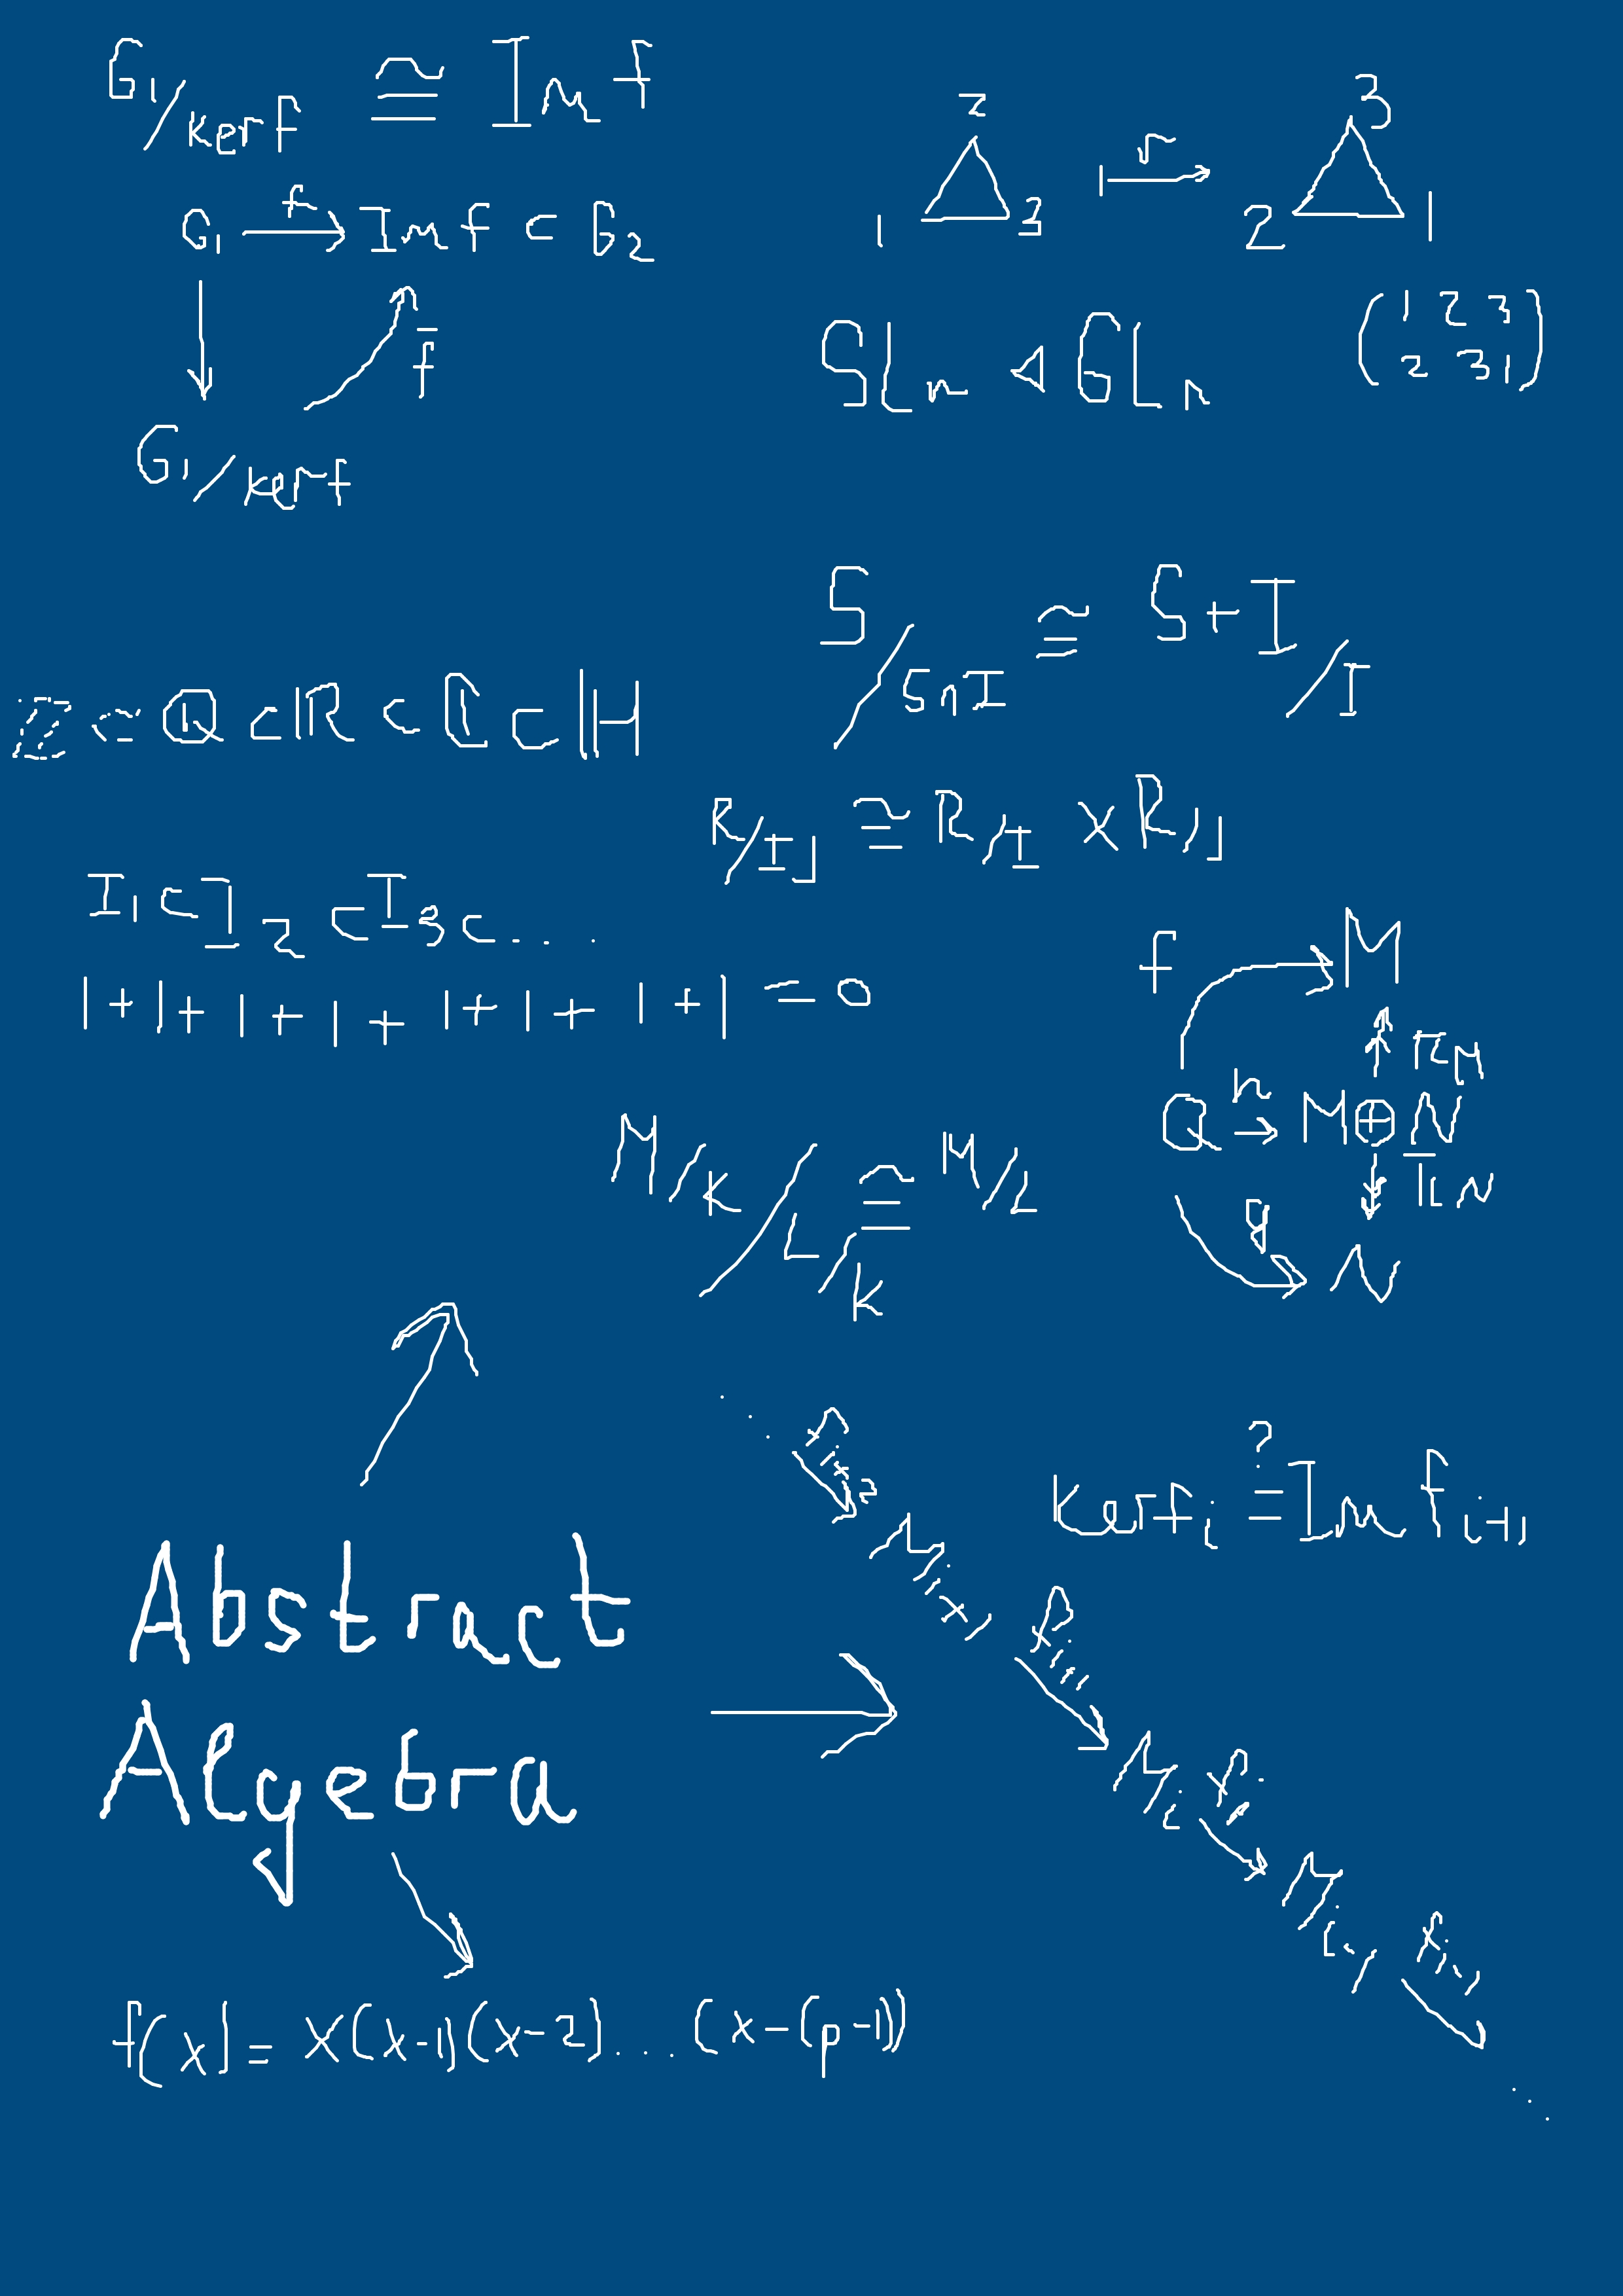
\includepdf[scale=1]{preview.jpg}

\tableofcontents
\newpage

%start Теорія кілець
%\iffalse
\section{Теорія кілець}
\subsection{Означення кільця}
\begin{definition}
Нехай $R$ --- деяка непорожня множина, $+ \colon R \times R \to R$ та $\cdot \colon R \times R \to R$ --- дві бінарні операції.\\
\textbf{Кільцем} назвемо трійку $\left<R, +, \cdot \right>$, для якої виконуються властивості:
\begin{enumerate}[nosep,label={\Roman*.}]
\item Замкненість відносно $+$ (цю операцію називають \textbf{додаванням}):
\begin{align*}
\forall a,b \in R: a+b \in R.
\end{align*}
\item Замкненість відносно $\cdot$ (цю операцію називають \textbf{множенням}):
\begin{align*}
\forall a,b \in R: a \cdot b \in R.
\end{align*}
\item Підпорядкована такими аксіомами:
\begin{align*}
\begin{tabular}{lll}
1) & $\forall a,b,c \in R: a+(b+c) = (a+b)+c$; & (асоціативність додавання) \\
2) & $\forall a,b,c \in R: a+b = b+a$; & (комутативність додавання) \\
3) & $\exists 0 \in R: a+0 = a$; & (існування нейтрального елементу за додаванням) \\
4) & $\forall a \in R: \exists (-a) \in R: a+(-a) = 0$; & (існування оберненого елементу за додаванням) \\
5) & $\forall a,b,c \in R: a \cdot (b \cdot c) = (a \cdot b) \cdot c$; & (асоціативність множення) \\
6) & $\forall a,b,c \in R: \begin{gathered} (a+b)\cdot c = (a\cdot c) + (b \cdot c); \\ c \cdot (a+b) = (c \cdot a) + (c \cdot b). \end{gathered}$ & (дистрибутивність множення відносно додавання) \\
\end{tabular}
\end{align*}
\end{enumerate}
$0 \in R$ називають \textbf{нулем кільця}; $(-a) \in R$ називають \textbf{протилежним елементом} $a \in R$.
\end{definition}

\begin{remark}
Якщо взяти структуру $\left< R, +\right>$, то пункти 1)-4) кажуть, що вона формує абелеву групу. Зокрема звідси вилпиває єдиність $0$ та єдиність протилежного елементу $(-a)$ для кожного $a \in R$.
\end{remark}

\begin{example}
Зокрема $\left<\mathbb{R},+,\cdot\right>$ утворює кільце, де операції $+,\ \cdot$ визначені стандартним чином. 
\end{example}

\begin{example}
Зокрема $\left<\mathbb{R}[x],+,\cdot\right>$ утворює кільце\footnote{До цього кільця ми ще повернемось, оскільки планується певне узагальнення.}, де операції $+,\ \cdot$ визначені таким чином: якщо
\begin{align*}
f(x) = a_0 + a_1x + a_2x^2 + \dots + a_nx^n; \\
g(x) = b_0 + b_1x + b_2x^2 + \dots + b_mx^m,
\end{align*}
то звідси
\begin{align*}
f(x) + g(x) & = (a_0+b_0) + (a_1+b_1)x + \dots + (a_n+b_n)x^n + b_{n+1}x^{n+1} + \dots + b_mx^m; \\
f(x) \cdot g(x) & = a_0b_0 + (a_0b_1+a_1b_0)x + (a_0b_2 + a_1b_1 + a_2b_0)x^2 + \dots \\
& +(a_0b_m+a_1b_{m-1}+\dots+ a_{m-1}b_1 + a_m b_0)x^m.
\end{align*}
(\textit{при множенні вважається, що $a_k = 0$ при $k > n$}).
\end{example}

\begin{example}
Також $\left<\mathbb{Z}_n,+,\cdot\right>$ утворює кільце, де $+,\ \cdot$ визначені так, як коли ми досліджували групи.
\end{example}

\begin{example}
(\textit{для тих, хто трошки теорію міри знає}). Нехай $\mathcal{K}$ --- кільце множин. Перевіримо, що $\left<\mathcal{K},\symdif,\cap\right>$ утворює кільце (\textit{тут $+$ є операція симетричної різниці, а $\cdot$ є взяття перетину}).
\bigskip \\
Те, що $\mathcal{K}$ --- замкнена відносно $\symdif, \cap$, випливає з властивостей кільця з теорії міри. Решта аксіом доводиться аксіоматично зі знань теорії множин, зокрема:
\begin{enumerate}[nosep,wide=0pt,label={\arabic*)}]
\item $A \symdif (B \symdif C) = (A \symdif B) \symdif C$;
\item $A \symdif B = B \symdif A$;
\item $A \symdif \emptyset = A$;
\item $A \symdif A = \emptyset$;
\item $A \cap (B \cap C) = (A \cap B) \cap C$;
\item $A \cap (B \symdif C) = (A \cap B) \symdif (A \cap C)$ та $(B \symdif C) \cap A = (B \cap A) \symdif (C \cap A)$.
\end{enumerate}
Ми маємо, що $\emptyset$ --- нуль кільця, а от протилежним елементом до $A$ буде сама ж $A$.
\end{example}

\begin{proposition}[Властивості]
Нехай $\left<R,+,\cdot \right>$ --- кільце. Тоді:
\begin{enumerate}[nosep, wide=0pt, label={\arabic*)}]
\item $\forall a \in R: 0 \cdot a = a \cdot 0 = 0$;
\item $\forall a,b \in R: a \cdot (-b) = (-a) \cdot b = -(a \cdot b)$;
\item $(-1) \cdot a = -a$.
\end{enumerate}
\end{proposition}

\begin{proof}
\begin{enumerate}[topsep=0pt, wide=0pt, label={\arabic*)}]
\item Спочатку розпишемо ось так:
\[
0 \cdot a = (0 + 0) \cdot a = 0 \cdot a + 0 \cdot a.
\]
Далі за правилом скорочення відносно додавання одержимо $0 \cdot a = 0$.

\item Доведемо, що $a \cdot (-b)$ --- протилежний елемент до $a \cdot b$. Дійсно,
\[
(a \cdot b) + a \cdot (-b) = a \cdot (b + (-b)) = a \cdot 0 = 0.
\]
Отже, $a \cdot (-b) = -(a \cdot b)$.

\item За щойно доведеною властивістю маємо
\[
-a = -(a \cdot 1) = (-1) \cdot a. \qedhere
\]
\end{enumerate}
\end{proof}

\subsection{Підкільця}
\begin{definition}
Нехай $\left<R,+, \cdot \right>$ --- кільце та $R_1 \subset R$ --- деяка підмножина.\\
Підмножина $R_1$ називається \textbf{підкільцем}, якщо 
\begin{align*}
\left<R_1,+,\cdot \right> \text{ --- кільце},
\end{align*}
де додавання та множення ми успадкували з $R$.
\end{definition}

\begin{remark}
Оскільки $\left< R,+\right>$ --- абелева група, то звідси за означенням $\left< R_1,+\right>$ буде підгрупою, а тому в них будуть однакові нульові елементи.
\end{remark}

Для визначення підкільця є ідентичний критерій, що з теорії груп, просто буде додаткова умова.

\begin{theorem}[Критерій підкільця]
\label{subring_criterion}
Нехай $\left<R,+, \cdot \right>$ --- та $R_1 \subset R$ --- підмножина. Тоді
\begin{center}
$R_1$ --- підкільце $\iff \begin{cases} \forall a,b \in R_1: a+b \in R_1; \\ \forall a,b \in R_1: a \cdot b \in R_1; \\ \forall a \in R_1: -a \in R_1; \end{cases}$ та $R_1 \neq \emptyset$.
\end{center}
\textit{Вправа: довести.}
\end{theorem}

\begin{corollary}[Переписаний критерій]
Компактніше можна записати ось так:
\begin{center}
$R_1$ --- підкільце $\iff \begin{cases} \forall a,b \in R_1: a-b \in R_1; \\ a \cdot b \in R_1; \end{cases}$ та $R_1 \neq \emptyset$.
\end{center}
\end{corollary}

\begin{remark}
Під виразом $a-b$ мається на увазі $a + (-1) \cdot b$.
\end{remark}

\begin{example}
Зокрема $\mathbb{Z}, \mathbb{Q}$ --- підкільця кільця $\left< \mathbb{R},+,\cdot \right>$.
\end{example}

\begin{example}
Розглянемо кільце $\left<\mathbb{R}[x], +, \cdot \right>$ та \iffalse Розглянемо множину $\mathbb{R}[0] = \{f(x) \in \mathbb{R}[x]: f(0) = 0\}$ - многочлен без вільного члена. Тоді $\mathbb{R}[0]$ - підкільце - це легко показується.\\ \fi
підмножину $\mathbb{R}_n[x]$ --- многочлени до степені $n$. У цьому випадку $\mathbb{R}_n[x]$ вже не буде підкільцем, тому що хоча $f(x) = g(x) = x^n \in \mathbb{R}_n[x]$, але добуток $f(x) \cdot g(x) = x^{2n} \not \in \mathbb{R}_n[x]$.
\end{example}

\begin{example}
Для кільця $\left<\mathbb{Z},+,\cdot \right>$ множина $n\mathbb{Z} = \{\dots,-2n,-n,0,n,2n,\dots\}$ буде підкільцем.
\end{example}

\begin{remark}
Кожне кільце $\left<R,+,\cdot \right>$ має такі підкільця: $\{0\}$ та $R$.
\end{remark}

\subsection{Основні види кілець}
\subsubsection{Комутативні кільця}
\begin{definition}
Кільце $\left<R,+, \cdot \right>$ називається \textbf{комутативним}\footnote{Про комутативні кільця є багато цікавої додаткової теорії. Зараз я залишати тут не буду, оскільки це лише перші огляди на кільця.}, якщо
\begin{align*}
\forall a,b \in R: a \cdot b = b \cdot a \qquad \text{(комутативність множення)}
\end{align*}
У протилежному випадку --- \textbf{некомутативним}.
\end{definition}

\begin{example}
Зокрема $\left<\mathbb{R},+,\cdot \right>$ --- комутативне кільце.
\end{example}

\begin{example}
А ось $\left< \Mat_{n \times n}(\mathbb{R}), +, \cdot \right>$ --- некомутативне кільце.
\end{example}

\subsubsection{Кільця з одиницею}
\begin{definition}
Кільце $\left<R,+, \cdot \right>$ називається \textbf{кільцем з одиницею}\footnote{Важливе зауваження щодо кільців з одиницями я залишу в окремому немунерованому розділі ''Сучасний підхід до означення кілець''.}, якщо
\begin{align*}
\exists 1 \in R: a \cdot 1 = 1 \cdot a = a
\end{align*}
Тобто існує так званий елемент $1$ --- нейтральний елемент за множенням.
\end{definition}

\begin{proposition}
Якщо $\left<R,+, \cdot \right>$ --- кільце з одиницею, то ця одиниця --- єдина.
\end{proposition}

\begin{proof}
!Припустимо, що існують дві одиниці $1, 1' \in R$, тоді маємо $1 \cdot 1' = 1$, але з іншого боку, $1 \cdot 1' = 1'$, а тому вони рівні. Суперечність!
\end{proof}

\begin{example}
Зокрема $\left<\mathbb{R}[x],+,\cdot \right>$ --- кільце з одиницею $1(x) \equiv 1$.
\end{example}

\begin{example}
Хоча дана структура $\left<\mathcal{K}, \symdif, \cap \right>$ утворює кільце, але без одиниці.
\bigskip \\
Якщо припустити, що деяка множина $I$ --- одиниця кільця, то має виконуватись $A \cap I = I \cap A = A$ для кожної множини $A \in \mathcal{K}$. Але це можливо лише тоді, коли $A \subset I$. У нас в кільці може існувати елемент $A \cup I \in \mathcal{K}$, для якого $A \cup I \supset I$, а також $(A \cup I) \cap I \neq A$. Прийшли до суперечності.
\end{example}

\begin{example}
Але можна показати, що $\left<\mathcal{A}, \symdif, \cap \right>$ --- кільце з одиницею $\iff \mathcal{A}$ --- алгебра множин. \\
Причому одиницею кільця буде універсальна множина $U$.
\end{example}

\begin{lemma}
Нехай $\left<R,+,\cdot \right>$ --- ненульове кільце з одиницею. Тоді $0 \neq 1$ (\textit{отакої, не очікували?}).
\end{lemma}

\begin{proof}
!Припустимо, що все ж таки $0 = 1$. Тоді
\begin{align*}
a \cdot 1 = 1 \cdot a = a; \\
a \cdot 0 = 0 \cdot a = 0.
\end{align*}
Єдина можливість тоді --- це $a = 0$. Але кільце в нас ненульове. Суперечність!
\end{proof}

\begin{remark}
Але кільце $\left< \{0\},+,\cdot \right>$ має одиницю $1 = 0$, тобто збігається з нулем кільця.
\end{remark}

\begin{definition}
Нехай $\left<R,+,\cdot \right>$ --- кільце з одиницею.\\
Елемент $a \in R$ називають \textbf{оборотним} в кільці $R$, якщо
\begin{align*}
\exists a^{-1} \in R: a \cdot a^{-1} = a^{-1} \cdot a = 1.
\end{align*}
Водночас $a^{-1}$ називають \textbf{оберненим} до $a$ в кільці $R$.
\end{definition}

\begin{remark}
Не всі $a \in R$ є оборотними в кільці з одиницею.\\
Зокрема $0 \in R$, але от $a \cdot 0 = 0 \cdot a = 0 \neq 1$ --- і це взагалі для всіх $a \in R$.
\end{remark}

\begin{remark}
Зате у будь-якого ненульового кільця з одиницею $\left<R,+,\cdot \right>$ елементи $1,-1$ будуть завжди оборотними. Дійсно, якщо покласти $1^{-1} = 1$ та $(-1)^{-1} = -1$, то означення оберненості виконується.
\end{remark}

\textit{Позначення}: $R^\times$ --- множина всіх оборотних елементів кільця $\left<R,+,\cdot \right>$.

\begin{example}
Розглянемо кілька прикладів:
\begin{figure}[H]
\centering
\begin{tabular}{c|c}
$R$ & $R^\times$ \\
\hline
$\mathbb{R}$ & $\mathbb{R} \setminus \{0\}$ \\
$\mathbb{Z}$ & $\{-1,1\}$ \\
$\mathbb{Z}_p$ & $\mathbb{Z}_p \setminus \{0\}$ \\
$\mathbb{Z}_n$ & $U_n$ \\
$M_{n \times n}(\mathbb{R})$ & $\mathrm{GL}_n$ \\
\end{tabular}
\end{figure}
Більш детальне пояснення:
\begin{enumerate}[wide=0pt,label={\arabic*)}]
\item Тут всі ненульові елементи оборотні, бо $a \cdot \dfrac{1}{a} = 1$, де елемент $a^{-1} = \dfrac{1}{a}$.
\item Тут лише, $1$, $-1$ оборотні. В інакшому випадку якщо припустити, що для $n \in \mathbb{Z}$ знайдеться обернений $n^{-1} \in \mathbb{Z}$, то маємо $n \cdot n^{-1} = 1 \implies n^{-1} = \dfrac{1}{n}$. Але тоді $n^{-1} \in \mathbb{Z}$ лише в тому випадку, коли $n = \pm 1$.
\item (\textit{див.\ 4)});
\item Обернений елемент $\overline{m} \in \mathbb{Z}_n$ існує $\iff \gcd(m,n) = 1$.
\item Оборотними будуть ті матриці, які мають ненульові визначники.
\end{enumerate}
\end{example}

\begin{example}
Розглянемо так звану множину \textbf{гаусових чисел}
\begin{align*}
\mathbb{Z}[i] = \{ a + bi \mid a,b \in \mathbb{Z},\ i^2 = -1 \}.
\end{align*}
Неважко переконатися, що $\left< \mathbb{Z}[i], +, \cdot \right>$ утворює комутативне кільце. З'ясуємо, чим буде $(\mathbb{Z}[i])^\times$.
\bigskip \\
Нехай $a \in (\mathbb{Z}[i])^\times$, тоді існує $b \in \mathbb{Z}[i]$, для якого $ab = 1$. Позначимо $a = x+iy, b = u+iv$, причому $u,v,x,y \in \mathbb{Z}$. Тоді
\[
(xu-yv) + i(xv+yu) = 1 \iff \begin{cases} xu - yv = 1; \\ xv + yu = 0. \end{cases}
\]
Спочатку випадок $v = 0$ перед тим, як будемо домножувати. Матимемо:
\[
\begin{cases} xu = 1; \\ yu = 0. \end{cases} \iff \begin{cases} x = \pm 1; \\ u = \pm 1; \\ y = 0. \end{cases}
\]
Домножимо перше рівняння на $v \neq 0$, а з другого виразимо $xv = -yu$, отримаємо:
\[
-yu^2 - yv^2 = 1 \iff y(u-v)(u+v) = -1.
\]
Рівняння в цілих числах, а тому ця рівність можлива: або всі $-1$, або один $-1$ і решта два $1$. Будуть чотири випадки, серед яких спрацює один:
\[
\begin{cases} 
y = 1; \\
u - v = -1; \\
u + v = 1;
\end{cases} \implies y = 1, u = 0, v = -1, x = 0.
\]
Таким чином, одержали такі числа: або $a = 1, b = 1$, або $a = -1, b = -1$, або $a = i, b = -i$. Отже,
\begin{align*}
(\mathbb{Z}[i])^\times = \{1,-1,i,-i\}.
\end{align*}
\end{example}

\begin{theorem}
Нехай $\left<R,+,\cdot \right>$ --- кільце з одиницею. Тоді $\left<R^\times, \cdot \right>$ задає групу.
\end{theorem}

\begin{proof}
Маємо $a,b \in R^\times$, тоді вони мають обернені елементи $a^{-1},b^{-1}$. Щоб довести, що $a \cdot b \in R^\times$, треба показати, що існує $(a \cdot b)^{-1}$. І дійсно, якщо покласти $(a \cdot b)^{-1} = b^{-1} a^{-1}$, то маємо
\[
(ab) \cdot (ab)^{-1} = (ab) \cdot (b^{-1}a^{-1}) (a \cdot 1 \cdot a^{-1}) = a \cdot a^{-1} = 1.
\]
Отже, замкненість відносно $\cdot$ вже є.\\
Маємо асоціативність автоматично, за означенням кільця.\\
Нейтральний елемент --- це $1 \in R^\times$, просто тому що $1^{-1} = 1$, а тому $1 \in R^\times$, а також $a \cdot 1 = a$.\\
Маємо $a \in R^\times$. Покажемо, що існує $a^{-1} \in R^\times$, для якого $a \cdot a^{-1} = 1$. Дійсно, для $a \in R^\times$ є обернений $a^{-1} \in R^\times$, водночас для нього є обернений $(a^{-1})^{-1} \overset{\text{покладемо}}{=} a$, а тому $a^{-1} \in R^\times$.
\end{proof}

\begin{example}
Зокрема $\left< \mathbb{R} \setminus \{0\}, \cdot \right>$ --- група. Тепер це можна позначити як $\left< \mathbb{R}^{\times}, \cdot \right>$.
\end{example}

\subsubsection{Області цілісності}
\begin{definition}
Нехай $\left<R,+,\cdot \right>$ --- кільце.\\
Елементи $a \neq 0,b \neq 0$ називають \textbf{дільниками нуля}, якщо
\begin{align*}
ab=0
\end{align*}
Тут $a,b$ --- відповідно лівий та правий дільники нуля.
\end{definition}

\begin{example}
Кільце $\left< \mathbb{Z}_6, +, \cdot \right>$ має три дільників нуля: $\overline{2}, \overline{3}, \overline{4}$. Дійсно,
\[
\overline{2} \cdot \overline{3} = \overline{2} \cdot \overline{4} = \overline{3} \cdot \overline{4} = \overline{0}.
\]
\end{example}

\begin{example}
Кільце $\left< \mathbb{R}, +, \cdot \right>$ не має дільників нуля.
\bigskip \\
Якщо припустити, що такий існує дільник нуля $a \in \mathbb{R}$, то тоді знайдеться елемент $b \in \mathbb{R}$, для якого $ab=0$, але тоді або $a = 0$, або $b = 0$ --- неможливо.
\end{example}

\begin{theorem}
\label{inverses_are_not_zero_divisors}
Нехай $\left<R,+,\cdot \right>$ --- кільце з одиницею. Тоді жодний оборотний елемент не є дільником нуля.
\end{theorem}

\begin{proof}
!Припустимо, що існує такий обернений елемент $a \in R^\times$, який є лівим дільником нуля. Маємо:
\begin{align*}
a \cdot a^{-1} = 1; \\
a \cdot b = 0 \text{ для деякого $b \in R \setminus \{0\}$}.
\end{align*}
Але тоді 
\[
b = b \cdot 1 = b \cdot (a \cdot a^{-1}) = (b \cdot a) \cdot a^{-1} = 0 \cdot a^{-1} = 0.
\]
Одержали суперечність!
\end{proof}

\begin{remark}
Однак якщо елемент --- не дільник нуля, то не обов'язково, що він є оборотним.
\end{remark}

\begin{example}
Зокрема в кільці $\left< \mathbb{Z},+,\cdot \right>$ жодний ненульовий елемент не є дільником нуля, серед них лише $1,-1$ є оборотними.
\end{example}

\begin{theorem}
Нехай $\left<R,+,\cdot \right>$ -- кільце. Тоді справедливе наступне:
\begin{center}
виконуються закони скорочення відносно множення $\iff$ кільце не містить дільників нуля.
\end{center}
\end{theorem}
Під законами скорочення маю на увазі:
\[
\begin{cases}
ax = bx \iff a = b \\
xa = xb \iff a = b
\end{cases}\]
відповідно праве та ліве скорочення, де $x \neq 0$ та $a,b \in R$.

\begin{proof}
\rightproof Дано: можна юзати закон скорочення.\\
!Припустимо, що існує один дільник нуля $a \in R$ (\textit{скажімо, лівий}), тобто $ab = 0$ для $b \neq 0$. Але тоді $a \cdot b = a \cdot 0$, і за правилом (\textit{лівого}) скорочення, $b = 0$. Суперечність!\\
Ми показали таким чином, що якщо можна юзати лише лівий закон скорочення, то тоді кільце не має дільників нуля.
\bigskip \\
\leftproof Дано: нема дільників нуля. Тоді беремо $a,b,x \in R$ так, що $x \neq 0$. Тоді
\[
ax = bx \iff (a-b) \cdot x = 0 \iff a-b = 0 \iff a = b.
\]
Всі еквівалетності виконуються в силу відсутності дільників нуля.  Аналогічно доводиться, що 
\[
xa = xb \iff a = b. \qedhere
\]
\end{proof}

\begin{remark}
Взагалі-то кажучи, у кільці $\left<R, +, \cdot\right>$ не обов'язково вимагати, щоб жодний елемент не був дільником нуля. Достатньо, щоб $x \in R \setminus \{0\}$, на який ми скорочуємо, не був дільником нуля.
\end{remark}

\begin{theorem}
\label{in_finite_ring_non_zero_divisors_are_inverses}
Нехай $\left<R,+,\cdot \right>$ --- скінченне (!) кільце з одиницею та $a \in R$ --- не дільник нуля. Тоді $a$ --- оборотний.
\end{theorem}

\begin{proof}
Розглянемо випадок $\card R = n > 1$, бо коли один, то нема шо доводити.\\
Маємо $a \in R, a \neq 0$ --- не дільник нуля. Шукати обернений елемент будемо за таким же принципом, як це було в \thref{multiplicative_class_of_residues_mod_n_is_a_group}. Розглянемо множину 
\[
a \cdot R = \{a \cdot b \mid b \in R\}.
\]
Покажемо, що тут всі $n$ елементів --- різні. Дійсно,
\[
a \cdot b_1 = a \cdot b_2 \implies a \cdot (b_1-b_2) = 0 \overset{a \text{ не дільник}}{\implies} b_1-b_2 = 0 \implies b_1 = b_2.
\]
Отже, по-перше, $\card R = \card(a \cdot R) = n$, а також по-друге, $a \cdot R \subset R$. Тобто звідси $a \cdot R = R$.\\
Оскільки $1 \in R$, то один з елементів $a \cdot b \in a \cdot R$ має співпадати з $1$. Отже, $\exists b \in R: a \cdot b = 1$ --- довели існування правого оберненого.\\
Аналогічно якщо розглянути $R \cdot a = \{b \cdot a, b \in R \}$, то доведемо існування лівого оберненого.\\
Оскільки $\left<R, \cdot \right>$ утворює моноїд та праві, ліві обернені існують, то вони рівні. Тобто звідси
\[
\forall a \in R: \exists a^{-1} = b \in R: a \cdot a^{-1} = a^{-1} \cdot a = 1. \qedhere
\]
\end{proof}

\begin{example}
Кільце $\left<\mathbb{Z}_p, +, \cdot \right>$, де $p$ --- просте число, не має дільників нуля, тому що
\[
\overline{k_1} \cdot \overline{k_2} = \overline{k_1 \cdot k_2} = \overline{0} \implies k_1 \cdot k_2 \equiv 0 \pmod p \implies p \mid k_1 \cdot k_2,
\]
тобто або $p \mid k_1 \implies \overline{k_1} = \overline{0}$; або $p \mid k_2 \implies \overline{k_2} = \overline{0}$. Тоді звідси випливає, що всі ці елементи --- оборотні, тобто $\mathbb{Z}_p^\times = \mathbb{Z}_p \setminus \{0\}$.\\
\textit{Це як по-іншому можна було довести існування обернених елементів.}
\end{example}

\begin{definition}
Комутативне кільце $\left<R,+,\cdot \right>$ з одиницею називається \textbf{областю цілісності} (англ. \textbf{integral domain}), якщо
\begin{align*}
R \text{ не містить дільників нуля.}
\end{align*}
\end{definition}

\begin{example}
Зокрема кільця $\mathbb{Z},\ \mathbb{Z}_p$ (\textit{тут $p$ --- просте число}) будуть областями цілісності.
\end{example}

\begin{example}
Але кільце $\mathbb{Z}_6$ уже не буде областю цілісності, бо там є дільники нуля за прикладом вище.
\end{example}

\iffalse
\begin{remark}
Ще раз наголошу собі. Елемент $a$ - дільник нуля, якщо $0 = ab$, де $a,b$ взагалі ненулеві. Інакше це можна позначати як $a \mid 0$. І таким чином, грубо кажучи, $0$ ділиться націло на ненульовий елемент - а результат залишається ненульовим, що дивно для природного розуміння.\\
Тому зазвичай розглядають область цілісності, де такого не відбувається.
\end{remark}
\fi

\subsubsection{Поле}
\begin{definition}
Ненульове комутативне кільце $\left<F,+,\cdot \right>$ з одиницею називається \textbf{полем}, якщо
\begin{align*}
F^\times = F \setminus \{0\},
\end{align*}
тобто всі ненульові елементи --- оборотні.
\end{definition}

\begin{example}
Зокрема $\left<\mathbb{Q},+,\cdot \right>$ буде полем.
\end{example}

\begin{example}
Розглянемо ще ось таку множину
\begin{align*}
\mathbb{Q}(\sqrt{2}) = \{a + b \sqrt{2} \mid a,b \in \mathbb{Q}\}.
\end{align*}
Тоді структура $\left< \mathbb{Q}(\sqrt{2}), +, \cdot \right>$ задаватиме також поле.
\end{example}

\begin{corollary}
Будь-яке поле --- область цілісності.\\
\textit{Випливає з} \thref{inverses_are_not_zero_divisors}.
\end{corollary}

\begin{remark}
Але не кожна область цілісності --- поле (\textit{наприклад, кільце $\mathbb{Z}$}).
\end{remark}

\begin{theorem}
Якщо $R$ --- скінченна область цілісності, яка містить не менше $2$ елементів, то $R$ --- поле.\\
\textit{Випливає з} \thref{in_finite_ring_non_zero_divisors_are_inverses}.
\end{theorem}

\begin{example}
Зокрема $\mathbb{Z}_p$ (\textit{тут $p$ --- просте число}) буде полем.
\bigskip \\
А ось якщо $p$ --- складене, то тоді вже полем не буде, тому що має дільник нуля. Дісно, маємо $p = k \cdot m$, оскільки $p$ уже складене. Тоді 
\[
\overline{0} = \overline{p} = \overline{k \cdot m} = \overline{k} \cdot \overline{m}.
\]
\end{example}
\noindent
Про поле будемо говорити детальніше пізніше.


\subsection{Характеристика}
\begin{definition}
Нехай $\left< R, +, \cdot \right>$ --- ненульове кільце.\\
\textbf{Характеристикою} кільця називають найменше число $n \in \mathbb{N}$, для якого
\begin{align*}
\forall r \in R: \underbrace{r+\dots+r}_{n\text{ разів}} = 0.
\end{align*}
Позначення: $n = \charac(R)$.\\
Якщо такого $n \in \mathbb{N}$ не існує, то тоді $\charac(R) \eqbydef 0$.
\end{definition}

\begin{remark}
Інколи ще скорочують $\underbrace{r+\dots+r}_{n\text{ разів}} = n \cdot r$.
\end{remark}

\begin{example}
Зокрема в кільці $\left< \mathbb{R},+,\cdot \right>$ маємо $\charac(\mathbb{R}) = 0$ (\textit{тут все зрозуміло}).
\end{example}

\begin{proposition}
Нехай $\left<R, +, \cdot \right>$ --- кільце з одиницею. Відомо, що $\ord_{\left<R,+ \right>}(1) = n$. Тоді $\charac R = n$.
\end{proposition}

\begin{proof}
Позначимо $\charac = m$. Тоді маємо 
\[
\underbrace{1 + \dots + 1}_{m \text{ разів}} = 0 \implies \ord(1) = n \mid m \implies n \leq m.
\]
Водночас 
\[
\underbrace{r + \dots + r}_{n \text{ разів}} = r(\underbrace{1 + \dots + 1}_{n \text{ разів}}) = r \cdot 0 = 0 \implies m \geq n.
\]
Отже, $m = n$.
\end{proof}

\begin{remark}
Отже, коли ми маємо ненульове кільце з одиницею $\left< R,+,\cdot\right>$, то характеристикою назвають найменше число $n \in \mathbb{N}$, для якого
\begin{align*}
\underbrace{1+ \dots + 1}_{n \text{ разів}} = 0.
\end{align*}
або характеристика дорівнює $0$, якщо такого найменшого нема. І саме ось таке означення дають більшість авторів.
\end{remark}

\begin{example}
Зокрема в кільці $\left< \mathbb{Z}_n, +, \cdot \right>$ маємо $\text{char}(\mathbb{Z}_n) = n$.
\end{example}

\begin{proposition}
Нехай $\left<R, +, \cdot \right>$ --- область цілісності. Тоді $\charac (R) \in \{0,p\}$, де $p$ --- просте число.
\end{proposition}

\begin{proof}
Якщо $\charac R = 0$, то нема що доводити. Тому нехай $\charac R = n$.\\
!Припустимо, що $n$ --- складене число, тоді $n = ab$, причому $1 < a,b < n$. Звідси
\[
0 = \underbrace{1 + \dots + 1}_{n \text{ разів}} = \underbrace{\underbrace{1 + \dots + 1}_{a \text{ разів}} + \dots + \underbrace{1 + \dots + 1}_{a \text{ разів}}}_{b \text{ разів}} = (\underbrace{1 + \dots + 1}_{a \text{ разів}})(\underbrace{1 + \dots + 1}_{b \text{ разів}}).
\]
В останній рівності ми скористались дитрибутивністю, коли виносили $\underbrace{1 + \dots + 1}_{a \text{ разів}}$. Тепер, оскільки ми знаходимось в області цілісноті, то тоді або $\underbrace{1 + \dots + 1}_{a \text{ разів}} = 0$, або $\underbrace{1 + \dots + 1}_{b \text{ разів}} = 0$. Звідси отримаємо або $a \geq n$, або $b \geq n$. У двох випадках суперечність!\\
Отже, $n$ може бути лише простим числом.
\end{proof}

\subsection{Кільце многочленів}
(TODO: ще формувати)
\bigskip \\
Задано $\left< R,+,\cdot \right>$ -- будь-яке кільце. Визначимо таку множину:
\begin{align*}
R[x] = \{a_0 + a_1 x + \dots + a_n x^n \mid n \geq 0, a_i \in R\},
\end{align*}
де елемент $f \in R[x]$ -- многочлен, $f(x) = a_0 + a_1 x + \dots + a_n x^n$. Даний об'єкт можна ще записати таким чином: $f(x) = \displaystyle\sum_{i \geq 0} a_i x^i$, де у випадку $i > n$ матимемо $a_i = 0$.\\
Нехай $f(x) = \displaystyle\sum_{i \geq 0} a_i x^i,\ g(x) =\sum_{i \geq 0} b_i x^i$. Ми визначимо такі операції:
\begin{align*}
f(x) + g(x) = \displaystyle\sum_{i \geq 0} (a_i + b_i) x^i \\
f(x) \cdot g(x) = \displaystyle\sum_{i \geq 0} \left(\sum_{r + s = i} a_r \cdot b_s \right) x^i
\end{align*}
Це такі самі операції, як з многочлени з дійсними коефіцієнтами. Зрозуміло, що множина -- замкнена відносно цих операцій.

\begin{theorem}
$\left<R[x],+,\cdot\right>$ -- (комутативне з одиницею) кільце $\iff \left< R,+,\cdot \right>$ -- (комутативне з одиницею) кільце.
\end{theorem}

\begin{proof}
Буде раціональніше спочатку довести в зворотному напрямку.\\
\leftproof Дано $\left< R,+,\cdot\right>$ -- кільце. Наша мета: $\left<R[x],+,\cdot\right>$ -- кільце.\\
Візьмемо многочлени $f,g,h \in R[x]$, тобто $f(x) = \displaystyle\sum_{i \geq 0} a_i x^i \quad g(x) = \displaystyle\sum_{i \geq 0} b_i x^i \quad h(x) = \displaystyle\sum_{i \geq 0} c_i x^i$.\\
1. $f(x) + (g(x) + h(x)) = f(x) + \displaystyle\sum_{i \geq 0} (b_i + c_i) x^i = \sum_{i \geq 0} (a_i + (b_i + c_i)) x^i \overset{1) \text{ для } R}{=} \sum_{i \geq 0} ((a_i + b_i) + c_i) x^i = (f(x)+g(x)) + \sum_{i \geq 0} c_i x^i = (f(x)+g(x)) + h(x)$.\\
2. $f(x) + g(x) = \displaystyle\sum_{i \geq 0} (a_i + b_i) x^i \overset{2) \text{ для } R}{=} \sum_{i \geq 0} (b_i + a_i) x^i = g(x) + f(x)$.\\
3. Маємо $\textbf{0}(x) = 0$, тобто $\textbf{0}(x) = \displaystyle\sum_{i \geq 0} 0x^i$, де $0$ - це нуль кільця $R$. Тоді \\ $f(x) + \textbf{0}(x) = \displaystyle\sum_{i \geq 0} (a_i + 0) x^i \overset{3) \text{ для } R}{=} \sum_{i \geq 0} a_i x^i = f(x)$.\\
4. Для $f \in R[x]$ існує $-f \in R[x]$, що $(-f)(x) = \displaystyle\sum_{i \geq 0} (-a_i) x^i \in R[x]$. Оскільки $a_i \in R, i \geq 0$, то за 4), існують $-a_i \in R$ для яких виконується рівність 4). Тоді \\
$f(x) + (-f)(x) = \displaystyle\sum_{i \geq 0} (a_i + (-a_i)) x^i \overset{4) \text{ для } R}{=}  \sum_{i \geq 0} 0 x^i = \textbf{0}(x)$.
\bigskip \\
5. $f(x) \cdot (g(x) \cdot h(x)) \overset{?}{=} (f(x) \cdot g(x)) \cdot h(x)$ -- доволі складна рівність.\\
$g(x) \cdot h(x) = \displaystyle\sum_{i \geq 0} d_i x^i$, де \quad $d_i = \displaystyle\sum_{r + s = i} b_r c_s$\\
$f(x) \cdot (g(x) \cdot h(x)) = \displaystyle\sum_{i \geq 0} u_i x^i$, де \\
$u_i = \displaystyle\sum_{r+s=i} a_r d_s = \sum_{r+s=i} a_r \left( \sum_{\xi + \eta = s} b_\xi c_\eta \right) = \sum_{r+s=i} \sum_{\xi + \eta = s} a_r b_\xi c_\eta = \sum_{\xi+\eta+r=i} a_r b_\xi c_\eta$.\\
\bigskip \\
$f(x) \cdot g(x) = \displaystyle\sum_{i \geq 0} \tilde{d_i} x^i$, де \quad $\tilde{d_i} = \displaystyle\sum_{r+s=i} a_r b_s$\\
$(f(x) \cdot g(x)) \cdot h(x) = \displaystyle\sum_{i \geq 0}v_i x^i$, де \\
$v_i = \displaystyle\sum_{r+s=i} d_r c_s = \sum_{r+s=i} \left( \sum_{\xi + \eta = r} a_\xi b_\eta \right) c_s = \sum_{r+s=i} \sum_{\xi + \eta = r} a_\xi b_\eta c_s = \sum_{\eta + s + \xi = i} a_\xi b_\eta c_s$.\\
Якщо уважно придивитися, то можна зауважити, що $u_v = v_i$, тоді\\
$f(x) \cdot (g(x) \cdot h(x)) = \displaystyle\sum_{i \geq 0} u_i x^i = \sum_{i \geq 0} v_i x^i = (f(x) \cdot g(x)) \cdot h(x)$.\\
Слід також зауважити, що ми користувалися спочатку $6)$ для $R$, а в кінці $5)$ для $R$, просто останнє я це явно не вказав.
\bigskip \\
6. $f(x) \cdot (g(x)+h(x)) = \displaystyle\sum_{i \geq 0} \left( \sum_{r+s=i} a_r (b_s + c_s) \right) x^i = \sum_{i \geq 0} \left( \sum_{r+s=i} a_r b_s + \sum_{r+s=i} a_r c_s \right) x^i = \\ =\sum_{i \geq 0} \left( \sum_{r+s=i} a_r b_s \right) x^i + \sum_{i \geq 0} \left( \sum_{r+s=i} a_r c_s \right) x^i = f \cdot g(x) + f(x) \cdot h(x)$.\\
Аналогічно $(f(x)+g(x)) \cdot h(x) = f(x) \cdot h(x) + g(x) \cdot h(x)$.
\bigskip \\
Тепер нехай $\left< R,+,\cdot\right>$ додатково комутативне кільце з одиницею. Тоді для $f,g \in R[x]$ маємо:\\
$f(x) \cdot g(x) = \displaystyle\sum_{i \geq 0} \left( \sum_{r+s=i} a_r b_s \right)x^i = \sum_{i \geq 0} \left( \sum_{s+r=i} b_s a_r \right)x^i = g \cdot f$.\\
Маємо $\textbf{1}(x) = 1$, тобто $\textbf{1}(x) = 1 + \displaystyle\sum_{i \geq 1} 0x^n$, де $1$ - це одиниця кільця $R$.\\
$f(x) \cdot \textbf{1}(x) = \displaystyle\sum_{i \geq 0} \left( \sum_{\substack{r+s=i \\ s > 0}} a_r \cdot 0 + \sum_{\substack{r+s=i \\ s=0}} a_r \cdot 1 \right) x^i = \sum_{i \geq 0} a_i x^i = f(x)$.\\
Висновок: $\left< R[x],+,\cdot\right>$ -- (комутативне з одиницею) кільце.
\bigskip \\
\rightproof Дано: $\left< R[x],+,\cdot\right>$ -- (комутативне з одиницею) кільце. Варто зауважити, що коли $u \in R$, то автоматично $u \in R[x]$. Тому що $u = u + 0x + 0x^2 + \dots$ Ну тобто, по суті кажучи, ми маємо $R \subset R[x]$. Треба лише довести, що $R$ є підкільцем $R[x]$, але це неважко.
\end{proof}

\begin{corollary}
$\left< R[x],+,\cdot\right>$ -- область цілісності $\iff \left< R,+,\cdot\right>$ -- область цілісності.
\end{corollary}

\begin{proof}
\leftproof Дано: $\left< R,+,\cdot\right>$ -- область цілісності. По суті, все, що нам залишилось довести, -- це відсутність дільників нуля в $R[x]$.\\
!Припустимо, що $f \in R[x], f \neq \textbf{0}$ -- дільник нуля, тобто $\exists g \in R[x], g \neq \textbf{0}$, для якого $f \cdot g = \textbf{0}$. Тобто маємо $(a_0+a_1 x + \dots + a_nx^n)(b_0 + b_1x + \dots + b_k x^k) = 0$. Маємо старший коефіцієнт $a_n b_k$ після множення. Оскільки многочлен нульовий, то це означає, що всі коефіцієнти, зокрема $a_n b_k = 0$. Але нам відомо, що $a_n,b_k \neq 0$, а тому $a_n$ -- дільник нуля -- суперечить умові того, що $R$ -- область цілісності!
\bigskip \\
\rightproof Дано: $\left< R[x], +, \cdot \right>$ -- область цілісності.\\
!Припустимо, що $u \in R, u \neq 0$ -- дільник нуля, тобто $\exists v \in R, v \neq 0$, для якого $uv = 0$. Але $u$,$v$ можна сприймати як многочлени, і тоді $u$ - дільник нуля в $R[x]$ - суперечність!
\end{proof}

\begin{remark}
Якщо $R$ -- кільце, тобто $R[x]$ -- теж кільце (некомутативне), то нам варто вважати, що $x$ комутує з усіма елементами $a \in R$. Це робиться, аби можна було розкривати дужки.
\end{remark}

\begin{example}
Зокрема маємо $\mathbb{Z}/_{2 \mathbb{Z}}[x]$ -- кільце. Маємо многочлен $f(x) = x(x+\bar{1}) = x^2 + \bar{1}x = x^2 + x$.\\
Можна зауважити, що $\forall x \in \mathbb{Z}/_{2 \mathbb{Z}}: f(x) = \bar{0}$. Але в жодному разі $f(x) \ne \textbf{0}(x)$ як многочлени. У функціональному сенсі вони рівні, але об'єкти різні.
\end{example}

\begin{remark}
Маємо $\left<R,+,\cdot,\right>$ -- кільце, ну тоді вже ясно, що $\left<R[x],+,\cdot,\right>$ -- кільце. Але можна піти далі та утворити нове кільце $\left<R[x][y],+,\cdot,\right>$. Подивимось, що з себе представляє об'єкт $f \in R[x][y]$.\\
$(f(x))(y) = \displaystyle\sum_{j \geq 0} a_j y^j$, при цьому $a_j \in R[x]$, тобто $a_j(x) = \displaystyle\sum_{i \geq 0} b_{ij} x^i$.\\
$(f(x))(y) = \displaystyle\sum_{j \geq 0} \left(\sum_{i \geq 0} b_{ij} x^j\right) y^i$.\\
Далі $(f(x))(y)$ можна позначити за $f(x,y)$, а тому звідси отримаємо \textbf{многочлен з двома змінними}:\\
$f(x,y) = \displaystyle\sum_{i,j \geq 0} b_{ij} x^i y^j$.\\
Надалі можна $R[x][y]$ позначити як $R[x,y]$.
\bigskip \\
Можна далі продовжити цей процес та утворити кільце $R[x_1,x_2,\dots,x_n]$.
\end{remark}

Про кільце многочленів ми ще будемо розмовляти неодноразово.

\subsection{Ідеал кільця. Породжені ідеали}
\begin{definition}
Нехай $\left<R,+,\cdot \right>$ --- кільце.\\
\textbf{Ідеалом} даного кільця назвемо множину $\emptyset \neq J \subset R$, для якої
\begin{align*}
\left<J,+ \right> \text{--- підгрупа групи } \left<R,+\right>; \\
\forall r \in R: \forall j \in J: rj, jr \in J.
\end{align*}
\end{definition}

\begin{remark}
Можна сказати, що ідеал кільця --- це такий собі аналог нормальної підгрупи в теорії груп.
\end{remark}

\begin{remark}
Інколи розрізняють: ліві ідеали, коли $rj \in J$, та праві ідеали, коли $jr \in J$. Якщо ідеал одночасно лівий та правий, інколи це називають двостороннім ідеалом.
\end{remark}

\begin{example}
Розглянемо кільце $\left< \mathbb{Z},+,\cdot \right>$. Воно має ідеали $n \mathbb{Z}$, де $n \in \mathbb{N} \cup \{0\}$, тому що:\\
$n\mathbb{Z}$ --- підгрупа групи $\left<\mathbb{Z},+ \right>$;\\
$\forall m \in \mathbb{Z}: \forall k \in n\mathbb{Z}$ маємо $k = nl$, а тому звідси $mk = km = n(lm) \in n\mathbb{Z}$.
\end{example}

\begin{example}
$\{0\}, R$ --- ідеали кільця $\left<R,+,\cdot \right>$, вони ще називаються \textbf{тривіальними ідеалами}.
\end{example}

\begin{remark}
Якщо $J$ -=- ідеал, то $J$ буде підкільцем $R$. Навпаки --- ні.
\bigskip \\
Зокрема $\mathbb{Z}$ буде підкільцем $\left<\mathbb{R},+,\cdot\right>$, але не ідеалом, тому що $3 \cdot \sqrt{2} \not \in \mathbb{Z}$.
\end{remark}

\begin{proposition}
Нехай $\left<R,+,\cdot \right>$ --- кільце з одиницею та $J$ --- ідеал, для якого $1 \in J$. Тоді $J = R$.
\end{proposition}

\begin{proof}
Те, що $J \subset R$, --- це за означенням.\\
Оскільки $J-$ -- ідеал, то тоді для числа $1 \in J$ та для будь-якого $x \in R$ маємо, що $x \cdot 1 = x \in J$. Тобто $R \subset J$.
\end{proof}

\begin{lemma}
Нехай $\left<R,+,\cdot \right>$ --- комутативне кільце з одиницею, $a \in R$. Тоді $aR$ --- ідеал для цього кільця. Його ще називають \textbf{головним ідеалом, породженим елементом} $a \in R$.\\
\textit{Позначення}: $aR = (a)$.
\end{lemma}

\begin{proof}
Дійсно, маємо
\[
x_1,x_2 \in aR \implies \begin{cases} x_1 = ar_1 \\ x_2 = ar_2 \end{cases}, \text{ де } r_1,r_2 \in R \implies x_1-x_2 = a(r_1-r_2) \implies x_1-x_2 \in aR.
\]
Цим показали, що $aR$ --- підгрупа групи $\left<R,+ \right>$. Крім того,
\[
x \in aR,r_0 \in R \implies x = ar, r \in R \implies r_0 x = xr_0 = arr_0 \in aR.
\]
А цим показали другу умову для ідеала.
\end{proof}

\begin{proposition}
Нехай $\left<R,+,\cdot \right>$ --- комутативне кільце з одиницею, $a \in R$. Тоді $(a)$ --- найменший ідеал, що містить елемент $a$.
\end{proposition}

\begin{proof}
Припустимо, що існує якийсь інший ідеал $J \ni a$, який менший, тобто $J \subset (a)$. Доведемо, що $J = (a)$.\\
Нехай $x \in (a)$, тобто $x = ar_0, r_0 \in R$. Оскільки $J$ --- ідеал, то звідси $\forall j \in J: \forall r \in R: jr \in J$.\\
Зокрема для $j = a$, $r = r_0$ ми маємо $ar_0 = x \in J$. Отже, $(a) \subset J$, а тому звідси $J = (a)$.
\end{proof}

\begin{remark}
Ми знаємо, що $(a) = \{ ar \mid r \in \mathbb{R} \}$. Ми можемо узагальнити означення та написати ідеал, породжений кількома елементами:
\begin{align*}
(a_1,\dots,a_n) = \{r_1 a_1 + \dots + r_n a_n \mid r_1,\dots,r_n \in R\}.
\end{align*}
Те, що це дійсно ідеал, неважко переконатися. Причому найменший, що містить $a_1,\dots,a_n$.
\end{remark}

\begin{example}
Розглянемо кільце $\left< \mathbb{Z},+,\cdot \right>$. Тоді $(n) = (-n) = n \mathbb{Z}$.
\end{example}

\begin{example}
Розглянемо кільце $\left<\mathbb{R}[x],+,\cdot \right>$. Тоді
\[
(p(x)) = \{s \in \mathbb{R}[x]: s(x) = p(x)q(x), q \in \mathbb{R}[x] \},
\]
тобто головний ідеал $(p(x))$ містить многочлени, що діляться націло на многочлен $p$. Випливає з прямого визначення головного ідеала.
\[
(x-a) = \{s \in \mathbb{R}[x]: s(x) = (x-a)q(x), q \in \mathbb{R}[x]\}.
\]
тобто головний ідеал $(x-a)$ містить многочлени, що мають корень $a$.
\end{example}

\begin{remark}
$\{0\}$. $R$ --- головні ідеали комутативного кільця $\left<R,+,\cdot\right>$ з одиницею, тому що
\[
\{0\} = 0R = (0), \qquad R = 1R = (1).
\]
\end{remark}

\begin{definition}
\textbf{Областю} (або \textbf{кільцем}) \textbf{головних ідеалів} називаємо область цілісности, що містить лише головні ідеали.\\
Англійською це називається \textbf{principle ideal domain (PID)}.
\end{definition}

\begin{example}
Зокрема $\left<\mathbb{Z},+,\cdot \right>$ --- що є областю цілісності --- буде областю головних ідеалів.
\bigskip \\
!Припустимо, що $J$ -- деякий ненульовий ідеал, але не можна розписати його як головний ідеал. Щоб прийти до суперечності, ми покажемо, що $J = (m)$ для числа $m = \displaystyle \min_{\substack{n \in \mathbb{N} \\ n \in J}} n$.\\
Цей мінімум завжди існує, тому що коли є якесь від'ємне число $-m \in J$, то зокрема $m = (-1) \cdot (-m) \in J$ в силу означення ідеала.\\
Маємо $m \in J$ та $k \in \mathbb{Z}$, тоді звідси $mk \in J$, а тому $(m) \subset J$.\\
Маємо $n,m \in J$, застосуємо алгоритм Евкліда --- отримаємо
\[
n = km + r \implies r = n - km \in J.
\]
Також $0 \leq r < m$. А оскільки $m$ --- найменше додатне число, то в силу того, що $r \in J$ маємо $r \geq m$. Тому єдиний варіант --- це вимагати $r = 0$.\\
Отже, $n \in J$, причому $n = km$, звідси $n \in (m)$. Отже, $J \subset (m)$.\\
Таким чином, $J = (m)$. Суперечність!
\end{example}

\begin{example}
Зокрема $\left<\mathbb{R}[x],+,\cdot \right>$ --- що є областю цілісності --- буде областю головних ідеалів. Ідея доведення аналогічна. Насправді ці два приклади можна буде узагальнити (\textit{це буде пізніше}).
\iffalse
!Припустимо, що $J$ - деякий ненульовий ідеал, але не можна розписати його як головний ідеал. Щоб прийти до суперечності, ми покажемо, що $J = (p(x))$, де $p$ - многочлен, для якого $\deg p = m$, а число $m = \displaystyle\min_{f \in J} \deg f$, де $m > 0$.\\
Маємо $p(x) \in J$ - многочлен степені $m$. Тоді $\forall q(x) \in \mathbb{R}[x]$ маємо $r(x) = p(x) q(x) \in J$ за означенням ідеала. Отже, $r(x) \in (p(x))$.\\
Таким чином, $(p(x)) \subset J$.\\
Маємо $s(x), p(x) \in J$, застосуємо алгоритм Евкліда - отримаємо\\
$s(x) = p(x)q(x) + r(x) \implies r(x) = s(x) - p(x)q(x) \in J$.\\
Також $\deg r < m$ або $r \equiv 0$. А оскільки $m$ - найменше додатне число, то в силу того, що $r(x) \in J$ ми маємо $\deg r \geq m$. Єдиинй варіант - це $r = 0$, тоді звідси $s(x) = p(x)q(x) \implies s(x) \in (p(x))$. І звідси $J = (p(x))$. Суперечність!
\bigskip \\
І взагалі, якщо ми маємо $k[x]$, де $k$ - деяке поле (див. нижче), то ми все одно будемо мати область головних ідеалів.
\fi
\end{example}

\begin{example}
А от $\left<\mathbb{R}[x_1,\dots,x_n], +, \cdot \right>$ уже не буде областю головних ідеалів.\\
\textit{Поки без доведення}.
\end{example}

\begin{theorem}
Нехай $\left< F,+,\cdot\right>$ --- ненульове комутативне кільце з $1$. Тоді
\begin{center}
$\left<F,+,\cdot\right>$ --- поле $\iff F$ містить лише тривіальні ідеали.
\end{center}
\end{theorem}

\begin{proof}
\rightproof Дано: $\left<F,+,\cdot,\right>$.\\
!Припустимо, що існує якийсь інший ідеал $J \neq \{0\}$ та $J \neq F$. Тоді
\[
\forall j \in J: \forall f \in F: jf \in J.
\]
Зокрема якщо $j \in J$ такий, що $j \neq 0$, то по-перше, $j \in F$, а по-друге, $\exists j^{-1} \in F$. Звідси випливає, що $j \cdot j^{-1} = 1 \in J$. За попереднім твердженням, $J = F$. Суперечність!
\bigskip \\
\leftproof Дано: існують лише тривіальні ідеали.\\
Нехай $a \in F$, де $a \neq 0$, розглянемо головний ідеал $(a)$. Тоді звідси $(a) = R$. Зокрема оскільки $1 \in R$, то звідси $\exists \tilde{a} \in (a) = R: a \tilde{a} = 1$. Отже, всі ненульові елементи --- оборотні, а тому $F$ --- поле.
\end{proof}

\begin{example}
Зокрема поле $\left< \mathbb{R},+,\cdot \right>$ має лише ідеали $\{0\}$ та $\mathbb{R}$.
\end{example}

\subsection{Сума, перетин та добуток ідеалів}
\begin{definition}
Нехай $\left<R,+,\cdot\right>$ --- кільце та $I,J$ --- ідеали $R$.\\
\textbf{Перетином ідеалів $I,J$} називають ідеал $I \cap J$.\\
\textbf{Сумою ідеалів $I,J$} називають ідеал
\begin{align*}
I+J \eqbydef \{ a+b \mid a \in I, b \in J \}.
\end{align*}
\textbf{Добутком ідеалів $I,J$} називають ідеал
\begin{align*}
IJ \eqbydef \{ a_1 b_1 + \dots + a_n b_n \mid a_i \in I, b_i \in J\}
\end{align*}
\end{definition}

\begin{proposition}
$I \cap J,\ I + J,\ IJ$ є дійсно ідеалами кільця $R$.
\end{proposition}

\begin{proof}
I. \textit{$I \cap J$ --- ідеал}.\\
Спочатку доводимо, що $I \cap J$ --- підгрупа $\left< R, + \right>$. Нехай $u,v \in I \cap J$. Розглянемо елемент $u-v$.\\
За умовою, $I$ --- підгрупа $\left<R,+\right>$, тому $u-v \in I$;\\
За умовою, $J$ --- підгрупа $\left<R,+\right>$, тому $u-v \in J$.\\
Разом отримали $u-v \in I \cap J$.\\
Нехай $u \in I \cap J$ та $r \in R$. Тоді оскільки $u \in I$, то тоді $ru, ur \in I$; оскільки $u \in J$, то тоді $ru, ur \in J$. Отримали, що $ru, ur \in I \cap J$.
\bigskip \\
II. \textit{$I+J$ --- ідеал}.\\
Спочатку доводимо, що $I + J$ --- підгрупа $\left< R, + \right>$. Нехай $u,v \in I + J$, тобто $u = a_1 + b_1$ та $v = a_2 + b_2$, елементи $a_1,a_2 \in I,\ b_1,b_2 \in J$. Тоді $u - v = (a_1 - a_2) + (b_1 - b_2)$, причому оскільки $I,J$ --- підгрупи $\left< R,+ \right>$, то тоді $a_1 - a_2 \in I,\ b_1 - b_2 \in J$. Отже, $u-v \in I+J$.\\
Нехай $u \in I+J$, тобто $u = a+b$ при $a \in I,b \in J$, та нехай $r \in R$. Тоді звідси $ur = ar + br$, причому звідси $ar \in I, br \in J$ в силу властивості ідеалу. Отже, $ur \in I+J$. Аналогічним чином доводиться $ru \in I+J$.
\bigskip \\
III. \textit{$IJ$ --- ідеал}.\\
Нехай $u,v \in IJ$, тобто
\begin{align*}
u = a_1^1 b_1^1 + \dots + a_n^1 b_n^1;
v = a_1^2 b_1^2 + \dots + a_m^2 b_m^2.
\end{align*}
Кожний $a_i^j \in I,\ b_i^j \in J$. Тоді маємо
\[
u - v = a_1^1 b_1^1 + \dots + a_n^1 b_n^1 - a_1^2 b_1^2 - \dots - a_m^2 b_m^2.
\]
Ясно, що звідси $u - v \in IJ$.\\
Нехай $u \in IJ$, тобто $u = a_1b_1 + \dots + a_nb_n$ при $a_i \in I, b_i \in J$, та нехай $r \in R$. Тоді звідси
\[
ur = a_1 b_1 r + \dots + a_n b_n r.
\]
Зауважимо, що в цьому випадку $b_i r \in J$ і досі $a_i \in I$ тоді звідси $ur \in IJ$. Тепер з іншого боку, 
\[
ru = r a_1 b_1 + \dots + r a_n b_n.
\]
А тут вже $r a_i \in I$ і досі $b_i \in J$, тоді звідси $ru \in IJ$.
\end{proof}

\begin{remark}
Ми визначили $IJ$ тіпа як скалярний добуток елементів з $I$ та з $J$. Виникає питання, чому ми не позначили $IJ = \{ab \mid a \in I, b \in J\}$. Тому що якщо розписати доведення, то виникнуть проблеми з формуванням підгрупи групи $\left<R,+\right>$.
\end{remark}

\begin{example}
Розглянемо кільце $\mathbb{Z}[x]$ та ідеали $I = (2,x),\ J = (3,x)$. Зауважимо, що $IJ = (6,x)$. Справді, $6 = 2 \cdot 3$, де $2 \in I, 3 \in J$, тож звідси $6 \in IJ$. Також $x = 3x - 2x$, де $3x \in J,\ 2x \in I$, тож звідси $x \in IJ$. Отже, $(6,x) \subset IJ$. Те, що $IJ \subset (6,x)$, довести неважко.\\
При цьому $IJ \neq \{ ab \mid a \in I, b \in J \}$. Тому що $x \in IJ$, а елемент $x$ не розписується як добуток елементів з $I$ та $J$.
\end{example}

\begin{example}
Розглянемо кільце $\mathbb{Z}$ та головні ідеали $(a),(b)$. Тоді:
\begin{enumerate}[wide=0pt,label={\Roman*.}]
\item $(a) + (b) = (\gcd(a,b))$.\\
Дійсно, нехай $d = \gcd(a,b)$, тоді звідси $a \in (d), b \in (d)$, а тому отримаємо $(a)+(b) \subset (d)$. Із іншого боку, за рівністю Безу, $d = \alpha a + \beta b$, тож $b \in (a) + (b)$, а звідси $(d) \subset (a) + (b)$.

\item $(a) \cap (b) = (\lcm(a,b))$.\\
Дійсно, нехай $u = \lcm(a,b)$, тоді звідси $u \in (a), u \in (b)$, а тому отримаємо $(u) \subset (a) \cap (b)$. Із іншого боку, якщо $w \in (a) \cap (b)$, то тоді $a \mid w, b \mid w$, тобто $u \mid w$. Значить, $(a) \cap (b) \subset (u)$.

\item $(a) \cdot (b) = (ab)$.
\end{enumerate}
\end{example}

\begin{proposition}
Нехай $R$ --- кільце та $I,J$ --- ідеали $R$. Тоді:
\begin{enumerate}[nosep,wide=0pt,label={\arabic*)}]
\item $I+J$ --- найменший ідеал, що містить $I,J$;
\item $I \cap J$ --- найбільший ідеал, що міститься в $I,J$;
\item $IJ \subset I \cap J$.
\end{enumerate}
\end{proposition}

\begin{proof}
1) Припустимо, що існує $S \subset I+J$ --- менший ідеал, що містить $I,J$. Необхідно довести, що $S \supset I+J$.\\
Маємо $u \in I+J$, тобто $u = a + b,\ a \in I, b \in J$. Оскільки $S$ є ідеалом та сам містить ідеали $I,J$, то з цього випливає, що $u = a + b \in S$.
\bigskip \\
2) Припустимо, що існує $S \supset I \cap J$ --- більший ідеал, що міститься в $I,J$. Необіхдно довести, що $S \subset I \cap J$.\\
Маємо $u \in S$. Оскільки $S$ міститься в $I,J$, то звідси $s \in I, s \in J \implies u \in I \cap J$.
\bigskip \\
3) Нехай $u \in IJ$, тобто $u = a_1b_1 + \dots + a_n b_n$. Оскільки $a_i \in I, b_i \in R$ та $I$ --- ідеал, то $a_ib_i \in I \implies u \in I$. Оскільки $a_i \in R, b_i \in J$ та $J$ --- ідеал, то $a_ib_i \in J \implies u \in J$. Отже, $IJ \subset I \cap J$. 
\end{proof}

\begin{remark}
Загалом $IJ \centernot\supset I \cap J$.
\bigskip \\
Зокрема в кільці $\mathbb{Z}[x]$ маємо ідеали $I = J = (x)$, тоді $IJ = I^2 = (x^2)$. Але тут $IJ \centernot\supset I \cap J$, оскільки $x \in I \cap J$, але $x \notin IJ$.
\end{remark}

Але дану ситуацію можна виправити.

\begin{proposition}
Нехай $R$ --- комутативне кільце з одиницею та $I,J$ --- ідеали $R$, причому $I+J = R$. Тоді $I \cap J = IJ$. 
\end{proposition}

\begin{proof}
Уже знаємо, що $IJ \subset I \cap J$.\\
Оскільки $I+J = R$, то звідси існують $\alpha \in I$ та $\beta \in J$, для яких $\alpha + \beta = 1$. Якщо $r \in I \cap J$, то тоді $r = r \cdot 1 = r(\alpha + \beta) = r \alpha + r \beta = \alpha r + r \beta$. Ця рівність каже, що $r \in IJ$. Отже, $IJ \supset I \cap J$.
\end{proof}

\subsection{Гомоморфізм кілець}
\begin{definition}
Задано $\left<R_1, +, \cdot \right>$ та $\left<R_2, \oplus, \odot \right>$ -- кільця.\\
\textbf{Гомоморфізмом (кілець)} називають відображення $f \colon R_1 \to R_2$, для якого
\begin{align*}
\forall a,b \in R_1: f(a+b) = f(a) \oplus f(b) \\
\forall a,b \in R_1: f(a \cdot b) = f(a) \odot f(b)
\end{align*}
\end{definition}

\begin{example}
Між будь-якими кільцями $\left<R_1,+,\cdot\right>$ та $\left<R_2,+,\cdot \right>$ можна встановити нульовий гомоморфізм $O \colon R_1 \to R_2$ таким чином: $O(x) = 0, \forall x \in R_1$.
\iffalse До речі кажучи, $\ker O = R_1$, а тому даний гомоморфізм -- не ін'єктивний. \fi
\end{example}

\begin{example}[Freshman's dream (мрія першокурсника)]
Задано $\left< R,+,\cdot\right>$ -- комутативне кільце з одиницею, причому $\text{char}(R) = p$, де $p$ -- просте число. Розглянемо відображення Фробеніуса $\varphi \colon R \to R$ як $\varphi(r) = r^p$. Воно задає гомоморфізм.\\
$\varphi(a+b) = (a+b)^p = a^p + C_p^1 a^{p-1}b + \dots + C_p^{p-1} ab^{p-1} + b^p \boxed{=}$.\\
Зауважимо, що $p \mid C_p^k$ при $k \in \{1,\dots,p-1\}$. Вправа з теорії чисел.\\
А далі скористаємось тим, що $\text{char}(R) = p$.\\
$\boxed{=} a^p + 0 + \dots + 0 + b^p = a^p + b^p = \varphi(a) + \varphi(b)$.\\
$\varphi(ab) = (ab)^p = a^p b^p = \varphi(a) \varphi(b)$.\\
Всі рівності виконуються лише за умовою комутативності кільця.
\bigskip \\
У загальному випадку це не працює. Можна взяти кільце $\left< \mathbb{R},+,\cdot \right>$ з нулевою характеристикою. Там $(a+b)^2 \neq a^2+b^2$.
\end{example}

\begin{proposition}[Категорія гомоморфізмів кілець]
Задані $R,S,T$ -- кільця. Тоді виконуються наступне:
\begin{enumerate}[nosep,wide=0pt,label={\arabic*)}]
\item $\id \colon R \to R$ -- гомоморфізм;
\item Якщо $\varphi \colon R \! \to S, \psi \colon S \! \to T$ -- гомоморфізми, то $\psi \circ \varphi \colon R \! \to T$ -- також гомоморфізм;
\item Операція композиції гомоморфізмів кілець -- асоціативна.
\end{enumerate}
\textit{Все що треба показати -- це збереження множення (неважко). Все решта виконується в силу категорії гомоморфізма груп.}
\end{proposition}

\begin{theorem}[Властивості гомоморфізма]
Задано $\left<R_1, +, \cdot \right>$ та $\left<R_2, \oplus, \odot \right>$ -- кільця. Маємо $f \colon R_1 \to R_2$ -- гомоморфізм кілець, тоді виконуються такі пункти:
\begin{enumerate}[nosep,wide=0pt,label={\arabic*)}]
\item $f(0_{R_1}) = 0_{R_2}$;
\item $\forall a \in R_1: f(-a) = -f(a)$;
\item Нехай $S$ -- підкільце $\left<R_1,+,\cdot \right>$. Тоді $f(S)$ -- підкільце $\left<R_2, \oplus, \odot \right>$;
\item Нехай $T$ -- ідеал $\left<R_2, \oplus, \odot \right>$. Тоді $f^{-1}(T)$ -- ідеал $\left<R_1,+,\cdot \right>$.
\end{enumerate}
\textit{Перші дві властивості випливають з властивостей гомоморфізма груп (якщо викинути операцію множення). Решта дві доводяться майже аналогічно, як було це з групами.}
\end{theorem}

\begin{theorem}
Задано $\left<R_1, +, \cdot \right>$ та $\left<R_2, \oplus, \odot \right>$ -- кільця та $f \colon R_1 \to R_2$ -- сюр'єктивний гомоморфізм. Тоді якщо $J$ -- ідеал $R_1$, то $f(J)$ -- ідеал $R_2$.\\
\textit{Вправа: довести.}
\end{theorem}

\begin{definition}
Задані $\left<R_1, +, \cdot \right>, \left<R_2, \oplus, \odot \right>$ -- кільця, а також $f \colon R_1 \to R_2$ -- гомоморфізм кілець.\\
Відображення $f$ називається \textbf{ізоморфізмом}, якщо
\begin{align*}
f \text{ -- бієктивне}
\end{align*}
У такому разі кільця $R_1,R_2$ називаються \textbf{ізоморфними}.\\
Позначення: $\left<R_1,+,\cdot \right> \cong \left<R_2, \oplus, \odot \right>$.
\end{definition}

\begin{example}
$m\mathbb{Z} \cong n \mathbb{Z}$ в сенсі груп при $m \neq n$ (припускаємо всюди $m,n \geq 0$), просто тому що це дві циклічні групи, що $\cong \mathbb{Z}$. Але $m\mathbb{Z} \not\cong n \mathbb{Z}$ в сенсі кілець при $m \neq n$.\\
!Припустимо, що існує ізоморфізм кілець $f \colon m \mathbb{Z} \to n \mathbb{Z}$. Маємо:\\
$f(m^2) = f(m)f(m) = \underbrace{f(m) + \dots + f(m)}_{m \text{ разів}} = m f(m)$.\\
$\implies f(m)(f(m)-m)) = 0$. Оскільки $n \mathbb{Z}$ -- це область цілісності, то тоді або $f(m) = 0$, або $f(m) = m$.\\
I. $f(m) = 0$, тоді $f(km) = 0, \forall km \in m\mathbb{Z}$, це ніфіга не ізоморфізм.\\
II. $f(m) = m$, а це можливо лише при $n \mid m$. Тобто $m = kn$, маємо $f(kn) = kn$. Оскільки $f$ -- сюр'єктивний, то $n = f(u \cdot kn) = u f(kn) = ukn$. Ці два елементи $n, ukn \in n \mathbb{Z}$ і вони рівні лише при $uk = 1$. Але $k \neq 1$, тоді рівність така неможлива.\\
Отримали суперечність у двох випадках!
\end{example}

\begin{theorem}[Властивості ізоморфізма]
Задані $\left<R_1, +, \cdot\right>, \left<R_2, \oplus, \odot \right>$ -- кільця. Маємо $f \colon R_1 \to R_2$ -- ізоморфізм, тоді:
\begin{enumerate}[nosep,wide=0pt,label={\arabic*)}]
\item $f^{-1} \colon R_2 \to R_1$ -- також ізоморфізм;
\item $\left< R_1, +, \cdot \right>$ -- комутативне $\iff \left< R_2, \oplus, \odot \right>$ -- комутативне;
\item $a \in R_1$ -- дільник нуля $\iff f(a)$ -- дільник нуля;
\end{enumerate}
\end{theorem}

\begin{corollary}
$\left< R_1, +, \cdot \right>$ -- область цілісності (поле) $\iff \left< R_2, \oplus, \odot \right>$ -- область цілісності (поле).
\end{corollary}

\begin{definition}
Задані $\left<R_1, +, \cdot \right>,\left<R_2, \oplus, \odot \right>$ -- кільця, $f \colon R_1 \to R_2$ -- гомоморфізм.\\
\textbf{Ядром} гомоморфізма називають множину
\begin{align*}
\ker f = \{ x \in R_1: f(x) = 0_{R_2} \}
\end{align*}
\textbf{Образом} гомоморфізма називають множину
\begin{align*}
\Im f = \{f(x) : x \in R_1\}
\end{align*}
\end{definition}

\begin{remark}
$\ker f = f^{-1}(\{0_{R_2}\})$, \qquad $\Im f = f(R_1)$.\\
Таким чином, оскільки $\{0_{R_2}\}, R_2$ є ідеалом та підкільцем для своїх кілець, то за властивостями гомоморфізма, $f^{-1}(\{0_{R_2}\}), f(S_1)$ будуть ідеалом та підкільцем для своїх кілець як прообраз та образ відповідно.
\end{remark}

\begin{theorem}
Задані $\left<R_1, +, \cdot \right>,\left<R_2, \oplus, \odot \right>$ -- кільця та $f \colon R_1 \to R_2$ -- гомоморфізм.\\
$f$ -- ін'єктивне $\iff \ker f = \{0_{R_1}\}$.\\
\textit{Вправа: довести.}
\end{theorem}

\begin{proposition}[Ще одна властивість гомоморфізма]
Задано $\left< R_1, +, \cdot \right>,\left<R_2, \oplus, \odot \right>$ -- кільця та $f \colon R_1 \to R_2$ -- гомоморфізм. Нехай $J$ -- ідеал $\left<R_2, \oplus, \odot \right>$. Тоді $f^{-1}(J)$ -- ідеал $\left<R_1,+,\cdot\right>$.
\end{proposition}

\begin{corollary}
$\ker f$ -- ідеал $R_1$.
\end{corollary}

\begin{remark}
Варто зауважити, що якщо $J$ -- ідеал $R_1$, то не обов'язково $f(J)$ буде ідеалом $R_2$.\\
Зокрема можна розглянути вкладення $\imath \colon \mathbb{Z} \to \mathbb{Q}$, а в якості ідеалу взяти $J = 2 \mathbb{Z}$. Тоді $\imath(J) = J$ не буде ідеалом $\mathbb{Q}$.\\
Можна взяти $\dfrac{1}{2} \in \mathbb{Q}$ та $3 \in \imath(J)$, тоді звідси $\dfrac{1}{2} \cdot 3 \notin \imath(J)$.
\end{remark}

\subsection{Суміжні класи кілець та факторкільце}
Маємо $\left< R, +, \cdot \right>,\ \left< S, \oplus, \odot \right>$ -- кільця та $f \colon R \to S$ -- гомоморфізм. Установимо відношення еквівалентності:\\
$r_1 \sim r_2 \iff f(r_1) = f(r_2)$.\\
Окремо пропишемо праву частину еквівалентних чином:\\
$f(r_1-r_2) = 0_S \iff r_1 - r_2 \in \ker f$.\\
Таким чином, ми отримали $r_1 \sim r_2 \iff r_1 - r_2 \in \ker f$.\\
$\ker f$ -- один із ідеалів $R$. Насправді ми можемо ці міркування повторити для кожного ідеалу.
\bigskip \\
Нехай $I$ -- ідеал $R$, встановимо схоже відношення еківалентності:\\
$r_1 \sim r_2 \iff r_1 - r_2 \in I$.\\
\textit{Вправа: довести, що це дійсно відношення еквівалентності.}\\
Після цього ми можемо розбити $R$ на класи еквівалентності.

\begin{definition}
\textbf{Суміжним класом $r$ за ідеалом $I$} назвемо клас еквівалентності
\begin{align*}
r+I \eqbydef [r]
\end{align*}
\end{definition}

\begin{proposition}
$r+I = \{ r+i \mid i \in I \}$.\\
\textit{Тому ми зробили відповідне позначення суміжного класа.}
\end{proposition}
Фактормножина $R/_\sim \overset{\text{позн.}}{=} R/_I$ буде містити всі суміжні класи.
\bigskip \\
Цього разу не виникне проблем із діленням на ліві та праві суміжні класи, як це було з групами. \iffalse Чому ми саме працюємо з ідеалами, а не підгрупами, мотивацію краще описує додатковий розділ про кільця в кінці. \fi

\begin{theorem}
Задано $\left< R,+,\cdot \right>$ -- кільце та $I$ -- ідеал $R$. На множині $R/_I$ визначимо операцію $+, \cdot$ таким чином:\\
$(a+I) + (b+I) \eqbydef (a+b)+I$.\\
$(a+I) \cdot (b+I) \eqbydef (a \cdot b) + I$.\\
Тоді структура $\left< R/_I, +, \cdot \right>$ формує кільце.
\end{theorem}

Спочатку прокоментую наступну лему:
\begin{lemma}
Операції $+,\cdot$ на множині $R/_I$ визначені коректно, тобто якщо $a_1+I = a_2+I$ та $b_1+I = b_2+I$, то звідси \\
$(a_1+b_1) + I = (a_2+b_2) + I$;\\
$(a_1 \cdot b_1) + I = (a_2 \cdot b_2) + I$.
\end{lemma}

Насправді, операція $+$ уже визначена коректно, якщо розглянути $R/_I$ як групу $\left<R/_I, + \right>$ -- це вже утворює абелеву факторгрупу (у нас $I \triangleleft R$ як групи). Залишилося довести коректність множення. А в теоремі залишиться тільки довести останні два аксіоми (що неважко). Тому я залишу лише доведення леми.

\begin{proof}
$a_1b_1 - a_2b_2 = a_1b_1 - a_2b_1 + a_2b_1 - a_2b_2 = b_1(a_1 - a_2) + a_2(b_1 - b_2)$.\\
Оскільки $a_1 + I = a_2 + I$, то звідси маємо $a_1 - a_2 \in I$.\\
Оскільки $b_1 + I = b_2 + I$, то звідси маємо $b_1 - b_2 \in I$.\\
Отже, звідси $a_1b_1 - a_2b_2 \in I \implies (a_1 \cdot b_1) + I = (a_2 \cdot b_2) + I$.
\end{proof}

\begin{definition}
Кільце $\left<R/_I,+,\cdot \right>$ називають \textbf{факторкільцем} кільця $\left<R,+,\cdot \right>$ за ідеалом $I$, де операції $+, \cdot$ визначені:
\begin{align*}
(a_1+b_1) + I = (a_2+b_2) + I;\\
(a_1 \cdot b_1) + I = (a_2 \cdot b_2) + I.
\end{align*}
\end{definition}

\begin{remark}
Нулем факторкільця буде $0+I = I$.\\
Якщо додати умову, що $\left< R, + ,\cdot \right>$ -- кільце з одиницею, то $\left< R/_I, + ,\cdot \right>$ -- також кільце з одиницею, причому ця одиниця дорівнює $1 + I$.\\
Якщо додати умову, що $\left< R, + ,\cdot \right>$ -- комутативне кільце, то $\left< R/_I, + ,\cdot \right>$ -- також комутативне кільце.
\end{remark}

\begin{example}
Маємо кільце $\left<R,+,\cdot \right>$, візьмемо ідеал $I = R$. Тоді $a+R = R$ для кожного $a \in R$, при цьому $R/_R = \{R\}$. Ми отримали тривіальне кільце.
\end{example}

\begin{example}
Маємо кільце $\left<R,+,\cdot \right>$, візьмемо ідеал $I = (0)$. Розглянемо гомоморфізм $f \colon R \to R/_{(0)}$ як $a \mapsto a + (0)$. Зрозумілим чином, це сюр'єктивне відображення. Ін'єктивне, тому що $a + (0) = b + (0) \implies a - b \in (0) \implies a = b$. Отже, звідси $R \cong R/_{(0)}$.
\end{example}

\begin{example}
Маємо $\left< \mathbb{Z},+,\cdot \right>$ -- кільце та головний ідеал $(n)$. Тоді $\mathbb{Z}/_{(n)} = \mathbb{Z}/_{n\mathbb{Z}} = \mathbb{Z}_n$.
\end{example}

\begin{example}
Маємо $\left< \mathbb{R}[x],+,\cdot \right>$. Знайдемо $\mathbb{R}[x]/_{(x)}$.\\
Нехай $f,g \in \mathbb{R}[x]$, тоді звідси\\
$f \sim g \iff f - g \in (x) \iff f(x)-g(x) = x q(x), q(x) \in \mathbb{R}[x] \iff f(0) = g(0)$.\\
Таким чином, маємо такі класи еквівалетності:\\
$\mathcal{P}_\alpha = \{f \in \mathbb{R}[x]: f(0) = \alpha, \alpha \in \mathbb{R} \}$.\\
А тому $\mathbb{R}[x]/_{(x)} = \{ \mathcal{P}_\alpha \mid \alpha \in \mathbb{R} \}$.
\end{example}

\subsection{Основні теореми про ізоморфізми (кілець)}
Наша мета розкласти відображення в канонічному вигляді, але цього разу ми маємо справу з гомоморфізмом кілець.
\begin{lemma}
Маємо $\left< R, + ,\cdot \right>$ -- кільце та $I$ -- ідеал. Розглянемо ось таке факторвідображення $\pi \colon R \to R/_{I}$, тобто $\pi(r) = r + I$. Тоді $\pi$ -- гомоморфізм кілець. Крім того, $\ker \pi = I$.\\
Відображення $\pi$ називають \textbf{проєкцією} (або \textbf{природний гомоморфізм}).\\
\textit{Вправа: довести.}
\end{lemma}

\begin{lemma}
Маємо $\left<R, +, \cdot \right>$ -- кільце та $S \subset R$ -- підкільце. Розглянемо вкладення $\imath \colon S \to R$. Тоді $\imath$ -- гомоморфізм кілець.\\
Відображення $\imath$ називають \textbf{гомоморфізмом вкладень.}\\
\textit{Вправа: довести.}
\end{lemma}

\begin{theorem}
Задано $R,S$ -- кільця та $f \colon R \to S$ -- гомоморфізм. Тоді існує єдиний ізоморфізм $\tilde{f} \colon R/_{\ker f} \to \Im f$, для якого $\imath \circ \tilde{f} \circ \rho = f$.
\begin{figure}[H]
\centering
\begin{tikzcd}
R \arrow[two heads]{r}{\pi} \arrow[bend left]{rrr}{f} & R/_{\ker f} \arrow{r}{\underset{\simeq}{\tilde{f}}} & \Im f \arrow[hook]{r}{\imath} & S
\end{tikzcd}
\end{figure}
Тут $\pi$ -- проєкція та $\imath$ -- вкладення.\\
Більш детально, відображення $\tilde{f}(r+ \ker f) = f(r)$.\\
\textit{Все аналогічно, як це було з групами. Для гомоморфізма кілець єдине треба довести, що виконується збережння операції множення.}
\end{theorem}

\subsubsection{Перша теорема про ізоморфізм}
\begin{theorem}[Перша теорема про ізоморфізм]
Задані $R,S$ -- кільця та $f \colon R \to S$ -- гомоморфізм. Тоді ${R}/_{\ker f} \cong \Im f$. Ізоморфізм задається діаграмою нижче.
\begin{figure}[H]
\centering
\begin{tikzcd}
R \arrow{r}{f} \arrow{d}{\rho} & \Im f \subset S \\
{R}/_{\ker f} \arrow{ru}[swap]{\bar{f}} &
\end{tikzcd}
\end{figure}
Тут $\bar{f}(g + \ker f) = f(g)$.\\
\textit{Тут нічого нового не написано, тупо попередня теорема.}
\end{theorem}

\begin{example}
Маємо кільце $\left< \mathbb{R}[x],+,\cdot \right>$ та головний ідеал $(x-a), a \in \mathbb{R}$. Розглянемо гомоморфізм $f \colon \mathbb{R}[x] \to \mathbb{R}$ таким чином:\\
$f(p) = p(a)$.\\
Тобто беремо кожний многочлен та відображуємо на цей же многочлен в точці $a \in \mathbb{R}$.\\
$\ker f = \{ p \in \mathbb{R}[x]: p(a) = 0 \} = (x-a)$.\\
$\Im f = \{ p(a) | p \in \mathbb{R}[x] \} = \mathbb{R}$.\\
Застосувавши першу теорему про ізоморфізм, отримаємо, що \\ $\mathbb{R}[x]/_{(x-a)} \cong \mathbb{R}$.\\
А ізоморфізм задається таким чином:\\
$\varphi(p + (x-a)) = p(a)$, де\\
$p + (x-a) = \{p(x) + r(x) | r \in (x-a)\} = \{p(x) + q(x)(x-a) | q \in \mathbb{R}[x] \}$.
\end{example}

\begin{example}
Маємо кільце $\left< \mathbb{R}[x],+,\cdot \right>$ та головний ідеал $(ax^2+bx+c), a \neq 0,b,c \in \mathbb{R}$, причому $D < 0$. Розглянемо гомоморфізм $f \colon \mathbb{R}[x] \to \mathbb{C}$ таким чином:\\
$p \overset{f}{\mapsto} p(z)$, де $z$ -- комплексний корінь $ax^2+bx+c$.\\
$\ker f = \{ p \in \mathbb{R}[x]: p(z) = 0 \} = (ax^2+bx+c)$.\\
$\Im f = \{ p(z) | p \in \mathbb{R}[x] \} = \mathbb{C}$.\\
Застосувавши першу теорему про ізоморфізм, отримаємо, що \\ $\mathbb{R}[x]/_{(ax^2+bx+c)} \cong \mathbb{C}$.\\
А ізоморфізм задається таким чином:\\
$\varphi(p + (ax^2+bx+c)) = p(z)$, тобто беремо всі многочлени, де значення дорівнює $p(z)$.
\end{example}

\begin{example}
Маємо кільце $\left< \mathbb{R}[x],+,\cdot \right>$ та головний ідеал: \\ 
1. $(x-a)(x-b), a,b \in \mathbb{R}, a \neq b$. Розглянемо гомоморфізм $f \colon \mathbb{R}[x] \to M_{2 \times 2}$ таким чином:\\
$f(p) = p \begin{pmatrix}
a & 0 \\
0 & b
\end{pmatrix}$.\\
Аналогічно можна показати, що $\mathbb{R}/_{(x-a)(x-b)} \cong \left\{ \begin{pmatrix}
a_1 & 0 \\
0 & a_2
\end{pmatrix} | a_1,a_2 \in \mathbb{R} \right\}$.
\bigskip \\
2. $(x-a)^2, a \in \mathbb{R}$. Розглянемо гомоморфізм $f: \mathbb{R}[x] \to M_{2 \times 2}$ таким чином:\\
$f(p) = p \begin{pmatrix}
a & 1 \\
0 & a
\end{pmatrix}$ -- клітина Жордана.\\
Аналогічно можна показати, що $\mathbb{R}/_{(x-a)^2} \cong \left\{ \begin{pmatrix}
a_1 & a_2 \\
0 & a_1
\end{pmatrix} | a_1,a_2 \in \mathbb{R} \right\}$.
\end{example}

\subsubsection{Друга теорема про ізоморфізм}
\begin{lemma}
Задано $R$ -- кільце, $S$ -- підкільце $R$ та $I$ -- ідеал $R$. Тоді $S \cap I$ -- ідеал $S$.
\end{lemma}

\begin{proof}
Зауважимо, що $\left< S \cap I, + \right>$ задає підгрупу $\left< S, + \right>$ -- це вже було неодноразово доведено в теорії груп.\\
Нехай $s \in S$ та $u \in I \cap S$. По-перше, $su, us \in S$ в силу умови підкільця. По-друге, $s \in R, u \in I \implies su, us \in I$. Разом $su, us \in I \cap S$.
\end{proof}

\begin{lemma}
Задано $R$ -- кільце, $S$ -- підкільце $R$ та $I$ -- ідеал $R$. Тоді $I$ -- ідеал $S+I$.
\end{lemma}

\begin{proof}
Спочатку варто довести, що $\left< S+I,+,\cdot \right>$ -- підкільце. Дійсно, нехай $u,v \in S+I$, тобто $u = a_1+b_1,\ v = a_2+b_2$, причому $a_1,a_2 \in S,\ b_1,b_2 \in I$. Тоді\\
$u - v = (a_1 - a_2) + (b_1 - b_2) = \tilde{a} + \tilde{b}$, де $\tilde{a} \in S,\ \tilde{b} \in I$, звідси $u - v \in S + I$;\\
$uv = (a_1+b_1)(a_2+b_2) = a_1a_2 + (b_1a_2 + a_1b_2 + b_1b_2) = \tilde{\tilde{a}} + \tilde{\tilde{b}}$, де $\tilde{\tilde{a}} \in S,\ \tilde{\tilde{b}} \in I$, звідси $uv \in S + I$.\\
Тепер легко довести, що $I$ -- ідеал $I+S$. Маючи $I \in I,\ v \in S+I$, буде $uv = u(a+b) = ua + ub \in I$ та $vu = (a+b)u = au + bu \in I$.
\end{proof}

\begin{theorem}[Друга теорема про ізоморфізм]
Задано $R$ -- кільце, $S$ -- підкільце $R$ та $I$ -- ідеал $R$. Тоді\\
$S/_{S \cap I} \cong (S+I)/_{I}$.\\
\textit{Вказівка: розглянути $\varphi \colon S \to (S+I)/_I$ таким чином: $s \mapsto s+I$. Далі провести (майже) такі самі доведення, що було раніше.}
\end{theorem}

\subsubsection{Третя теорема про ізоморфізм}
\begin{lemma}
Задано $R$ -- кільце та $I,J$ -- ідеали $R$, причому $I \subset J \subset R$. Тоді $J/_I$ -- ідеал $R/_I$.
\end{lemma}

\begin{proof}
Розглянемо відображення $\varphi \colon R/_I \to R/_J$, що задається\\
$\varphi(a+I) = a+J$.\\
Якщо $a+I = b+I$, то звідси $a-b \in I \subset J$, а тому $a+J = b+J$, тобто $\varphi(a+I) = \varphi(b+J)$. Значить, відображення коректно визначене.\\
Зрозуміло, що $\varphi$ -- сюр'єктивний гомоморфізм. \\
Відомо, що $\ker \varphi$ -- ідеал $R/_I$, але\\
$\ker \varphi = \{a + I \in R/_I \mid \varphi(a+I) = 0+J\} = \\
= \{a+I \in R/_I \mid a+J = 0+J\} = \{a+I \in R/_I \mid a \in J\} = J/_I$.
\end{proof}

\begin{theorem}[Третя теорема про ізоморфізм]
Задано $R$ -- кільце та $I,J$ -- ідеали $R$, причому $I \subset J \subset R$.\\
${R/_I}/_{J/_I} \cong R/_J$.
\end{theorem}

\begin{proof}
Із попередньої леми, маючи відображення, ми можемо застосувати першу теорему про ізоморфізм, що миттєво дає цей результат.
\end{proof}

\subsubsection{Четверта теорема про ізоморфізм}
\begin{theorem}[Четверта теорема про ізоморфізм]
Задано $R$ -- кільце та $I$ -- ідеал. Тоді існує бієкція $F \colon U_1 \to U_2$, де окремо $U_1 = \{ S \text{ -- підкільце } R \mid S \supset I\}$, а також $U_2 = \left\{ K \text{ -- підкільце } G/_I\right\}$.
\end{theorem}

\subsection{Прямі добутки}
\begin{definition}
Задані $\left<R, +_R, \cdot_R \right>$ та $\left<S, +_R, \cdot_R \right>$ -- кільця.\\
\textbf{(Зовнішнім) прямим добутком} двох кілець називають множину
\begin{align*}
R \times S = \{(r,s) \mid r \in R, s \in S\},
\end{align*}
на якій визначені операції $+,\cdot$ таким чином:
\begin{align*}
(r_1,s_1) + (r_2,s_2) = (r_1+_R r_2, s_1 +_S s_2) \\
(r_1,s_1) \cdot (r_2,s_2) = (r_1 \cdot_R r_2, s_1 \cdot_S s_2)
\end{align*}
\end{definition}

\begin{proposition}
За умовами означення, $\left< R \times S, +, \cdot \right>$ -- кільце.\\
\textit{Вправа: довести.}
\end{proposition}

\begin{remark}
Можна означення розширити до $R_1 \times R_2 \times \dots \times R_n$ або навіть до $R_1 \times R_2 \times \dots$
\end{remark}

\begin{remark}
Якщо $R,S$ -- комутативні та/або кільця з одиницями, то $R \times S$ -- також.
\end{remark}

\begin{remark}
Проте якщо $R,S$ -- область цілісності, то не обов'язково взагалі, що $R \times S$ стане областю цілісності. Це питання взагалі особливе для такого випадку.\\
Зокрема маємо поле $\left<\mathbb{R},+,\cdot\right>$ та добуток $\mathbb{R} \times \mathbb{R}$. Добуток не формує область ціліності, бо $(0,1) \cdot (1,0) = (0,0)$ при двох ненульових елементах.\\
До речі, тим самим множина $\mathbb{C}$ та $\mathbb{R} \times \mathbb{R}$ як кільця відрізняються.
\end{remark}

\begin{proposition}
Задані $\left< R,+,\cdot \right>$ та $\left< S,+,\cdot \right>$ (не буду символьно відрізняти операції, уже все ясно) -- кільця. Тоді $(R \times S)^\times = R^{\times} \times S^{\times}$.
\end{proposition}

\begin{proof}
Нехай $(u,v) \in (R \times S)^\times$, тобто $(u,v) \in (R \times S)$, який є оборотним. Тоді існує $(a,b) \in (R \times S)$, для яких $(u,v) \cdot (a,b) = (1,1)$. Тобто $(u \cdot a, v \cdot b) = (1,1)$. Звідси $\begin{cases} u \cdot a = 1 \\ v \cdot b = 1 \end{cases}$. Оскільки $u \in R$ та існує $a \in R$, для якого $u \cdot a = 1$, то тоді $u \in R^\times$. Аналогічно $v \in S^\times$. Отже, $(u,v) \in R^\times \times S^\times$.\\
Нехай $(u,v) \in R^\times \times S^{\times}$, тобто $u \in R^\times,\ v \in S^\times$, тобто $u \in R, v \in S$ - оборотні в своїх кільцях. Тож існують $a \in R,b \in S$, для яких $\begin{cases} u \cdot a = 1 \\ v \cdot b = 1 \end{cases}$, тоді звідси вилпиває, що $(u,v) \cdot (a,b) = (u \cdot a, v \cdot b) = (1,1)$, тобто $(u,v) \in (R \times S)$ та є оборотним. Отже, $(u,v) \in (R \times S)^\times$.\\
Висновок: $(R \times S)^\times = R^\times \times S^\times$.
\end{proof}
\newpage

\section*{Сучасний підхід до означення кілець}
Часто коли автори кажуть про кільця, вони вважають автоматично, що там є одиниця. Якщо дотримуватися такої філософії, то кілька тверджень можуть змінитися. І зараз про них ми поговоримо. А поки оновимо означення.

\begin{definition*}
Нехай $R$ --- деяка множина та $+,\ \cdot$ --- дві бінарні операції.\\
\textbf{Кільцем} назвемо трійку $\left<R, +, \cdot \right>$, для якої виконуються властивості:\\
I. $\forall a,b \in R: a+b \in R$ --- замкненість відносно $+$;\\
II. $\forall a,b \in R: a \cdot b \in R$ --- замкненість відносно $\cdot$;\\
III. Підпорядкована такими аксіомами:
\begin{figure}[H]
\centering
\begin{enumerate}[wide = 0pt, nosep, label={\arabic*)}]
\item $\forall a,b,c \in R: a+(b+c) = (a+b)+c$ --- асоціативність додавання
\item $\forall a,b,c \in R: a+b = b+a$ --- комутативність додавання
\item $\exists 0 \in R: a+0 = a$ --- існування нейтрального елементу за додаванням
\item $\forall a \in R: \exists (-a) \in R: a+(-a) = 0$ --- існування оберненого елементу за додаванням
\item $\forall a,b,c \in R: a \cdot (b \cdot c) = (a \cdot b) \cdot c$ --- асоціативність множення
\item $\forall a,b,c \in R: (a+b)\cdot c = (a\cdot c) + (b \cdot c)$ та $c \cdot (a+b) = (c \cdot a) + c \cdot b)$ --- дистрибутивність множення відносно додавання
\color{red}{\item $\exists 1 \in R: a \cdot 1 = 1 \cdot a = a$ --- існування одиниці}
\end{enumerate}
\end{figure}
У рамках цього окремого розділу, коли задається кільце, то там вже є одиниця!
\end{definition*}

Миттєво з цього означення випливає зміна поняття підкільця.
\begin{definition*}
Нехай $\left<R,+, \cdot \right>$ --- кільце та $R_1 \subset R$ --- підмножина.\\
Підмножина $R_1$ називається \textbf{підкільцем}, якщо 
\begin{align*}
\left<R_1,+,\cdot \right> \text{ --- кільце},
\end{align*}
де операцію $+$ ми успадкували з $R$. \color{red}{Також вимагається $1_R = 1_{R_1}$.}
\end{definition*}

\begin{remark*}
У кілець $R$ та $R_1$ уже нулі точно збігаються. Щодо одиниць: якщо припустити, що $1' \in R_1$ --- одиниця кільця, то тоді $1 = 1' \cdot 1 = 1'$.
\end{remark*}

Для визначення підкільця є абсолютно ідентичний критерій, що з теорії груп, просто буде додаткова та схожа умова.

\begin{theorem*}[Критерій підкільця]
Нехай $\left<R,+, \cdot \right>$ --- кільце та $R_1 \subset R$ --- підмножина. Тоді
\begin{center}
$R_1$ --- підкільце $\iff \begin{cases} \forall a,b \in R_1: a+b \in R_1 \\ \forall a,b \in R_1: a \cdot b \in R_1 \\ \forall a \in R_1: -a \in R_1 \end{cases}$ \color{red}{та $0_R,1_R \in R_1$.}
\end{center}
(\textit{вимога $0_R \in R_1$ не є чимось новою, це теж саме, що коли ми вимагали, щоб $R_1 \neq \emptyset$}).\\
\color{black}{\textit{Вправа: довести.}}
\end{theorem*}

\begin{corollary*}[Переписаний критерій]
Маємо більш компактний запис:
\begin{center}
$R_1$ --- підкільце $\iff \begin{cases} \forall a,b \in R_1: a-b \in R_1 \\ a \cdot b \in R_1 \end{cases}$ \color{red}{та $0_R,1_R \in R_1$.}
\end{center}
\end{corollary*}

Маючи оновлений критерій підкільця, один приклад зміниться.

\begin{example*}
Маємо кільце $\left< \mathbb{Z}_6, +, \cdot \right>$ . Якщо раніше $S = \{\overline{0}, \overline{3}\} \subset \mathbb{Z}_6$ можна сприймати було як підкільце, то в оновлених домовленностях $S$ більше не буде підкільцем. Хоча само по собі кільцем є.\\
А все тому що $1_S = \overline{3}$, коли водночас $1_{\mathbb{Z}_6} = \overline{1}$ --- не збігаються одиниці.
\end{example*}

\begin{definition*}
Нехай $\left<R, +, \cdot \right>$ та $\left<S, +, \cdot \right>$ --- кільця.\\
\textbf{Гомоморфізмом кілець} називають відображення $f \colon R \to S$, де
\begin{align*}
\forall a,b \in R: f(a+b) = f(a) + f(b); \\
\forall a,b \in R: f(a \cdot b) = f(a) \cdot f(b); \\
\color{red}{f(1_R) = 1_S}.
\end{align*}
\end{definition*}

\begin{example*}
Якщо раніше можна було задати гомоморфізм $f \colon \mathbb{Z}_n \to \mathbb{Z}$ (і це лише $f(\overline{a}) = 0$), то зараз між цими множинами просто не існує гомоморфізма.
\bigskip \\
!Припустимо, що оновлений гомоморфізм $f \colon \mathbb{Z}_n \to \mathbb{Z}$ існує. Якщо $n = 1$, то тоді $\mathbb{Z}_1 = \{ \overline{0} \}$ --- нульове кільце. Значить, $f(\overline{0}) = 0$, а також $f(\overline{0}) = 1$ (\textit{тому що в нульововму кільці одиниця та нулі збігаються}). Разом $0 = 1$.\\
Тож далі нехай $n > 1$. Відомо, що $f(\overline{1}) = 1$. Тоді звідси
\[
f(\underbrace{\overline{1} + \dots + \overline{1}}_{n \text{ разів}}) = n f(\overline{1}) = n.
\]
Із іншого боку,
\[
f(\underbrace{\overline{1} + \dots + \overline{1}}_{n \text{ разів}}) = f(\overline{0}) = 0.
\]
Разом отримали $n = 0$ --- суперечність!
\bigskip \\
Можна, до речі, це узгальнити, а доведення буде аналогічним.
\end{example*}

\begin{proposition*}
Нехай $R,S$ --- кільця, причому $\charac S = 0$. Якщо $\charac R > 0$, то не існує гомоморфізму кілець $f \colon R \to S$.
\end{proposition*}

\begin{example*}
Нехай $\left< R,+,\cdot\right>$ --- кільце. Розглянемо відображення $\sigma \colon \mathbb{Z} \to R$, що задається ось так:
\begin{align*}
\sigma(n) = \underbrace{1_R+\dots+1_R}_{n \text{ разів}},\qquad n > 0; \\
\sigma(n) = -\sigma(n),\qquad n < 0; \\
\sigma(0) = 0.
\end{align*}
Тоді це утворює гомоморфізм кілець. Причому серед всіх гомоморфізмів кілець $\mathbb{Z} \to R$ гомоморфізм $\sigma$ --- єдиний.\\
При $m,n > 0$ маємо наступне:
\begin{align*}
\sigma(n+m) = \underbrace{1_R+\dots+1_R}_{n+m \text{ разів}} = \underbrace{1_R+\dots+1_R}_{n \text{ разів}} + \underbrace{1_R+\dots+1_R}_{m \text{ разів}} = \sigma(n) + \sigma(m); \\
\sigma(nm) = \underbrace{1_R+\dots+1_R}_{nm \text{ разів}} = \underbrace{\underbrace{1_R+\dots+1_R}_{n \text{ разів}} + \dots + \underbrace{1_R+\dots+1_R}_{n \text{ разів}}}_{m \text{ разів}} = \\
= (\underbrace{1_R+\dots+1_R}_{n \text{ разів}}) (\underbrace{1_R+\dots+1_R}_{m \text{ разів}}) = \sigma(n) \sigma(m). \\
\sigma(1) = 1_R.
\end{align*}
Для всіх інших випадків $m,n$ легко довести.\\
!Припустимо, що існує інший гомоморфізм $\tau \colon \mathbb{Z} \to R$. Тоді $\tau(1) = 1_R$, а також при $n > 0$ маємо
\begin{align*}
\tau(n) = \tau(\underbrace{1+\dots+1}_{n \text{ разів}}) = \underbrace{\tau(1)+\dots+\tau(1)}_{n \text{ разів}} = \underbrace{1_R+\dots+1_R}_{n \text{ разів}} = \sigma(n); \\
\tau(0) = 0_R = \sigma(0); \\
\tau(-n) = -\tau(n) = -\sigma(n) = \sigma(n).
\end{align*}
Тобто довели $\tau \equiv \sigma$ --- суперечність!
\iffalse
\bigskip \\
У старому означенні кільця теж гомоморфізм $\mathbb{Z} \to R$ єдиний, але це якщо викинути гомоморфізм $\tau \colon \mathbb{Z} \to R$, що задається як $\tau(n) = 0_R$.
\fi
\end{example*}

До властивостей ізоморфізму кілець в цьому випадку додається ще одна властивість:
\begin{proposition*}
\color{red}{Маємо $f \colon R \to S$ -- гомоморфізм кілець. Тоді
$a \in R^\times \iff f(a) \in S^\times$.}
\end{proposition*}

\begin{proof}
Дійсно, нехай $a \in R^\times$, тобто звідси $a \cdot a^{-1} = 1_R$. Подіявши гомоморфізмом $f$, отримаємо $f(a) \cdot f(a^{-1}) = 1_S$. Звідси $(f(a))^{-1} = f(a^{-1})$, а також $f(a) \in S^\times$.\\
Навпаки аналогічно.
\end{proof}

Означення ідеала не зміниться жодним чином. Але раніше було таке зауваження: $J$ --- ідеал кільця $R \implies J$ --- підкільце $R$. \color{red}{Зараз це вже --- неправда.}
\color{black}{}

\begin{example}
Зокрема маємо кільце $\left< \mathbb{Z}_6, +, \cdot \right>$ та ідеал $J = \{\overline{0},\overline{3}\}$. Воно кільцем само по собі є, але не є підкільцем $\mathbb{Z}_6$ (\textit{ми вже це з'ясовували}).
\end{example}

(TODO: обстежити ще відмінності)
\newpage

%end Теорія кілець
%\fi

%start Зв'язок з теорією кілець та теорією чисел
%\iffalse
\section{Зв'язок з теорією кілець та теорією чисел}
\subsection{Китайська теорема про остачі в кільцях}
Нехай $R$ -- кільце та $I,J$ -- ідеали $R$. Маємо дві проєкції $\pi_I, \pi_J$. Розглянемо відображення $\rho \colon R \to (R/_I) \times (R/_J)$ таким чином:\\
$\rho(r) = (\pi_I(r),\pi_J(r))$.\\
\textit{Вправа: довести, що $\rho$ -- гомоморфізм кілець.}\\
Обчислимо його ядро:\\
$\ker \rho = \{r \in R \mid \pi_I(r) = 0, \pi_J(r) = 0\} = \\ = \{r \in R \mid r+I = 0+I, r+J = 0+J\} = \{r \in R \mid r \in I, r \in J\} = I \cap J$.\\
За першою теоремою про ізоморфізм, $\Im \rho \cong R/_{I \cap J}$.

\begin{proposition}
Задані $I,J$ -- ідеали кільця $R$ з $1$, причому $I+J = R$. Тоді гомоморфізм $\rho$ -- сюр'єктивний.
\end{proposition}

\begin{proof}
Оскільки $I+J = R = (1)$, то звідси існують $\alpha \in I, \beta \in J$, для яких $\alpha + \beta = 1$. Маємо $a+I \in R/_I, b+J \in R/_J$. Знайдемо такий елемент $r \in R$, що $\rho(r) = (a+I,b+J)$.\\
Оберемо $r = b \alpha + a \beta$.\\
$\pi_I(r) = r+I = (b\alpha + a \beta) + I = a \beta + I$, тому що $b\alpha \in I$.\\
$a \beta + I = a(1-\alpha) + I = a - a \alpha + I = a + i$, тому що $a \alpha \in I$.\\
Таким чином, $\pi_I(r) = a+I$. Аналогічно $\pi_J(r) = b+J$.
\end{proof}

\begin{corollary}
Якщо $I+J = R$, то звідси $R/_{I \cap J} \cong (R/_I) \times (R/_J)$.
\end{corollary}

\begin{theorem}[Китайська теорема про остачі]
Задано $R$ -- комутативне кільце з $1$ та $I,J$ -- ідеали, причому $I+J = R$. Тоді $R/_{IJ} \cong (R/_I) \times (R/_J)$. \\ Ізоморфізм $\rho \colon R/_{IJ} \to (R/_I) \times (R/_J)$ задається таким чином:\\
$\rho(r + IJ) = (a+I, b+J)$, де $r = \beta a + \alpha b$.
\end{theorem}

\begin{example}[Китайська теорема про остачі з теорії чисел]
Розглянемо кільце $\mathbb{Z}$ та ідеали $I = m \mathbb{Z},\ J = n \mathbb{Z}$, причому $\gcd(m,n) = 1$. Уже відомо, що $IJ = (mn) \mathbb{Z}$, а за китайською теоремою про остачі,\\
$\mathbb{Z}/_{mn \mathbb{Z}} \cong (\mathbb{Z}/_{m \mathbb{Z}}) \times (\mathbb{Z}/_{n \mathbb{Z}})$.
\bigskip \\
Ще раз, маємо $m,n$ -- взаємно прості. Оберемо довільні $a_1,a_2 \in \mathbb{Z}$, отримаємо $\overline{a}_1 \in \mathbb{Z}/_{m \mathbb{Z}}, \overline{a}_2 \in \mathbb{Z}/_{n \mathbb{Z}}$. Звідси випливає, що існує $\overline{x} \in \mathbb{Z}/_{ mn \mathbb{Z}}$, для якого $\rho(\overline{x}) = (\overline{a}_1,\overline{a}_2)$. Ця рівність означає, що $(\overline{x} + \mathbb{Z}/_{m \mathbb{Z}}, \overline{y} + \mathbb{Z}/_{n \mathbb{Z}}) = (\overline{a}_1,\overline{a}_2)$. Звідси отримаємо $\overline{x-a_1} \in \mathbb{Z}/_{n \mathbb{Z}}$ та $\overline{x-a_2} \in \mathbb{Z}/_{m \mathbb{Z}}$. Більш розгорнуто отримаємо:\\
$\begin{cases}
x \equiv a_1 \pmod m \\
x \equiv a_2 \pmod n
\end{cases}$.\\
Розв'язок є, а в силу ізоморфності, такий розв'язок єдиний за $\pmod {mn}$.\\
Також $x = \alpha_2 a_1 + \alpha_1 a_2$, де відомо, що $\alpha_1 + \alpha_2 = 1$ (за теоремою). Знаючи, що $\alpha_1 \in m \mathbb{Z},\ \alpha_2 \in n \mathbb{Z}$, отримаємо $mu + nv = 1$. Тобто маємо умови $\begin{cases} nv \equiv 1 \pmod m \\ mu \equiv 1 \pmod n \end{cases}$ на розв'язок $x = nv a_1 + mu a_2$.\\
Отримали ту саму китайську теорему про остачі.
\end{example}

\begin{corollary}
Задані числа $n_1,\dots,n_k > 1$ -- попарно взаємно прості числа. Тоді $\mathbb{Z}/_{N} \cong (\mathbb{Z}/_{n_1 \mathbb{Z}}) \times \dots \times (\mathbb{Z}/_{n_k \mathbb{Z}})$, де $N = n_1 \dots n_k$.\\
Більш того, якщо $N = p_1^{\alpha_1} \dots p_q^{\alpha_q}$, то $\mathbb{Z}/_{N} \cong (\mathbb{Z}/_{p_1^{\alpha_1} \mathbb{Z}}) \times \dots \times (\mathbb{Z}/_{p_q^{\alpha_q} \mathbb{Z}})$.
\end{corollary}

Знову повернімося до теорії чисел. Виявляється, що по-інакшому можна довести мультиплікативність функції Ойлера.

\begin{proposition}
Функція $\varphi$ -- мультиплікативна.
\end{proposition}

\begin{proof}
$\varphi(1) = 1$ -- так і залишається.\\
Уже знаємо, що $\varphi(n)$ -- це кількість оборотних елементів в $\mathbb{Z}/_{n \mathbb{Z}}$. Значить, $\varphi(n) = \card ((\mathbb{Z}/_{n \mathbb{Z}})^\times)$. За китайською теоремою про остачі, маємо $\mathbb{Z}/_{(ab) \mathbb{Z}} \cong (\mathbb{Z}/_{a \mathbb{Z}}) \times (\mathbb{Z}/_{b \mathbb{Z}})$. Але звідси $(\mathbb{Z}/_{(ab) \mathbb{Z}})^\times \cong (\mathbb{Z}/_{a \mathbb{Z}})^\times \times (\mathbb{Z}/_{b \mathbb{Z}})^\times$.\\
$\varphi(ab) = \card((\mathbb{Z}/_{(ab)\mathbb{Z}})^\times) = \card((\mathbb{Z}/_{a \mathbb{Z}})^\times) \card((\mathbb{Z}/_{b \mathbb{Z}})^\times) = \varphi(a) \varphi(b)$.
\end{proof}

\subsection{Прості та максимальні ідеали}
\begin{definition}
Задано $\left<R,+,\cdot \right>$ -- комутативне кільце з $1$ та $I$ -- ідеал.\\
Ідеал $I$ називається \textbf{простим}, якщо
\begin{align*}
\forall a,b \in R: (ab \in I) \implies (a \in I) \vee (b \in I)
\end{align*}
\end{definition}

\begin{definition}
Задано $\left<R,+,\cdot \right>$ - комутативне кільце з $1$ та $I \neq R$ - ідеал.\\
Він називається \textbf{максимальним}, якщо більше не знайдеться якийсь інший нетривіальний ідеал $I^*$, для якого
\begin{align*}
I \subsetneq I^*
\end{align*}
\end{definition}

\begin{theorem}
Задано $\left<R,+,\cdot \right>$ -- комутативне кільце з $1$ та $I$ -- ідеал.\\
$I$ -- простий ідеал $\iff R/_I$ -- область цілісності.
\end{theorem}

\begin{proof}
\rightproof Дано: $I$ -- простий ідеал. Попередньо ми знаємо, що $R/_I$ кільце, яке ще й комутативне з одиницею (бо $R$ комутативне кільце з $1$). \\
Нехай $(a+I)(b+I) = 0+I$, тобто $ab + I = 0+I$, а це означає, що $ab \in I$. Оскільки $I$ -- простий ідеал, то $a \in I$ і тоді $a+I = 0$, або $b \in I$ і тоді $b+I = 0$.
\bigskip \\
\leftproof Дано: $R/_I$ -- область цілісності. Нехай $a,b \in R$ так, що $ab \in I$. Тоді звідси $ab + I = 0 + I$. Або інакше, $(a+I)(b+I) = 0+I$. Оскільки $R/_I$ є областю цілісності, то звідси $a+I=0+I$ або $b+I=0+I$, тобто $a \in I$ або $b \in I$.
\end{proof}

\begin{remark}
Деякі автори вимагають в означенні простого ідеала, щоб $I \neq R$. Якщо це вимагати, то в теоремі вище в сторону \leftproof треба довести окремо, що $I \neq R$. Але це дійсно так, адже якби $I = R$, то звідси $R/_{I} = \{0+R\}$, що неправда в силу того, що $R/_{I}$ - область цілісності.
\end{remark}

\begin{theorem}
Задано $\left< R,+,\cdot \right>$ -- комутативне кільце з $1$ та $I$ -- ідеал.\\
$I$ -- максимальний ідеал $\iff R/_I$ -- поле.
\end{theorem}

\begin{proof}
\rightproof Дано: $I$ -- максимальний ідеал. Тоді оскільки $I \neq R$, то звідси $R/_I$ уже нетривіальне кільце.\\
!Припустимо, що $R/_I$ не буде полем, тоді існує $\bar{J}$ -- ідеал $R/_I$ такий, що $(0) \subsetneq \bar{J} \subsetneq (1)$. За четвертою теоремою про ізоморфізм, йому ставиться в відповідність ідеал $I \subsetneq J \subsetneq R$. Суперечність!
\bigskip \\
\leftproof Дано: $R/_I$ -- поле, а тому нетривіальне кільце. Це означає, що $I \neq R$.\\
!Припустимо, що існує $J$ -- ідеал $R$, для якого $I \subsetneq J \subsetneq R$. Тоді $J/_I$ -- ідеал $R/_I$, причому за четвертою теоремою про ізоморфізм, $(0) \subsetneq J/_I \subsetneq (1)$. Ми знайшли нетривіальний ідеал, а тому $R/_I$ не може бути полем -- суперечність!
\end{proof}

\begin{proposition}
Задано $\left< R,+,\cdot\right>$ -- комутативне кільце з $1$ та $I$ -- максимальний ідеал. Тоді $I$ -- простий ідеал.\\
\textit{Випливає з того факту, що будь-яке поле -- область цілісності.}
\end{proposition}

\begin{example}
Розглянемо кілька прикладів:
\begin{enumerate}[wide=0pt,label={\arabic*.}]
\item $\left<\mathbb{Z},+,\cdot \right>$, яка взагалі є областю головних ідеалів. Тут $n \mathbb{Z}$ -- максимальний $\iff n$ -- просте число. Зокрема $n\mathbb{Z}$ -- простий ідеал $\iff n$ -- просте число.\\
Тобто $11 \mathbb{Z}$ -- максимальний, а от $6 \mathbb{Z}$ -- ні, тому що $6 \mathbb{Z} \subset 2 \mathbb{Z}$.

\item $\left< \mathbb{R}[x], +,\cdot \right>$, яка взагалі є областю головних ідеалів. Тут $(p(x))$ -- максимальний тоді й тільки тоді, коли $p(x)$ не можна розкласти в добуток многочленів ненульового степеня.\\
Тобто $(x^2+x+1)$ -- максимальний, а от $(x^2-1)$ - ні, тому що $(x^2-1) \subset (x-1)$.\\
Важливе зауваження на прикладі: $(2x^2+2x+2) = (x^2+x+1)$, тобто для запису максимального ідеалу можна взяти многочлен з одиничним старшим коефіцієнтом.
\end{enumerate}
\end{example}

\iffalse
І взагалі, всі ці міркування про максимальні ідеали випливають з даної теореми. Але для початку одна корисна лема:

\begin{lemma}
Задано $\left<R,+,\cdot \right>$ - область цілісності. Тоді\\
1. $r_1 = r_1a, a \in R \implies (r_1) \subset (r_2)$;\\
2. $r_1 = r_2a, a \in R^* \implies (r_1) = (r_2)$.\\
\textit{Вправа: довести.}
\end{lemma}

\begin{definition}
Задано $\left<R,+,\cdot \right>$ - область головних ідеалів.\\
Елемент $r \in R$ називається \textbf{простим}, якщо $r$ не можна подати в вигляді добутку двох необоротних елементів.
\end{definition}

\begin{theorem}
Задано $\left<R,+,\cdot \right>$ - область головних ідеалів.\\
$(r)$ - максимальний $\iff r \in R$ - простий елемент.
\end{theorem}

\begin{proof}
$\boxed{\Rightarrow}$ Дано: $(r)$ - максимальний.\\
!Припустимо, що $r$ - не простий елемент, тобто за означенням (а точніше її заперечення), $r = r_1 \cdot r_2$, де $r_1,r_2$ - два необоротних елемента, тобто $r_1,r_2 \in R \setminus R^*$. За лемою, $(r) \subset (r_1)$, а оскільки $(r)$ - максимальний, то тоді існують два сценарія:\\
1. $(r_1) = (r)$. Тоді звідси $r_1 = rq, q \in R \implies r_1 = r_1r_2q \implies 1 = r_2q \\ \implies r_2 \in R^*$.\\
2. $(r_1) = R$. Тоді звідси $1 = r_1q, q \in R \implies r_1 \in R^*$.\\
У двох випадках отримали суперечність!\\
Отже, $r$ - обов'язково простий елемент.
\bigskip \\
$\boxed{\Leftarrow}$ Дано: $r$ - простий елемент.\\
!Припустимо, що $(r)$ - не максимальний ідеал, тобто знайдеться інший (в нашому випадку головний) ідеал $(r_1) \neq R$, для якого $(r) \subsetneq (r_1)$. Тоді оскільки $r \in (r)$, то звідси $r \in (r_1) \implies r = r_1q, q \in R$.\\
Оскільки $r$ - просте, то за означенням, є два сценарія:\\
1. $r_1 \in R^*$, тобто оборотний. Тоді $(r_1) = R$ за лемою.\\
2. $q \in R^*$, тобто оборотний. Тоді $(r_1) = (r)$ за лемою.\\
У двох випадках отримали суперечність!\\
Отже, $(r)$ - обов'язково максимальний.
\end{proof}

\begin{remark}
Якщо $\left<R,+,\cdot \right>$ уже буде довільною областю цілісності, то тоді
$(r)$ - максимальний $\implies r \in R$ - простий елемент.\\
Але в зворотньому напрямку не працює.
\end{remark}

\begin{example}
Контрприкладом до зворотнього твердежння служить область цілісності $\left< \mathbb{R}[x,y], +, \cdot \right>$.\\
$p(x,y) = x$ - простий елемент (\textit{на подумати})\\
$(p(x,y))$ - не максимальний, бо $(p(x,y)) = (x) \subsetneq J$, де \\ $J = \{p(x,y) \in \mathbb{R}[x,y]: p(0,0) =0\}$.
\end{example}

\begin{theorem}
Задано $\left<R,+,\cdot \right>$ - область цілісності та $J$ - якийсь максимальний ідеал.\\
Тоді $\left<R/_J, +, \cdot \right>$ - поле.
\end{theorem}

\begin{proof}
Уже знаємо, що $\left<R/_J, +, \cdot \right>$ - кільце. А для поля треба довести:\\
- комутативність;\\
- існування одинички;\\
- оборотність ненульових елементів.\\
Маємо $\left<R,+,\cdot \right>$ - область цілісності, а тому - комутативне кільце з одиницею.\\
Звідси $(a+J) \cdot (b+J) = (a \cdot b) + J = (b \cdot a) + J = (b+J) \cdot (a+J)$ - є комутативність в $R/_J$.\\
Звідси $(a+J) \cdot (1+J) = (a \cdot 1) + J = a + J$ - тобто є одиничка $1+J$ в $R/_J$.\\
Лишилось довести існування оберненого елементу.\\
Нехай $a+J \in R/_J$, причому $a+J \neq 0+J$. Тоді зауважимо, що $a \not\in J$.\\
\iffalse %more rigorous
!Припустимо, що $a \in J$. Тоді\\
$b \in J \implies b = a + \underset{\in J}{(b-a)} \implies b \in a+J$\\
$b \in a+J \implies b = \underset{\in J}{a}+\underset{\in J}{j} \implies b \in J$.\\
Тобто звідси $a+J = J$. Суперечність! А тому $a \not \in J$.
\fi
Чому так, тому що (це строго та інтуїтивне пояснення): $a+J$ містить елементи, що не потрапили в $J$ (бо вони не перетинаються між собою), зокрема елемент $a = a+0 \in a+J$, а тому $a \not\in J$.
\bigskip \\
Ми розглянемо інший ідеал $J_1 = (a) + J = \{ar+j: r \in R, j \in J\}$ - неважко показати, що це справді ідеал кільця $R$. Причому звідси ж випливає, що: \\
$J \subset J_1$, тому що $j \in J \implies j = a \cdot 0 + j \implies j \in J_1$;\\
$J_1 \neq J$, тому що $a = a \cdot 1 + 0 \in J_1$, але $a \not\in J$.\\
Оскільки $J$ - максимальний ідеал, то враховуючи умови вище, єдиний варіант для $J_1$ - це бути $J_1 = R$.\\
Оскільки кільце з одиницею, то $1 \in J_1 \implies 1 = ar+j, r \in R, j \in J \implies 1+J = (ar+j) + J = ((ar)+J) + \underset{= 0+J}{(j+J)} = (a+J)(r+J) +J$.\\
Тобто з цього ланцюга рівнянь випливає, що\\
$(a+J) \cdot (r+J) = 1+J$, а значить, $r+J = (a+J)^{-1}$.\\
Тобто довели, що $a+J$ - оборотний елемент.
\end{proof}
\fi

\begin{example}
$\mathbb{Z}/_{p\mathbb{Z}}$, а також $\mathbb{R}[x]/_{(x-a)}, \mathbb{R}[x]/_{\underset{D<0}{(ax^2+bx+c)}}$ -- всі вони поля.
\end{example}

\subsection{Найбільший спільний дільник}
\begin{definition}
Задано $\left< R,+,\cdot\right>$ -- комутативне кільце з $1$ та $a,b \in R$.\\
Елемент $b$ \textbf{ділить} $a$, якщо
\begin{align*}
\exists c \in R: a = bc
\end{align*}
По суті кажучи, це теж саме, що $a \in (b)$.\\
Позначення: $b \mid a$.
\end{definition}

\begin{definition}
Задано $\left< R,+,\cdot\right>$ -- область цілісності та $a,b \in R$.\\
Елемент $d \in R$ назвемо \textbf{найбільшим спільним дільником} $a,b$, якщо
\begin{align*}
d \mid a, d \mid b \text{ (тобто } d - \text{ спільний дільник } a,b\text{)}\\
d' \text{ - інший спільний дільник } a,b \implies d' \mid d
\end{align*}
Позначення: $d = \gcd(a,b)$.
\end{definition}

\begin{remark}
В області цілісності $\gcd(a,b)$ не завжди існує. \\
До прикладу $\mathbb{Z}[\sqrt{-3}] = \{a + b \sqrt{-3} \mid a,b \in \mathbb{Z}\}$. Зауважимо, що $2$ та $1+\sqrt{-3}$ - вони спільні дільники чисел $4,2+2 \sqrt{-3}$. Але між цими двома числами нема найбільшого.\\
!Припустимо, що $\gcd(4,2+2\sqrt{-3}) = g$. Важливо зауважити:\\
$g \neq 2$ або $g \neq 1+\sqrt{-3}$. Бо в першому випадку $1+\sqrt{-3} \mid 2$ як два спільних дільника, але насправді, $1+\sqrt{-3} \nmid 2$. Аналогічно другий.\\
$g \neq 4$ або $g \neq 2+2\sqrt{-3}$. Бо в першому випадку $4 \mid 2+2\sqrt{-3}$, але насправді, $4 \nmid 2+2\sqrt{-3}$. Аналогічно другий.\\
Ми розглянемо функцію $N(x+y\sqrt{-3}) = x^2+3y^2$ (вона не задає евклідовість). Можна легко показати, що $N(ab) = N(a)N(b)$. А як наслідок, $a \mid b \implies N(a) \mid N(b)$.\\
У цьому випадку $2 \mid g \mid 4 \implies N(2) \mid N(g) \mid N(4) \implies 4 \mid N(g) \mid 16$.\\
Враховуючи результати вище, ми отримаємо $N(g) = 8$.\\
Оскільки $g \mid 4$, то звідси $4 = gu \implies N(u) = 2 = x^2+3y^2$. Дана рівність в цілих числах неможлива - суперечність!\\
Отже, $\not\exists \gcd(4,  +2\sqrt{-3})$.
\iffalse
Маємо $2 | g | 4$. Тоді звідси $4 = gx, g = 2y \implies 4 = 2xy \implies 2 = xy$.\\
Позначимо $x=a+b\sqrt{-3}$ та $y=c+d\sqrt{-3}$, тоді звідси\\
$2 = (ac-3bd) + \sqrt{-3}(ad+bc) \implies \begin{cases} ac-3bd = 2 \\ ad+bc = 0 \end{cases}$.\\
Можна зауважити, що $d \neq 0$, бо там буде неважка суперечність. Тому домножимо на $d$ перше - отримаємо:\\
$-bc^2 - 3bd^2 = 2d$\fi
\end{remark}

\begin{remark}
Навіть якщо $\gcd(a,b)$ існує, то його не завжди можна записати в вигляді лінійної комбінації $a,b$.\\
Зокрема в кільці $\left<\mathbb{Z}[x],+,\cdot \right>$ у нас $\gcd(2,x) = 1$. Проте не існують такі $f,g \in \mathbb{Z}[x]$, щоб $f \cdot 2 + g \cdot x = 1$.
\end{remark}

\begin{proposition}
Задано $R$ -- область головних ідеалів (!), нехай $a,b \in R$. Тоді існує $\gcd(a,b) = d$. На мові ідеалів виконано $(a,b) = (d)$.
\end{proposition}

\begin{proof}
Маємо ідеал $(a,b)$ (те, що він ідеал -- довести неважко). Оскільки $R$ - область головних ідеалів, то має знайтись елемент $d \in R$, для якого $(d) = (a,b)$. А тепер доведемо, що $d$ -- дійсно НСД елементів $a,b$.\\
Ясно, що $(a) \subset (a,b) = (d)$, тоді звідси $a \in (d)$, тобто $d \mid a$.\\
Аналогічно $(b) \subset (a,b) = (d)$, тоді звідси $b \in (d)$, тобто $d \mid b$.\\
Отже, $d$ - спільний дільник. Переконаємось, що -- найбільший.\\
Припустимо, що $d'$ - будь-який інший спільний дільник, тобто $d' \mid a$, $d' \mid b$. Треба довести, що $d' \mid d$. А це теж саме, що довести, що $d \in (d')$.\\
Оскільки $d \in (a,b)$, то звідси $d = xa + yb = xq'd' + yr'd' = (xq+yr)d'$, тобто маємо $d \in (d')$. Отже, $d' \mid d$, причому для будь-якого спільного дільника $d'$. А тому $d$ буде найбільшим спільним дільником.
\end{proof}

\begin{corollary}
Якщо раптом $\gcd(a,b) = 1$, то тоді $(a,b) = R$.
\end{corollary}

\begin{definition}
Задано $\left<R,+,\cdot \right>$ -- область цілісності та $x \in R$.\\
Елемент $y \in R$ назвемо \textbf{асоційованим} з елементом $x$, якщо
\begin{align*}
y = x \cdot u, u \in R^\times
\end{align*}
\end{definition}



\begin{proposition}["Єдиність"]
Задано $\left<R,+,\cdot\right>$ -- область цілісності та $d = \gcd(a,b)$. Тоді будь-який інший $d' = \gcd(a,b)$ буде асоційовним з $d$.
\end{proposition}

\begin{proof}
Маємо $d,d'$ -- два НСД. Тоді за означенням, $d' \mid  d$ та $d \mid d'$, тобто\\
$d = d' \cdot u$ та $d' = d \cdot v$. Тоді\\
$d = d \cdot u \cdot v \implies d(1-uv) = 0$.\\
За умовою, $d \neq 0$, а також не забуваймо, що ми працюємо в області цілісноті. Тому для рівності треба вимагати, щоб $1 - uv = 0 \implies uv = 1$.\\
Таким чином, ми довели, що $u$ - оборотний елемент, а тому $u \in R^\times$.\\
Отже, $d$ -- асоційований з $d'$, тому що $d = d' \cdot u$, де $u \in R^\times$.
\end{proof}

\begin{example} Розглянемо три приклади:
\begin{enumerate}[wide=0pt,label={\arabic*.}]
\item Для області головних ідеалів $\mathbb{Z}$ ми маємо $\mathbb{Z}^\times = \{-1,1\}$. За попередніми міркуваннями, якщо маємо $x_1,x_2$ -- два якісь НСД, то\\
$x_1 = x_2$ або $x_1 = -x_2$.\\
Тобто НСД в цілих числах -- єдиний з точністю до знаку.
\item Для області головних ідеалів $k[x]$ ми маємо $(k[x])^\times = k^\times = k \setminus \{0\}$. Знову за попередніми міркуваннями, $x_1,x_2$ -- два якісь НСД - тоді\\
$x_1 = c x_2$, де $c \in k \setminus \{0\}$.\\
Тобто НСД в многочленах -- єдиний з точністю до ненульової константи.
\item Для гаусових чисел $\mathbb{Z}[i]$ маємо $(\mathbb{Z}[i])^\times = \{1,-1,i,-i\}$. Тоді якщо $x_1,x_2$ -- два якісь НСД, то\\
$x_1 = \pm x_2$ або $x_1 = \pm ix_2$.\\
Тобто НСД гаусових чисел -- єдиний з точністю до знаку та уявної одиниці.
\end{enumerate}
\end{example}

\begin{remark}
Можна визначити $d = \gcd(x_1,\dots,x_n)$, тобто НСД для кількох елементів. А всі решта міркувань повністю аналогічні.
\end{remark}

\subsection{Прості та незвідні елементи}
\begin{definition}
Задано $\left< R,+,\cdot \right>$ -- область цілісності.\\
Елемент $p \in R$ називається \textbf{простим}, якщо
\begin{align*}
p \mid ab \implies p \mid a \text{ або } p \mid b
\end{align*}
По суті кажучи, це теж саме, що сказати, що $(p)$ -- простий ідеал.
\end{definition}

\begin{definition}
Задано $\left< R,+,\cdot \right>$ -- область цілісності.\\
Елемент $q \in R$ називається \textbf{незвідним}, якщо
\begin{align*}
q = ab \implies a \in R^\times \text{ або } b \in R^\times
\end{align*}
\end{definition}

\begin{remark}
Якщо $q$ -- незвідний, то автоматично $q \neq 0$.\\
Бо якби $q = 0$, то тоді $0 = 0 \cdot 0$, але жодний з цих елементів не є оборотним.
\end{remark}

\begin{remark}
Більшість авторів вимагають додаткову умову: щоб $q \notin R^\times$, хоча це не принципово.\\
Зокрема в $\mathbb{Z}$ маємо $1 = ab$, тоді звідси $a = \pm 1, b = \pm 1$, тобто звідси $a,b \in \mathbb{Z}^\times$. Число $1$ -- незвідне, хоча $1 \in \mathbb{Z}^\times$.
\end{remark}

\noindent Як і решта означень, хочеться переписати мовою головних ідеалів. Маємо таку лему:
\begin{lemma}
Задано $\left<R,+,\cdot \right>$ -- область цілісності. Тоді
\begin{enumerate}[nosep,wide=0pt,label={\arabic*)}]
\item $r_1 = r_2a$ для деякого $a \in R \iff (r_1) \subset (r_2)$;
\item $r_1 = r_2a$ для деякого $a \in R^\times \iff (r_1) = (r_2)$.
\end{enumerate}
\textit{Вправа: довести.}
\end{lemma}

Таким чином, означення ''$q$ -- незвідний'' перепишеться таким чином:
\begin{align*}
q = ab \implies (q) = (b) \text{ або } (q) = (a)
\end{align*}

\begin{proposition}
Задано $\left<R,+,\cdot \right>$ -- область цілісності та $p \in R$ -- простий. Тоді $p$ -- незвідний.
\end{proposition}

\begin{proof}
Нехай $p = ab$, із цього випливає $p \mid ab$. Оскільки $p$ -- простий, то тоді $p \mid a$ або $p \mid b$.\\
Якщо $p \mid a$, то тоді $a = qp$. Підставимо в найперше рівняння -- отримаємо $p = qbp \implies qb = 1$. А це означає, що $b \in R^\times$.\\
Якщо $p \mid b$, то аналогічно доведемо, що $a \in R^\times$.\\
Разом отримаємо, що $p$ -- незвідний.
\end{proof}

\begin{remark}
Якщо $p$ -- незвідний, то в області цілісності $\left<R,+,\cdot \right>$ не завжди з цього випливає, що $p$ -- простий.
\end{remark}

\begin{example}
Маємо $R = \left(x^2,y^2,xy \right) \subset \mathbb{Q}[x,y]$. Одразу зауважу, що $R^\times = \mathbb{Q}^\times$ -- тобто многочлени вигляді константи.\\
Многочлен $xy$ -- незвідний.\\
Припустимо, що $xy$ -- звідний, тобто $xy = f(x,y)g(x,y)$, де многочлени $f,g \not\in R^\times$. $\deg (xy) = 2$. А тому звідси $\deg f(x,y) = \deg g(x,y) = 1$. Але суперечність, бо вони, $f,g \in \left< x^2,y^2, xy\right>$.\\
Але многочлен $xy$ -- не простий, тому що $xy \mid x^2y^2$, але $xy \nmid x^2$ та $xy \nmid y^2$. Останні два дуже легко показуються.
\end{example}

\begin{proposition}
Задано $\left<R,+,\cdot \right>$ -- область головних ідеалів (!) та $к \in R$ -- невіздний. Тоді $к$ -- простий.
\end{proposition}

\begin{proof}
Нехай $r$ -- незвідний. Припустимо, що $r \mid ab$. Якщо $r \mid a$, то кінець доведення.\\ Тож нехай $r \nmid a$, тобто треба показати, що $r \mid b$.\\
$r \nmid a \implies \gcd (r,a) = 1$.\\
!Припустимо, що $\gcd(r,a) = d$, тобто $d \mid r, d \mid a$ або $r = dx, a = dy$.\\
Оскільки $r$ - незвідний, то звідси два випадки:\\
$x \in R^\times$, тоді $d = rx^{-1} \implies a = rx^{-1}y \implies r \mid a$. Суперечність!\\
$d \in R^\times$, тоді $d$ буде асоційовним з $1$, а НСД однаковий з точністю до асоційовності. Отже, все одно прийдемо до $\gcd(r,a) = 1$.\\
Тоді за одним наслідком, $(r,a) = R$.\\
Тоді $(rb,ab) = (b)$ -- в принципі, неважко показати.\\
Але оскільки $r \mid ab$, то тоді $(rb,ab) = (b) \subset (r)$ - теж відносно неважко показати. Таким чином, $b \in (r)$, а значить, $r \mid b$.
\end{proof}

\iffalse
\begin{remark}
Інтуїтивна різниця між незвідним та простим.\\
$r \in R$ незвідний, тобто його не скоротиш на елемент не з $R^\times$.\\
$r \in R$ простий, тобто ділиться на самого себе помножений на елемент з $R^\times$, або просто на елемент з $R^\times$.
\end{remark}
\fi

\subsection{Евклідова область}
\begin{definition}
Задано $\left< R, +, \cdot \right>$ -- область цілісності.\\
Вона називається \textbf{евклідовою областю}, якщо
\begin{align*}
\exists \lambda \colon R \setminus \{0\} \to \{1,2,3,\dots\},
\end{align*}
яка називається \textbf{евклідовою нормою}, для якої виконується ділення з остачею, тобто
\begin{align*}
\forall a,b \in R, a \neq 0: \exists q,r \in R: b = qa+r \\
\lambda(r) < \lambda(a) \text{ або } r = 0
\end{align*}
\end{definition}

\begin{example}
Зокрема маємо:\\
$\left< \mathbb{Z},+,\cdot \right>$ -- евклідова область, якщо взяти $\lambda(n) = |n|$;\\
$\left< k[x], +, \cdot \right>$ -- евклідова область, якщо взяти $\lambda(f) = \deg f$.
\end{example}

\begin{example}
Розглянемо кільце гаусових чисел $\left< \mathbb{Z}[i], +, \cdot \right>$, де\\
$\mathbb{Z}[i] = \{ a+bi | a,b \in \mathbb{Z} \}$. Це область цілісноті, неважко показати.\\
Задамо норму $\lambda(m+in) = m^2 + n^2$ та покажемо, що утвориться евклідова область цілісності.\\
Маємо $a,b \in \mathbb{Z}[i]$, де $b \neq 0$.\\
$a = m_1 + in_1$\\
$b = m_2 + in_2$\\
$\dfrac{a}{b} = \dfrac{m_1+in_1}{m_2+in_2} = \dfrac{m_1m_2+n_1n_2}{m_2^2+n_2^2} - i \dfrac{m_1n_2 - m_2n_1}{m_2^2+n_2^2}$.\\
Можемо поділити в кожному дробі два числа з остачею:\\
$m_1m_2 + n_1n_2 = q_1(m_2^2+n_2^2) + r_1$\\
$m_1n_2 - m_2n_1 = q_2(m_2^2+n_2^2) + r_2$\\
Причому $-\dfrac{1}{2} (m_2^2+n_2^2) < r_1,r_2 \leq \dfrac{1}{2}(m_2^2+n_2^2)$. Тоді\\
$\dfrac{a}{b} = q_1 + \dfrac{r_1}{m_2^2 + n_2^2} - i \left( q_2 + \dfrac{r_2}{m_2^2+n_2^2} \right) = (q_1-iq_2) + \dfrac{1}{\lambda(b)}(r_1-ir_2)$.\\
Звідси $a = b(q_1-iq_2) + \dfrac{b}{\lambda(b)}(r_1-ir_2) = bq + r$.\\
Зазначимо, що $q = q_1-iq_2 \in \mathbb{Z}[i]$, а також $r = \dfrac{b}{\lambda(b)}(r_1-ir_2) \in \mathbb{Z}[i]$.\\
Залишилось довести, що $\lambda(r) < \lambda(b)$. Дійсно,\\
$r = \dfrac{1}{\lambda(b}(m_2+in_2)(r_1-ir_2) = \dfrac{1}{\lambda(b)}(m_2r_1+n_2r_2 + i(n_2r_1 - m_2r_2))$\\
$\lambda(r) = \dfrac{1}{\lambda^2(b)} ((m_2r_1+n_2r_2)^2 + (n_2r_1-m_2r_2)^2) = \\
= \dfrac{1}{\lambda^2(b)} (m_2^2(r_1^2+r_2^2) + n_2^2(r_1^2+r_2^2)) = \dfrac{1}{\lambda^2(b)} (r_1^2+r_2^2) \lambda(b) \leq \\ \leq \dfrac{1}{\lambda^2(b)} \left( \dfrac{1}{4}\lambda^2(b) + \dfrac{1}{4} \lambda^2(b) \right) \lambda(b) = \dfrac{1}{2} \lambda(b) < \lambda(b)$.
\end{example}

\begin{example}
Будь-яке поле $\left< F,+,\cdot\right>$ буде евклідовою областю, якщо визначити норму $\lambda(a) = 1$ при $a \neq 0$. Тоді $\forall a,b \in F$, причому $a \neq 0$, маємо $b = b \cdot (b^{-1} \cdot a) + 0$.
\end{example}

\begin{theorem}
Задано $\left<R,+,\cdot\right>$ -- евклідова область. Тоді $\left<R,+,\cdot\right>$ -- область головних ідеалів.
\end{theorem}

\begin{proof}
За означенням евклідової області, $R$ -- область цілісності.\\
Залишилось довести, що кожний ідеал має структуру головного ідеалу.\\
!Припустимо, що $J$ -- деякий ідеал, але не головний. Для суперечності ми доведемо, що $J = (x)$, де $x \in J$, такий, що $\lambda(x) = \displaystyle\min_{y \in J \setminus \{0\}} \lambda(y)$.\\
Нехай $z \in (x)$, тоді звідси $z = xr$, де $x \in J$ та $r \in R$. Тоді автоматично $z \in J$ за визначенням ідеала. Отже, $(x) \subset J$.\\
Нехай $z \in J$. Застосуємо узагальнений алгоритм Евкліда для елементів $x,z$ -- маємо:\\
$z = xq + r$, причому $r = 0$ або $\lambda(r) < \lambda(x)$. Виразимо остачу -- отримаємо\\
$r = z - xq \in J$ за визначенням ідеала. Тоді звідси $\lambda(r) \geq \lambda(x)$ за визначенням $\lambda(x)$. І тому єдиний можливий варіант для остачі -- це стати $r = 0$.\\
Отже, $z = xq \implies z \in (x)$, тобто звідси $J \subset (x)$.\\
Нарешті, довели $J = (x)$. Суперечність!
\end{proof}

\begin{example}
Зокрема оскільки $\mathbb{Z}, k[x], \mathbb{Z}[i]$ -- евклідові області, то вони ж -- області головних ідеалів.
\end{example}

\begin{example}
Ось тут $\mathbb{Z}[x]$ не буде областю головних ідеалів, тому що для ідеалу $(2,x)$ не можна знайти головний ідеал. А значить, $\mathbb{Z}[x]$ -- не евклідова область.
\end{example}

\subsection{Область однозначної факторизації}
\begin{lemma}
Задано $\left< R,+,\cdot\right>$ -- область головних ідеалів. Розглянемо ланцюг ідеалів $I_1 \subset I_2 \subset \dots$. Тоді знайдеться $m \in \mathbb{N}$, для якого $I_m = I_{m+1} = \dots$
\end{lemma}

\begin{proof}
Розглянемо множину $I = \displaystyle\bigcup_{j=1}^\infty I_j$, яка є ідеалом -- це зрозуміло. Оскільки $R$ -- область головних ідеалів, то звідси $I = (s)$. А тому звідси $\exists m > 0: s \in I_m$. Внаслідок цього отримаємо:\\
$I = (s) \subset I_m \subset I_{m+1} \subset \dots \subset I$. Звідси $I_m = I_{m+1} = \dots$
\end{proof}

\begin{lemma}
Задано $\left<R,+,\cdot \right>$ -- область головних ідеалів. Розглянемо $a \in R$ такий, що $a \neq 0$ та $a \notin R^\times$. Тоді $a$ ділиться на деякий незвідний елемент.
\end{lemma}

\begin{proof}
Якщо $a$ вже незвідний, то нема про що говорити (тому що $a \mid a$).\\
Тому нехай $a$ -- звідний, тобто $a = a_1b_1$, де $a_1,b_1 \not \in R^\times$. Із цієї рівності випливає, що $(a) \subset (a_1)$. Якщо $a_1$ -- незвідний, то тоді $a_1 \mid a$ - закінчили.\\
Інакше $a_1 = a_2b_2$, $a_2,b_2 \not\in R^\times$. Із цієї рівності випливає, що $(a_1) \subset (a_2)$. Якщо $a_2$ -- незвідний, то тоді $a_2 \mid a_1 \mid a$ закінчили.\\
$\vdots$\\
Продовжуючи, отримаємо ланцюг $(a) \subset (a_1) \subset (a_2) \subset \dots$ За попередньою лемою, $(a_k) = (a_{k+1}) = \dots$ для деякого $k \in \mathbb{N}$. Значить, $a_k = a_{k+1} b_{k+1}$, де обов'язково $b_{k+1} \in R^\times$. А тому $a_k$ -- останній незвідний, для якого $a_k \mid a$.
\end{proof}

\begin{lemma}
Задано $\left<R,+,\cdot \right>$ -- область головних ідеалів. Розглянемо $a \in R$ такий, що $a \neq 0$ та $a \notin R^\times$. Тоді $a$ можна розкласти на добуток незвідних елементів, тобто\\
$a = p_1 \dots p_r$, де $p_1,\dots,p_r$ -- всі незвідні.
\end{lemma}

\begin{proof}
Якщо $a$ -- незвідний, то нема про що говорити ($a = a$).\\
Інакше існує незвідний елемент $p_1$, для якого $p_1 \mid a$. Тоді $a = p_1 q_1$. Зауважимо, що $(a) \subset (q_1)$. Якщо $q_1 \in R^\times$, то тоді маємо асоційований незвідний елемент $p_1^* = p_1 q_1$, звідси $a = p_1^*$ -- закінчили.\\
Інакше для числа $q_1$ знайдеться якийсь незвідний елемент $p_2$, для якого $p_2 \mid q_1$, тоді $q_1 = p_2 q_2$. Зауважимо, що $(q_1) \subset (q_2)$. Якщо $q_2 \in R^\times$, то тоді маємо асоційований незвідний елемент $p_2^* = p_2 q_2$, звідси $a = p_1 \cdot p_2^*$ -- закінчили.\\
$\vdots$\\
Продовжуючи, отримаємо ланцюг $(a) \subset (q_1) \subset (q_2) \subset \dots$ За позапопередньою лемою, $(q_m) = (q_{m+1}) = \dots$ для деякого $m \in \mathbb{N}$. Значить, $q_m = q_{m+1} p_{m+1}$, де обов'язково $p_{m+1} \in R^\times$. А тому $q_{m+1} p_{m+1} = p_{m+1}^*$ буде асоційованим незвідним елементом. Звідси випливає, що $a = p_1p_2 \dots p_m q_m = p_1 p_2 \dots p_m p_{m+1}^*$.
\end{proof}

\begin{lemma}
Задано $\left<R,+,\cdot \right>$ -- область головних ідеалів. Розглянемо $a \in R$ такий, що $a \neq 0$ та $a \notin R^\times$. Ми вже знаємо, що $a$ можна розкласти на добуток незвідних елементів. Тоді цей розклад розписується єдиним чином з точністю до перестановки та асоціативності незвідних елементів.
\end{lemma}

\begin{proof}
!Припустимо, що існують два різні розклади, тобто\\
$a = p_1 \dots p_r$\\
$a = q_1 \dots q_s$.\\
Ми припускаємо, що $r < s$. Маємо $p_1 \mid a$, тобто $p_1 \mid q_1 \dots q_s$. Але в області головних ідеалів незвідний елемент точно простий. Тому, не втрачаючи загальності, $p_1 \mid q_1$, тобто $q_1 = p_1 u_1$, де $u_1 \in R^\times$. Підставимо отримане:\\
$p_1 ( p_2 \dots p_r) = p_1 (u_1 q_2 \dots q_s)$\\
$p_2 \dots p_r = u_1 q_2 \dots q_s$.\\
Далі все теж саме робиться. Продовжуючи, отримаємо\\
$1 = u_1 \dots u_r q_{r+1} \dots q_s$.\\
Із цієї рівності випливає, що $q_{r+1},\dots,q_s = (u_1 \dots u_r)^{-1} = u_r^{-1} \dots u_1^{-1}$. Підставимо в другий розклад:\\
$a = q_1 \dots q_r u_r^{-1} \dots u_1^{-1} = p_1^* \dots p_r^*$. Отримали, що $p_1,\dots,p_r$ є відповідно асоційованим з $p_1^*,\dots,p_r^*$ -- отримали суперечність!
\end{proof}

\begin{definition}
Задано $\left< R,+,\cdot\right>$ -- область цілісності.\\
Вона називається \textbf{областю однозначної факторизації}, якщо будь-який ненульовий оборотний елемент розкладається на добуток незвідних елементів єдиним чином з точністю до перестановки.
\end{definition}

\begin{theorem}
Задано $\left< R,+,\cdot\right>$ -- область головних ідеалів. Тоді $\left< R,+,\cdot\right>$ -- область однозначної факторизації.
\end{theorem}

\begin{example}
Тоді $\mathbb{Z}, k[x], \mathbb{Z}[i]$ -- області однозначної факторизації.
\end{example}

\begin{remark}
Не кожна область однозначної факторизації буде областю головних ідеалів. Наприклад, $\mathbb{Z}[x]$.
\end{remark}

Теорему про розклад елемента на добуток незвідних елементів можна записати мовою ідеалів:
\begin{theorem}
Задано $\left< R,+,\cdot \right>$ -- область головних ідеалів, $(a) \neq (0)$ -- власний ідеал. Тоді існують прості ідеали $(q_i)$, для яких $(a) = (q_1) \dots (q_r)$. Даний розклад буде єдиним з точністю до перестановки ідеалів.\\
Зокрема якщо $(a)$ такий, що $a$ -- оборотний, то тоді $(a) = (1)$.
\end{theorem}

\begin{theorem}[Узагальнення розкладу елемента]
Задано $R$ -- область головних ідеалів. Позначимо $P$ -- множина простих елементів, так, що:\\
- кожен простий елемент в $R$ асоційований з деяким елементом з $P$;\\
- жодні два елементи в $P$ не є асоційованими.\\
Тоді будь-який елемент $r \neq 0 \in R$ можна розкласти единим чином як добуток простих елементів. Тобто\\
$r = u \displaystyle\prod_{p \in P} p^{e_p}$,\\
де $e_p \in \mathbb{N} \cup \{0\}$; $e_p = 0$ для майже всіх $p$, також $u \in R^\times$.
\end{theorem}

\subsection*{Фінал}
Позначимо: \\
$R$ -- комутативне кільце з одиницею; \\
$ID$ -- область цілісності; \\
$UFD$ -- область однозначної факторизації; \\
$PID$ -- область головних ідеалів; \\
$ED$ -- евклідова область; \\
$F$ -- поле.\\
Тоді буде справедливе ось таке вкладення:
\begin{align*}
R \supset ID \supset UFD \supset PID \supset ED \supset F
\end{align*}

\newpage

%end Зв'язок з теорією кілець та теорією чисел
%\fi

%start Многочлени
%\iffalse
\section{Многочлени}
По-перше, дивись підрозділ 3.6., щоб згадати про кільце многочленів.\\
По-друге, уже щось про многочлени обговорювали на лінійній алгебрі, але це було лише в $\mathbb{R}[x]$ та $\mathbb{C}[x]$. Ми тут ще раз це обговоримо, у будь-якому випадку, проте цього разу необхідно зробити певне узагальнення. Зробимо певні означення:

\begin{definition}
Маємо $\left< R,+,\cdot\right>$ -- кільце з одиницею. Розглянемо ненульовий многочлен $f \in R[x]$, тобто $f(x) = a_0 + a_1 x + \dots + a_d x^d$, де $a_d \neq 0$.\\
\textbf{Степенем} многочлена $f$ назвемо число $\deg f = d$.\\
\textbf{Нормованим} многочленом назвемо тоді, коли $a_d = 1_R$.
\end{definition}

\begin{remark}
Якщо $f(x) = 0$, то він не має степені та старшного коефіцієнта.
\end{remark}

\begin{proposition}
Задано $\left<R,+,\cdot\right>$ -- область цілісності та $f,g \in R[x]$. Тоді $\deg (fg) = \deg f + \deg g$.
\end{proposition}

\begin{proof}
Позначимо $\deg f = m,\ \deg g = n$. Маємо два многочлени:\\
$f(x) = a_0 + a_1 x + \dots + a_m x^m$\\
$g(x) = b_0 + b_1 x + \dots + b_n x^n$.\\
Перемножуючи многочлени, отримаємо:\\
$f(x)g(x) = a_m b_n x^{m+n} + \dots + a_0 b_0$.\\
Зауважимо, що $a_m b_n \neq 0$, просто тому що $R$ -- область цілісності за умовою. Таким чином, $\deg(fg) = n + m$.
\end{proof}

\begin{remark}
Область цілісності -- принципова умова.\\
Зокрема на $\mathbb{Z}/_{4 \mathbb{Z}}$ розглянемо многочлени $f(x) = 2x + 1$ та $g(x) = 2x$. Тоді отримаємо $f(x)g(x) = 2x$. У цьому випадку $\deg (fg) \neq \deg f + \deg g$.
\end{remark}

\subsection{Ділення з остачею. Корені многочлена}
У нас вже було ділення з остачею в $\mathbb{R}[x]$ та $\mathbb{C}[x]$. Виявляється, що для довільного кільця це теж виконується.

\begin{proposition}
Задано $\left< R,+,\cdot \right>$ -- кільце з одиницею. Нехай $f,g \in R[x]$, причому $f \not\equiv 0$. Також нехай старший коефіцієнт $f$ оборотний. Тоді існують такі $q,r \in R[x]$, для яких $g(x) = q(x)f(x) + r(x)$, де $r \equiv 0$ або $\deg r < \deg f$. 
\end{proposition}

\begin{proof}
Якщо $g \equiv 0$ або $\deg g < \deg f$, то тоді оберемо $q \equiv 0$ та $r \equiv g$. Тоді звідси $g(x) = 0 \cdot f(x) + g(x)$.
\bigskip \\
Тепер нехай $\deg g \geq \deg f$. Позначимо $\deg g = n,\ \deg f = m$.\\
!Припустимо, що існують $f,g$, для яких твердження не виконується. Ми можемо обрати многочлен $g$, де $\deg g$ є настільки малим, наскільки можливо.\\
$f(x) = a_0 + a_1 x + \dots + a_m x^m$ \quad $g(x) = b_0 + b_1 x + \dots + b_n x^n$\\
У нас $a_m \in R^\times$. Значить, існує елемент $u \in R$, для якого $a_m u = 1$.\\
Розглянемо ось такий многочлен: \\
$g_1(x) = g(x) - b_n u f(x) x^{n-m} = \\ = (b_0 + \dots + b_n x^n) - (b_n u a_0 x^{n-m} + \dots + b_n u a_m x^n)$. \\
Зауважимо, що $b_n - b_n u a_m = 0$, тобто $x^n$ зникає. А це означає, що $\deg g_1 < n$ або $g_1 \equiv 0$. Тоді $\deg g_1 < \deg f$ в силу мінімальності $\deg g$, а тому звідси існують многочлени $q_1,r_1$, для яких $g_1(x) = q_1(x) f(x) + r_1(x)$, причому $r_1 \equiv 0$ або $\deg r_1 < \deg f$. Звідси випливає, що\\
$g(x) = (q_1(x) + b_n u x^{n-m}) f(x) + r_1(x)$.\\
Тобто $g$ поділили на $f$ з остачею, де $\deg r_1 < \deg f$ або $r_1 \equiv 0$ -- суперечність! Тому що ми підібрали так $g$, що цього робити не можна.
\end{proof}

\begin{corollary}
Якщо додатково $\left< R,+,\cdot\right>$ -- область цілісності, то ділення з остачею визначається єдиним чином.\\
\textit{Зокрема, як в $\mathbb{R}[x], \mathbb{C}[x]$, ділення з остачею єдине.}
\end{corollary}

\begin{proof}
!Припустимо, що можна двома способами поділити:\\
$g(x) = q_1(x)f(x) + r_1(x)$;\\
$g(x) = q_2(x)f(x) + r_2(x)$.\\
$\deg r_1 < \deg f$ або $r_1 \equiv 0$, також $\deg r_2 < \deg f$ або $r_2 \equiv 0$.\\
$(q_1(x)-q_2(x))f(x) = r_2(x) - r_1(x)$.\\
Якщо $q_1 \equiv q_2$, то тоді $r_2 \equiv r_1$, що автоматично суперечить. Тож нехай $q_1 \not\equiv q_2$. Тоді звідси $\deg (q_1-q_2)f \geq \deg f$ в силу того, що $R[x]$ -- область цілісності та $f \not\equiv 0$. Але з іншого боку, $\deg (r_2-r_1) \leq \max \{ \deg r_1, \deg r_2 \} < \deg f$. Суперечність!
\end{proof}

\begin{definition}
Задано $\left< R,+,\cdot\right>$ -- кільце з одиницею та $g \in R[x]$.\\
Елемент $a \in R$ називається \textbf{коренем} $g(x)$, якщо 
\begin{align*}
g(a) = 0_R
\end{align*}
\end{definition}

\begin{proposition}
Задано $\left< R,+,\cdot\right>$ -- кільце з одиницею та $g \in R[x]$.\\
$a$ -- корінь $g(x) \iff (x-a) \mid g(x)$.
\end{proposition}

\begin{proof}
\rightproof Дано: $a$ -- корінь $g$, тобто $g(a) = 0$. Поділимо $g$ на $(x-a)$:\\
$g(x) = q(x)(x-a) + r(x)$.\\
Зокрема $\deg r < \deg (x-a) = 1$, а тому звідси $r(x) \equiv R$. Якщо підставити $x = a$, то ми отримаємо $R = 0$. Отже, $q(x) = q(x)(x-a)$.
\bigskip \\
\leftproof Дано: $(x-a) \mid g(x)$, тобто \\
$g(x) = f(x)(x-a) \implies g(a) = f(a) \cdot 0 = 0$.
\end{proof}

\begin{theorem}
Нехай $k$ -- поле. Тоді $k[x]$ -- евклідове кільце.
\end{theorem}

\begin{proof}
По-перше, ясно, що $k[x]$ -- область цілісності. А по-друге, ми встановимо евклідову норму $\lambda(f) = \deg f$. А далі можна для кожного $f,g \in k[x]$ застосувати ділення з остачею. Принаймні тому що для $g \not\equiv 0$ старший коефіцієнт завжди оборотний. Якщо $g \equiv 0$, то тоді $0 = 0 \cdot f(x) + 0$.
\end{proof}

\begin{corollary}
$k[x]$ -- область головних ідеалів. Як черговий наслідок, $k[x]$ -- область однозначної факторизації.
\end{corollary}

Запишемо ділення з остачею мовою ідеалів.
\begin{corollary}
Задано $\left< R,+,\cdot\right>$ -- область цілісності та $f,g \in R[x]$, причому $f \not\equiv 0$. Також нехай старший коефіцієнт $f$ оборотний. Тоді будь-який суміжний клас $g(x) + (f(x)) \in R[x]/_{(f(x))}$ записується в вигляді $r(x) + (f(x))$ єдиним чином, де $r(x) = 0$ або $\deg r < \deg f$.
\end{corollary}

\begin{proof}
Маємо $g(x) + (f(x)) \in R[x]/_{(f(x))}$. Відомо, що існують, причому єдині $q,r \in R[x]$, для яких $g(x) = q(x)f(x) + r(x)$. Тут $r \equiv 0$ або $\deg r < \deg f$.\\
Тоді $g(x) + (f(x)) = r(x) + (f(x))$.\\
!Припустимо, що $g(x) + (f(x)) = r_1(x) + (f(x))$, тобто інший представник. Але тоді $g(x) = q_1(x) f(x) + r_1(x)$. Із єдиності, $q_1 \equiv q, r_1 \equiv r$ -- суперечність!
\end{proof}

\begin{theorem}
Задано $k$ -- поле та $f \in k[x]$, причому $f \not\equiv 0$. Позначимо $\deg f = d$. Тоді $k[x]/_{(f(x))}$ -- векторний простір над полем $k$, причому $\dim k[x]/_{(f(x))} = d$.
\end{theorem}

\begin{proof}
Розглянемо відображення $A \colon k^d \to k[x]/_{(f(x))}$ таким чином:\\
$(a_0,a_1,\dots,a_{d-1}) \mapsto (a_0 + a_1 x + \dots + a_{d-1} x^{d-1}) + (f(x))$.\\
Кожному елементу $g(x) + (f(x)) \in k[x]/_{(f(x))}$ ставиться в відповідність єдиний представник формату $r(x) + (f(x))$, де $\deg r < d$. Звідси $r(x) = a_0 + a_1 x + \dots + a_{d-1} x^{d-1}$, йому ставиться у відповідність $(a_0,a_1,\dots,a_{d-1})$, тобто відображення бієктивне.\\
Те, що відображення -- лінійне, неважко довести.
\end{proof}

\begin{example}
Зокрема маємо $\mathbb{Z}/_{5 \mathbb{Z}}$ -- поле з $5$ елементів. Тоді кільце \\
$(\mathbb{Z}/_{5 \mathbb{Z}})[x]/_{(x^3+1)} \cong (\mathbb{Z}/_{5 \mathbb{Z}})^3$ -- ізоморфність векторних просторів, а тому містить $125$ елементів.
\end{example}

\subsection{Незвідність многочлена}
\begin{proposition}
\label{deg_one_polynomial_at_field}
Задано $k$ -- поле. Тоді будь-який многочлен $k[x]$ степені $1$ -- невіздний.
\end{proposition}

\begin{proof}
Маємо $f(x) = a + bx$. Розпишемо $f(x) = g(x)h(x)$. Оскільки $\deg f = 1$, то звідси $\deg (gh) = 1$, а тому $\deg g + \deg h = 1$. Звідси або $\deg g = 0$ та $\deg h = 1$, або $\deg g = 1$ та $\deg h = 0$. Тобто або $g =c_0 \in (k[x])^\times$, або $h = d_0 \in (k[x])^\times$.
\end{proof}

\begin{remark}
Принципово мати поле. У області цілісності вже не прокатить. Зокрема в $\mathbb{Z}$ маємо многочлен $2x$, що не є незвідним, бо $2, x \notin (\mathbb{Z}[x])^\times$.
\end{remark}

\begin{proposition}
\label{degree_at_least_two_have_roots_then_reducible}
Задано $k$ -- поле. Нехай $f \in k[x]$, причому $\deg f \geq 2$ та має корінь. Тоді $f$ -- звідний.
\end{proposition}

\begin{proof}
Дійсно, нехай $x_0$ -- корінь многочлена. Тоді $f(x) = (x-x_0)g(x)$. Із цього випливає, що $\deg g \geq 1$, а це автоматично означає, що $g \notin (k[x])^\times$. Також ясно, що $x-x_0 \notin (k[x])^\times$.
\end{proof}

\begin{proposition}
\label{deg_two_or_three_polynomial_af_field_no_roots}
Задано $k$ -- поле. Нехай $f \in k[x]$, причому $\deg f = 2$ або $3$. Тоді $f$ -- незвідний $\iff f$ не має коренів.
\end{proposition}

\begin{proof}
\rightproof Дано: $f$ -- незвідний. Тоді звідси за попереднім твердженням, $f$ не має коренів.
\bigskip \\
\leftproof Дано: $f$ не має коренів.\\
!Припустимо, що $f(x) = g(x)h(x)$, де $g,h \notin (k[x])^\times$. Звідси $\deg g + \deg h = 2$ або $3$. У першому випадку $\deg g = \deg h = 1$. А в другому випадку або $\deg g = 1$, або $\deg h = 1$. Коли $\deg g = 1$, то звідси $g(x) = (a + bx)$. Тоді\\
$f(x) = (a + bx)h(x) = (ab^{-1}+x) \cdot b \cdot h(x)$.\\
Ми для $f$ знайшли корінь $x = -ab^{-1}$ -- суперечність!
\end{proof}

\begin{remark}
Маємо $(2x-1)^2 \in \mathbb{Z}[x]$, який звідний. Водночас в $\mathbb{Z}$ коренів нема. Значить, \leftproof не завжди працює в області цілісності.
\end{remark}

\begin{remark}
Маємо $x^4 - 4 \in \mathbb{Q}[x]$, який звідний, тому що $x^4 - 4 = (x^2 - 2)(x^2 +2)$. Водночас коренів нема в $\mathbb{Q}$. Значить, умова $\deg f \in \{2,3\}$ є необхідною.
\end{remark}

\subsection{Незвідність на $\mathbb{C}[x]$ та $\mathbb{R}[x]$}
\begin{theorem}[Основна теорема алгебри]
Будь-який неконстантний многочлен $f \in \mathbb{C}[x]$ має корінь в $\mathbb{C}$.\\
\textit{Без доведення: теорема доволі важка.}
\end{theorem}

\begin{corollary}
$f \in \mathbb{C}[x]$ незвідний $\iff \deg f = 1$.
\end{corollary}

\begin{proof}
\rightproof Ми припустимо краще, що $\deg f \neq 1$. Кілька випадків: \\
$\deg f > 1$. За основною теоремою алгебри, $f(x) = (x-x_0)g(x)$, де $x_0$ -- корінь. Значить, $\deg g > 0$, а тому ми розклали $f$ на необоротні. Отже, $f$ -- звідний.\\
$\deg f = 0$. Тоді $f(x) = c_0$, причому $c_0$ -- оборотний елемент, а тому не є незвідним.\\
Тобто $f$ -- незвідний $\implies \deg f = 1$.
\bigskip \\
\leftproof \prpref{deg_one_polynomial_at_field}
\end{proof}

\begin{corollary}
Будь-який многочлен $f \in \mathbb{C}[x]$, де $d = \deg f$, розкладається на $d$ множників степені $1$ з точністю до оборотного елементу.\\
\textit{Зрозуміло.}
\end{corollary}

Тобто якщо $f \in \mathbb{C}[x]$, де $\deg f = d$, то звідси $f(x) = c_0(x-x_1) \dots (x-x_d)$, де $x_i$ -- корені.

\begin{proposition}
Задано многочлен $f \in \mathbb{R}[x]$. Тоді $f$ -- незвідний $\iff$\\
(i) $\deg f(x) = 1$\\
(ii) $\deg f(x) = 2$ та для многочлена $f(x) = ax^2 + bx + c$ дискримінант від'ємний.
\end{proposition}

\begin{proof}
\rightproof Спочатку якщо $\deg f(x) = 2$, але дискримінант невід'ємний, то тоді існує хоча б один корніь, а тому є звідним уже.\\
Якщо $\deg f = 0$, то тоді отримаємо оборотний елемент, що звідний.\\
Якщо $\deg f > 2$, то тоді треба розглянути $f$ на полі комплексних чисел. Якщо $\alpha$ -- якийсь комплексний корінь, то $\bar{\alpha}$ -- теж комплексний корінь (якщо коефіцієнти многочлена дійсні!). А тому $(x-\alpha)(x-\bar{\alpha}) \mid f(x)$. Але $(x-\alpha)(x-\bar{\alpha}) = x^2 - (\alpha + \bar{\alpha}) x + \alpha \bar{\alpha} = x^2 + 2 \Re \alpha + |\alpha|^2$ -- многочлен з дійсними коефіцієнтами. Тобто $f$ буде звідним.
\bigskip \\
\leftproof \prpref{deg_one_polynomial_at_field} та \prpref{deg_two_or_three_polynomial_af_field_no_roots}.
\end{proof}

\begin{example}
Многочлен $x^4 + 4$ зобов'язаний бути звідним над $\mathbb{R}$ (хоча дійсних коренів нема). Дійсно, $x^4 + 4 = (x^2-2x+2)(x^2+2x+2)$.
\end{example}

\subsection{Незвідність на $\mathbb{Q}[x]$ та $\mathbb{Z}[x]$}
\begin{lemma}
Задані многочлени $\alpha,\beta \in \mathbb{Z}[x]$. Припустимо, що існує просте число $p$, що ділить всі коефіцієнти многочлена $\alpha \cdot \beta$. Тоді або $p$ ділить всі коефіцієнти $\alpha$, або $p$ ділить всі коефіцієнти $\beta$.
\end{lemma}

\begin{proof}
Розглянемо ідеал $p \mathbb{Z}$. За одним твердженням, $(\mathbb{Z}/_{p \mathbb{Z}})[x] \cong \mathbb{Z}[x]/_{p \mathbb{Z}[x]}$. Звідси випливає, що $p \mathbb{Z}[x]$ -- простий ідеал.\\
Справді, $p \mathbb{Z}$ -- простий ідеал за умовою, тобто $\mathbb{Z}/_{p \mathbb{Z}}$ -- область цілісності, а тому $\mathbb{Z}/_{p \mathbb{Z}}[x]$ -- область цілісності теж. Водночас в силу ізоморфізму, $\mathbb{Z}[x]/_{p \mathbb{Z}[x]}$ теж область цілісності. Отже, $p \mathbb{Z}[x]$ -- простий.\\
Але $p \mathbb{Z}[x]$ -- многочлени, коефіцієнти якого діляться на $p$. Зокрема $\alpha \beta \in p \mathbb{Z}[x]$ за умовою, а значить, $\alpha \in p \mathbb{Z}[x]$ або $\beta \in p \mathbb{Z}$.
\end{proof}

\begin{lemma}[Лема Гауса]
Задані $f \in \mathbb{Z}[x]$ та $g,h \in \mathbb{Q}[x]$ такі функції, що $f(x) = g(x)h(x)$. Тоді існує раціональне число $a,b \in \mathbb{Q}$, для якого $ag, bh \in \mathbb{Z}[x]$, а також $f(x) = ag(x) \cdot bh(x)$.
\end{lemma}

\begin{proof}
Оберемо $a,b \in \mathbb{Q}$, для яких $ag, bg \in \mathbb{Z}[x]$. Тоді звідси $a g(x) b h(x) = ab f(x)$. Ми хочемо підібрати так $a,b$, щоб $ab = 1$.\\
Розглянемо множину $S = \{ ab \mid a,b \in \mathbb{Q}, ag, bh \in \mathbb{Z}[x], ab \in \mathbb{N}\}$.\\
$S \neq \emptyset$. Дійсно, нехай $\alpha \in \mathbb{Q}[x]$.\\
Якщо $\alpha \equiv 0$, то $1 \cdot \alpha(x) = 0 \in \mathbb{Z}[x]$.\\
Якщо $\alpha \not\equiv 0$, то тоді $\alpha(x) = \dfrac{a_0}{b_0} + \dots + \dfrac{a_m}{b_m}x^m$. Позначимо $u = b_0 \dots b_m \in \mathbb{N}$, а тоді звідси $u \alpha \in \mathbb{Z}[x]$.\\
Ці міркування допомагають зробити висновок, що $S \neq \emptyset$. У нас $S \subset \mathbb{N}$, тому оберемо $d = \displaystyle\min_{c \in S} c$. Тоді існують $a,b \in \mathbb{Q}$, для яких $d = ab$, а також $ag,bg \in \mathbb{Z}[x]$. Причому $df(x) = abf(x) = (ag(x))(bh(x))$.\\
!Припустимо, що $d > 1$, тоді існує просте число $p \mid d$. Ясно, що $p$ ділить всі коефіцієнти $df(x)$. Тому за попередньою лемою (не втрачаючи загальності), $p$ ділить всі коефіцієнти многочлена $ag(x)$. Тобто $\dfrac{a}{p} g \in \mathbb{Z}[x]$. Тому звідси $\dfrac{a}{p} \cdot b = \dfrac{d}{p} \in S$, але тут $\dfrac{d}{p} < d$ -- суперечність!\\
Отже, $d = 1$ -- єдиниq варіант. Тобто $f(x) = (ag(x))(bh(x))$.
\end{proof}

\begin{definition}
Задано многочлен $f \in \mathbb{Z}[x], f \not\equiv 0$.\\
НСД між всіма коефіцієнтами назвемо \textbf{контентом} многочлена.\\
Многочлен назвемо \textbf{примітивним}, якщо контент дорівнює 1.
\end{definition}

Тоді кожний ненульовий многочлен $f \in \mathbb{Z}[x]$ можна записати таким чином:\\ 
$f(x) = d f_1(x)$, де $d$ -- контент многочлена $f$ та $f_1$ -- примітивний.

\begin{corollary}
Задано $f \in \mathbb{Z}[x]$ такий, що примітивний.\\
$f$ -- незвідний в $\mathbb{Z}[x] \iff f$ -- незвідний в $\mathbb{Q}[x]$.
\end{corollary}

Ми будемо доводити, що $f$ -- звідний в $\mathbb{Q}[x] \iff f$ -- звідний в $\mathbb{Z}[x]$.

\begin{proof}
\rightproof Дано: $f$ -- звідний в $\mathbb{Q}[x]$, тоді $f(x) = g(x)h(x)$, де многочлени $g,h \notin (\mathbb{Q}[x])^\times = \mathbb{Q} \setminus \{0\}$. За лемою Гауса, існують числа $a,b \in \mathbb{Q}$, для яких $f(x) = (a \cdot g(x)) \cdot (b \cdot h(x))$, де в цьому випадку $a \cdot g, b \cdot h \notin (\mathbb{Z}[x])^\times$. Тоді ми довели, що $f$ -- звідний в $\mathbb{Z}[x]$.
\bigskip \\
\leftproof Дано: $f$ -- звідний в $\mathbb{Z}[x]$. Маємо $f(x) = g(x)h(x)$, причому $g,h \notin (\mathbb{Z}[x])^\times$. Оскільки контент многочлена $f$ одиничний, за умовою примітивності, то ані $g$, ані $h$ не можуть бути сталими. Значить, $\deg f, \deg g > 0$, а це каже про $g,h \notin (\mathbb{Q}[x])^\times$. Значить, $f$ -- звідний в $\mathbb{Q}[x]$.
\end{proof}

\begin{corollary}
$\mathbb{Z}[x]$ -- область однозначної факторизації.
\end{corollary}

\begin{proof}
Маємо $f \in \mathbb{Z}[x]$, причому $f \not\equiv 0$. Розпишемо як $f(x) = d \cdot f_1(x)$, де $d$ -- контент $f$ та $f_1$ -- примітивний.\\
Оскільки $d \in \mathbb{Z},\ d \neq 0$, то за основною теоремою арифметики, ми можемо розписати $d$ на добуток незвідних елементів, які будуть одночасно незвідними в $\mathbb{Z}[x]$ (це неважко довести).\\
Далі $f_1$ сприймаємо як многочлен з $\mathbb{Q}[x]$, а ми вже знаємо, що $\mathbb{Q}[x]$ -- область однозначної факторизації. Тож $f_1$ розписується на добуток незвідних елементів $g_i \in \mathbb{Q}[x]$. За лемою Гауса, $f_1$ розпишеться на добуток елементів $a_i \cdot g_i \in \mathbb{Z}[x]$, причому всі вони будуть примітивними (теж неважко довести). А звідси $a_i \cdot g_i$ -- незвідні в $\mathbb{Z}[x]$ за щойно доведеним наслідком.
\end{proof}

\subsubsection*{Тести на незвідність в $\mathbb{Z}[x]$}
\begin{proposition}
Задано $f(x) = a_0 + a_1 x + \dots + a_d x^d \in \mathbb{Z}[x]$. Припустимо, що $c = \dfrac{p}{q} \in \mathbb{Q}$ (дріб нескоротимий) є коренем многочлена $f$. Тоді $p \mid a_0,\ q \mid a_d$.
\end{proposition}

\begin{proof}
За умовою, $f(c) = 0$. Розписавши детально, отримаємо:\\
$a_0 + a_1 \dfrac{p}{q} + \dots + a_d \dfrac{p^d}{q^d} = 0$\\
$a_0 q^d + a_1 p q^{d-1} + \dots + a_d p^d = 0$.\\
Із цього отримаємо два рівняння:\\
$a_0 q^d = -(a_1 q^{d-1} + \dots + a_d p^{d-1}) \cdot p$\\
$a_d p^d = -(a_0 q^{d-1} + \dots + a_{d-1} p^{d-1}) \cdot q$\\
Звідси отримаємо $p \mid a_0 q^d$ та $q \mid a_d p^d$. Оскільки числа $p,q$ уже взаємно прості, то тоді $p \mid a_0$ та $q \mid a_d$.
\end{proof}

\begin{remark}
Тобто це твердження дозволяє знайти всі раціональні корені многочлена з цілими коефіцієнтами.
\end{remark}

\begin{example}
З'ясувати, чи буде многочлен $f(x) = 4x^3 + 2x^2 - 5x + 3$ незвідним в $\mathbb{Z}[x]$.\\
Зауважимо, що $f$ -- уже примітивний многочлен. Тому ми покажемо, що $f$ буде незвідним в $\mathbb{Q}[x]$. Оскільки $\deg f = 3$, то нам залишилося показати, що $f$ не має коренів.\\
Нехай $c = \dfrac{p}{q} \in \mathbb{Q}$ -- корінь, тоді звідси $p \mid 3$ та $q \mid 4$. Можливі значення $c$ наступні:\\
$\pm 1,\ \pm 3,\ \pm \dfrac{1}{2},\ \pm \dfrac{3}{2},\ \pm \dfrac{1}{4},\ \pm\dfrac{3}{4}$.\\
Підставивши їх, отримаємо, що жодний з них -- не корінь.\\
Отже, $f$ -- незвідний в $\mathbb{Q}[x]$, а тому й $\mathbb{Z}[x]$.
\end{example}

\begin{example}
Маємно многочлен $g(x) = 4x^3 + 2x^2 - 4x + 3$ -- знову примітивний. Аналогічними міркуваннями отримаємо, що лише $-\dfrac{3}{2}$ буде коренем рівняння. Оскільки $\deg g \geq 2$, то $g$ уже буде звідним в $\mathbb{Q}[x]$. Тоді звідси $g$ буде звідним в $\mathbb{Z}[x]$ (попри відсутності цілих розв'язків). Дійсно, $g(x) = (2x+3)(2x^2-2x+1)$.
\end{example}

\begin{example}
Маємо многочлен $h(x) = x^4 -3x^2 + 1$ -- знову примітивний. Аналогічними міркуваннями ми доведемо, що $h$ не має коренів в $\mathbb{Q}[x]$. Але попри це, не можна стверджувати, що $h$ -- незвідний в $\mathbb{Q}[x]$, бо вже $\deg h > 3$. Насправді, $h(x) = (x^2+x-1)(x^2-x-1)$. Тому звідси $h$ -- звідний в $\mathbb{Z}[x]$.
\end{example}

\begin{proposition}
Задано $f \in \mathbb{Z}[x]$ та $p$ -- просте число, причому воно не ділить старший коефіцієнт $f$. Нехай $\underline{f}$ -- многочлен, що отриманий був з $f$ взяттями конгруенціями за $\!\pmod p$ -- незвідний в $\left( \mathbb{Z}/_{p \mathbb{Z}} \right)[x]$. Тоді $f$ не можна розписати в добуток многочленів із $\mathbb{Z}[x]$ з додатними степенями.
\end{proposition}

\begin{proof}
Припустимо, що $f$ все ж таки розкладається, як зазначено. Тобто\\
$f(x) = g(x) h(x)$, причому $\deg g = m,\ \deg h = n$ -- обидва додатні.\\
Старший коефіцієнт $f$ не ділиться на $p$. Із рівності випливає, що старші коефіцієнти $g,h$ також не діляться на $p$. Це означає, що $\deg \underline{g} = \deg g,\ \deg \underline{h} = \deg h$. Зрозуміло, що виконується рівність\\
$\underline{f}(x) = \underline{g}(x) \underline{h}(x)$, обидва многочлени не оборотні.\\
Отже, ми довели, що $\underline{f}$ -- звідний в $\left( \mathbb{Z}/_{p \mathbb{Z}} \right)[x]$.
\end{proof}

\begin{corollary}
Якщо виконано твердження, то $f$ -- незвідний в $\mathbb{Q}[x]$.
\end{corollary}

\begin{proof}
Уже знаємо, що $f \in \mathbb{Z}[x] \subset \mathbb{Q}[x]$ не можна розписати як $f(x) = g(x)h(x)$, де $\deg g > 0, \deg h > 0$, також $g,h \in \mathbb{Z}$. Але ще невідомо, чи можна так само зробити для многочленів з раціональними коефіцієнтами.\\
!Припустимо, що $f(x) = g(x)h(x),\ \deg g > 0, \deg h > 0$, але цього разу $g,h \in \mathbb{Q}[x]$. За лемою Гауса, $f(x) = (ag(x)) (bh(x)),\ \deg (ag) > 0,\ \deg (bh) > 0$, а також $ag, bh \in \mathbb{Z}[x]$ -- суперечність!\\
Із цього випливає, що $f$ -- незвідний в $\mathbb{Q}[x]$.
\end{proof}

\begin{example}
З'ясувати, чи буде многочлен $f(x) = 675x^3 - 23129x + 1573$ незвідним в $\mathbb{Z}[x]$.\\
Оберемо просте число $p = 2$ та маємо многочлен $\underline{f}(x) = x^3 - x + 1$. Зауважимо, що $\deg \underline{f} = 3$ та в полі $\mathbb{Z}/_{2 \mathbb{Z}}$ нема коренів. Отже, $\underline{f}$ -- незвідний в $\left(\mathbb{Z}/_{2 \mathbb{Z}}\right)[x]$. Звідси, за наслідком доведеного твердження, $f$ -- незвідний в $\mathbb{Q}[x]$. Далі кялькулятором можна побачити, що $f$ -- примітивний многочлен, тож $f$ -- незвідний в $\mathbb{Z}[x]$.
\end{example}

\begin{lemma}
Задано $\left< R, + ,\cdot \right>$ -- область цілісності та $g,h \in R[x]$. Припустимо, що $g \cdot h$ -- одночлен. Тоді $g,h$ -- одночасно одночлени. 
\end{lemma}

\begin{proof}
Маємо многочлени\\
$g(x) = b_0 + b_1 x + \dots + b_m x^m$\\
$h(x) = c_0 + c_1 x + \dots + c_n x^n$.\\
Позначимо $r \leq m$ як найменший степінь многочлена $g$ із ненульовими коефіцієнтами. Аналогічно позначимо $s \leq n$ для $h$. Після цього отримаємо наступне:\\
$g(x)h(x) = b_r c_s x^{r+s} + \dots + b_m c_n x^{m+n}$.\\
Припустимо, що $g$ -- не одночлен, тоді звідси $r < m$. Але тоді $r+s < m+n$. Оскільки $R$ -- область цілісності, то $b_r c_s, b_m c_n \neq 0$. Отже, $g \cdot h$ має два ненульові коефіцієнти, тому $g \cdot h$ не може бути одночленом.\\
Якщо $h$ -- не одночлен, то аналогічно $g \cdot h$ не може бути одночленом.
\end{proof}

\begin{remark}
Розглянемо $\mathbb{Z}/_{4 \mathbb{Z}}$, що не є областю цілісності та многочлени $g(x) = 2,\ h(x) = x+2$. Попри те, що $g(x)h(x) = 2x + 4 = 2x$ є одночленом, із цього не випливає, що $g,h$ -- одночасно одночлени.
\end{remark}

\begin{theorem}[Критерій Айзенштайна]
Задано $f \in \mathbb{Z}$, запишемо $f(x) = a_0 + a_1 x + \dots + a_d x^d$. Також нехай $p$ -- таке, просте число, для якого
\begin{enumerate}[nosep, wide=0pt, label={\arabic*)}]
\item $p \nmid a_d$;
\item $p \mid a_0,a_1,\dots,a_{d-1}$;
\item $p^2 \nmid a_0$.
\end{enumerate}
Тоді $f$ не можна розписати в добуток многочленів із $\mathbb{Z}[x]$ з додатними степенями.
\end{theorem}

\begin{remark}
Звідси аналогічно випливає, що $f$ -- незвідний в $\mathbb{Q}[x]$.
\end{remark}

\begin{proof}
!Припустимо, що $f$ розписується як добуток многочленів із $\mathbb{Z}[x]$ з додатними степенями. Тобто $f(x) = g(x) h(x)$, де $g,h \in \mathbb{Z}[x]$,\\
$g(x) = b_0 + b_1 x + \dots + b_m x^m$\\
$h(x) = c_0 + c_1 x + \dots + c_n x^n$.\\
У нашому випадку припускається $m,n > 0$. Також зауважимо, що $m + n = d$. Перейшовши на $\mathbb{Z}/_{p \mathbb{Z}}$, маємо наступне:\\
$\underline{f}(x) = \underline{g}(x) \underline{h}(x)$.\\
За 1), $\underline{a_d} \neq 0$.\\
За 2), $\underline{f}(x) = \underline{a_d} x^d$, тобто $\underline{f}$ буде одночленом. За лемою, оскільки $\mathbb{Z}/_{p \mathbb{Z}}$ є областю цілісності, то $\underline{g}(x) = \underline{b_m} x^m,\ \underline{h}(x) = \underline{c_n} x^n$, тобто вони теж одночлени. Але оскільки $m,n > 0$, то тоді $\underline{b_0} = \underline{c_0} = 0$, тобто тоді $p \mid b_0,\ p \mid c_0$. Проте звідси $p^2 \mid b_0 c_0 = a_0$ -- порушується 3) -- суперечність!
\end{proof}

\begin{example}
З'ясувати, чи буде многочлен $f(x) = 7x^3 + 6x^2 + 4x + 6$ незвідним в $\mathbb{Z}[x]$.\\
Нехай $p = 2$, старший коефіцієнт $a_3 = 7$ та вільний коефіцієнт $a_0 = 6$. Решта коефіцієнтів $a_2 = 6, a_1 = 4$. Маємо:
\begin{enumerate}[nosep, wide=0pt, label={\arabic*)}]
\item $p \nmid a_d$;
\item $p \mid a_0,a_1,\dots,a_{d-1}$;
\item $p^2 \nmid a_0$.
\end{enumerate}
За критерієм Айзенштайна, $f$ -- незвідний в $\mathbb{Q}[x]$, а тому й в $\mathbb{Z}[x]$ в силу примітивності многочлена.
\end{example}

\begin{example}
Розглянемо многочлен $f(x) = x^2 - p$, де $p$ -- просте число. Він підпорядковується критерію Айзенштайна, тому $f$ -- незвідний в $\mathbb{Q}[x]$. Значить, за \thref{degree_at_least_two_have_roots_then_reducible}, $f$ не має коренів в $\mathbb{Q}$, тобто $\sqrt{p} \notin \mathbb{Q}$.\\
Аналогічні міркування проводяться для многочлена $f(x) = x^n - p$, а тому отримаємо $\sqrt[n]{p} \notin \mathbb{Q}$. Отримали класний наслідок:
\end{example}

\begin{corollary}
В кільці $\mathbb{Q}[x]$ існують незвідні многочлени будь-якого високого степеня.
\end{corollary}

\begin{example}
Розглянемо многочлен $f(x) = 1 + x + \dots + x^{p-1}$, де $p$ -- просте. Доведемо, що $f$ незвідний в $\mathbb{Q}[x]$ через критерій Айзенштайна.\\
По-перше, $f(x)$ -- незвідний $\iff f(x+1)$ -- незвідний. По-друге, маємо $f(x) = \dfrac{x^p-1}{x-1}$. Зокрема\\
$f(x+1) = \dfrac{(x+1)^p - 1}{(x+1)-1} = \dfrac{(x+1)^p - 1}{x} = C_p^1 + C_p^2 x + \dots + C_p^{p-1} x^{p-2} + x^{p-1}$.\\
Із теорії чисел відомо, що $p \mid C_p^{i}$. Звідси маємо критерій Айзенштайна -- довели. 
\end{example}

\begin{remark}
Пс... Критерій Айзенштайна можна записати в більш загальному вигляді.
\end{remark}

\begin{theorem}
Нехай $f \in R[x]$, де $R$ -- комутативне кільце. Запишемо $f(x) = a_0 + a_1 x + \dots + x_d x^n$. Також нехай $\mathfrak{p}$ -- такий простий ідеал, для якого
\begin{enumerate}[nosep,wide=0pt,label={\arabic*-}]
\item $a_d \notin \mathfrak{p}$;
\item $a_0,\dots,a_{d-1} \in \mathfrak{p}$;
\item $a_0 \notin \mathfrak{p}^2$.
\end{enumerate}
Тоді $f$ не можна розписати в добуток многочленів із $R[x]$ з додатними степенями.
\end{theorem}

Доведення загальної теореми не змінюється. Мені просто це знадобиться ще десь внизу.

\newpage
%end Многочлени
%\fi

%start Теорія модулів
\iffalse
\section{Теорія модулів}
Надалі всюди, де буде кільце $\left< R,+,\cdot\right>$, вона буде містити одиницю. Лише в окремих випадках (де це буде) виникне окремий коментар. Також множення $\cdot$ я писати явно не буду, тобто замість $r \cdot s$ писатиму $rs$.
\bigskip \\
Оскільки ми беремо в увагу кільця з одиницями, то варто дещо сказати.
\begin{proposition}
Задано $R,S$ -- кільця з двома одиницями та $f \colon R \to S$ -- гомомрфізм кілець. Тоді $f(1_R) = 1_S$.
\end{proposition}

\begin{proof}
$f(1_R) = f(aa^{-1}) = f(a)f(a^{-1}) = f(a)(f(a))^{-1} = 1_S$.
\end{proof}

\subsection{Означення модулів}
\begin{definition}
Нехай $\left< R,+,\cdot \right>$ -- кільце $M \neq \emptyset$ -- деяка непорожня множина.\\
Структура $(M,+,\cdot)$ називається \textbf{(лівим) модулем над кільцем $R$} (або коротко називають ще \textbf{$R$-модулем}), яка має операції $+$ (додавання) та $r \cdot$ (множення на скаляр):
\begin{align*}
\forall a,b \in M: a+b \in M; \\
\forall r \in R, \forall a \in M: r \cdot a \in M.
\end{align*}
Вони підпорядковують таким аксіомам:
\begin{align*}
	\begin{tabular}{cl}
	1) & $\forall a,b,c \in M: a + (b + c) + (a + b) + c$\\
	2) & $\exists 0_M \in M: \forall a \in M: a + 0_M = 0_M + a = a$\\
	3) & $\forall a \in M: \exists \tilde{a} \in M: a + \tilde{a} = 0_M$\\
	4) & $\forall a,b \in M: a + b = b + a$\\
	5) & $\forall a \in M: 1_R \cdot a = a$\\
	6) & $\forall r,s \in R, \forall a \in M: (rs) \cdot a = r \cdot (s \cdot a)$\\
	7) & $\forall r,s \in R, \forall a \in M: (r+s) \cdot a = r \cdot a + s \cdot a$ \\
	8) & $\forall r \in R, \forall a,b \in M: r \cdot (a+b) = r \cdot a + r \cdot b$
	\end{tabular}
	\end{align*}
\textbf{(Правим) модулем над кільцем $R$} буде вже в тому випадку, якщо операція множення на скаляр визначено справа, тобто $\forall r \in R, \forall a \in M: a \cdot r \in M$.
\end{definition}

\begin{example}
Будь-який векторний простір $L$ над полем $k$ -- це вже модуль над цим кільцем.\\
Тобто модуль над кільцем -- це певне узагальнення.
\end{example}

\begin{example}
Одноточкова множина $\{x\}$ буде $R$-модулем, якщо визначити множення на скаляр \[
\forall r \in R: \quad r \cdot x = x. 
\]
Це називають \textbf{тривіальним модулем}, а позначають за $\{0\}$.
\end{example}

\begin{remark}
Кільце $\left<R,+,\cdot\right>$ можна сприймати як модуль над самим ж кільцем $R$.
\end{remark}

\begin{example}
Задамо два кільця $\left<R,+_R,\cdot_R\right>,\left<S,+_S,\cdot_S\right>$ та гомоморфізм $f \colon R \to S$. Розглянемо таке множення елемента $S$ на скаляр $f$
\[
r \cdot s \eqbydef f(r) \cdot_S s \textit{ (множення варто розрізняти тут)}.
\]
Тоді $(S,+_S,\cdot)$ задає модуль над кільцем $R$.\\
Умови 1)--4) уже виконані. Залишилося перевірити 5)--8):
\begin{align*}
\text{5) } 1_R \cdot a \eqbydef f(1_R) a = 1_S a = a;\\
\text{6) } (r_1r_2) \cdot a \eqbydef f(r_1r_2)a = f(r_1)(f(r_2)a) \eqbydef r_1 \cdot (f(r_2)a) \eqbydef r_1 \cdot (r_2 \cdot a);\\
\text{7) } (r_1+r_2) \cdot a \eqbydef f(r_1+r_2) a = (f(r_1)+f(r_2)) a = f(r_1) a + f(r_2) a \eqbydef r_1 \cdot a + r_2 \cdot a;\\
\text{8) } r \cdot (a+b) \eqbydef f(r) (a+b) = f(r) a + f(r) b \eqbydef r \cdot a + r \cdot b.
\end{align*}
\end{example}

\begin{example}
Із попереднього прикладу випливає наступне: якщо $R$ -- кільце та $I$ -- ідеал, то $R/_I$ -- модуль над $R$, взявши множення вище.
\end{example}

\begin{corollary}[Інше означення ідеалу]
Нехай $\left<R,+,\cdot\right>$ -- кільце та $I \subset R$.\\
$I$ -- (лівий) ідеал над $R \iff (I,+,\cdot)$ -- (лівий) модуль над $R$. \textit{(для правих ідеалів та модулів це теж виконується)}
\end{corollary}

\begin{proposition}[Властивості модуля]
Нехай $(M,+,\cdot)$ -- $R$-модуль. Тоді справедливе наступне:
\begin{enumerate}[nosep,wide=0pt,label={\arabic*)}]
\item $0_M$ -- єдиний елемент;
\item для кожного $a \in M$ елемент $\tilde{a} \in M$ (із пункта 3)) існує єдиним чином; 
\item $\forall m \in M: 0_R \cdot m = 0_M$;
\item $\forall a \in M: \tilde{a} = (-1)_R \cdot a = -a$.
\end{enumerate}
\end{proposition}

\begin{proof}
\begin{enumerate}[wide=0pt,label={\arabic*)}]
\item Припускаючи, що в нас $0_M, \tilde{0}_M$ -- два нульових елементи, маємо
\[
0_M = 0_M + \tilde{0}_M = \tilde{0}_M.
\]
\item Припускаючи, що для $a \in M$ у нас є два протилежних $\tilde{a}_1,\tilde{a}_2 \in M$,
\[
\tilde{a}_1 = \tilde{a}_1 + 0_M = \tilde{a}_1 + (a + \tilde{a}_2) = (\tilde{a}_1 + a) + \tilde{a}_2 = 0_M + \tilde{a}_2 = \tilde{a}_2.
\]
\item Зазначимо, що справедлива рівність:
\[
0_R \cdot m = (0_R + 0_R) \cdot m = 0_R \cdot m + 0_R \cdot m.
\]
Тобто звідси в нас $0_M = 0_R \cdot m$ як нульовий елемент (в силу єдиності).
\item Зазначимо, що справедлива рівність:
\[
a + (-1)_R \cdot a = (1_R + (-1)_R) a = 0_R \cdot a = 0_M.
\]
Отже, в силу єдиності $\tilde{a} = (-1)_R \cdot a = -a$. \qedhere
\end{enumerate}
\end{proof}

\begin{proposition}
Нехай $\left<M,+\right>$ -- абелева група. Тоді $(M,+,\cdot)$ задаватиме однозначно $\mathbb{Z}$-модуль, якщо визначити множення на скаляр:
\begin{align*}
n \cdot a \eqbydef \underbrace{a+\dots+a}_{n \text{ разів}}; \\
(-n) \cdot a \eqbydef \underbrace{-a-\dots-a}_{n \text{ разів}}; \\
0 \cdot a = 0_M.
\end{align*}
У всіх випадках ми маємо $n \in \mathbb{N}$.
\end{proposition}

\begin{proof}
Оскільки $\left< M,+\right>$ -- абелева група, то 1)--4) уже є.\\
5) $1_\mathbb{Z} \cdot a = \underset{1 \text{ раз}}{a} = a$.\\
6) $(nm) \cdot a = \underset{nm \text{ разів}}{a+\dots+a} = \underbrace{\underset{n\text{ разів}}{(a+\dots+a)} + \dots + \underset{n\text{ разів}}{(a+\dots+a)}}_{m \text{ разів}} =$ \\
$= m \cdot \underset{n\text{ разів}}{(a+\dots+a)} = m \cdot (na)$. \\
7) $(m+n) \cdot a = \underset{m+n\text{ разів}}{a + \dots + a} = \underbrace{a + \dots + a}_{m\text{ разів}} + \underbrace{a + \dots + a}_{n\text{ разів}} = m \cdot a + n \cdot a$. \\
8) $m \cdot (a + b) = \underset{m \text{ разів}}{((a+b) + \dots + (a+b))} \overset{\text{1),4)}}{=}$ \\
$= \underset{m\text{ разів}}{a + \dots + a} + \underset{m\text{ разів}}{b + \dots + b} = m \cdot a + m \cdot b$.
\bigskip \\
Тепер нехай заданий інший $\mathbb{Z}$-модуль $(M,+,\odot)$ (тобто інше множення на скаляр). Тоді за аксіомою 5), маємо $1_\mathbb{Z} \odot a = a$. Далі\\
$n \odot a = \underbrace{(1 + \dots + 1)}_{n \text{ разів}} \odot a \overset{7)}{=} \underbrace{1 \odot a + \dots + 1 \odot a}_{n\text{ разів}} = \underbrace{a+\dots+a}_{n \text{ разів}} = n \cdot a$.\\
$0 \odot a = 0_M = 0 \cdot a$.\\
$(-n) \odot a = (-n) \cdot a$ аналогічним чином.\\
Тобто дві різні операції множення співпали взагалі.
\end{proof}

\begin{remark}
Із одного боку, із $R$-модуля $(M,+,\cdot)$ випливає, що $\left<M,+\right>$ -- абелева група. Із іншого боку, із абелевої групи $\left<M,+\right>$ випливає $(M,+,\cdot)$ -- $\mathbb{Z}$-модуль вище.
\end{remark}

Підкреслю: абелева група $\left< M, +\right>$ дорівнює $\mathbb{Z}$-модулю $(M,+,\cdot)$.

\subsection{Категорія модулів}
\begin{definition}
Нехай $\left< R,+,\cdot\right>$ -- кільце та $M,N$ -- $R$-модулі.\\
Відображення $f \colon M \to N$ називають \textbf{гомоморфізмом модулів над кільцями $R$}, якщо
\begin{align*}
\forall a,b \in M: f(a+b) = f(a) + f(b); \\
\forall r \in R, \forall a \in M: f(r \cdot a) = r \cdot f(a).
\end{align*}
Ще це називають \textbf{лінійним відображенням над $R$}.
\end{definition}

\begin{example}
Зокрема між двома векторними просторами $L,M$ над полем $k$ розглядали лінійні оператори $A \colon L \to M$ -- це й є лінійне відображення над кільцем $k$ між двома модулями $L,M$.
\end{example}

\begin{example}
Маємо гомоморфізм $f \colon R \to S$ над кільцями. Ми вже знаємо, що $R,S$ можна сприймати як модулі над кільцем $R$. Тоді $f$ буде $R$-лінійним відображенням. Дійсно,
\begin{align*}
f(a+b) = f(a) + f(b) \text{ (просто з означення гомоморфізма кілець)}; \\ 
f(r \cdot a) = f(ra) = f(r)f(a) = r \cdot f(a) \text{ (в кінці множення на скаляр в $S$)}.
\end{align*}
\end{example}

\begin{example}
Відображення $f_n \colon \mathbb{Z} \to \mathbb{Z}$, що задається як $f_n(a) = n \cdot a$, буде $\mathbb{Z}$-лінійним відображенням (неважко довести). Між іншим, серед $f_n$ лише єдиний $f_1$ буде гомоморфізмом кілець. У інших $f_n, n \neq 1$, не виконується друга властивість гомомрфізма кілець.
\end{example}

\begin{example}
Відображення \[
0 \colon M \to N, \qquad 0(m) = 0_N
\] буде \textbf{тривіальним гомоморфізмом модулів над $R$}.
\end{example}

\begin{example}
Якщо $R$ -- кільце та $M$ -- модуль над $R$, то для визначення $R$-лінійного відображення $f \colon R \to M$ досить знати, чому дорівнює $f(1)$. Дійсно, позначимо $m = f(1)$. Звідси \[
f(r) = f(r \cdot 1) = r \cdot f(1) = r \cdot m.
\]
Навпаки: якщо $f(r) = r \cdot m$, то це задає $R$-лінійне відображення.
\end{example}

\begin{proposition}[Категорія гомоморфізмів модулів]
Нехай $M,L,K$ -- модулі над кільцем $R$. Тоді справедливе наступне:
\begin{enumerate}[nosep,wide=0pt,label={\arabic*)}]
\item $\id \colon M \to M$ -- $R$-лінійне відображення;
\item Якщо $\varphi \colon M \to L, \psi \colon L \to K$ -- $R$-лінійні відображення, то $\psi \circ \varphi \colon M \to K$ -- також $R$-лінійне відображення;
\item Операція композиції гомоморфізми модулів -- асоціативна.
\end{enumerate}
\textit{Вправа: довести.}
\end{proposition}

\begin{proposition}
Нехай $f \colon M \to N$ -- гомоморфізм над $R$-модулями. Тоді $f(0_M) = 0_N$.\\
\textit{Вправа: довести.}
\end{proposition}

\begin{definition}
Задано $f \colon M \to N$ -- гомоморфізм над $R$-модулями.\\
Ми будемо це називати \textbf{ізоморфізмом над $R$-модулями}, якщо
\begin{align*}
f \text{ -- бієктивне відображення}
\end{align*}
У свою чергу $R$-модулі $M,N$ називатимуться \textbf{ізоморфними}.\\
Позначення: $M \cong N$.
\end{definition}

\begin{remark}
Аналогічно можна отримати еквівалентні означення. Також неважко переконатися, що якщо $f$ -- гомоморфізм, то $f^{-1}$ -- теж гомоморфізм.
\end{remark}

\begin{remark}
Між довільними двома $R$-модулями існує хоча б один гомоморфізм (\textit{тривіальний}). Між довільними кільцями не завжди можна знайти гомоморфізм. Наприклад, $\mathbb{Z}_3 \to \mathbb{Z}_2$ нема.
\end{remark}

\begin{example}
$\mathbb{Z} \cong \mathbb{Z}$ як модулі, бо існує або ізоморфізм $f(n) = n$, або ізоморфізм $f(n) = n$. Також $\mathbb{Z} \cong \mathbb{Z}$ як кільця, але там єдиний ізоморфізм $f(n) = n$.
\end{example}

\begin{example}
$\mathbb{R} \times \mathbb{R} \cong \mathbb{C}$ як модулі над $\mathbb{Z}$. Водночас зазначимо, що $\mathbb{R} \times \mathbb{R} \centernot\cong \mathbb{C}$ як кільця (перше кільце не область цілісності, а друге навпаки).
\end{example}

\subsection{Підмодулі}
\begin{definition}
Задано $(M,+,\cdot)$ -- $R$-модуль та $N \subset M$.\\
Підмножина $N$ називається \textbf{підмодулем модуля $M$}, якщо 
\begin{align*}
(N,+,\cdot) \text{ -- $R$-модуль},
\end{align*}
де операції $+$,\ $\cdot r$ ми успадкували з модуля $M$.
\end{definition}

\begin{proposition}
Задані $(M,+,\cdot)$ -- $R$-модуль та $N \subset M$. Нехай $(N,+,\cdot)$ -- $R$-модуль (поки що ми вважаємо, що тут якісь інші операції).\\
$N$ -- підмодуль $M \iff \imath \colon N \hookrightarrow M$ задає $R$-лінійне відображення.\\
\textit{Аналогічне доведення, як це було з групами або кільцями.}
\end{proposition}

\begin{theorem}[Критерій підмодуля]
Задані $(M,+,\cdot)$ -- $R$-модуль та множина $N \subset M$.\\
$N$ -- підмодуль $\iff \begin{cases} \forall a,b \in N: a+b \in N \\ \forall r \in R, \forall a \in N: r \cdot a \in N \end{cases}$ та $N \neq \emptyset$.
\end{theorem}

\begin{proof}
\rightproof Дано: $N$ -- підмодуль. Тоді операція $+|_N, (\cdot r)|_N$ успадковується з модуля $M$, тому замкненість відносно цих операцій автоматично є. Також $N \neq \emptyset$, тому що $0_N \in N$ за другою аксіомою.
\bigskip \\
\leftproof Дано: замкненість відносно $+$, $(\cdot r)$ та $N \neq \emptyset$.\\
Всі (поки крім 2), 3)) виконані, тому що вони виконані в $M$ і підмножина $N$ замкнена відносно цих операцій.\\
Зауважимо, що при $n \in N$ маємо $0_R \cdot n \in N$. Але $0_R \cdot n = 0_M \in M$, при цьому $0_M + n = n$. Отже, існує $0_N = 0_M$, для якого $0_N + n = n + 0_N = n$.\\
Зауважимо, що при $n \in N$ маємо $-n \in N$. Але $-n \in M$, при цьому $n - n = 0_M$. Отже, існує $\tilde{n} = -n$, для якого $n + \tilde{n} = 0_N$.\\
Звідси 2) та 3) виконані. Тому $(N,+|_N, \cdot|_N)$ задає $R$-модуль. Тож $N$ -- підмодуль.
\end{proof}

\begin{proposition}
Задано $M$ -- модуль та $N_1,N_2$ -- два підмодуля. Визначимо множину $N_1 + N_2 \eqbydef \{n_1 + n_2 \mid n_1 \in N_1, n_2 \in N_2\}$.\\
Тоді $N_1+N_2$ -- підмодуль модуля $M$.\\
\textit{Вправа: довести.}
\end{proposition}

\begin{proposition}
Задано $M$ -- модуль та $N_1,N_2$ -- два підмодуля.\\
Тоді $N_1 \cap N_2$ -- підмодуль модуля $M$.\\
(підмодулем також може бути перетин якоїсь сім'ї підмодулів).\\
\textit{Вправа: довести.}
\end{proposition}

\begin{definition}
Задано $M$ -- $R$-модуль.\\
\textbf{Підмодуль, породжений $m_1,\dots,m_k \in M$}, називають таку множину:
\begin{align*}
\left< m_1,\dots,m_k \right> = \{ r_1 \cdot m_1 + \dots + r_k \cdot m_k \mid r_1,\dots,r_k \in R \}
\end{align*}
Модуль $M$ називатиметься \textbf{скінченно породженим}, якщо існують $m_1,\dots,m_k \in M$, для яких
\begin{align*}
M = \left< m_1,\dots,m_k \right>
\end{align*}
Модуль $M$ називатиметься \textbf{циклічним}, якщо існує $m \in M$, для якого
\begin{align*}
M = \left< m \right>
\end{align*}
\end{definition}

\begin{proposition}
Задано $M$ -- $R$-модуль. Тоді $\left< m_1,\dots,m_k \right>$ -- дійсно підмодуль $M$, причому найменший підмодуль, що містить $m_1,\dots,m_k$.
\end{proposition}

\begin{proof}
Дійсно, нехай $u,v \in \left< m_1,\dots,m_k\right>$, тоді звідси\\
$u = r_1 m_1 + \dots + r_k m_k$\\
$s = s_1 m_1 + \dots + s_k m_k$.\\
$u + s = (r_1 + s_1)m_1 + \dots + (r_k + s_k)m_k$, причому $r_i + s_i \in R$, а тому звідси $u + s \in \left< m_1,\dots,m_k\right>$.\\
$t \cdot u = (t r_1) m_1 + \dots + (t r_k) m_k$, причому $t r_i \in R$, а тому звідси $t \cdot u \in \left< m_1,\dots,m_k\right>$.
\bigskip \\
Припустимо, що існує $N$ -- ще менший підмодуль модуля $M$, що містить $m_1,\dots,m_k$. Тобто $N \subset \left< m_1,\dots,m_k\right>$. Але якщо $u \in \left< m_1,\dots,m_k\right>$, тоді $u = r_1 m_1 + \dots + r_k m_k$. Оскільки $m_1,\dots,m_k \in N$, то звідси $u \in N$. Отримали $N \supset \left< m_1,\dots,m_k\right>$. Отже, $N = \left< m_1,\dots,m_k\right>$.
\end{proof}

\begin{example}
Маємо $R$ -- кільце та $I$ -- ідеал. Тоді ми вже знаємо, що це модуль над $R$. Оскільки $\pi \colon R \to R/_I$ -- гомоморфізм кілець, то звідси визначено вже операція множення на скаляр. Більш того, $R/_I = \left< 1 + I\right>$.
\end{example}

\begin{proposition}
Задано $f \colon M \to N$ -- $R$-лінійне відображення. Тоді:
\begin{enumerate}[nosep, wide=0pt, label={\arabic*)}]
\item якщо $M'$ -- підмодуль $M$, тоді $f(M')$ -- підмодуль $N$;
\item якщо $N'$ -- підмодуль $N$, тоді $f^{-1}(N')$ -- підмодуль $M$.
\end{enumerate}
\textit{Вправа: довести.}
\end{proposition}

\iffalse
\begin{proof}
Треба довести, що виконується замкненість відносно додавання та множення на скаялр.\\
1) $n_1,n_2 \in f(M')$, тобто існують $m_1,m_2 \in M'$, для яких $m_1 = f(n_1),\ m_2 = f(n_2)$. Оскільки $m_1,m_2 \in M'$, то за умовою, $m_1 + m_2 \in M'$, а тому звідси $n_1 + n_2 = f(m_1) + f(m_2) = f(m_1+m_2) \implies n_1 + n_2 \in f(M')$.\\
$n \in f(M'),\ r \in R$, тобто $n = f(m)$ для деякого $m \in M'$. Аналогічно за умовою, $rm \in M'$, а тому $rn = r f(m) = f(rm) \implies rn \in f(M')$.
\bigskip \\
2) $m_1,m_2 \in f^{-1}(N')$, тобто $f(m_1),f(m_2) \in N'$. Тоді звідси, за умовою, $f(m_1) + f(m_2) = f(m_1+m_2) \in N' \implies m_1+m_2 \in f^{-1}(N')$.\\
$m \in f^{-1}(N),\ r \in R$, тому $f(m) \in N'$. За умовою, $r f(m) \in N'$, але тоді $rm \in f^{-1}(N')$.
\end{proof}
\fi

\subsection{Фактормодулі}
Ми тут давали суміжні класи груп та кілець одним способом, а зараз підемо трошки здалеку для різноманіття.

\begin{definition}
Задано $f \colon M \to N$ -- $R$-лінійне відображення між модулями.\\
\textbf{Ядром $R$-лінійного відображення $f$} назвемо множину
\begin{align*}
\ker f = \{ m \in M: f(m) = 0_N \}
\end{align*}
\textbf{Образом $R$-лінійного відображення $f$} назвемо множину
\begin{align*}
\Im f = \{ n \in N \mid \exists m \in M: n = f(m) \}
\end{align*}
\end{definition}

\begin{remark}
Зауважимо, що $\ker f = f^{-1}(\{0_N\})$ та $\Im f = f(M)$.\\
Оскільки $\{0_N\}$ -- підмодуль $N$, то звідси $f^{-1}(\{0_N\})$ -- підмодуль $M$.\\
Оскільки $M$ -- модуль, то $f(M)$ -- підмодуль $N$.
\end{remark}

\begin{remark}
Більш того, поставимо відношення еквівалентності на $M$ таким чином:\\
$m_1 \sim m_2 \iff f(m_1) = f(m_2)$.\\
За властивостями гомоморфізма, $f(m_1-m_2) = 0$. Тобто ми отримали:\\
$m_1 \sim m_2 \iff m_1 - m_2 \in \ker f$.
\end{remark}

І така еквівалентність працює лише для підмодуля $\ker f$. Ми можемо це узагальнити для будь-якого підмодуля $K$ модуля $M$. На множині $M$ встановимо відношення еквівалентності\\
$m_1 \sim m_2 \iff m_1 - m_2 \in K$.\\
Тоді ми отримаємо класи еквівалентності $[m] = \{k \in M \mid m-k \in K\}$ та фактормножину $M/_{\sim}$.

\begin{definition}
\textbf{Суміжним класом елемента $m$ за модулем $K$} назвемо клас еквівалентності множини $m$, тобто
\begin{align*}
m+K \eqbydef [m]
\end{align*}
\end{definition}

\begin{remark}
Неважко буде переконатися, що цю множину можна записати в більш зручному вигляді (як це було в групах та кільцях):\\
$m + K = \{m + k \mid k \in K\}$.
\end{remark}

Враховуючи, чому тепер дорівнює суміжний клас, можна переписати відношення еквівалентності також в більш зручному вигляді:\\
$m_1 \sim m_2 \iff m_1 + K = m_2 + K$.

\begin{definition}
\textbf{$R$-фактормодулем} модуля $(M,+,\cdot)$ за підмодулем $K$ назвемо множину $M/_\sim \overset{\text{позн.}}{=} M/_K$, для якій визначені наступні операції:
\begin{align*}
(m_1 + K) + (m_2 + K) = (m_1 + m_2) + K \\
r \cdot (m_1 + K) = r \cdot m_1 + K
\end{align*}
\end{definition}

\begin{lemma}
Операції вище -- коректно визначені.\\
\textit{Вправа: довести.}
\end{lemma}

\begin{theorem}
$(M/_K, +, \cdot)$, де операції зазначені вище, -- $R$-модуль.\\
\textit{Вправа: довести.}
\end{theorem}

\subsection{Основі теореми про ізоморфізм}
\begin{lemma}
Задані $M$ -- модуль над кільцем $R$ та $K$ -- підмодуль $M$. Тоді $\pi \colon M \to M/_K$ -- сюр'єктивний гомоморфізм модулів. \\
\textit{Вправа: довести.}
\end{lemma}

\begin{lemma}
Задані $M$ -- модулі над кільцем $R$. Тоді $\imath \colon f(M) \to M$ -- ін'єктивний гомоморфізм модулів. \\
\textit{Вправа: довести.}
\end{lemma}

\begin{theorem}[Канонічний розклад гомомрфізму модулів]
Задано $f \colon M \to N$ -- гомоморфізм модулів над кільцем $R$. Тоді існує єдиний гомоморфізм $\tilde{f} \colon M/_{\ker f} \to f(M)$, для якого $\imath \circ \tilde{f} \circ \pi = f$.
\begin{figure}[H]
\centering
\begin{tikzcd}
M \arrow[two heads]{r}{\pi} \arrow[bend left]{rrr}{f} & M/_{\ker f} \arrow{r}{\underset{\simeq}{\tilde{f}}} & f(M) \arrow[hook]{r}{\imath} & N
\end{tikzcd}
\end{figure}
Тут $\pi \colon M \to M/_{\ker f}$ -- проєкторний гомоморфізм: $\pi(m) = m + \ker f$. Також $\imath \colon f(M) \to N$ -- гомоморфізм вкладень.
\end{theorem}
Насправді, єдине, що треба довести, -- так це $\tilde{f}(m + \ker f) = f(m)$ -- гомоморфізм модулів. Решта уже виконано.\\
\textit{Вправа: довести.}

\begin{theorem}[Перша теорема про ізоморфізм]
Задано $M$ та $N$ -- $R$-модулі та $f \colon M \to N$ -- $R$-лінійне відображення. Тоді $M._{\ker f} \cong \Im f$. Ізоморфізм задається діаграмою нижче.
\begin{figure}[H]
\centering
\begin{tikzcd}
M \arrow{r}{f} \arrow{d}{\rho} & \Im f \subset N \\
{M}/_{\ker f} \arrow{ru}[swap]{\bar{f}} &
\end{tikzcd}
\end{figure}
\textit{Тут нічого нового не написано, тупо попередня теорема.}
\end{theorem}

\begin{theorem}[Друга теорема про ізоморфізм]
Задано $M$ -- $R$-модуль та $K,L$ -- підмодулі. Тоді $L/_{K \cap L} \cong (K + L)/_K$.
\end{theorem}

\begin{remark}
До речі, $K \cap L$ справді є підмодулем модуля $L$. Також неважко пересвідчитися, що $K$ буде підмодулем модуля $K+L$. Тож запис ізоморфності двох множин коректний.
\end{remark}

\begin{proof}
Установимо відображення $\varphi \colon L \to (K+L)/_K$ таким чином:\\
$\varphi(l) = l+K$.\\
Зауважимо, що це сюр'єктивне відображення. Справді, нехай $(k+l) + K \in (K+L)/_K$. Можна показати, що $(k+l) + K = l+K$, оскільки $(k+l) - l = k \in K$. Тому ми знайшли елемент $l \in L$, для якого $\varphi(l) = l+K = (k+l) + L$.\\
Дане відображення задає $R$-лінійне відображення (доводиться аналогічно, як доводили той факт, що проєкція $\pi \colon M \to M/_K$ задає $R$-лінійне відображення).\\
Нарешті, нехай $l \in \ker \varphi$, тобто $\varphi(l) = l + K = K$, а це означає, що $l \in K$. Тобто отримали $l \in K \cap L$. Звідси $\ker f = K \cap L$.\\
За І теоремою про ізоморфім, $L/_{K \cap L} \cong (K + L)/_K$.
\end{proof}

\begin{theorem}
Маємо $M$ -- $R$-модуль та $K$ -- підмодуль. Тоді існує бієкція $U_1 = \{ L \text{ -- підмодуль } M: L \supset K \} \to \{ L/_K \text{ -- підмодуль } M/_K \} = U_2$.
\end{theorem}

\begin{proof}
Розглянемо проєкцію $\pi \colon M \to M/_K$ (що вже гомоморфізм).\\
Нехай $L$ -- підмодуль $M$, причому $L \supset K$. Тоді звідси $\pi(L) = L/_K$ -- підмодуль $M/_K$ як образ.\\
Нехай $\bar{L}$ -- підмодуль $M/_K$. Тоді звідси $\pi^{-1}(\bar{L}) = L$ -- підмодуль $M$, причому $L = \pi^{-1}(\bar{L}) \supset \pi^{-1}(\{0_{M/_K}\}) = K$. 
\bigskip \\
Тобто ми довели, що $U$ -- підмодуль $M/_K \iff U = L/_K$.\\
Перевіримо, що відображення $F \colon U_1 \to U_2$, що задається як $F(L) = \pi(L)$, буде бієктивним.\\
Нехай $\pi(L_1) = \pi(L_2)$, тобто ${L_1}/_K = {L_2}/_K$. Нам треба показати, що $L_1 = L_2$. Справді, $l \in L_1 \implies l+K \in {L_1}/_K = {L_2}/_K \implies l \in L_2$. Аналогічно $l \in L_2 \implies l \in L_1$.\\
Сюр'єктивність була доведена вище.
\end{proof}

\begin{theorem}[Третя теорема про ізоморфізм]
Задано $M$ -- $R$-модуль та $K$ -- підмодуль. Також $L$ буде підмодулем, причому $L \supset K$.\\
Тоді $(M/_K)/_{L/_K} \cong M/_L$.
\end{theorem}

\begin{remark}
Ми вже довели, що в цьому випадку $L/_K$ буде підмодулем $M/_K$, а значить, $(M/_K)/_{L/_K}$ -- коректна штука.
\end{remark}

\begin{proof}
Установимо відображення $\varphi \colon M \to (M/_K)/_{L/_K}$ таким чином:\\
$\varphi(m) = (m+K) + L/_K$.\\
Насправді, треба зазначити, що $\varphi = \pi_{M/_K \to (M/_K)/_{L/_K}} \circ \pi_{M \to M/_K}$ -- композиція двох проєкцій. За безкоштовно довели: $\varphi$ -- сюр'єктивне $R$-лінійне відображення як композиція таких. Щодо ядра:\\
$m \in \ker \varphi$, тож $\varphi(m) = (m+K) + L/_K = L/_K$, тобто $m+K \in L/_K$, а це означає $m \in \pi^{-1}(L/_K)$, але в силу бієктивності  $m \in L$. Отже, $\ker f = L$.\\
За І теоремою про ізоморфізм, $M/_L \cong (M/_K)/_{L/_K}$. 
\end{proof}

\subsection{Пряма сума модулів}
\begin{definition}
Задано $(M,+_M,\cdot_M),\ (N,+_N,\cdot_N)$ -- два $R$-модуля.\\
\textbf{Прямою сумою $M,N$} назвемо модуль $(M \times N, +, \cdot)$, із таким операціями:
\begin{align*}
(m_1,n_1) + (m_2,n_2) \eqbydef (m_1 +_M m_2, n_1 +_N n_2) \\
r \cdot (m,n) \eqbydef (r \cdot_M m, r \cdot_N n)
\end{align*}
Позначення: $M \oplus N$.\\
\textit{Така структура дійсно задає модуль -- неважко довести.}
\end{definition}

\begin{remark}
Ясно, що пряму суму можна записати для іншої скінченної кількості модулів над одним кільцем.
\end{remark}

\begin{definition}
Задано $R$ -- кільце.\\
\textbf{Вільним $R$-модулем рангу $n$} називатимемо таку пряму суму:
\begin{align*}
R^{\oplus n} = \underbrace{R \oplus \dots \oplus R}_{n\text{ разів}}
\end{align*}
\end{definition}

Із прямою сумою пов'язані деякі відображення:\\
\textbf{проєкції} \qquad $\pi_M \colon M \oplus N \twoheadrightarrow M$ \qquad $\pi_N \colon M \oplus N \twoheadrightarrow N$\\
\phantom{\textbf{проєкції} } \qquad $\pi_M(m,n) = m$ \qquad\qquad $\pi_N(m,n) = n$
\bigskip \\
\textbf{ін'єкції} \qquad $\imath_M \colon M \hookrightarrow M \oplus N$ \qquad $\imath_N \colon N \hookrightarrow M \oplus N$\\
\phantom{\textbf{ін'єкції} } \qquad $\imath_M(m) = (m,0_N)$ \qquad\qquad $\imath_N(n) = (0_M,n)$\\
Всі вони задають $R$-лінійне відображення -- неважко показати.

\begin{remark}
Якщо задати ін'єкції подібного характеру на кільці з одиницею, то вони не будуть визначати гомоморфізм (ще одна відмінність).
\end{remark}

До речі, завдяки цим ін'єкціям, ми можемо $M,N$ сприймати як підмодулі модуля $M \oplus N$ абсолютно легально.

\begin{proposition}
Задані $M,N,Q$ -- $R$-модулі, а також $f \colon Q \to M,\ g \colon Q \to N$ -- $R$-лінійні відображення. Тоді існує єдиний $h \colon Q \to M \oplus N$ -- $R$-лінійне відображення, для якого $f = \pi_M \circ h$ та $g = \pi_N \circ h$.
\begin{figure}[H]
\centering
\begin{tikzcd}
& & M \\
Q \arrow{r}{h} \arrow[bend left]{rru}{f} \arrow[bend right]{rrd}{g} & M \oplus N \arrow[two heads]{ur}{\pi_M} \arrow[two heads]{dr}{\pi_N} & \\
& & N \\
\end{tikzcd}
\end{figure}
\end{proposition}

\begin{proof}
Визначимо відображення $h \colon Q \to M \oplus N$ таким чином:\\
$h(q) = (f(q), g(q))$.\\
Зауважимо, що $(\pi_M \circ h)(q) = \pi_M((f(q),g(q)) = f(q)$. Аналогічно $(\pi_N \circ h)(q) = \pi_N((f(q),g(q)) = g(q)$.\\
Доведемо, що $h$ -- $R$-лінійне відображення.\\
$h(q_1+q_2) = (f(q_1+q_2),g(q_1+q_2)) = (f(q_1)+f(q_2), g(q_1)+g(q_2)) = (f(q_1),g(q_1)) + (f(q_2),g(q_2)) = h(q_1) + h(q_2)$.\\
$h(r \cdot q) = (f(r \cdot q), g(r \cdot q)) = (r \cdot f(q), r \cdot g(q)) = r \cdot (f(q), g(q)) = r \cdot h(q)$.
\bigskip \\
Нехай $\tilde{h} \colon Q \to M \oplus N$ -- якесь інше відображення (не обов'язково навіть $R$-лінійне), для якого $f = \pi_M \circ \tilde{h}$ та $g = \pi_N \circ \tilde{h}$. Отримаємо наступне:\\
$\tilde{h}(q) = (f(q), n)$, де $n \in N$ та не залежить від $q$.\\
$\tilde{h}(q) = (m, g(q))$, де $m \in M$ та не залежить від $q$.\\
Об'єднуючи, отримаємо $\tilde{h}(q) = (f(q),g(q)) = h(q)$.
\end{proof}

\begin{proposition}
Задані $M_1,M_2$ -- $R$-модулі та $L_1 \subset M_1, L_2 \subset M_2$ -- відповідні підмодулі. Тоді $L_1 \oplus L_2$ -- підмодуль $M_1 \oplus M_2$, причому\\
$(M_1 \oplus M_2)/_{L_1 \oplus L_2} \cong (M_1/_{L_1}) \oplus (M_2/_{L_2})$.
\end{proposition}

\begin{proof}
Розглянемо таке відображення $f \colon M_1 \oplus M_2 \to (M_1/_{L_1}) \oplus (M_2/_{L_2})$:\\
$f(m_1,m_2) = (m_1 + L_1, m_2 + L_2)$.\\
Неважко буде довести, що це -- $R$-лінійне відображення.\\
Також неважко довести, що воно -- сюр'єктивне. Знайдемо ядро:\\
$\ker f = \{ (m_1,m_2) \mid f(m_1,m_2) = (0+L_1,0+L_2) \} = \\ = \{ (m_1,m_2) \mid (m_1+L_1,m_2+L_2) = (L_1,L_2) \} = \\ = \{ (m_1,m_2) \mid m_1 \in L_1, m_2 \in L_2 \} = L_1 \oplus L_2$.\\
Оскільки $\ker f$ є підмодулем, то довели, що $L_1 \oplus L_2$ -- підмодуль.\\
Нарешті, $(M_1 \oplus M_2)/_{L_1 \oplus L_2} \cong (M_1/_{L_1}) \oplus (M_2/_{L_2})$ -- випливає із I теореми про ізоморфізм.
\end{proof}
\newpage

%end Теорія модулів
\fi

%start Модулі над областями цілісності
\iffalse
\section{Модулі над областями цілісності}
Усюди вважатимемо в даному розділі, що $\left<R,+,\cdot \right>$ -- область цілісності.

\subsection{Вільні модулі та матричне представлення}
\begin{definition}
Маємо $m \in \mathbb{N} \cup \{0\}$. \\
$R$-модуль $F$ називається \textbf{вільним}, якщо даний модуль ізоморфіний деякому вільному $R$-модулю деякого рангу, тобто
\begin{align*}
F \cong R^{\oplus m}
\end{align*}
\end{definition}

\begin{definition}
Задано $M$ -- $R$-модуль та $\{x_1,\dots,x_m\}$.\\
Система елементів називається \textbf{лінійно незалежною}, якщо
\begin{align*}
r_1 x_1 + \dots + r_m x_m = 0 \implies r_1 = \dots = r_m = 0
\end{align*}
\end{definition}

\begin{definition}
Задано $M$ -- $R$-модуль та $\{x_1,\dots,x_m\}$.\\
Система називається \textbf{базисом}, якщо
\begin{align*}
\{x_1,\dots,x_m\} \text{ -- лінійно незалежна}; \\
(x_1,\dots,x_m) = M
\end{align*}
Останнє означає, що будь-який елемент $a \in M$ записується як лінійна комбінація з л.н.з. елементів.
\end{definition}

\begin{definition}
Кільце $R$ називають \textbf{IBN-кільцем} (invariant basis number), якщо для кожного (скінченно породженого) вільного $R$-модуля $F$ кількість елементів у базисі модуля $F$ не залежить від вибору базису.
\end{definition}

\begin{definition}
Задано $R$ -- IBN-кільце та $F$ -- вільний $R$-модуль та $\{x_1,\dots,x_m\}$ -- базис $F$.\\
Число $m$ називається \textbf{рангом $F$}.
\end{definition}

\begin{remark}
Всі комутативні кільця з одиницею, крім $\{0\}$, будуть IBN-кільцями. Тобто це так, чисто формальне означення.
\end{remark}

\begin{proposition}
Задано $F$ -- $R$-модуль.\\
$F$ -- вільний рангу $m \in \mathbb{N} \iff F$ має базис $\{x_1,\dots,x_m\}$.
\end{proposition}

\begin{proof}
\rightproof Дано: $F \cong R^{\oplus m}$. \\
На $R^{\oplus}$ ми встановимо елементи $\underline{e}_i = (0,\dots,\underset{i\text{-та позиція}}{1}, \dots 0)$, тут $1 = \overline{1,m}$. Неважко довести, що $\{\underline{e}_1,\dots,\underline{e}_m\}$ - л.н.з. система. Також якщо $r \in F$, тобто $r = (r_1,\dots,r_m)$, то це можемо розписати так:\\
$r = r_1 \underline{e}_1 + \dots + r_m \underline{e}_m$.\\
Отже, $\{\underline{e}_1,\dots,\underline{e}_m\}$ утворює базис в $R^{\oplus m}$. У силу ізоморфності, $F$ матиме базис $\{\varphi(\underline{e}_1),\dots,\varphi(\underline{e}_m)\}$ -- це неважко показати.
\bigskip \\
\leftproof Дано: $F$ має базис $\{x_1,\dots,x_m\}$. \\
Розглянемо відображення $\varphi \colon R^{\oplus m} \to F$ таким чином:\\
$\varphi(r_1,\dots,r_m) = r_1x_1 + \dots + r_m x_m$.\\
Неважко переконатися, що $\varphi$ -- гомоморфізм $R$-модулів.\\
Якщо $r \in F$, то тоді $r$ розписується як лінійна комбінація з $\{x_1,\dots,x_m\}$. Отже, $\varphi$ -- сюр'єктивне відображення.\\
Нехай $\varphi(r_1,\dots,r_m) = \varphi(s_1,\dots,s_m)$, тобто $(r_1-s_1)x_1 + \dots + (r_m-s_m)x_m = 0$. Оскільки $\{x_1,\dots,x_m\}$ -- л.н.з., то звідси $r_1-s_1 = 0,\dots r_m-s_m=0 \implies r_1 = s_1, \dots, r_m = s_m$. Отже, $\varphi$ -- ін'єктивне відображення.\\
Остаточно $\varphi$ -- ізоморфізм, тобто $F \cong R^{\oplus m}$.
\end{proof}

\begin{example}
Абелева група $\mathbb{Z}/_{2 \mathbb{Z}}$ не буде вільним $\mathbb{Z}$-модулем.\\
!Припустимо, що $\mathbb{Z}/_{2 \mathbb{Z}}$ має базис. Якщо базис містить два елементи, то там обов'язково існує $\overline{0}$, але це вже автоматично л.з. Тому єдиний кандидат -- це базис $\{\overline{1}\}$. Але така система є також л.з., оскільки $2 \cdot \overline{1} = \overline{0}$. Суперечність!
\end{example}

\begin{proposition}
\label{construct_homomorphism_based_on_module_elements_and_vice_versa}
Задано $f \colon R^{\oplus m} \to M$ -- гомоморфізм $R$-модулів. Тоді існують елементи $a_1,\dots,a_m \in M$, що $f(r_1,\dots,r_m) = a_1 r_1 + \dots + a_m r_m$ (*). У цьому випадку $f(\underline{e}_i) = a_i, i = \overline{1,m}$.\\
І навпаки, для кожної системи $\{a_1,\dots,a_m\}$ із $M$ існує гомоморфізм $f \colon R^{\oplus m} \to M$, що задовольняє рівності (*).
\end{proposition}

\begin{proof}
\rightproof Дано: $f \colon R^{\oplus m} \to M$ -- гомоморфізм $R$-модулів. Позначимо $a_i = f(\underline{e}_i)$.\\
$f(r_1,\dots,r_m) = f(r_1 \underline{e}_1 + \dots + r_m \underline{e}_m) = \displaystyle\sum_{i=1}^m r_i f(\underline{e}_i) = \sum_{i=1}^m r_i a_i$.
\bigskip \\
\leftproof Дано: $\{a_1,\dots,a_m\}$ -- система з $M$. Визначимо $f \colon R^{\oplus m} \to M$ так, щоб $a_i = f(\underline{e}_i)$. Продовжимо $f$ на лінійні комбінації $\underline{e}_1,\dots,\underline{e}_m$ 'по лінійності', тобто\\
$f(r_1,\dots,r_m) \overset{\text{def.}}{=} r_1 a_1 + \dots + r_m a_m$.\\
Дане відображення коректне, бо $\{\underline{e}_1,\dots,\underline{e}_m\}$ -- базис $R^{\oplus m}$. Неважко пеерконатися, що $f$ задає $R$-гомоморфізм.
\end{proof}

\begin{remark}
Твердження вище працює лише для вільних модулів.
\end{remark}

\begin{example}
Маємо $f \colon \mathbb{Z}/_{2 \mathbb{Z}} \to M$ -- якийсь гомоморфізм $\mathbb{Z}$-модулів. Звідси $f(\overline{0}) = 0$, залишається визначити $f(\overline{1})$. Але нам відомо, що $0 = f(\overline{1}+\overline{1}) = f(2 \cdot \overline{1}) = 2 f(\overline{1})$. Значить, із цього обов'язково випливає, що $f(\overline{1}) = 0$. Тобто $f(\overline{1})$ ми не можемо вибрати довільним чином, щоб задати гомоморфізм.
\end{example}

\begin{corollary}
\label{homomorphism_matrix_representation}
Задано $f \colon R^{\oplus n} \to R^{\oplus m}$ -- гомоморфізм вільних $R$-модулів. Тоді існує матриця $A \in \Mat_{m \times n}(R)$, для якої $f(\underline{r}) = A \cdot \underline{r}$ (**). Для матриці $A$ $j$-ому стовпчику відповідає $f(\underline{e}_j)$.\\
І навпаки, кожна матриця $A \in \Mat_{m \times n}(R)$ визначає якийсь гомоморфізм $f \colon R^{\oplus n} \to R^{\oplus m}$ рівністю (**).
\end{corollary}

\begin{proof}
Нехай задано $f \colon R^{\oplus n} \to R^{\oplus m}$ -- гомоморфізм вільних $R$-модулів. Оберемо $\{\underline{e}_1,\dots,\underline{e}_n\}$ -- канонічний базис $R^{\oplus n}$. Тоді звідси $f(\underline{e}_j) = (a_{1j},\dots,a_{mj})$. Запишемо ці образи в вигляді стовпчиків, тобто $f(\underline{e}_j) = \begin{pmatrix}
a_{1j} \\ \vdots \\ a_{mj}
\end{pmatrix}$. У результати, зберемо всі стовпчики, щоб утворити матрицю \\
$A = \begin{pmatrix}
f(\underline{e}_1) & \dots & \underline{e}_m
\end{pmatrix} = \begin{pmatrix}
a_{11} & \dots & a_{1n} \\
\vdots & \ddots & \vdots \\
a_{m1} & \dots & a_{mn}
\end{pmatrix}$.\\
Звідси й отримаємо рівність $f(\underline{r}) = A \cdot \underline{r}$.
\bigskip \\
Навпаки, якщо маємо матрицю $A \in \Mat_{m \times n}(R)$, то система стовпчиків матриці $A$ з $R^{\oplus m}$ утворює гомоморфізм $f \colon R^{\oplus n} \to R^{\oplus m}$, що задовольняє $f(\underline{r}) = A \cdot \underline{r}$.
\end{proof}

\begin{example}
Розглянемо матрицю $A \in \Mat_{2 \times 3}(\mathbb{Z})$ таким чином: \\ $A = \begin{pmatrix}
-4 & 1 & 7 \\
-2 & 0 & 4
\end{pmatrix}$. \\
Вона відповідає гомоморфізму $\mathbb{Z}$-модулів $f \colon \mathbb{Z}^{\oplus 3} \to \mathbb{Z}^{\oplus 2}$ такому, що\\
$f\begin{pmatrix}
1 \\ 0 \\ 0
\end{pmatrix} = \begin{pmatrix}
-4 \\ -2
\end{pmatrix},\ f\begin{pmatrix}
0 \\ 1 \\ 0
\end{pmatrix} = \begin{pmatrix}
1 \\ 0
\end{pmatrix},\ f\begin{pmatrix}
0 \\ 0 \\ 1
\end{pmatrix} = \begin{pmatrix}
7 \\ 4
\end{pmatrix}$.
\end{example}

\begin{proposition}
Задані $f \colon R^{\oplus n} \to R^{\oplus m}$ та $g \colon R^{\oplus m} \to R^{\oplus l}$ -- $R$-лінійні відображення. Скажімо, $f$ відповідає матриця $A \in \Mat_{m \times n}(R)$ та $g$ відповідає матриця $B \in \Mat_{l \times m}(R)$. Тоді $g \circ f$ (що теж $R$-лінійне) відповідає матриця $B A \in \Mat_{l \times n}(R)$.
\end{proposition}

\begin{proof}
Дійсно, $(g \circ f)(\underline{r}) = g(f(\underline{r})) = g(A \underline{r}) = B \cdot (A \underline{r}) \overset{!}{=} (BA) \cdot \underline{r}$.
\end{proof}

\begin{remark}
Я тут неявно скористався $\overset{!}{=}$ -- асоціативністю з елементом $\underline{r} \in R^{\oplus n}$. Це спокійно можна довести окремо.
\end{remark}

У нас у лінійній алгебрі були такі матриці, що відповідали елементарним перетворенням. Таку саму штуку можна зробити для модулів.\\
Маємо $h \colon R^{\oplus m} \to R^{\oplus m}$, якій відповідає матриця $H \in \Mat_{m \times m}(R)$.\\
I. $H$ отримана з одиничної матриці $I$ заміною $i$-го елемента на головній діагоналлі на оборотний елемент $u \in R$. Тобто $H = \begin{pmatrix}
1 & \dots & 0 & \dots & 0 \\
\vdots & \ddots & \vdots & \ddots & \vdots \\
0 & \dots & u & \dots & 0 \\
\vdots & \ddots & \vdots & \ddots & \vdots \\
0 & \dots & 0 & \dots & 1
\end{pmatrix}$.
Тоді $H \cdot A$ (та $A \cdot H)$ -- це матриця $A$, де до $i$-го рядка (стовпчика) домножуються елементи $u \in R$.
\bigskip \\
II. $H$ отримана з одиничної матриці $I$ додаванням $i$-го стовпчика, що помножений на $r \in R$.\\
Тоді $H \cdot A$ (та $A \cdot H$) -- це матриця $A$, де до $i$-го рядка (стовпчика), що помножений на $r \in R$, додається $j$-ий рядок (стовпчик).
\bigskip \\
III. $H$ отримана з одиничної матриці $I$ перестановкою $i$-го та $j$-го рядків.\\
Тоді $H \cdot A$ (та $A \cdot H$) -- це матриця $A$, де $i$-ий та $j$-ий рядки (стовпчики) помінялися місцями.

\begin{definition}
Дві матриці $A,A' \in \Mat_{m \times n}(R)$ називаються \textbf{подібними}, якщо
\begin{align*}
\exists P \in \mathrm{GL}_m(R), \exists Q \in \mathrm{GL}_n(R): A' = PAQ
\end{align*}
\end{definition}

\begin{remark}
Подібність двох матриць задає відношення еквівалентності.
\end{remark}

\subsubsection*{Елементарні перетворення матриці}
Маємо матрицю $A \in \Mat_{m \times m}(R)$. Аналогічно, як було в лінійній алгебрі, у нас будуть три основних елементарних перетворення, що описується матрицею $H \in \Mat_{m \times m}(R)$.\\
1. Матриця $H$, що була отримана з одиничної матриці $I$ перестановкою стовпчиків (або рядків, не суть).\\
На прикладі маємо матрицю $H = \begin{pmatrix}
1 & 0 & 0 \\
0 & 0 & 1 \\
0 & 1 & 0
\end{pmatrix}$, переставили другий та третій стовпчики (або рядки). У результаті матриця $A$ зміниться таким чином:\\
$\begin{pmatrix}
1 & 0 & 0 \\
0 & 0 & 1 \\
0 & 1 & 0
\end{pmatrix} \begin{pmatrix}
a_{11} & a_{12} & a_{13} \\
a_{21} & a_{22} & a_{23} \\
a_{31} & a_{32} & a_{33} 
\end{pmatrix} = \begin{pmatrix}
a_{11} & a_{12} & a_{13} \\
a_{31} & a_{32} & a_{33} \\
a_{21} & a_{22} & a_{23}
\end{pmatrix}$\\
$\begin{pmatrix}
a_{11} & a_{12} & a_{13} \\
a_{21} & a_{22} & a_{23} \\
a_{31} & a_{32} & a_{33} 
\end{pmatrix} \begin{pmatrix}
1 & 0 & 0 \\
0 & 0 & 1 \\
0 & 1 & 0
\end{pmatrix} = \begin{pmatrix}
a_{11} & a_{13} & a_{12} \\
a_{21} & a_{23} & a_{22} \\
a_{31} & a_{33} & a_{32}
\end{pmatrix}$
\bigskip \\
2. Матриця $H$, що була отримана з одиничної матриці $I$ заміною $i$-го елемента головній діагоналлі на елемент $u \in R^\times$.\\
На прикладі маємо матрицю $H = \begin{pmatrix}
1 & 0 & 0 \\
0 & u & 0 \\
0 & 0 & 1
\end{pmatrix}$, де $u \in R^\times$. У результаті матриця $A$ зміниться таким чином: \\
$\begin{pmatrix}
1 & 0 & 0 \\
0 & u & 0 \\
0 & 0 & 1
\end{pmatrix} \begin{pmatrix}
a_{11} & a_{12} & a_{13} \\
a_{21} & a_{22} & a_{23} \\
a_{31} & a_{32} & a_{33} 
\end{pmatrix} = \begin{pmatrix}
a_{11} & a_{12} & a_{13} \\
u \cdot a_{21} & u \cdot a_{22} & u \cdot a_{23} \\
a_{31} & a_{32} & a_{33} 
\end{pmatrix}$\\
$\begin{pmatrix}
a_{11} & a_{12} & a_{13} \\
a_{21} & a_{22} & a_{23} \\
a_{31} & a_{32} & a_{33} 
\end{pmatrix} \begin{pmatrix}
1 & 0 & 0 \\
0 & u & 0 \\
0 & 0 & 1
\end{pmatrix} = \begin{pmatrix}
a_{11} & u \cdot a_{12} & a_{13} \\
a_{21} & u \cdot a_{22} & a_{23} \\
a_{31} & u \cdot a_{32} & a_{33} 
\end{pmatrix}$\\
Ми вимагаємо оборотність, щоб можна було скоротити рядок на елемент.
\bigskip \\
3. Матриця $H$, що була отримана з одиничної матриці $I$ додаванням одного стовпчика (або рядка) на інший, що помножений на ненульовий елемент $u \in R$.\\
На прикладі маємо матрицю $H = \begin{pmatrix}
1 & 0 & u \\
0 & 1 & 0 \\
0 & 0 & 1
\end{pmatrix}$, до третього стовпчика додали перший, що помножений на $u \in R$. У результаті матриця $A$ зміниться таким чином:\\
$\begin{pmatrix}
1 & 0 & u \\
0 & 1 & 0 \\
0 & 0 & 1
\end{pmatrix} \begin{pmatrix}
a_{11} & a_{12} & a_{13} \\
a_{21} & a_{22} & a_{23} \\
a_{31} & a_{32} & a_{33} 
\end{pmatrix} = \begin{pmatrix}
a_{11} + u \cdot a_{31} & a_{12} + u \cdot a_{32} & a_{13} + u \cdot a_{33} \\
a_{21} & a_{22} & a_{23} \\
a_{31} & a_{32} & a_{33} 
\end{pmatrix}$\\
$\begin{pmatrix}
a_{11} & a_{12} & a_{13} \\
a_{21} & a_{22} & a_{23} \\
a_{31} & a_{32} & a_{33} 
\end{pmatrix} \begin{pmatrix}
1 & 0 & u \\
0 & 1 & 0 \\
0 & 0 & 1
\end{pmatrix} = \begin{pmatrix}
a_{11} & a_{12} & u \cdot a_{11} + a_{13} \\
a_{21} & a_{22} & u \cdot a_{21} + a_{23} \\
a_{31} & a_{32} & u \cdot a_{31} + a_{33}
\end{pmatrix}$
\bigskip \\
Всі елементарні перетворення є оборотними матрицями.\\
1. $H^{-1} = \begin{pmatrix}
1 & 0 & 0 \\
0 & 0 & 1 \\
0 & 1 & 0
\end{pmatrix}$ \qquad 2. $H^{-1} = \begin{pmatrix}
1 & 0 & 0 \\
0 & u^{-1} & 0 \\
0 & 0 & 1
\end{pmatrix}$ \qquad 3. $H^{-1} = \begin{pmatrix}
1 & 0 & -u \\
0 & 1 & 0 \\
0 & 0 & 1
\end{pmatrix}$

\subsection{Скінченно породжені (ще раз) та скінченно представлені модулі}
\begin{definition}
Послідовність з $R$-модулів та $R$-лінійних відображень
\begin{figure}[H]
\centering
\begin{tikzcd}
\dots \arrow{r}{f_{i+2}} & M_{i+1} \arrow{r}{f_{i+1}} & M_{i} \arrow{r}{f_{i}} & M_{i-1} \arrow{r}{f_{i-1}} & \dots
\end{tikzcd}
\end{figure}
називається \textbf{точною в члені $M_i$}, якщо $\Im f_{i+1} = \ker f_i$.\\
Послідовність називається \textbf{точною}, якщо вона  точною в кожному члені, для якого це має сенс (у який входить одна зі стрілок і з якого виходить одна зі стрілок).
\end{definition}

\begin{example}
\label{chain_for_surjective_map}
Ланцюг \begin{tikzcd} M \arrow{r}{f} & N \arrow{r}{p} & \{0\} \end{tikzcd} буде точним $\iff f$ -- сюр'єктивне відображення.\\
\textit{Випливає з того, що $\ker p = N$.}
\end{example}

\begin{example}
\label{chain_for_injective_map}
Ланцюг \begin{tikzcd} \{0\} \arrow{r}{p} & L \arrow{r}{g} & M \end{tikzcd} буде точним $\iff g$ -- ін'єктивне відображення.\\
\textit{Вказівка: відомо, що $g$ -- ін'єктивне $\iff \ker g = \{0\}$.}
\end{example}

\begin{example}
\textbf{Короткою точною послідовністю} називають точну послідовність такої форми:
\begin{figure}[H]
\centering
\begin{tikzcd}
\{0\} \arrow{r}{p_1} & L \arrow{r}{g} & M \arrow{r}{f} & N \arrow{r}{p_2} & \{0\}
\end{tikzcd}
\end{figure}
Ми тіпа зараз склеїли два ланцюги з попередніх прикладів. Особливість тут така, що $N \cong M/_L$.\\
Дійсно, $g$ -- ін'єктивне відображення, тож $L \cong L/_{\ker g} = L/_{\{0\}} \cong \Im g$. Також $f$ -- сюр'єктивне, тому $N \cong M/_{\ker f}$. Але $N \cong M/_{\ker f} = M/_{\Im g} \cong M/_L$.
\end{example}

Якщо гомоморфізм $R$-модулів $f \colon M \to N$ -- сюр'єктивний, маємо коротку точну послідовність \begin{tikzcd}
\{0\} \arrow{r}{} & \ker f \arrow[hook]{r}{\imath} & M \arrow[two heads]{r}{f} & N \arrow{r}{} & \{0\}
\end{tikzcd}

\begin{definition}
Задано $f \colon M \to N$ -- гомоморфізм $R$-модулів.\\
\textbf{Коядром} $f$ називається фактормодуль:
\begin{align*}
\coker f \overset{\text{def.}}{=} N/_{\Im f}
\end{align*}
\end{definition}

Тоді наступна послідовність буде також точною: \\ \begin{tikzcd}
\{0\} \arrow{r}{} & \ker f \arrow[hook]{r}{\imath} & M \arrow{r}{f} & N \arrow[two heads]{r}{\pi} & \coker f \arrow{r}{} & \{0\}
\end{tikzcd}\\
У цьому випадку $\imath$ -- вкладення, $\pi$ -- проєкція.\\
Тобто коядро дозволяє побудувати точну послідовність для несюр'єктивних відображень.

\begin{definition}
Задано $M$ -- модуль над $R$.\\
Модуль називається \textbf{скінченно породженим}, якщо існують вільний $R$-модуль $R^{\oplus m}$ скінченного рангу та точна послідовність
\begin{figure}[H]
\centering
\begin{tikzcd}
R^{\oplus m} \arrow{r}{} & M \arrow{r}{} & \{0\}
\end{tikzcd}
\end{figure}
\end{definition}

\begin{remark}
Це друге означення скінченно породженого модуля, але в термінах ланцюгів. Переконаємось, що це еквівалентні.
\end{remark}

\begin{proof}
\rightproof Дано: $M$ -- скінченно породжений (перше означення), тобто $M = \left< r_1,\dots,r_m\right>$. Із цих елементів, за \prpref{construct_homomorphism_based_on_module_elements_and_vice_versa}, існує гомоморфізм $f \colon R^{\oplus m} \to M$, причому це буде сюр'єктивний. Далі, за \exref{chain_for_surjective_map}, приходимо до другого означення.
\bigskip \\
\leftproof Дано: $M$ -- скінченно породжений (друге означення), тобто маємо ланцюг \begin{tikzcd}
R^{\oplus m} \arrow{r}{} & M \arrow{r}{} & \{0\}
\end{tikzcd}. Звідси випливає, що $f \colon R^{\oplus m} \to M$ -- сюр'єктивний гомоморфізм за \exref{chain_for_surjective_map}. А за \prpref{construct_homomorphism_based_on_module_elements_and_vice_versa}, існують елементи $a_1,\dots,a_m \in M$, для яких $f(r_1,\dots,r_m) = a_1r_1+\dots+a_mr_m$ для всіх $(r_1,\dots,r_m) \in R^{\oplus m}$. Але $\left< a_1,\dots,a_m \right> = M$ -- отримали ми перше означення.
\end{proof}

\begin{definition}
Задано $M$ -- модуль над $R$.\\
Модуль називається \textbf{скінченно представленим}, якщо існують вільні $R$-модулі $R^{\oplus m}$ та $R^{\oplus n}$ скінченного рангу і точна послідовність
\begin{figure}[H]
\centering
\begin{tikzcd}
R^{\oplus n} \arrow{r}{} & R^{\oplus m} \arrow{r}{} & M \arrow{r}{} & \{0\}
\end{tikzcd}
\end{figure}
\end{definition}

\begin{remark}
Скінченно представлені модулі автоматично скінченно породжені. Навпаки -- ні, але про це пізніше.
\end{remark}

\begin{proposition}
Задано $M$ -- модуль над $R$.\\
$M$ -- скінченно представлений $\iff M \cong \coker f$, \\
де $f \colon R^{\oplus n} \to R^{\oplus m}$ -- гомоморфізм.
\end{proposition}

\begin{proof}
\rightproof Дано: $M$ -- скінченно представлений $R$-модуль, тобто існує ланцюг \begin{tikzcd}
R^{\oplus n} \arrow{r}{f} & R^{\oplus m} \arrow{r}{\pi} & M \arrow{r}{} & \{0\}
\end{tikzcd}.
Відображення $\pi$ -- сюр'єктивне (див. \prpref{construct_homomorphism_based_on_module_elements_and_vice_versa}), тож за І теоремою про ізоморфізм, \\
$M \cong R^{\oplus m}/_{\ker \pi} = R^{\oplus m}/_{\Im f} = \coker f$.
\bigskip \\
\leftproof Дано: $M \cong \coker f$, де $f \colon R^{\oplus n} \to R^{\oplus m}$ -- гомоморфізм. Тобто маємо $M \cong R^{\oplus m}/_{\Im f}$, а звідти ізоморфізм $g$. Можемо побудувати гомоморфізм $g \circ \pi \colon R^{\oplus m} \to M$, що є сюр'єктивним. Тоді в нас є ланцюг \begin{tikzcd}
R^{\oplus n} \arrow{r}{f} & R^{\oplus m} \arrow{r}{g \circ \pi} & M \arrow{r}{} & \{0\}
\end{tikzcd}, причому $\Im f = \ker (g \circ \pi)$.\\
Щоб переконатися в рівності, треба просто розписати $\ker (g \circ \pi)$.
\end{proof}

\begin{remark}
За наслідком \crlref{homomorphism_matrix_representation}, гомоморфізм $f$ визначається матрицею $A \in \Mat_{m \times n}(R)$. Виявляється, знаючи матрицю $A$, можна підрахувати скінченно представлений модуль $M$ (тобто визначити такий модуль).
\end{remark}

\begin{example}
Маємо $A = \begin{pmatrix}
4 & 1 & 7 \\
-2 & 0 & 4
\end{pmatrix}$ з минулого прикладу. Вона визначає повний скінченно представлений $\mathbb{Z}$-модуль, що є коядром відпоідного гомоморфізму $\mathbb{Z}$-модулів $f \colon \mathbb{Z}^{\oplus 3} \to \mathbb{Z}^{\oplus 2}$.
\end{example}

\begin{proposition}
Задані $f \colon M \to N$ та $f' \colon M' \to N'$ -- гомоморфізми $R$-модулів. Нехай існують $\varphi \colon M' \to M$ та $\psi \colon N \to N'$ -- ізоморфізми $R$-модулів, щоб $f' = \psi \circ f \circ \varphi$.
\begin{figure}[H]
\centering
\begin{tikzcd}
M \arrow{r}{f} & N \arrow{d}{\underset{\simeq}{\psi}} \\
M' \arrow{r}{f'} \arrow{u}{\underset{\simeq}{\varphi}} & N'
\end{tikzcd}
\end{figure}
Тоді $\coker f \cong \coker f'$.
\end{proposition}

\begin{proof}
Перепишемо (точніше розширимо) діаграму інакшим чином:
\begin{figure}[H]
\centering
\begin{tikzcd}
M \arrow{r}{f} \arrow{d}{\underset{\simeq}{\varphi^{-1}}} & N \arrow{d}{\underset{\simeq}{\psi}} \arrow{r}{\pi} & \coker f \arrow{r} & \{0\}\\
M' \arrow{r}{f'} & N' \arrow{r}{\pi'} & \coker f' \arrow{r} & \{0\}
\end{tikzcd}
\end{figure}
Зауважимо, що $\pi' \circ \psi$ -- сюр'єктивний гомоморфізм (як композиція). Знайдемо ядро:\\
$\ker (\pi' \circ \psi) = (\pi' \circ \psi)^{-1}(\{0\}) = \psi^{-1}({\pi'}^{-1}(\{0\})) = \psi^{-1} (\ker \pi') = \psi^{-1}(f'(M')) = \psi^{-1}(f'(\varphi^{-1}(M))) = (\psi^{-1} \circ f' \circ \varphi^{-1}) = f(M) = \ker \pi$.\\
За І теореою про ізоморфізм, отримаємо бажане: \\
$\coker f' \cong N/_{\ker (\pi' \circ \psi)} = N/_{\ker \pi} = N/_{\Im f} = \coker f$.
\end{proof}

\begin{corollary}
Задано $M$ -- $R$-модуль, що визначається матрицею $A \in \Mat_{m \times n}(R)$. Нехай $A'$ -- подібна до матриці $A$ та $M'$ -- $R$-модуль, що визначена цією матрицею. Тоді $M' \cong M$.
\end{corollary}

\begin{proof}
Маємо $A' = PAQ$, де $P \in \mathrm{GL}_m(R), Q \in \mathrm{GL}_n(R)$. Нехай $f,f',\phi,\psi$ -- гомоморфізми вільних $R$-модулів, які визначаються відповідно матрицями $A,A',P,Q$. Маємо таку діаграму:
\begin{figure}[H]
\centering
\begin{tikzcd}
R^{\oplus n} \arrow{r}{f} & R^{\oplus n} \arrow{d}{\underset{\simeq}{\psi}} \\
R^{\oplus m} \arrow{r}{f'} \arrow{u}{\underset{\simeq}{\varphi}} & R^{\oplus m}
\end{tikzcd}
\end{figure}
Тоді $M \cong \coker f$ та $M' \cong \coker f'$ за умовою. Але \\
$M \cong \coker f \cong \coker f' \cong M'$.
\end{proof}

\begin{remark}
Отже, ми можемо над матрицею застосовувати елементарні перетворення щоб отримати якийсь інший ізоморфний скінченно представлений модуль.
\end{remark}

\begin{example}
Розглянемо матрицю $A = \begin{pmatrix}
-4 & 1 & 7 \\
-2 & 0 & 4
\end{pmatrix}$, що визначає $\mathbb{Z}$.\\
Застосовуючи до $A$ елементарні перетворення рядків та стовпчиків, зведемо її до найбільш простого виду. Отримана матриця -- подібна до $A$.\\
$A = \begin{pmatrix}
-4 & 1 & 7 \\
-2 & 0 & 4
\end{pmatrix} \overset{\substack{(\vec{1}) - 2 (\vec{2})}}{\sim} \begin{pmatrix}
0 & 1 & -1 \\
-2 & 0 & 4
\end{pmatrix} \overset{\substack{\overset{\downarrow}{(3)} + 2 \overset{\downarrow}{(1)}}}{\sim} \begin{pmatrix}
0 & 1 & -1 \\
2 & 0 & 0
\end{pmatrix} \overset{\substack{\overset{\downarrow}{(3)} + \overset{\downarrow}{(2)}}}{\sim} \\ \sim \begin{pmatrix}
0 & 1 & 0 \\
2 & 0 & 0
\end{pmatrix} \overset{\substack{\overset{\downarrow}{(1)} \leftrightarrow \overset{\downarrow}{(2)}}}{\sim} \begin{pmatrix}
1 & 0 & 0 \\
0 & 2 & 0
\end{pmatrix} = A'$.\\
Матриця $A'$ визначає гомоморфізм $f' \colon \mathbb{Z}^{\oplus 3} \to \mathbb{Z}^{\oplus 2}$. Знайдемо коядро.\\
Зауважимо, що $f'(\underline{e}_1) = \begin{pmatrix}
1 \\ 0
\end{pmatrix},\ f'(\underline{e}_2) = \begin{pmatrix}
0 \\ 2
\end{pmatrix}$. Звідси неважко переконатися, що $\Im f' = (f'(\underline{e}_1)) + (f'(\underline{e_2}))$.\\
Але $(f'(\underline{e}_1)) = \mathbb{Z}$, також $(f'(\underline{e}_2)) = 2\mathbb{Z}$.\\
Отже, $\coker f' = (\mathbb{Z} \oplus \mathbb{Z})/_{\mathbb{Z} \oplus 2 \mathbb{Z}} \cong \mathbb{Z}/_{\mathbb{Z}} \oplus \mathbb{Z}/_{2 \mathbb{Z}} \cong \mathbb{Z}/_{2 \mathbb{Z}}$.\\
Якщо $M$ є $R$-модулем, що визначається матрицею $A$, то тоді $M \cong \mathbb{Z}/_{2 \mathbb{Z}}$.
\end{example}

\begin{definition}
Кільце $R$ називається \textbf{ньотеровим}, якщо для кожної зростаючої послідовності ідеалів
\begin{align*}
I_1 \subset I_2 \subset \dots
\end{align*}
існує $n>0$, для якого $I_n = I_{n+1} = \dots$ (походить назва від математикині Еммі Ньотер).
\end{definition}

\begin{example}
Зокрема будь-яка ОГІ -- ньотерове кільце.
\end{example}

\begin{proposition}
Кільце $R$ -- ньотерове $\iff $ кожний ідеал кільця $R$ -- скінченно породжений.
\end{proposition}

\begin{proof}
\rightproof Дано: $R$ -- ньотерове та нехай $I$ -- ідеал $R$. \\
!Припустимо, що $I$ -- не є скінченно породженим. Позначимо $I_0 = (0)$ та $I_n = I_{n-1} + (r_n)$ для $n > 0$, де елемент $r_n \in I \setminus I_{n-1}$. Зауважимо, що $I_0 \subsetneq I_1 \subsetneq I_2 \subsetneq \dots$ Ніде не виконується рівність, бо на $I_{n} \subset I_{n+1} = I_{n} + (r_{n+1})$ елемент $r_{n+1}$ лежить в $I_{n+1}$, але ми обирали $r_{n+1} \in I \setminus I_n$, тобто $r_{n+1} \notin I_n$. Зауважимо також, що $I \setminus I_n = I \setminus (r_1,\dots,r_n) \neq \emptyset$ при всіх $n \geq 1$ (тому вище міркування легітимні), бо якби так, то було б $I \subset (r_1,\dots,r_n)$, а також в силу того, що $r_1,\dots,r_n \in I$, мали б $(r_1,\dots,r_n) \subset I$ -- тобто це суперечило б припущенню.\\
Висновок: отримали строго зростаючий ланцюг -- суперечність за ньотеровістю!
\bigskip \\
\leftproof Дано: кожний ідеал кільця $R$ -- скінченно породжений. Нехай $I_1 \subset I_2 \subset \dots$ -- зростаюча послідовність ідеалів. Розглянемо ідеал $I = \displaystyle\bigcup_{i=1}^\infty I_i$ (уже доводилось, що це ідеал), який також скінченно породжений. Тобто $I = (r_1,\dots,r_k)$. Значить, $x \in (r_1,\dots,r_k) \implies x \in I \implies \exists m_0: x \in I_{m_0}$. Тобто $(r_1,\dots,r_k) \subset I_{m_0} \subset I_{m_0 + 1} \subset \dots \subset I = (r_1,\dots,r_k)$. Отже, $I_{m_0} = I_{m_0+1} = \dots$ \\
Тим самим, $R$ -- ньотерове кільце \\
(схоже доведення з цим, що ОГІ -- ньотерове кільце).
\end{proof}

\begin{theorem}
Маємо $R$ -- ньотерове кільце. Тоді кожен скінченно породжений $R$-модуль буде скінченно представленим.
\end{theorem}

Доведення даної теореми розіб'ємо на кілька важливих лем.

\begin{lemma}
Маємо \begin{tikzcd} \{0\} \arrow{r}{} & L \arrow{r}{j} & M \arrow{r}{\pi} & N \arrow{r}{} & \{0\} \end{tikzcd} -- точна послідовність $R$-модулів. Відомо, що $L,N$ -- скінченно породжені. Тоді $M$ -- також скінченно породжена.
\end{lemma}

\begin{proof}
Маємо $L = \left< l_1,\dots,l_s \right>$ та $N = \left< n_1,\dots,n_t\right>$. Із ланцюга видно, що $\pi$ -- сюр'єктивне, то звідси для кожного $n_i$ існує $m_i \in M: \pi(m_i) = n_i$. Також $j$ -- ін'єктивне, тому ми можемо $L$ ототожнити з $j(L)$, що є підмодулем $M$, та вважати, що $l_1,\dots,l_s \in M$.\\ Хочемо довести, що $M = \left< l_1,\dots,l_s,m_1,\dots,m_t \right>$.\\
Нехай $m \in M$, тоді $\pi(m) \in N$, а тому звідси\\
$\pi(m) = r_1 n_1 + \dots + r_t n_t$.\\
Розглянемо елемент $m - r_1m_1 - \dots - r_t n_t \in M$. Тоді\\
$\pi(m - r_1m_1 - \dots - r_t n_t ) = \pi(m) - r_1 n_1 - \dots - r_t n_t = 0$.\\
Значить, $m - r_1m_1 - \dots - r_t n_t \in \ker \pi$. Але з ланцюга відомо, що $\ker \pi = \Im j = L$. Із цього випливає\\
$m - r_1m_1 - \dots - r_t n_t = r_1'l_1 + \dots + r_s' l_s$.\\
$m =  r_1m_1 + \dots + r_t n_t + r_1'l_1 + \dots + r_s' l_s$.\\
\textit{Це схоже на доведення твердження з лінійної алгебри, що для лінійного оператора $A$ маємо $\dim \ker A + \dim \Im A = \dim L$.}
\end{proof}

\begin{lemma}
Маємо $R$ -- ньотерове кільце. Тоді для кожного $m \geq 0$ кожен підмодуль модуля $R^{\oplus m}$ -- скінченно породжений.
\end{lemma}

\begin{proof}
База індукції: $m = 0$ -- тривіально виконується, при $m =1$ випливає з означення ньотерових кілець. Просто тому що якщо $F \subset R$ -- підмодуль, то $F$ уже є ідеалом. За еквівалентним означенням ньотерового кільця, даний ідеал -- скінченно породжений.\\
Припущення індукції: нехай для всіх $k < m$ лема виконується. Тобто всі підмодулі модуля $R^{\oplus k}$ скінченно породжені.\\
Крок індукції: ми розглянемо $R^{\oplus m}$ під кутом множини $R^{\oplus (m-1)} \oplus R$. Визначимо два гомоморфізми:\\
$j \colon R^{\oplus (m-1)} \to R^{\oplus m}$ \qquad $j(r_1,\dots,r_{m-1}) = (r_1,\dots,r_{m-1},0)$ -- ін'єктивний;\\
$\pi \colon R^{\oplus m} \to R$ \qquad\qquad $\pi(r_1,\dots,r_m) = r_m$ -- сюр'єктивний.\\
Ми використовуємо $j$, щоб $R^{\oplus (m-1)}$ ототожнити з підмодулем $j(R^{\oplus (m-1)}) = R^{\oplus (m-1)} \times \{0\} = F$ модуля $R^{\oplus m}$. Більш того, $\pi$ -- проєкція, яка сюр'єктивна, а звідси $R^{\oplus m}/_F \cong R$ за першою теоремою про ізоморфізм.\\
Нехай $M$ -- підмодуль $R^{\oplus m}$. Маємо точну коротку послідовність:\\
\begin{tikzcd}
\{0\} \arrow{r}{} & M \cap F \arrow{r}{} & M \arrow{r}{} & M/_{M \cap F} \arrow{r}{} & \{0\}
\end{tikzcd}\\
(тут $M \cap F \to M$ між ними вкладення та $M \to M/_{M \cap F}$ -- проєкція, а тому тут ін'єктивність та сюр'єктивність відповідно). $M \cap F$ є скінченно породженим, тому що це підмодуль $F \cong R^{\oplus (m-1)}$ та всі підмодулі $R^{\oplus (m-1)}$ скінченно породжені за припущенням. Але з іншого боку, за ІІ теоремою про ізоморфізм, $M/_{M \cap F} \cong (M+F)/_F$. Зауважимо, що $M+F$ -- це підмодуль $R^{\oplus m}$, тому на $(M+F)/_F$ можна дивитися як на підмодуль модуля $R^{\oplus m}/_F \cong R$ (за відповідністю). Цей модуль скінченно породжений, бо $R$ -- ньотерове кільце за припущенням. Далі застосовуємо попередню лему, доводячи $M$ -- скінченно породжений.
\end{proof}

Тепер доведемо теорему, яка була вище.
\begin{proof}
Нехай $M$ -- скінченно породжений $R$-модуль. Тобто існує сюр'єктивний гомоморфізм $f \colon R^{\oplus m} \to M$. Зауважимо, що $\ker f$ -- підмодуль $R^{\oplus m}$. Значить, за другою лемою, $\ker f$ -- скінченно породжений модуль. Отже, існує сюр'єктивний гомоморфізм $g_0 \colon R^{\oplus n} \to \ker f$. Установимо вкладення $\imath \colon \ker f \to R^{\oplus m}$. Тоді $g \overset{\text{def.}}{=} \imath \circ g_0 \colon R^{\oplus n} \to R^{\oplus m}$ -- гомоморфізм модулів, де $\Im g = \ker f$. Внаслідок сказаного маємо точну послідовність модулів:\\
\begin{tikzcd}
R^{\oplus n} \arrow{r}{g} & R^{\oplus m} \arrow{r}{f} & M \arrow{r}{} & \{0\}
\end{tikzcd}\\
А це в точності означає, що $M$ -- скінченно представлений.
\end{proof}

\subsection{Зв'язок із векторними просторами}
\begin{theorem}
Скінченно породжені векторні простори над полем $k$ -- вільні $k$-модулі.\\
Тобто якщо $V$ -- скінченний векторний простір над $k$, тоді $V \cong k^{\oplus d}$.\\
У цьому контексті, $d = \dim V$.
\end{theorem}

\begin{remark}
Також, насправді, дана теорема пацює для нескінченно вимірних векторних просторів
\end{remark}

Доведення цієї теореми буде після однієї леми.

\begin{lemma}
Маємо $k$ -- поле та $A \in \Mat_{m \times n}(k)$ -- матриця. Тоді, завдяки елементарним перетворенням рядків та стовпчиків, матрицю можна звести до такого вигляду:
$\left(\begin{array}{@{}c|c@{}}
I_r & O \\
\hline
O & O
\end{array} \right)$. Тут $I_r \in \Mat_{r \times r}(k)$ -- одинична матриця, де $0 \leq r \leq \min(m,n)$. Це число ніщо інше, як ранг матриці $A$.
\end{lemma}

\begin{proof}
Якщо $A = O$, то тоді матриця $A$ задовольняє лему. Вважатимемо надалі, що $A \neq O$. Доведення буде за МІ по $\min(m,n)$.\\
База індукції: $\min(m,n) = 1$, тоді $A$ -- або рядок, або стовпчик. Оберемо перший варіант (другий аналогічно). Оскільки $A$ ненульова, то ми переставимо елементи так, щоб на $a_{11}$ був ненульовий елемент. А далі домножимо рядок на $a_{11}^{-1}$ -- уже буде рядок $\begin{pmatrix}
1 & a_{12} & \dots & a_{1n}
\end{pmatrix}$. Далі там, де ненульові елементи, беремо $i$-ий стовпчик додаємо до $1$-го стовпчика помножений на $-a_{1i}$. Виникне $\begin{pmatrix}
1 & 0 & \dots & 0
\end{pmatrix}$.\\
Припущення індукції: нехай для $\min(m,n) < s$ лема виконується.\\
Крок індукції: маємо $\min(m,n) = s$. Оскільки $A$ ненульова, то тоді існує $a_{ij} \neq 0$. Переставимо так рядки та стовпчики, щоб цей елемент був $a_{11} \neq 0$. Домножимо перший рядок на $a^{-1}_{11}$ -- і буде $a_{11} = 1$. Далі аналогічно, як в базі, добиваємось того, щоб перший рядок та стовпчик були нулями в інших місцях. Отримаємо матрицю:\\
$\tilde{A} = \left(\begin{array}{@{}c|c@{}}
1 & \begin{matrix}
0 & \dots & 0
\end{matrix} \\
\hline
\begin{matrix} 0 \\ \vdots \\ 0 \end{matrix} & \begin{matrix}
a_{22} & \dots & a_{2n} \\
\vdots & \ddots & \vdots \\
a_{m2} & \dots & a_{mn}
\end{matrix}
\end{array} \right) = \left(\begin{array}{@{}c|c@{}}
1 & \begin{matrix}
0 & \dots & 0
\end{matrix} \\
\hline
\begin{matrix} 0 \\ \vdots \\ 0 \end{matrix} & B
\end{array} \right)$.\\
Матриця $B$ представляється вже до вигляду $\left(\begin{array}{@{}c|c@{}}
I_r & O \\
\hline
O & O
\end{array} \right)$, за припущенням МІm тому що $\min (m-1,n-1) < \min(m,n) = s$. Зауважимо, що елементарні операції над $\tilde{A}$, де беруть участь лише рядки та стопчики, що перетинають матрицю $B$, не міняють перший рядок та стовпчик матриці $\tilde{A}$. Тому ми зможемо привести до такого ж вигляду, що в лемі.
\end{proof}

Тепер доведемо нашу теорему.
\begin{proof}
Зауважимо, що $V$ -- скінченно представлений векторний простір, тому що поля -- ньотерові кільця автоматично. Звідси існують гомоморфізми $g \colon k^n \to k^m$ та $f \colon k^m \to V$, такі, що послідовність\\
\begin{tikzcd}
k^n \arrow{r}{g} & k^m \arrow{r}{f} & V \arrow{r}{} & \{0\}
\end{tikzcd} \\
буде точною. При цьому ще відомо, що $V \cong \coker g = k^m/_{\Im g}$.\\
Нехай гомоморфізму $g$ відповідає матриця $A \in \Mat{m \times n}(k)$. За лемою вище, матриця $A$ подібна до матриці $A'$ вигляду з леми, що має ранг $0 \leq s \leq \min(m,n)$.\\
Нехай $g' \colon k^n \to k^m$ -- гомоморфізм, якому відповідає матриця $A'$. Значить, $V \cong \coker g'$. Підрахуємо це коядро.\\
$\Im g' = \underset{s \text{ разів}}{k \oplus \dots \oplus k} \oplus \underset{m-s\text{ разів}}{0 \oplus \dots \oplus 0} \subset k^m$. \\
$\coker g' = k^m/_{\Im g'} = \underset{s \text{ разів}}{k/_k \oplus \dots \oplus k/_k} \oplus \underset{m-s \text{ разів}}{k/_0 \oplus \dots \oplus k/_0} \cong 0 \oplus \dots \oplus 0 \oplus k \oplus \dots \oplus k \cong k^{\oplus(m-s)}$.\\
Для завершення доведення зауваижмо, що $d = m-s \geq 0$.
\end{proof}

\begin{example}
Нехай скінченно представлений $\mathbb{Q}$-модуль $M$ буде коядром гомоморфізму $g \colon \mathbb{Q}^{\oplus 3} \to \mathbb{Q}^{\oplus 2}$, що задається матрицею $A = \begin{pmatrix}
-4 & 1 & 7 \\
-2 & 0 & 4
\end{pmatrix}$. Підрахуємо $M$.\\
$\begin{pmatrix}
-4 & 1 & 7 \\
-2 & 0 & 4
\end{pmatrix} \overset{\substack{-\frac{1}{4} \vec{(1)}}}{\sim} \begin{pmatrix}
1 & -\frac{1}{4} & -\frac{7}{4} \\
-2 & 0 & 4
\end{pmatrix} \overset{\vec{(2)} + 2 \vec{(1)}}{\sim} \begin{pmatrix}
1 & -\frac{1}{4} & -\frac{7}{4} \\
0 & -\frac{1}{2} & \frac{1}{2}
\end{pmatrix} \overset{\substack{ \overset{\downarrow}{(2)} + \frac{1}{4}\overset{\downarrow}{(1)}}}{\sim} \begin{pmatrix}
1 & 0 & -\frac{7}{4} \\
0 & -\frac{1}{2} & \frac{1}{2}
\end{pmatrix} \\
\overset{\substack{\overset{\downarrow}{(3)} + \frac{7}{4} \overset{\downarrow}{(1)} }}{\sim} \begin{pmatrix}
1 & 0 & 0 \\
0 & -\frac{1}{2} & \frac{1}{2}
\end{pmatrix} \overset{\substack{\substack{-2 \cdot \vec{(2)} \\ \overset{\downarrow}{(3)} + \overset{\downarrow}{(2)}}}}{\sim} \begin{pmatrix}
1 & 0 & 0 \\
0 & 1 & 0
\end{pmatrix} = A'$.\\
Отже, $M \cong (k \oplus k)/_{k \oplus k} \cong 0$.
\end{example}

\subsection{Зв'язок із евклідовими областями}
\begin{theorem}
Задано $M$ -- скінченно породжений модуль над $R$ -- евклідова область. Тоді $M$ ізоморфна прямій сумі циклічних модулів. Тобто існують елементи $d_1,\dots,d_s \in R$, де $d_1 \mid d_2 \mid \dots \mid d_s$ та $d_1 \notin R^\times$, а також існує $r \geq 0$, для якого:\\
$M \cong R^{\oplus r} \oplus (R/_{(d_1)}) \oplus (R/_{(d_2)}) \oplus \dots \oplus (R/_{(d_s)})$.
\end{theorem}

Розглянемо дві леми, друга буде дещо схожа з лемою попереднього підрозділу.
\begin{lemma} Маємо $A,A' \in \Mat_{m \times n}(R)$. Нехай $A'$ отримана з $A$ за допомогою елементарних перетворень рядків та стовпчиків. Нехай $\alpha \in R$. Тоді якщо всі елементи матриці $A$ діляться на $\alpha$, то й всі елементи $A'$ діляться на $\alpha$.\\
\textit{Вказівка: розглянути основні елементарні перетворення та з'ясувати, чи буде далі ділитися елемент.}
\end{lemma}

\begin{lemma}
Задано $R$ -- евклідова область та $A \in \Mat_{m \times n}(R)$. Тоді, завдяки елементарним перетворенням рядків та стовпчиків, матрицю можна звести до вигляду:
$\left(\begin{array}{@{}c|c@{}}
\begin{matrix}
d_1 & 0 & \dots & 0 \\
0 & d_2 & \dots & 0 \\
\vdots & \vdots & \ddots & \vdots \\
0 & 0 & \dots & d_s
\end{matrix} & O \\
\hline
O & O
\end{array} \right)$. Тут $d_1 \mid d_2 \mid \dots \mid d_s$. Може бути можливість $s = 0$ -- тоді матриця нулева.
\end{lemma}

Перед доведення леми, хотілося би описати один процес.
\subsubsection*{Очиста рядка/стовпчика}
Мета полягає в тому, щоб $\begin{pmatrix}
a_{1} & a_2 & \dots & a_n
\end{pmatrix}$ перетворився елеметарним чином в $\begin{pmatrix}
d & 0 & \dots & 0
\end{pmatrix}$. ('очистка' стовпчика має аналогічний процес).\\
Маємо рядок, причому нехай $a_1 \neq 0$. Розглянемо такі послідовність дій:\\
I. Всі $a_i$ ($i = \overline{2,n}$) поділимо на $a_1$ з остачею. Отримаємо $a_i = q_i a_1 + r_i$, причому або $r_i = 0$, або $\mu(r_i) < \mu(a_1)$.\\
II. До $i$-го стовпчика додамо $1$-ий стовпчик, що помножений на $-q_ia_i$. Тепер буде рядок виглядати як $\begin{pmatrix}
a_1 & r_2 \dots & r_n
\end{pmatrix}$.\\
III. Якщо існує $r_i \neq 0$, то міняємо $i$-ий стовпчик з $1$-м стовпчиком. Перепозначимо $r_i = a_1$, а далі повторюємо I.\\
IV. Якщо маємо $\begin{pmatrix}
d & 0 & \dots & 0
\end{pmatrix}$, при $d \neq 0$, очистка завершена.
\bigskip \\
Даний процес буде скінченним! Число $\nu(a_1) \in \mathbb{N}$ строго зменшується щоразу, коли ми повертаємось від ІІІ до І кроку.\\
Якщо буде матриця, то пілся очистки першого стовпчика можливі дві опції:\\
- перший стовпчик не змінюється;\\
- або число $\nu(a_{11})$ зменшується.

\begin{example}
Ілюстративно наведемо приклад на $\begin{pmatrix}
-4 & 3 & 7
\end{pmatrix}$ в евклідовій області $\mathbb{Z}$.\\
I. Ділення з остачею:\\
$1 = 0 \cdot (-4) + 3$\\
$7 = (-1) \cdot (-4) + 3$\\
II. Додаємо так, як зазначено на другому кроці -- отримаємо $\begin{pmatrix}
-4 & 3 & 3
\end{pmatrix}$.\\
III. Існує елемент $3 \neq 0$, тоді його міняємо з $-4$ -- отримаємо  $\begin{pmatrix}
3 & -4 & 3
\end{pmatrix}$.\\
Повторюючи ті самі кроки І, ІІ, отримаємо $\begin{pmatrix}
3 & -1 & 0
\end{pmatrix}$.\\
Знову існує $-1 \neq 0$, тому міняємо з $3$ місцями -- отримаємо $\begin{pmatrix}
-1 & 3 & 0
\end{pmatrix}$. Знову через І, ІІ отримаємо $\begin{pmatrix}
-1 & 0 & 0
\end{pmatrix}$ -- кінець очистки.
\end{example}

\begin{proof}
Якщо $A = O$, то тоді кінець доведення. Тому надалі $A \neq O$. Знову доведення за МІ по $\min(m,n)$.\\
База індукції: $\min(m,n) = 1$, тоді аналогічно розглянемо рядок матриці $A$ (стовчик так само робиться). Ми переставимо елементи так, щоб $a_{11} \neq 0$. Робимо очистку, як було зазначено вище.\\
Припущення індукції: нехай для $\min(m,n) < s$ лема виконується.
\bigskip \\
Крок індукції: маємо $\min(m,n) = s$, знову вважаємо $a_{11} \neq 0$. До матриці $A$ застосуємо таку послідовність перетворень:\\
(a) очистка 1-го рядка;\\
(б) очистка 1-го стовпчика;\\
(в) якщо $a_{1j} \neq 0$ при $j = \overline{2,n}$ (тобто забруднився 1-ий рядок), то повертаємось до (а) (це можливо, просто тому що в алгоритмі очистки стовпчика ми можемо задіяти перший рядок, що поміняється з іншим);\\
(г) на початку цього кроку $a_{11} \neq 0$, а всі інші елементи 1-го рядка та 1-го стовпчика нулеві. Якщо $\exists a_{ij}$ таке, що $a_{11} \nmid a_{ij}$, то робимо наступне:\\
\qquad - додаємо до $1$-го рядка $i$-ий рядок;\\
\qquad - повертаємось до (а);\\
(д) на початку цього кроку $a_{11} \neq 0$, всі інші елементи 1-го рядка та 1-го стовпчика нулеві. Якщо $a_{11} \mid a_{ij}$, для всіх $i,j = \overline{2,m}$, то кінець.
\bigskip \\
Ця послідовність перетворень буде скінченною! Коли ми повертаємось від кроку (в) до (а), це означає, що перед цим на кроці (б) ми змінили 1-й рядок матриці $A$,  тому $\nu(a_{11})$ зменшилося. Якщо ми повернулися від (г) до (а), то маємо в 1-му рядку матриці $A$ елменти $a_{ij}$, який не ділиться на $A$. Отже, під час наступного виконання кроку (a) число $\nu(a_{11})$ зменшиться.\\
Після кроку (д) матриця $A$ матиме вигляд\\
$\tilde{A} = \left(\begin{array}{@{}c|c@{}}
d_1 & \begin{matrix}
0 & \dots & 0
\end{matrix} \\
\hline
\begin{matrix} 0 \\ \vdots \\ 0 \end{matrix} & \begin{matrix}
a_{22} & \dots & a_{2n} \\
\vdots & \ddots & \vdots \\
a_{m2} & \dots & a_{mn}
\end{matrix}
\end{array} \right) = \left(\begin{array}{@{}c|c@{}}
d_1 & \begin{matrix}
0 & \dots & 0
\end{matrix} \\
\hline
\begin{matrix} 0 \\ \vdots \\ 0 \end{matrix} & B
\end{array} \right)$.\\
Всі елементи матриці $B$ ділться на $d_1$. За припущенням МІ, $B$ за допомогою елементарних перетворень зводиться до вигляду, як зазначено в лемі. Тоді матриця $A$ звелася до вигляду:
$\tilde{\tilde{A}} = \left(\begin{array}{@{}c|c@{}|c@{}}
d_1 & \begin{matrix} 0 & \dots & 0\end{matrix} & \begin{matrix} 0 & \dots & 0 \end{matrix} \\
\hline
\begin{matrix} 0 \\ \vdots \\ 0 \end{matrix} & \begin{matrix} d_2 & \dots & 0 \\
\vdots & \ddots & \vdots \\
0 & \dots & d_s \end{matrix} & O \\
\hline
\begin{matrix} 0 \\ \vdots \\ 0 \end{matrix} & O & O
\end{array} \right)$.\\
Відомо, що $d_2 \mid d_3 \mid \dots \mid d_s$. Ми знаємо, що всі елементи $B$ діляться на $d_1$, а тому всі елементи $B'$ (пілся перетвоорення) діляться на $d_1$, зокрема $d_1 \mid d_2$.
\end{proof}

Нарешті, закінчимо цей розділ з доведення основної теореми.

\begin{proof}
Всі евклідові кільця -- ОГІ, що є ньотеровими. Тож модуль $M$ буде скінченно представленим, тобто існує точна послідовність\\ \begin{tikzcd}
R^{\oplus n} \arrow{r}{g} & R^{\oplus m} \arrow{r}{} & M \arrow{r}{} & \{0\}
\end{tikzcd},\\
у якій $g$ визначається матрицею $A \in \Mat_{m \times n}(R)$. Ми маємо $M \cong \coker g'$, де гомоморфізм $g' \colon R^{\oplus n} \to R^{\oplus m}$ визначається матрицею виду із леми.\\
$\Im g' = (d_1) \oplus (d_2) \oplus \dots \oplus (d_s) \oplus 0 \oplus \dots \oplus 0 \subset R^{\oplus m}$.\\
$\coker g' \cong (R/_{(d_1)}) \oplus \dots \oplus (R/_{(d_s)}) + R^{\oplus r}$, причому $d_1 \mid \dots \mid d_s$. Може статися так, що для якогось $k = \overline{1,s}$ елементи $d_i$ оборотні при $i = \overline{1,k}$. Тоді $R/_{(d_i)}$ нольові. Отже, можемо вважати, що $d_i$ необоротний.
\end{proof}

\begin{definition}
Елементи $d_1,\dots,d_s \in R$ із теореми називаються \textbf{інваріантними факторами модуля $M$}. Вони всі визначені з точністю до оборотних елементів.
\end{definition}

\newpage
\section*{Абелеві групи як модулі}
Ми тепер розглянемо абелеву групу $\left< A, +\right>$ під призмою модуля над кільцем $\mathbb{Z}$.

\begin{theorem*}
Задані $A,B$ -- абелеві групи та $f \colon A \to B$.\\
$f$ -- гомоморфізм абелевих груп $\iff \forall a,a' \in A: f(a+a') = f(a) + f(a')$.
\end{theorem*}

\begin{proof}
\rightproof Дано: $f$ -- гомоморфізм абелевих груп, тобто це $\mathbb{Z}$-лінійне відображення між модулями $A,B$. Тоді автоматично виконується права частина.
\bigskip \\
\leftproof Дано: $\forall a,a' \in A: f(a+a') = f(a) + f(a')$. Доведемо, що це $\mathbb{Z}$-лінійне відображення між модулями $A,B$.\\
$f(0a) = f(0) = 0 = 0f(a)$\\
$f(na) = f(a+\dots + a) = f(a) + \dots + f(a) = n f(a),\ n > 0$\\
$f(-n a) = -n f(a),\ n > 0 \implies f(na) = nf(a),\ n < 0$.
\end{proof}

\begin{theorem*}
Задано $A$ -- абелева група.\\
$S \subset A$ -- підгрупа $A \iff \forall a_1,a_2 \in S: a_1 - a_2 \in S$ та $S \neq \emptyset$.
\end{theorem*}

\begin{proof}
\rightproof Дано: $S$ -- підгрупа $A$, тобто $S$ є підмодулем $A$ над $\mathbb{Z}$. Звідси й випливає замкненість.
\bigskip \\
\leftproof Дано: $\forall a_1,a_2 \in S: a_1 - a_2 \in S$ та $S \neq \emptyset$.\\
Маємо $a \in S$, тоді звідси $0 = a - a \in S$. Також $\forall b \in S: -b = 0-b \in S$. Звідси випливає, що $a+b = a-(-b) \in S$. Внаслідок цього $\forall n \in \mathbb{Z}: \forall a \in S: na \in S$. Значить, $S$ -- підмодуль $A$, тому є підгрупою.
\end{proof}

\begin{theorem*}
Існує єдина циклічна група нескінченного порядку, яка ізоморфна $\mathbb{Z}$. Також для кожного $n > 0$ існує єдина циклічна група порядку $n$, яка ізоморфна $\mathbb{Z}/_{n \mathbb{Z}}$.
\end{theorem*}

\begin{proof}
Розглянемо відображення $\varphi \colon \mathbb{Z} \to G$ як $\varphi(n) = ng$. Ми вже показували, що це -- $\mathbb{Z}$-лінійне відображення, тож це гомоморфізм абелевих груп. Оскільки $G = [\varphi(1)]$, то відображення $\varphi$ -- сюр'єктивне.\\
$\ker \varphi = \{0\} \implies G \cong \mathbb{Z}$ ($\varphi$ -- ізоморфізм);\\
$\ker \varphi \neq \{0\}$, тоді це підмодуль $\mathbb{Z}$-модуля $\mathbb{Z}$, а тому $\ker \varphi$ -- ідеал кільця $\mathbb{Z}$. Але $\mathbb{Z}$ -- область головних ідеалів, тому $\ker \varphi = n \mathbb{Z}, n > 0$. Значить, $G \cong \mathbb{Z}/_{n \mathbb{Z}}$ за першою теоремою про ізоморфізм.
\end{proof}

\begin{proposition*}
Нескінченна циклічна група $\mathbb{Z}$ має твірні $1,-1$. Циклічна група $\mathbb{Z}/_{n \mathbb{Z}}$ має $\varphi(n)$ твірних.\\
$\overline{a}$ породжує $\mathbb{Z}/_{n \mathbb{Z}} \iff \gcd(a,n) = 1$.
\end{proposition*}

\begin{proof}
Маємо $\mathbb{Z} = [d]$, тобто звідси $1 = kd$. Тому або $d = 1$, або $d = -1$.\\
Маємо $\mathbb{Z}/_{n \mathbb{Z}} = [\overline{d}]$, тоді звідси $\overline{1} = k \overline{d} = \overline{kd} = \overline{k} \overline{d}$. Внаслідок цього $\overline{d} \in (\mathbb{Z}/_{n \mathbb{Z}})^\times$. У зворотний бік нехай $\overline{d} \in (\mathbb{Z}/_{n \mathbb{Z}})^\times$, тоді звідси $\overline{1} = \overline{b} \overline{d}$. Тоді\\
$\overline{c} = \overline{c} \overline{1} = \overline{c} \overline{b} \overline{d} = \overline{cb} \overline{d} = \overline{(bd) d} = cb \overline{d}$.\\
Отже, $[\overline{d}] = \mathbb{Z}/_{n \mathbb{Z}}$.
\end{proof}

\subsection*{Класифікація скінченних абелевих груп}
\begin{definition*}
Нехай $A$ -- абелева група та $p$ -- просте число.\\
\textbf{$p$-компонентою групи $A$} називається множина
\begin{align*}
A_p = \{a \in A \mid \exists k \in \mathbb{N}: p^k a = 0 \}
\end{align*}
Зрозуміло, що $A_p$ задає підгрупу $A$.
\end{definition*}

\begin{theorem*}
Задано $A$ -- скінченна абелева група. Тоді існують цілі числа $1 < d_1,d_2,\dots,d_s$, для яких $d_1 \mid d_2 \mid \dots \mid d_s$, а також $A \cong C_{d_1} \oplus \dots \oplus C_{d_s}$.\\
Еквівалентно кажучи, існують прості числа $p_1,\dots,p_r$ та цілі $\alpha_{ij} > 0$ такі, що $\displaystyle A \cong \bigoplus_{i,j} \left(\mathbb{Z}/_{p_i^{\alpha_{ij}} \mathbb{Z}}\right)$
\end{theorem*}

Числа $d_1,\dots,d_s$ в цьому випадку називаються \textbf{інваріантними множниками групи $A$}.\\
Числа $p_i^{\alpha_{ij}}$ в цьому випадку називаються \textbf{елементарними дільниками групи $A$}

\begin{proof}
Оскільки скінченна абелева група -- скінченно породжений модуль над евклідовим кільцем $\mathbb{Z}$, то звідси $A \cong C_{d_1} \oplus \dots \oplus C_{d_s}$ із теорії модулів.\\
Друге представлення випливає з наслідка, також з теорії модулів (це дозволило із першого перейти в другу репрезентацію).
\bigskip \\
Доведемо, що з другого представлення випливає перше представлення.\\
При фіксованому $i = \overline{1,r}$ маємо $\displaystyle\bigoplus_j \mathbb{Z}/_{p_i^{\alpha_{ij}} \mathbb{Z}}$, кількість $\alpha$ може відрізнятися в залежності від $i$. Спочатку переставимо ці групи в сумі так, щоб $\alpha_{ij} \leq \alpha_{i,j+1}$. Оберемо $s$ -- найбільша кількість $\alpha$ серед всіх $i$.\\
Для кожного $i = \overline{1,r}$ доповнимо послідовність $(\alpha_{ij})$ зліва нулями стільки, щоб довжина послідовності була $s$. Отримаємо послідовність $\alpha_i = (0,\dots,0,\alpha_{i1}, \alpha_{12}, \dots) \overset{\text{позн.}}{=} (a_{i1},\dots,a_{is})$. \\
Всі ці рядки запишемо в матрицю \\
$D = \begin{pmatrix}
a_{11} & a_{12} & \dots & a_{1s} \\
a_{21} & a_{22} & \dots & a_{2s} \\
\vdots & \vdots & \ddots & \vdots \\
a_{r1} & a_{r2} & \dots & a_{rs} \\
\end{pmatrix}$. \\
Позначимо $d_j = p_1^{a_{1j}} p_2^{a_{2j}} \dots p_r^{a_{rj}}$, а також $A_j = \displaystyle\bigoplus_{i=1}^r \mathbb{Z}/_{p_i^{a_{ij}} \mathbb{Z}}$. Оскільки всі числа $p_k$ попарно взаємно прості (за умовою), то $A_j \cong \mathbb{Z}/_{d_j \mathbb{Z}} \cong C_{d_j}$. Зауважимо, що\\
$\displaystyle\bigoplus_{j=1}^s \mathbb{Z}/_{p_i^{a_{ij}} \mathbb{Z}} = 0 \oplus \dots \oplus 0 \oplus \bigoplus_{j} \mathbb{Z}/_{p_i^{\alpha_{ij}} \mathbb{Z}} = \bigoplus_{j} \mathbb{Z}/_{p_i^{\alpha_{ij}} \mathbb{Z}}$.\\
Нульові доданки відповідають тим нулям, які ми додали до рядків.\\
$A \cong \displaystyle\bigoplus_i \bigoplus_{j} \mathbb{Z}/_{p_i^{\alpha_{ij}} \mathbb{Z}} = \displaystyle\bigoplus_{i=1}^r \bigoplus_{j} \mathbb{Z}/_{p_i^{\alpha_{ij}} \mathbb{Z}} = \bigoplus_{i=1}^r \bigoplus_{j=1}^s \mathbb{Z}/_{p_i^{a_{ij}} \mathbb{Z}} = \bigoplus_{j=1}^s \bigoplus_{i=1}^r \mathbb{Z}/_{p_i^{a_{ij}} \mathbb{Z}}  \\ = \bigoplus_{j=1}^s A_j \cong \bigoplus_{j=1}^s C_{d_j}$.\\
Оскільки $a_{ij} \leq a_{i,j+1}$, то маємо $d_1 \mid \dots \mid d_s$.
\end{proof}

Для єдиності репрезентації треба довести кілька лем:

\begin{lemma*}
Нехай $\displaystyle A \cong \bigoplus_{i,j} \left(\mathbb{Z}/_{p_i^{\alpha_{ij}} \mathbb{Z}}\right)$. Тоді $p$-компонента $A_{p_i} = \displaystyle\bigoplus_{j} \mathbb{Z}/_{p_i^{\alpha_{ij}} \mathbb{Z}}$.
\end{lemma*}

\begin{proof}
Зауважимо, що $A_p = \{a \in A \mid |a| = p^k \text{ для деякого } k\geq 0\}$. Тобто цю множину можна подати в іншому вигляді.\\
Дійсно, $a \in A_p$, тоді існує $k \geq 1$, для якого $p^k \cdot a = 0$, звідси $|a| \mid p^k$. Із іншого боку, якщо $p^k$ поділити на $|a|$, то там обов'язково нульова остача, тож $p^k \mid |a|$.
\bigskip \\
Зауважимо, що $A_{p_i} \supset \displaystyle\bigoplus_j \mathbb{Z}/_{p_i^{\alpha_{ij}} \mathbb{Z}}$. Дійсно, якщо $x \in \displaystyle\bigoplus_j \mathbb{Z}/_{p_i^{\alpha_{ij}} \mathbb{Z}}$, то тоді $|x| = \lcm_j(|x_j|)$, де кожний $x_j \in \mathbb{Z}/_{p_i^{\alpha_{ij}} \mathbb{Z}}$. Кожний $|x_j| \mid p_i^{\alpha_{ij}}$, тож звідси $|x| = p^k$ при деякому $k$.\\
Навпаки якщо $x \notin \displaystyle\bigoplus_j \mathbb{Z}/_{p_i^{\alpha_{ij}} \mathbb{Z}}$, то $|x|$ має простий дільник $q$, що відмінний від $p_i$, але тоді $a \notin A_{p_i}$. Отже, $A_{p_i} \subset \displaystyle\bigoplus_j \mathbb{Z}/_{p_i^{\alpha_{ij}} \mathbb{Z}}$.
\end{proof}

\begin{lemma*}
Припустимо, що маємо дві репрезентації, тобто\\
$\displaystyle A \cong \bigoplus_{i,j} \left(\mathbb{Z}/_{p_i^{\alpha_{ij}} \mathbb{Z}}\right)$, а також $\displaystyle A \cong \bigoplus_{k,l} \left(\mathbb{Z}/_{q_k^{\alpha_{kl}} \mathbb{Z}}\right)$.\\
Тут $p_1,\dots,p_r$ та $q_1,\dots,q_s$ -- прості. Тоді звідси $r = s$, а після перестановки індексів для всіх $i,j$ отримаємо $p_i = q_i, \alpha_{ij} = \beta_{ij}$.
\end{lemma*}

\begin{proof}
TODO:
\end{proof}

\begin{example}
\end{example}
\newpage

%end Модулі над областями цілісності
\fi

%start Теорія полів
%\iffalse
\section{Теорія полів}
Вступна лемі, які, насправді, є корисними надалі.

\begin{lemma}
Задано $R,F$ -- відповідно нетривіальне кільце з одиницею та поле. Тоді нетривіальний гомоморфізм кілець $f \colon F \to R$ -- ін'єктивний.
\end{lemma}

\begin{proof}
Зауважимо, що оскільки $F$ -- поле, то всі ідеали -- тривіальні. Зокрема або $\ker f = \{0\}$, або $\ker f = F$. Якщо обрати другий варіант, то $f(x) = 0_R$ для всіх $x \in F$. А це тривіальний гомоморфізм -- неможливо.\\
Якщо $\ker f = \{0\}$, то тоді $f$ -- ін'єктивне.
\end{proof}

Значить, кожний гомоморфізм $f \colon k \to F$ між двома полями (а там тривіальних гомоморфізмів нема) -- ін'єктивний. Тому ми можемо $k$ сприймати як підполе $F$. Писатимемо це як $k \subset F$.

\begin{lemma}
Задано $R,S$ -- поля та $f \colon R \to S$ -- гомоморфізм. Тоді $f(1_R) = 1_S$.
\end{lemma}

\begin{proof}
Маємо $r \in R$, тоді звідси $r \cdot r^{-1} = 1_R$. Отже,\\
$f(1_R) = f(r \cdot r^{-1}) = f(r) f(r^{-1}) = f(r) \cdot (f(r))^{-1} = 1_S$.\\
Оскільки $r \neq 0$, то тоді $f(r) \neq 0$ в силу того, що наш гомоморфізм -- ін'єктивний.
\end{proof}

\newpage
\subsection{Поле часток області цілісності}
Основна мотивація її полягає в наступному спостереженні. У нас є множина цілих чисел $\mathbb{Z}$ -- область цілісності та $\mathbb{Q}$ -- поле. Якщо повернутися до визначення, то $\mathbb{Q} = \left\{ \dfrac{a}{b} \mid a,b \in \mathbb{Z}, b \neq 0 \right\}$. Виявляється, що $\mathbb{Q}$ -- найменше поле, яке містить область цілісності $\mathbb{Z}$.\\
Це означає (на прикладі) наступне. Якщо ми маємо інше поле $\mathbb{R}$, що є вкладенням $\mathbb{Z} \hookrightarrow \mathbb{R}$, то ми завжди можемо знайти вкладення $\mathbb{Q} \hookrightarrow \mathbb{R}$, тобто $\mathbb{R}$ буде більшим полем, аніж $\mathbb{Q}$.\\
Зараз ми хочемо узагальнити це все поняття. Спочатку буде конструкція поля часток, яка є аналогічною до конструкції раціональних чисел.
\bigskip \\
Маємо $\left<R,+,\cdot\right>$ -- область цілісності (зазвичай це вже автоматично ненульове кільце). Маємо множину $\hat{F} = \{ (r,s) \in R \times R \mid s \neq 0 \}$ та визначимо на ній відношення еквівалентності (неважко довести)
\begin{align*}
(r_1,s_1) \sim (r_2,s_2) \iff r_1 s_2 = r_2 s_1
\end{align*}
Розглянемо фактормножину $F = \tilde{F}/_{\sim}$, на якій визначаться операції $+,\cdot$ таким чином:
\begin{align*}
[(r_1,s_1)] + [(r_2,s_2)] = [(r_1 \cdot s_2 + r_2 \cdot s_1, s_1 \cdot s_2] \\
[(r_1,s_1)] \cdot [(r_2,s_2)] = [(r_1 \cdot r_2, s_1 \cdot s_2])
\end{align*}

\begin{proposition}
Вищеописані операції визначені коректно.
\end{proposition}

\begin{proof}
Доведу лише коректність операції $+$, бо з множенням простіше.\\
Нехай $[(r_1,s_1)] = [(r_1',s_1')]$ та $[(r_2,s_2)] = [(r_2',s_2')]$. Хочемо довести, що \\ $[(r_1s_1 + r_2s_1, s_1s_2)] = [(r_1's_2' + r_2's_1', s_1's_2')]$. Тобто $(r_1 s_2 + r_2 s_1)(s_1' s_2') = (r_1' s_2' + r_2's_1') (s_1s_2)$.\\
За умовою, $r_1s_1' = r_1's_1$ та $r_2s_2' = r_2' s_2$. Тоді отримаємо наступне:\\
$(r_1 s_2 + r_2 s_1) (s_1' s_2') = r_1 s_2 s_1' s_2' + r_2 s_1 s_1' s_2' = r_1 s_1' s_2 s_2' + r_2 s_2' s_1 s_1' = \\
= r_1' s_1 s_2 s_2' + r_2' s_2 s_1 s_1' = r_1' s_2' s_1 s_2 + r_2' s_1' s_1 s_2 = (r_1' s_2' + r_2' s_1') (s_1 s_2)$.
\end{proof}

\begin{theorem}
$\left< F, +, \cdot \right>$ -- поле.
\end{theorem}

\begin{proof}
Те, що $F$ -- кільце, причому комутативне, це дуже легко перевіряється. Єдине зауважу, що нуль кільця буде $[(0,1)]$. Також зрозуміло, що кільце має одиницю $[(1,1)]$.\\
Окремо покажемо, що $F$ -- ненульове кільце. Якби $F = \{ [(0,1)]\}$, то тоді отримали б $[(0,1)] = [(1,1)]$ (нуль та одиниця в нулевому кільці збігаються). Власне, звідси би отримали $0 \cdot 1 = 1 \cdot 1 \implies 0 = 1$. Але ми припускали, що $R$ -- область цілісності, тому це неможливо.\\
Нехай $[(r,s)] \neq [(0,1)]$, тоді звідси $r \cdot 1 \neq 0 \cdot s = 0$. Тоді існує елемент $(s,r) \in \hat{F}$, а згодом розглянемо $[(s,r)] \in F$. Тоді $[(r,s)] \cdot [(s,r)] = [(rs,sr)]$. При цьому $rs \cdot 1 = 1 \cdot sr$, тож звідси $(rs,sr) \sim (1,1)$. Отже, $[(r,s)] \cdot [(s,r)] = [(1,1)]$. Це доводить те, що $F$ -- поле.
\end{proof}

Надалі буде звичне позначення: $[(r,s)] = \dfrac{r}{s}$. Звідси ми отримаємо $\dfrac{r_1}{s_1} = \dfrac{r_2}{s_2} \iff r_1 \cdot s_2 = r_2 \cdot s_1$.

\begin{definition}
Маємо $\left<R,+,\cdot\right>$ -- область цілісності та $\hat{F} = \{ (r,s) \in R \times R \mid s \neq 0 \}$.\\
\textbf{Полем часток області цілісності $R$} називається фактомножина
\begin{align*}
F = \hat{F}/_\sim \qquad (r_1,s_1) \sim (r_2,s_2) \iff r_1 s_2 = r_2 s_1,
\end{align*}
на якій визначаються операції $+,\cdot$ таким чином:
\begin{align*}
\dfrac{r_1}{s_1} + \dfrac{r_2}{s_2} = \dfrac{r_1 s_2 + r_2 s_1}{s_1 s_2} \\
\dfrac{r_1}{s_1} \cdot \dfrac{r_2}{s_2} = \dfrac{r_1 \cdot r_2}{s_1 \cdot s_2}
\end{align*}
Часто можна бачити позначення $\Frac(R)$.
\end{definition}

\begin{remark}
Можна визначити ін'єктивний гомоморфізм $\imath \colon R \hookrightarrow F$ як $\imath(r) = \dfrac{r}{1}$. Значить, $R$ ми можемо сприймати як підкільце поля часток $F$. (це як кільце $\mathbb{Z}$ сприймати як підкільце $\mathbb{Q}$).
\end{remark}

\begin{theorem}
\label{field_of_fractions_the_smallest}
Задано $R$ -- область цілісності та $F$ -- поле часток $R$. Тоді $F$ -- єдине найменше поле, яке містить $R$.\\
Математично це звучить так. Нехай $k$ -- інше поле, причому існує ін'єктивний гомоморфізм $\jmath \colon R \hookrightarrow k$. Тоді існує єдиний ін'єктивний гомоморфізм $l \colon F \hookrightarrow k$, для якого $\jmath = l \circ \imath$.
\begin{figure}[H]
\centering
\begin{tikzcd}
R \arrow[hook]{rr}{\jmath} \arrow[hook]{rd}{\imath} & & k \\
& F \arrow[hook]{ru}{\exists !l} &
\end{tikzcd}
\end{figure}
\end{theorem}

\begin{proof}
Побудуємо відображення $l \colon F \to k$ таким чином: $l\left( \dfrac{r}{s} \right) = \jmath(r) (\jmath(s))^{-1}$.\\
Оскільки $\jmath$ -- ін'єктивне за умовою, то при $s \neq 0 \implies \jmath(s) \neq 0$. Таким чином, $(\jmath(s))^{-1}$ існує, оскільки $k$ -- поле. Залишилося переконатися в коректності означення (тут дріб -- клас еквівалентності).\\
Нехай $\dfrac{r_1}{s_1} = \dfrac{r_2}{s_2}$, тобто $r_1 s_2 = r_2 s_1$. Тоді отримаємо $\jmath(r_1) \jmath(s_2) = \jmath(r_1 s_2) = \jmath(r_2 s_1) = \jmath(s_2)\jmath(s_1)$. Із цього рівняння випливає $\jmath(r_1) (\jmath(s_1))^{-1} = \jmath(r_2) (\jmath(s_2))^{-1}$. Тобто отримали $l\left( \dfrac{r_1}{s_1} \right) = l\left( \dfrac{r_2}{s_2} \right)$.\\
Довдемо тепер, що $l$ задає гомоморфізм кілець. Дійсно,\\
$l\left( \dfrac{r_1}{s_1} \right) + l\left( \dfrac{r_2}{s_2} \right) = \jmath(r_1) (\jmath(s_1))^{-1} + \jmath(r_2) (\jmath(s_2))^{-1} = \jmath(r_1 s_2) (\jmath(s_1 s_2))^{-1} + \jmath(r_2 s_1) (\jmath(s_1 s_2))^{-1} = \\ = [\jmath(r_1 s_2) + \jmath(r_2 s_1)] ( \jmath(s_1 s_2) )^{-1} = \jmath(r_1 s_2 + r_2 s_1) ( \jmath(s_1 s_2) )^{-1} = l\left( \dfrac{r_1 s_2 + r_2 s_1}{s_1s_2} \right) = l\left( \dfrac{r_1}{s_1} + \dfrac{r_2}{s_2} \right)$.\\
$l\left( \dfrac{r_1}{s_1} \right) l\left( \dfrac{r_2}{s_2} \right) = \jmath(r_1) (\jmath(s_1))^{-1} \jmath(r_2) (\jmath(s_2))^{-1} = \jmath(r_1) \jmath(r_2) (\jmath(s_1))^{-1} (\jmath(s_2))^{-1} = \jmath(r_1r_2) (\jmath(s_1s_2))^{-1} = \\ = l\left( \dfrac{r_1r_2}{s_1s_2} \right) = l\left( \dfrac{r_1}{s_1} \dfrac{r_2}{s_2} \right)$.\\
$l$ -- ін'єктивний, оскільки кожний гомоморфізм із поля в кільце -- ін'єктивний. Нарешті,\\
$l \circ \imath(r) = l\left( \dfrac{r}{1} \right) = \jmath(r) (\jmath(1))^{-1} = j(r)$ для всіх $r \in R$.\\
Щодо єдиності. Припустимо, що існує $l \colon F \to k$, що задовольняє умові теореми. Оскільки $l$ -- гомоморфізм, то\\
$l\left( \dfrac{r}{s} \right) = l\left( \dfrac{r}{1} \dfrac{1}{s} \right) = l\left( \dfrac{r}{1} \right) l\left( \dfrac{1}{s} \right) = l\left( \dfrac{r}{1} \right) \left(l\left( \dfrac{s}{1} \right)\right)^{-1} = l(\imath(r)) (l(\imath(s)))^{-1} = \jmath(r) (\jmath(s))^{-1}$.\\
Тобто якщо такий гомоморфізм існує, то він має вигляд $l\left( \dfrac{r}{s} \right) = \jmath(r) (\jmath(s))^{-1}$ -- інших нема.
\end{proof}

\begin{example}
Маємо $k[x]$ -- поле (тому область цілісності). Ми можемо визначити поле часток $k[x]$ -- отримаємо елементи вигляду $\dfrac{f(x)}{g(x)}$. Така множина має особливе позначення: $k(x)$.\\
Тобто $k(x) = \left\{ \dfrac{f(x)}{g(x)} \mid f,g \in k[x] \right\}$.\\
Дане поле є найменшим полем, яке може містити поле $k$.
\end{example}

Більше нічого про поле часткок не можу сказати. Але насамкінець цього підрозділу додам цікаве твердження.

\begin{proposition}
\label{field_contains_either_rationals_or_residue_claa_mod_p}
Задано $F$ -- поле. Тоді $F$ містить копію $\mathbb{Q}$ або $\mathbb{Z}/_{p \mathbb{Z}}$, де $p$ -- просте число.
\end{proposition}

\begin{proof}
Розглянемо відображення $\sigma \colon \mathbb{Z} \to F$ таким чином: $\sigma(1) = 1_F,\ \sigma(n) = \underbrace{1_F+\dots+1_F}_{n\text{ разів}}$.\\
Нехай $\charac F = 0$, тоді відображення $\sigma$ буде ін'єктивним. Але за  \thref{field_of_fractions_the_smallest}, поле $F$ має містити поле часток $\mathbb{Z}$, а в цьому випадку це $\mathbb{Q}$.\\
Нехай $\charac F = p$. Тоді $\ker \sigma = p \mathbb{Z}$, а за першою теоремою про ізоморфізм, $F \supset \Im \sigma \cong \mathbb{Z}/_{p \mathbb{Z}}$.
\end{proof}

Дані поля $\mathbb{Q}, \mathbb{Z}/_{p \mathbb{Z}}$ ще називають \textbf{простими}. Для другого поля є позначення $\mathbb{Z}/_{p \mathbb{Z}} = \mathbb{F}_p$.

\subsection{Розширення поля}
\begin{definition}
Задано $k$ -- поле.\\
\textbf{Розширенням поля $k$} називають поле $F$, для якого
\begin{align*}
k \subset F
\end{align*}
Часто можна побачити таке позначення: $F/k$.
\end{definition}

\begin{example}
Розглянемо кілька прикладів:
\begin{enumerate}[nosep, wide=0pt, label={\arabic*.}]
\item $\mathbb{R}$ -- розширення поля $\mathbb{Q}$;
\iffalse \item Нехай $f \in \mathbb{Q}[t]$ -- незвідний многочлен. Тоді $\mathbb{Q}[t]/_{(f(t))}$ -- поле, тому що в нас $(f(t))$ -- максимальний ідеал за умовою. Можна визначити ін'єктивний гомоморфізм $\mathbb{Q} \hookrightarrow \mathbb{Q}[t]/_{(f(t))}$ як $q \mapsto q + (f(t))$, тоді $\mathbb{Q} \subset \mathbb{Q}[t]/_{(f(t))}$. Таким чином, $\mathbb{Q}[t]/_{(f(t))}$ -- розширення поля $\mathbb{Q}$;\fi
\item $\mathbb{Q}(t)$ -- поле часток многочленів $\mathbb{Q}[t]$ -- розширення поля $\mathbb{Q}$;
\item $\bar{\mathbb{Q}}$ -- алгебраїчні числа -- теж розширення поля $\mathbb{Q}$.
\end{enumerate}
\end{example}

\begin{proposition}
Задані поля $k \subset F$. Тоді $\charac k = \charac F$.
\end{proposition}

\begin{proof}
Оскільки $\charac$ або нулевий, або просте число, розіб'ємо на два випадки.\\
I. $\charac k = 0$. \\
Тоді $1 + 1 + \dots \neq 0$ в полі $k$. Зокрема оскільки $1 \in k$, то в силу розширення $1 \in F$. Значить, $1 + 1 + \dots \neq 0$ в полі $F$, тому $\charac F = 0$.
\bigskip \\
II. \textit{$\charac k = p$, де $p$ -- просте}. \\
Припустимо, що $\charac F = q$, де $q$ -- інше просте (можна не припускати, що $\charac F = 0$, там суперечність миттєва). Тоді $\underbrace{1+\dots+1}_{q \text{ разів}} = 0$ в полі $F$, але $1 \in k$, тож $\underbrace{1+\dots+1}_{q \text{ разів}} = 0$ в полі $k$. Звідси випливає, що $p \mid q$, а це можливо при $p = q$. Значить, $\charac F = p$.
%Categorical proof
\iffalse
Уже за умовою є ін'єктивний гомоморфізм $k \hookrightarrow F$. Відомо, що має існувати єдиний гомоморфізм $\mathbb{Z} \hookrightarrow F$ та $\mathbb{Z} \hookrightarrow k$. Отримаємо таку діаграму:\\
\begin{tikzcd}
k \arrow[hook]{r}{\jmath} \arrow[hook]{r}{\imath} & F \\
\mathbb{Z} \arrow{u}{\imath} \arrow{ru}{l} &
\end{tikzcd}\\
У силу єдиності $\imath, l$ ми маємо, що $\imath \circ \jmath = l$. з цього отримаємо $\ker \imath = \ker l$.
\fi
\end{proof}

\begin{proposition}
Задані поля $k \subset F$. Тоді $F$ -- векторний простір над полем $k$.\\
\textit{Це природним чином.}
\end{proposition}

\begin{definition}
Задано $k \subset F$ -- розширення.\\
\textbf{Степенем розширення} називають розмірність векторного простора $F$ над $k$. Тобто:
\begin{align*}
[F : k] = \dim_k F
\end{align*}
\end{definition}

\begin{definition}
Розширення $k \subset F$ називається \textbf{скінченним}, якщо
\begin{align*}
[F:K] < \infty
\end{align*}
У протилежному випадку дане розширення називається \textbf{нескінченним}.
\end{definition}

\begin{example}
Розглянемо кілька прикладів:
\begin{enumerate}[nosep,wide=0pt,label={\arabic*.}]
\item $[\mathbb{C} : \mathbb{R}] = 2$, можна підібрати базис $\{1,i\}$ над $\mathbb{R}$. Тобто розширення $\mathbb{R} \subset \mathbb{C}$ -- скінченне.
\item $[\mathbb{Q}(t) : \mathbb{Q}] = \infty$, оскільки є нескінченна лінійно незалежна система $\{1,t,t^2,\dots\}$.
\item $[\mathbb{R} : \mathbb{Q}] = \infty$, оскільки є нескіченна лінійно незалежна система $\{1,e,e^2,\dots\}$. Якби ця система була л.з. на якомусь етапі, то мали би $a_0 + a_1 e + \dots + a_n e^n = 0$. Тобто число $e$ було б розв'язком деякого многочлена з $\mathbb{Q}[x]$, але це неможливо, оскільки (відомий факт) $e$ -- трансцендентне число.
\end{enumerate}
\end{example}

\begin{remark}
Розширення поля $k \subset F$ -- тривіальне (тобто $k = F$) $\iff [F:k] = 1$.
\end{remark}

\begin{proposition}
Задані $k \subset E \subset F$ -- розширення полів. \\
$k \subset E$ та $E \subset F$ -- скінченні розширення $\iff k \subset F$ -- скінченне розширення. \\
При цьому $[F:k] = [F:E][E:k]$.
\end{proposition}

\begin{proof}
\rightproof Дано: $k \subset E,\ E \subset F$ -- скінченні розширення. Позначимо $[E:k] = m,\ [F:E] = n$. \\
Поле $E$ має базис $\{\epsilon_1,\dots,\epsilon_m\}$ над $k$; поле $F$ має базис $\{\varphi_1,\dots,\varphi_n\}$ над $E$. Хочу довести, що $\{ \epsilon_i \varphi_j \mid i = \overline{1,m}, j = \overline{1,n} \}$ формуватиме базис $F$ над $k$.
\bigskip \\
\textit{$\{\epsilon_i \varphi_j\}$ -- лінійно незалежна}.\\
Нехай $\displaystyle\sum_{j=1}^n \sum_{i=1}^m k_{ij} \epsilon_i \varphi_j = 0$. Оскільки система $\{\varphi_i\}$ лінійно незалежна над $E$, то звідси випливає $\displaystyle\sum_{i=1}^m k_{ij} \epsilon_i = 0$ для всіх $j = \overline{1,n}$. Оскільки $\{\epsilon_i\}$ лінійно незалежна над $k$, то звідси $k_{ij} = 0$ для всіх $i,j$. Отже, $\{\epsilon_i \varphi_j\}$ -- л.н.з.
\bigskip \\
\textit{$\{\epsilon_i \varphi_j\}$ -- базис.}\\
Нехай $x \in F$, тоді єдиним чином має розклад $x = \displaystyle\sum_{j=1}^n e_j \varphi_j$. Кожний елемент $e_j \in E$, тоді єдиним чином має розклад $e_j = \displaystyle\sum_{i=1}^m k_{ij} \epsilon_i$. Таким чином, $x = \displaystyle\sum_{j=1}^n \sum_{i=1}^m k_{ij} k_{ij} \epsilon_i \varphi_j$. Тим самим $\{\epsilon_i \varphi_j\}$ -- базис.\\
Зокрема звідси маємо, що $[F:k] = nm = [F:E][E:k]$.
\bigskip \\
\leftproof Дано: $k \subset F$ -- скінченне розширення.\\
Зауважимо, що $F$ -- векторний простір над $k$, коли водночас $E$ -- підпростір $F$. Таким чином, $\dim_k E \leq \dim_k F$, тому вже $k \subset E$ -- скінченне розширення.\\
!Припустимо, що $E \subset F$ є нескінченний розширенням. Маємо $\{f_i \mid i \in I\}$ -- лінійно незалежна система $F$ над $E$ та $\{e_1,\dots,e_m\}$ -- базис $E$ над $k$. Тоді, насправді, $\{ f_i e_j \mid i \in I, j = \overline{1,m} \}$ буде лінійно незалежною системою $F$ над $k$ (доводиться аналогічно). Але базис $F$ над $k$ містить скічненне число елементів. Суперечність!
\end{proof}

\begin{definition}
Задано $k \subset E \subset F$ -- розширення полів. \\
Тоді $E$ називають \textbf{проміжним полем} розширення $k \subset F$.
\end{definition}

\begin{remark}
Якщо маємо скінченне розширення $k \subset F$, при цьому $[F:k]$ -- просте число, то єдині проміжні поля даного розширення -- це або $k$, або $F$.
\end{remark}

\begin{example}
Доведемо, що $\sqrt{3} \notin \mathbb{Q}[\sqrt[5]{3}]$.\\
!Припустимо, що $\sqrt{3} \in \mathbb{Q}[\sqrt[5]{3}]$. Тоді маємо ось таке розширення $\mathbb{Q} \subset \mathbb{Q}[\sqrt{3}] \subset \mathbb{Q}[\sqrt[5]{3}]$. Тепер зауважимо, що $[\mathbb{Q}: \mathbb{Q}[\sqrt{3}]] = 2$ та $[\mathbb{Q} : \mathbb{Q}[\sqrt[5]{3}]] = 5$. Відомо, що $[\mathbb{Q}: \mathbb{Q}[\sqrt[5]{3}]] = [\mathbb{Q} : \mathbb{Q}[\sqrt{3}]] \cdot [\mathbb{Q}[\sqrt{3}] : \mathbb{Q}[\sqrt[5]{3}]]$,  тобто $5 = 2 \cdot [\mathbb{Q}[\sqrt{3}] : \mathbb{Q}[\sqrt[5]{3}]]$. Така рівність неможлива, тому суперечність!
\end{example}

\begin{proposition}
Задано $k$ -- поле та $f \in k[t]$ -- незвідний многочлен. Тоді $k[t]/_{(f(t))}$ буде полем та гомоморфізм $k \to k[t]/_{(f(t))}$, де $a \mapsto a + (f(t))$, визначає розширення $k \subset k[t]/_{(f(t))}$. Таке розширення скінченне, причому $\left[ k[t]/_{(f(t))} : k \right] = \deg f$.
\end{proposition}

\begin{proof}
Оскільки $f$ -- незвідний, то $(f(t))$ -- максимальний ідеал. Тобто уже $k[t]/_{(f(t))}$ є полем, а також є векторним простором над $k$ розмірності $\deg f$.\\
Можна зауважити, що $\{1 + (f(t)), t + (f(t)), \dots, t^{\deg f} + (f(t))\}$ -- базис.
\end{proof}

\begin{example}
Розширення $\mathbb{Q} \subset \mathbb{Q}[x]/_{(t^7+2t^2+2)}$ не має нетривіального проміжного поля.\\
Зауважимо, що за критерієм Айзенштайна, $t^7 + 2t^2 +2$ буде незвідним над $\mathbb{Q}$. Отже, $\mathbb{Q}[t]/_{(t^7+2t^2+2)}$ буде справді полем. Причому $\left[\mathbb{Q}[t]/_{(t^7+2t^2+2)} : \mathbb{Q} \right] = 7$. Далі якщо припустити, що є проміжне поле $E$, то тоді звідси $7 = [E: \mathbb{Q}] \left[ \mathbb{Q}[t]/_{(t^7 + 2t^2+2)} : E \right]$, проте $7$ -- просте число. Значить, ми прийдемо до того, що $E$ буде збігатися з одним з двом полів -- неможливо.
\end{example}

\subsection{Прості розширення, алгебраїчний елемент}
Нехай $k \subset F$ -- розширення поля та $\alpha_1,\dots,\alpha_r \in F$. Позначимо $k(\alpha_1,\dots,\alpha_r)$ -- найменше підполе $F$, що містить $k$ та еллементи $\alpha_i$.

\begin{definition}
Розширення поля $k \subset F$ називається \textbf{скінченно породженим}, якщо
\begin{align*}
F = k(\alpha_1,\dots,\alpha_r) \text{ для деяких } \alpha_1,\dots,\alpha_r \in F
\end{align*}
\end{definition}

\begin{definition}
Розширення поля $k \subset F$ називається \textbf{простим}, якщо
\begin{align*}
F = k(\alpha) \text{ для деякого } \alpha \in F.
\end{align*}
\end{definition}

\begin{proposition}[Структура простого розширення]
Нехай $k \subset k(\alpha) = F$ -- просте розширення поля. Тоді є два варіанти:
\begin{enumerate}[nosep,wide=0pt,label={\arabic*)}]
\item $F \cong k(t)$, де $k(t)$ -- поле часток $k[t]$. Причому $[F:k] = \infty$;
\item $F \cong k[t]/_{(p(t))}$, де $p \in k[t]$ -- незвідний нормований та $p(\alpha) = 0$. Причому $[F:k] = \deg p$.
\end{enumerate}
\end{proposition}

\begin{proof}
Маємо $F = k(\alpha)$. Визначимо гомоморфізм $\varphi \colon k[t] \to F$ таким чином: $f \mapsto f(\alpha)$.\\
I. \textit{$\ker \varphi = \{0\}$}.\\
Тобто гомоморфізм -- ін'єктивний. Оскільки $k[t]$ -- область цілісності, то існує поле часток $k(t)$. Значить, існує ін'єктивний гомоморфізм $k(t) \hookrightarrow F$, образ якого буде підполем $F$, що містить $\varphi(t) = \alpha$. Тобто буде дорівнювати всьому $F$, тож існуючий гомоморфізм -- ще сюр'єктивний. Значить, $k(t) \cong F$. Розмірність векторного простору $k(t)$ над $k$ нескінченна (беремо лінійно незалежну систему $\{1,t,t^2,\dots\}$), тож $[F:k] = \infty$.
\bigskip \\
II. \textit{$\ker \varphi \neq \{0\}$}.\\
Звідси $\ker \varphi = (p(t))$ для деякого $p \not\equiv 0$ (оскільки $k[t]$ -- ОГІ). За побудовою гомоморфізма, $p(\alpha) = 0$; а після помноження $p(t)$ на обернений елемент старшого коефіцієнта, ми можемо вважати $p(t)$ за нормованим многочленом. За І теоремою про ізоморфізм, існує гомоморфізм $\tilde{\varphi} \colon k[t]/_{(p(t))} \hookrightarrow F$. Зокрема звідси $k[t]/_{(p(t))}$ має бути областю цілісності, тож $(p(t))$ -- простий ідеал, а тому й максимальний (це можливо в ОГІ). Отже $p$ стане незвідним многочленом, а $k[t]/_{(p(t))}$ дійсно буде полем. Зауважимо, що $\Im \tilde{\varphi} \subset F$ -- підполе, що містить $\alpha$ (просто тому що, взявши многочлен $t \in k[t]$, отримаємо $t \mapsto \alpha$) та поле $k$. Але тоді $\Im \tilde{\varphi} = F$, оскільки $F$ -- найменше поле, що містить $k$ та $\alpha$. Звідси $\tilde{\varphi}$ -- сюр'єктивний гомоморфізм, тож $k[t]/_{(p(t))} \cong F$. Отже, $[F:k] = \deg p$. 
\end{proof}

\begin{definition}
Задано $k \subset F$ -- розширення та $\alpha \in F$.\\
Елемент $\alpha$ називається \textbf{алгебраїчним} над полем $k$, якщо
\begin{align*}
\exists p \in k[t]: p(\alpha) = 0
\end{align*}
Якщо $\alpha$ не є алгебраїчним, то такий елемент називають \textbf{трансцендентним}.
\end{definition}

Користуючись щойно доведеним твердженням, можна дане означення переформулювати:
\begin{corollary}
Задано $k \subset F$ -- розширення та $\alpha \in F$.\\
$\alpha$ -- алгебраїчний елемент над $k \iff k \subset k(\alpha)$ -- скінченне розширення.
\end{corollary}

\begin{proof}
\rightproof Дано: $\alpha$ -- алгебраїчне, тобто $\exists f \in k[t]: f(\alpha) = 0$. Знову розглянемо гомоморфізм $\varphi \colon k[t] \to F$ як $\varphi(f(t))  = f(\alpha)$. У цьому випадку $\ker \varphi \neq \{0\}$, тоді аналогічними міркуваннями $\ker \varphi = (p(t))$ та за I теоремою про ізоморфізм, $k(\alpha) \cong k[t]/_{\ker \varphi}$. Отже, $k \subset k(\alpha)$ -- скінченне розширення.
\bigskip \\
\leftproof Дано: $k \subset k(\alpha)$ -- скінченне розширення. Тоді за твердженням вище, нам підійде $F \cong k[t]/_{(p(t))}$, тоді ми знайшли многочлен $p \in k[t]$, для якого $p(\alpha) = 0$. Отже, $\alpha$ -- алгебраїчний над $k$.
\end{proof}

Нехай $\alpha$ -- алгебраїчний елемент над $k$. Тоді маємо скінченне розширення $k \subset k(\alpha)$, причому $k(\alpha) \cong k[t]/_{(p(t))}$. Многочлен $p$ -- незвідний, нормований, а також $p(\alpha) = 0$.\\
Крім того, якщо $f$ -- многочлен, де $f(\alpha)$, то тоді $f \in \ker \varphi = (p(t))$, тобто звідси $p \mid f$.\\
Многочлен $p$ має найменший степінь серед всіх інших многочленів $f$, де $\alpha$ -- корінь.

\begin{definition}
Отриманий многочлен $p \in k[t]$ називають \textbf{мінімальним многочленом} алгебраїчного числа $\alpha$ над $k$.
\bigskip \\
Цілком зрозуміло, що такий мінімальний многочлен єдиний.
\end{definition} 

\begin{proposition}
Нехай $\alpha$ -- алгебраїчне над $k$. Тоді $k(\alpha) = k[\alpha]$.\\
\textit{Зокрема звідси $\{1,\alpha,\dots,\alpha^{n-1}\}$ стане базисом для розширення $k \subset k(\alpha)$.}
\end{proposition}

\begin{proof}
Цілком ясно, що $k[\alpha] \subset k(\alpha)$.\\
Нехай $\beta \in k(\alpha)$, тобто маємо $\beta = g(\alpha) (h(\alpha))^{-1}$. Доведемо, що $(h(\alpha))^{-1} \in k[\alpha]$.\\
Ми маємо $h(\alpha) \in k[\alpha]$, причому $h(\alpha) \neq 0$. Звідси $p \nmid h$, де $p$ -- мінімальний многочлен $\alpha$. Отже, тоді $\gcd(p,h) = 1$, тож $s(x)p(x) + t(x)h(x) = 1$. Поклавши $x = \alpha$, отримуємо $t(\alpha)h(\alpha) = 1$, тобто $(h(\alpha))^{-1} \in k[\alpha]$.\\
Разом ми отримуємо бажане, $\beta \in k[\alpha]$.
\end{proof}

\begin{proposition}
\label{algebraic_over_intermediate_field}
Задано $k \subset E \subset F$ -- розширення полів та $\alpha \in F$. Нехай $\alpha$ -- алгебраїчне над $k$ з мінімальним многочленом $p_k(t)$. Тоді $\alpha$ -- алгебраїчне над $E$ з мінімальним многочленом $p_E(t)$, при цьому $p_E \mid p_k$.
\end{proposition}

\begin{proof}
Маємо $\alpha$ -- алгебраїчне над $k$, тобто $p_k(\alpha) = 0$. Оскільки $k \subset E$ та $p_k \in k[t]$, то звідси $p_k \in E[t]$, при цьому все одно $p_k(\alpha) = 0$. Отже, $\alpha$ -- алгебраїчне над $E$. Там існує мінімальний многочлен $p_E \in E[t]$, для якого $p_E \mid p_k$ (за наслідком).
\end{proof}

\begin{remark}
$p_k$ мало б бути незвідним многочленом, а тут має множник $p_E$. Насправді, $p_k$ -- незвідний многочлен як многочлен із $k[t]$. Над більшими полями (як-от $E$) многочлен $p_k$ може мати уже нетривіальні множники.
\end{remark}

\begin{example}
Зауважимо, що $i$ -- алгебраїчне над $\mathbb{R}$ з мінімальним многочленом $t^2 + 1 = 0$; але алгебраїчне над $\mathbb{C}$ з іншим мінімальним многочленом $t - i = 0$.\\
Число $\pi$ -- трансцендентне над $\mathbb{Q}$ (відомий факт), але є алгебраїчним над $\mathbb{R}$ з мінімальним многочленом $t-\pi = 0$.
\end{example}

\begin{example}
Розширення $\mathbb{Q} \subset \mathbb{Q}(\sqrt{2},\sqrt{3})$ буде простим. Доведемо, що $\mathbb{Q}(\sqrt{2},\sqrt{3}) = \mathbb{Q}(\sqrt{2}+\sqrt{3})$.\\
Оскільки $\sqrt{2}+\sqrt{3} \in \mathbb{Q}(\sqrt{2},\sqrt{3})$, то звідси миттєво $\mathbb{Q}(\sqrt{2}+\sqrt{3}) \subset \mathbb{Q}(\sqrt{2},\sqrt{3})$.\\
Доведемо, що $\sqrt{2},\sqrt{3} \in \mathbb{Q}(\sqrt{2}+\sqrt{3})$. Позначимо $\alpha = \sqrt{2} + \sqrt{3}$. Зауважимо, що $\alpha^3 = 11 \sqrt{2} + 9 \sqrt{3}$. Отримаємо систему рівнянь $\begin{cases} \alpha = \sqrt{2} + \sqrt{3} \\ \alpha^3 = 11 \sqrt{2} + 9 \sqrt{3} \end{cases}$. Звідси $\sqrt{2} = \dfrac{\alpha^3 - 9 \alpha}{2}, \sqrt{3} = \dfrac{11\alpha - \alpha^3}{2}$. Таким чином, $\sqrt{2}, \sqrt{3} \in \mathbb{Q}(\sqrt{2}+\sqrt{3})$, а це нам дає $\mathbb{Q}(\sqrt{2},\sqrt{3}) \subset \mathbb{Q}(\sqrt{2}+\sqrt{3})$.
\end{example}

\begin{example}
\label{finite_extension_of_a_finite_field_is_simple}
Маємо $k \subset F$ -- скінченне розширення, причому $k$ -- скінченне поле. Тоді маємо просте розширення.\\
Із нашої умови випливає, що $F$ -- скінченне поле. Дійсно, маємо $\{f_1,\dots,f_d\}$ -- базис $F$ над $k$. Тоді $x = k_1 f_1 + \dots + k_d f_d$. Оскільки $k$ -- скінченне поле, у нас є скінченне число способів побудувати $x$.\\
Далі зауважимо, що $\left<F^\times,\cdot \right>$ -- циклічна група, тобто $F^\times = \left< \alpha \right>$ (TODO: додати твердження, що абелева та скінченна група, для якої $g^n = 1$ до $n$ штук елементів $g$ для всіх $n$ -- циклічна). Отже, $F \setminus \{0\} = \left< \alpha \right>$. Тим самим доводимо, що $F = k(\alpha)$.
\end{example}

\iffalse
\begin{proposition}
\label{infinite_amount_of_intermediate_fields}
Задано $k \subset k(t)$ -- просте розширення, де $t$ -- трансцдендентне число. Тоді розширення $k \subset k(t)$ допускає нескінченну кількість проміжних полів.
\end{proposition}

\begin{proof}
Маємо $k \subset k(t)$. Розглянемо поля $k(t^2),k(t^3),\dots$. Відносно зрозуміло, що кожний $k \subset k(t^n) \subset k(t)$, де $n \geq 2$, буде проміжним полем. Зауважимо, що $k(t^n) \neq k(t)$. оскільки, у нас $t \notin k(t^n)$. Приблизно так само $k(t^n) \neq k(t^m)$ (TODO: чіткіше довести).
\end{proof}
\fi

\begin{proposition}
Задано $k \subset F = k(\alpha)$ -- просте та скінченне розширення. Тоді розширення $k \subset F$ допускає лише скінченну кількість проміжних полів.
\end{proposition}

\begin{proof}
Оскільки $\alpha$ -- алгебраїчний над $k$ (за умовою), то маємо $p_k \in k[t]$ -- мінімальний многочлен $\alpha$ над $k$. Нехай $E$ -- проміжне поле $k \subset k(\alpha)$. Тоді можна $p_k$ сприймати як $p_k \in E[t]$. Відомо, що $\alpha$ -- алгебраїчний і над $E$, тож оберемо $p_E$ -- мінімальний многочлен $\alpha$ над $E$. Причому $p_E \mid p_k$.\\
Нехай $p_E(t) = e_0 + e_1 t + \dots + e_{d-1} t^{d-1} + t^d$, тож $[k(\alpha):E] = d$. Доведемо, що $E = k(e_0,e_1,\dots,e_{d-1})$.\\
Ми маємо $k(e_0,e_1,\dots,e_{d-1}) \subset E \subset k(\alpha)$ (перше влкдаення працює, бо $E$ містить поле $k$ та елементи $e_0,\dots,e_{d-1}$). Оскільки $k(e_0,e_1,\dots,e_{d-1})$ містить коефіцієнти многочлена $p_E$, то $p_E \in k(e_0,e_1,\dots,e_{d-1})$. Оскільки $p_E$ -- незвідний на $E$, то $p_E$ -- незвідний над $k(e_0,e_1,\dots,e_{d-1})$. Крім того, $p_E$ -- нормований. Звідси $p_E$ -- мінімальний многочлен $\alpha$ над $k(e_0,e_1,\dots,e_{d-1})$. Звідси випливає, що $[k(\alpha) : k(e_0,e_1,\dots,e_{d-1})] = d = [k(\alpha) : E]$. Разом отримуємо $[E: k(e_0,e_1,\dots,e_{d-1})] = 1$, тому маємо бажане $E = k(e_0,e_1,\dots,e_{d-1})$.\\
Ми тільки-но показали, що $E$ визначається коефцієнтами з $p_E$ єдиним чином. Утім $p_E \mid p_k$. Оскільки $p_k$ має лише скінченне число множників в $F[t]$ ($F[t]$ є ООФ, тому там розклад на скінченне число многочленів), то кількість проміжних полів $E$ -- скінченна.
\end{proof}

\iffalse
\begin{lemma}
Задано $k \subset F = k(\alpha_1,\dots,\alpha_n)$ -- скінченно породжене розширення. Нехай $\alpha_i$ -- алгебраїчний над $k(\alpha_1,\dots,\alpha_{i-1})$ при кожному $i = \overline{1,n}$. Тоді $k \subset F$ -- скічненне розширення.
\end{lemma}

\begin{proof}
Оскільки $\alpha_i$ -- алгебраїчне над $k(\alpha_1,\dots,\alpha_{i-1})$, то $[k(\alpha_1,\dots,\alpha_{i-1},\alpha_i) : k(\alpha_1,\dots,\alpha_{i-1})] = d_i < \infty$. Зауважимо, що ми маємо такий ланцюг полів:\\
$k \subset k(\alpha_1) \subset k(\alpha_1,\alpha_2) \subset \dots \subset k(\alpha_1,\dots,\alpha_{n-1}) \subset k(\alpha_1,\dots,\alpha_{n-1}, \alpha_n) = F$.\\
Отже, $[F:k] = [F: k(\alpha_1,\dots,k(\alpha_{n-1})] \cdots [k(\alpha_1, \alpha_2):k(\alpha_1)] \cdot [k(\alpha_1):k] = d_n \dots d_2 d_1 < \infty$.
\end{proof}
\fi

\begin{proposition}
Задано $k \subset F$ -- скінченне розширення, що допускає лише скінченну кількість проміжних полів. Тоді $k \subset F$ -- просте розширення.
\end{proposition}

\begin{proof}
Із умови випливає, що $k \subset F$ -- скінченно породжене: якби ні, ми би побудували нескінченно зростаючу послідовність $k \subsetneq k(u_1) \subsetneq k(u_1,u_2) \subsetneq \dots \subset F$, даючи нескінченне число проміжних полів. Тож маємо $F = k(u_1,\dots,u_n)$. Далі індуктивно доведемо по $n$.
\iffalse
Ми припускаємо, що кожний $u_i$ -- алгебраїчний над $k(u_1,\dots,u_{i-1})$; бо якщо $u_i$ -- трансцендентний, тоді всього нескінченна кількість проміжних полів між $k(u_1,\dots,u_{i-1})$ та $k(u_1,\dots,u_i)$ (\prpref{infinite_amount_of_intermediate_fields}), а тому й між $k$ та $F$. Зокрема маємо, що $k \subset F$ -- скінченне розширення (за щойно доведеною лемою).
\fi
\bigskip \\
I. \textit{База індукції}. Припустимо, що $F = k(u,v)$. Тут розіб'ємо на два можливих випадки:\\
1. \textit{$k$ -- скінченне поле}.\\
Нам уже відомо, що якщо $k \subset F$ -- скінченне розширення та $k$ -- скінченне поле, то розширення -- просте.
\bigskip \\
2. \textit{$k$ -- нескінченне поле}.\\
Розглянемо проміжне поле $k(u+cv)$, де $c \in k$. За умовою твердження, всього скінченна кількість проміжних полів, тому точно існують $c',c''$, причому $c' \neq c'' \in k$, для яких $k(u+c'v) = k(u+c''v)$. Стверджується, що $k(u,v) = k(\alpha)$ при $\alpha = u + c'v$.\\
Покажемо, що $u,v \in k(u + c'v) = k(u + c''v)$. Дійсно, $v = \dfrac{(u+c'v) - (u+c''v)}{c'-c''}$ та $u = (u+c'v) - c'v$. Також $u + c'v \in k(u,v)$ уже, тому рівність $k(u,v) = k(u + c'v)$ виконано. Отже, $F = k(\alpha)$. Тобто розширення $k \subset F$ -- просте.
\bigskip \\
II. \textit{Припущенням індукції}. Нехай $k(u_1,\dots,u_{n-1}) = k(\alpha)$, тобто для $n-1$ елементів.\\
III. \textit{Крок індукції}. $k(u_1,u_2,\dots,u_n) = k(u_1,u_2,\dots,u_{n-1})(u_n) \overset{\text{MI}}{=} k(u)(u_n) = k(u,u_n) = k(\beta)$.\\
МІ доведено.
\end{proof}

\subsection{Алгебраїчне розширення}
\begin{definition}
Розширення полів $k \subset F$ називається \textbf{алгебраїчним}, якщо
\begin{align*}
\forall \alpha \in F: \alpha \text{ -- алгебраїчний елемент над }k
\end{align*}
\end{definition}

\begin{proposition}
Задано $k \subset F$ -- скінченне розширення. Тоді розширення -- алгебраїчне.
\end{proposition}

\begin{proof}
Нехай $\alpha \in F$, тоді маємо проміжне поле $k \subset k(\alpha) \subset F$ (за визначенням $k(\alpha)$). Оскільки $k \subset F$ -- скінченне, то $k \subset k(\alpha)$ -- скінченне. Отже, $\alpha$ -- алгебраїчний над $k$.
\end{proof}

Між іншим, степінь алгебраїчного елемента $\alpha$, тобто $[k:k(\alpha)]$, ділить $[F:k]$ (це неважко).
\iffalse
\bigskip \\
Можна було твердження по-іншому довести. Маємо $[F:k] = d$ -- скінченне число. Тоді $\{1,\alpha,\dots,\alpha^d\}$ -- лінійно залежна система, тобто є ненульові елементи $\lambda_i \in k$, для яких $\lambda_0 + \lambda_1 \alpha + \dots + \alpha_d \alpha^d = 0$. Отже, $\alpha$ -- алгебраїчний елемент над $k$, із мінімальним многочленом, що ділить $\lambda_0 + \lambda_1 t + \dots + \lambda_d t^d$.
\fi

\begin{proposition}
Задано $k \subset F$ -- алгебраїчне та скінченно породжене розширення. Тоді $k \subset F$ -- скінченне розширення.\\
\textit{Це майже зворотне твердження до попереднього.}
\end{proposition}

\begin{proof}
Оскільки розширення є скінченно породженим, то $F = k(\alpha_1,\dots,\alpha_r)$. Маємо ланцюг полів: \\
$k \subset k(\alpha_1) \subset \dots \subset k(\alpha_1,\dots,\alpha_r) = F$.\\
Оскільки розширення алгебраїчне, то $\alpha_i$ -- алгебраїчні над $k$, тож $[k(\alpha_i):k] = d_i$ -- скінченні розширення. Але тоді зауважимо, що \\ $[k(\alpha_1,\dots,\alpha_{i-1},\alpha_i) : k(\alpha_1,\dots,\alpha_{i-1})] = [k(\alpha_1,\dots,\alpha_{i-1})(\alpha_i) : k(\alpha_1,\dots,\alpha_{i-1})] \overset{?}{\leq} d_i$.\\
Звідси $[F:k] \leq d_1 \dots d_r < \infty$, що доводить скінченність розширення.
\bigskip \\
Доведу ту нерівність $\overset{?}{\leq}$. Маємо мінімальний многочлен $p^i_k$ алгебраїчного числа $\alpha_i$ над $k$. Маємо проміжне поле $k \subset k(\alpha_1,\dots,\alpha_{i-1}) \subset k(\alpha_1,\dots,\alpha_{i-1},\alpha_i)$. Мінімальний многочлен $p^i_{k(\alpha_1,\dots,\alpha_{i-1})} \mid p^i_{k}$ за \prpref{algebraic_over_intermediate_field}. Значить, $\deg p^i_{k(\alpha_1,\dots,\alpha_{i-1})} \leq d_i$. Отже, $[k(\alpha_1,\dots,\alpha_{i-1},\alpha_i) : k(\alpha_1,\dots,\alpha_{i-1})] \leq d_i$.
\end{proof}

\begin{corollary}
$k \subset k(\alpha_1,\dots,\alpha_r)$ -- алгебраїчне розширення $\iff \alpha_i , i =\overline{1,r}$ -- алгебраїчні над $k$.
\end{corollary}

Зокрема цей наслідок каже наступне: маємо $\alpha, \beta$ -- алгебраїчні з мінімальними многочленами $p_\alpha, p_\beta \in k[t]$. Тоді $\alpha+\beta$ та $\alpha \beta$ -- також алгебраїчні. Але як їхні мінімальні многочлени побудувати через $p_\alpha, p_\beta$, важке питання.

\begin{proposition}
Задано $k \subset F$ -- розширення поля. Нехай $E = \{\alpha \in F \mid \alpha \text{ -- алгебраїчне над } k \}$. Тоді $E$ -- поле.
\end{proposition}

\begin{proof}
Нехай $\alpha,\beta \in E$. Тобто це $\alpha,\beta \in F$ та є алгебраїчними над $k$. Звідси випливає, що розширення $k \subset k(\alpha,\beta)$ буде алгебраїчним. Оскільки $\alpha+\beta, \alpha \beta, \alpha^{-1} \in k(\alpha,\beta)$, то вони є алгебраїчними, тобто $\alpha+\beta, \alpha \beta, \alpha^{-1} \in E$.
\end{proof}

\begin{example}
Зокрема $\bar{\mathbb{Q}}$ утворює поле.\\
Дійсно, $\mathbb{Q} \subset \mathbb{C}$ -- розширення та $\bar{\mathbb{Q}}$ -- множина всіх елементів з $\mathbb{C}$, що є алгебраїчними над $\mathbb{Q}$ (в сенсі нашого означення).\\
При цьому розширення $\mathbb{Q} \subset \bar{\mathbb{Q}}$ не буде скінченним. Ми вже знаємо, що $\mathbb{Q}[t]$ має незвідні многочлени скільки завгодно високого степеня. А там є алгебраїчне число степені скільки завгодно високого.
\end{example}

\begin{proposition}
Задано $k \subset E$ та $E \subset F$ -- два алгебраїчних розширення. Тоді $k \subset F$ -- алгебраїчне розширення.
\end{proposition}

\begin{proof}
Нехай $\alpha \in F$. Ми вже знаємо, що це -- алгебраїчний над $E$, тоді $\alpha$ є коренем $f(t) = e_0 + e_1 t + \dots + e_n t^n$. Але $e_0,e_1,\dots,e_n \in k(e_0,\dots,e_n)$, тобто сприймаємо многочлен $f \in k(e_0,\dots,e_n)[t]$. Звідси $\alpha$ уже буде алгебраїчним елементом над $k(e_0,\dots,e_n)$.\\
Оскільки $k \subset k(e_0,\dots,e_n)$ алгебраїчне (бо $k \subset E$ алгебраїчне) та скінченно породжене розширення, то це скінченне розширення. Отже, $k \subset k(e_0,\dots,e_n) \subset k(e_0,\dots,e_n,\alpha) = k(e_0,\dots,e_n)(\alpha)$ буде скінченним розширенням, а тому алгебраїчним. Отже, $\alpha$ -- алгебраїчний над $k$.
\end{proof}

\subsection{Алгебраїчно замкнені поля}
\begin{definition}
Поле $F$ називається \textbf{алгебраїчно замкненим}, якщо
\begin{align*}
\text{кожний многочлен } f \in F[x] \text{ має корінь}
\end{align*}
Іншими словами, в полі $F$ виконується основна теорема алгебри.
\end{definition}

\begin{proposition}
Поле $F$ -- алгебраїчно замкнене $\iff$ всі незвідні многочлени мають степінь $1$. 
\end{proposition}

\begin{proof}
\rightproof Дано: $F$ -- алгебраїчно замкнене. Нехай $f \in F[x]$ -- незвідний многочлен. Для нього виконується основна теорема алгебри, тож $f(x) = (x-a)g(x)$. Утім оскільки $f$ -- незвідний, то $g \in (F[x])^\times$, тобто $g$ -- сталий, а тому $\deg f = 1$.
\bigskip \\
\leftproof \textit{Immediate.}
\end{proof}

\begin{corollary}
Поле $F$ -- алгебраїчно замкнене $\iff$ будь-який многочлен розкладається на лінійні множники.
\end{corollary}

\begin{theorem}
Задано $k$ -- поле. Тоді існує $k \subset \bar{k}$ -- алгебраїчне розширення, де $\bar{k}$ -- алгебраїчно замкнене поле. Дане розширення буде єдиним із точністю до ізоморфізма.\\
\textit{Без доведення. (TODO: зробити).}
\bigskip \\
Таке поле $\bar{k}$ називають \textbf{алгебраїчним замиканням} поля $k$.
\end{theorem}

\iffalse
Тепер кожний многочлен $f \in k[x]$ матиме корінь уже в $\bar{k}[x]$. Той факт, що $k \subset \bar{k}$ -- алгебраїчне, робить $\bar{k}$ найменшим алгебраїчно замкненим полем, що містить $k$. (TODO: обміркувати). Завдяки цієї теореми, поле розщеплень завжди існує.
\fi

\subsection{Поля розщеплень, більше про вкладення}
\iffalse
\begin{definition}
Говорять, що многочлен $f$ \textbf{розщеплюється} над полем $F$, якщо
\begin{align*}
f(x) = c \prod_{i=1}^d (x-\alpha_i) \text{ в } F[x]
\end{align*}
При цьому $c \neq 0$ та $\alpha_1,\dots,\alpha_d \in F$.
\end{definition}
\fi

\begin{definition}
Маємо $k \subset F$ -- розширення полів.\\
Розширення $k \subset F$ називатися \textbf{полем розщеплень} для многочлена $f$ над $k$, якщо
\begin{align*}
f(x) = c \prod_{i=1}^d (x-\alpha_i) \text{ в } F[x] \\
F = k(\alpha_1,\dots,\alpha_d)
\end{align*}
Англійською це називають \textbf{splitting field}.
\end{definition}

\begin{remark}
Бувають, пишуть вимогу на те, щоб $c \in k$. Це має сенс, адже якщо взяти $f \in k[t]$, виносимо старший коефіцієнт, а далі той многочлен дивимось на $F[t]$, який хочеться розщепити.
\end{remark}

Уже відомо, що якщо $k$ -- поле, то існує $k \subset \overline{k}$ -- алгебраїчне розширення, де $\overline{k}$ -- алгебраїчно замкнено. Це один із прикладів поля розщеплень. 

\begin{example}
Нехай $f \in \mathbb{Q}[x]$. Тоді за основною теоремою алгебри, $f$ розщеплюється над полем $\mathbb{C}$, тобто $f(x) = c \displaystyle\prod_{i=1}^d (x-\lambda_i)$, при цьому $\lambda_i \in \mathbb{C}, c \in \mathbb{Q}$. При цьому $\mathbb{Q}(\lambda_1,\dots,\lambda_d) = \mathbb{C}$. Звідси $\mathbb{Q} \subset \mathbb{C}$ буде полем розщеплень для кожного многочлена.
\end{example}

\begin{theorem}
Задано $k$ -- поле та $f \in k[x]$. Тоді існує поле розщеплень $k \subset F$ для многочлена $f$, при цьому $[F:k] \leq (\deg f)!$.
\end{theorem}

\begin{remark}
$k \subset F$ буде полем розщеплень для $f \iff k \subset F$ буде полем розщеплень для $c^{-1}f$ (останній многочлен -- нормований).\\
Коротше, нам досить припускати, що многочлен -- нормований.
\end{remark}

Ще кілька слів треба сказати перед доведенням.\\
Нехай $k$ -- поле та $p \in k[x]$ -- незвідний нормований. Тоді, як відомо, існує розширення $k \subset k[t]/_{(p(t))} = E$. Але зауважимо, що $E$ містить корінь многочлена $p(x)$.
\bigskip \\
Дійсно, оберемо $\alpha = t + (p(t)) \in E$, тоді $p(\alpha) = p(t+(p(t)) = p(t) + (p(t)) = 0_E$, тому $\alpha$ -- корінь $p$. Тут варто нагадати, що $p$ можна сприймати як $p \in E[x]$, якщо скористатись гомоморфізмом $c \mapsto c + (p(t))$.

\begin{proof}
I. \textit{База індукції}. $\deg f = 1$. Маємо $f(x) = x-c$, причому $c \in k$. Тоді зауважимо, що $k \subset k(c)$ буде полем розщеплень для $f$ та $[k(c):c] = 1 = 1!$.\\
II. \textit{Припущення індукції}. Теорема виконується для $\deg f< d$.
\bigskip \\
III. \textit{Крок індукції}. Маємо $f \in k[x]$ при $\deg f = d$. Оберемо $p$ -- незвідний многочлен, де $p \mid f$. Позначимо $E = k[t]/_{(p(t))}$. Ми вже знаємо, що $E$ містить корінь многочлена $p \in E[x]$ за міркуваннями вище, тож $E \cong k(\alpha_1)$, де $\alpha_1$ -- корінь. Значить, $(x-\alpha_1) \mid p \mid f$ в (увага!) $E[x]$. Отже, $f(x) = (x-\alpha_1)g(x)$ в (ще раз!) $E[x]$.\\
Оскільки $\deg g = d-1$, то за припущенням МІ, існує поле розщеплень $E \subset F$, де $g(x) = \displaystyle\prod_{i=2}^d (x-\alpha_i)$ в $F[x]$ та $F = E(\alpha_2,\dots,\alpha_d)$. При цьому всьому $[F:E] \leq (d-1)!$. Утім зауважимо, що $f(x) = \displaystyle\prod_{i=1}^d (x-\alpha_i)$ в $F$, а також $F = E(\alpha_2,\dots,\alpha_d) = k(\alpha_1)(\alpha_2,\dots,\alpha_d) = k(\alpha_1,\dots,\alpha_d)$. Отже, ми знайшли $k \subset F$ -- поле розщеплень для многочлена $f$. При цьому $[F:k] = [F:E][E:k] \leq (d-1)! \cdot \deg f = d!$.
\end{proof}

\begin{example}
Заарз побудуємо поле розщеплень для многочлена $f(x) = x^3 -2$ із $f \in \mathbb{Q}[x]$. Робити будемо за процедурою, яка описана була в теоремі (крок індукції).\\
Оберемо незвідний многочлен, який є множником $f$. Оскільки $f$ сам є незвідним, то оберемо його. Позначимо $E = \mathbb{Q}[t]/_{(t^3-2)}$. Ми вже знаємо, що $f$ має корінь. Зауважимо тоді, що можемо записати $x^3 - 2 = (x-\alpha_1)(x^2+\alpha_1 x + \alpha_1^2)$.\\
Зосередимося тепер на многочлені $g(x) = x^2  +\alpha_1 x + \alpha_1^2$ із $E$ -- це також незвідний многочлен. Покладемо $F = E[u]/_{(u^2 + \alpha_1 u + \alpha_1^2)}$. Дане поле можна сприймати як поле $E(\alpha_2)$, де $\alpha_2$ -- корінь $g$ (зокрема й корінь $f$). Оскільки $\deg g = 2$, а в нього є корінь, то буде ще один корінь та $g(x) = (x-\alpha_2)(x-\alpha_3)$. Два корені $\alpha_2,\alpha_3 \in F$. Таким чином, $x^2 - 2 = (x-\alpha_1)(x-\alpha_2)(x-\alpha_3)$.\\
Розширення $\mathbb{Q} \subset F = E[u]/_{(u^2-\alpha_1u + \alpha_1^2} = E(\alpha_2,\alpha_3) = \mathbb{Q}(\alpha_1,\alpha_2,\alpha_3)$ буде полем розщеплень. Більш того, $[F:\mathbb{Q}] = 6 = 3!$ (буде саме рівність).
\end{example}

\begin{remark}
Конструктивно ми змогли отримати, що $[F:k] = (\deg f)!$. Чи можна строго менше?\\
Можна. Якщо $k \subset F$ -- поле розщеплень для $f \in k[x]$ та $E$ -- будь яке проміжне поле, то $E \subset F$ -- також поле розщеплень уже для $f \in E[x]$. При цьому якщо $k \subsetneq E$, то звідси $[F:E] < [F:k] \leq (\deg f)!$.
\end{remark}

\begin{remark}
Якщо $k \subset F$ -- поле розщеплень для $f \in k[x]$, то зрозуміло, що $F \subset F$ -- теж поле розщеплень уже для $f \in F[x]$.
\end{remark}

Зараз постає інше питання. Коли будували поле розщеплень, то була залежність від обрання незвідного нормованого многочлена $p$, який брав участь у розкладі $f$. Насправді, це не має значення, бо скоро отримаємо поле розщеплень, які ізоморфні один одному.

\begin{proposition}
\label{map_from_roots_to_some_embedding}
Задано $k \subset F$ -- розширення полів та $p \in k[x]$ -- незвідний. Нехай $\lambda$ -- корінь $p$ в $F[x]$. Тоді існує вкладення $k[t]/_{(p(t))} \subset F$, яке продовжує вкладення $k \subset F$ та відображає $t + (p(t))$ на корінь $\lambda$.
\end{proposition}

\begin{proof}
Розглянемо гомоморфізм $\varphi \colon k[t] \to F$ ось таким чином: $f(t) \mapsto f(\lambda)$. По-перше, $t \mapsto \lambda$. По-друге, цей гомоморфізм продовжує вкладення $k \subset F$ (іншими словами, $k[t] \to F$ -- продовження $k \to F$).\\
Оскільки $\lambda$ -- корінь $p$ в $F[x]$, то звідси $p(t) \mapsto p(\lambda) = 0$, тобто $(p(t)) \subset \ker \varphi$. Через І теорему про ізоморфізм ми можемо індукувати гомоморфізм $k[t]/_{(p(t))} \to F$, який відображає $t+(p(t)) \mapsto \lambda$. У нас $k[t]/_{(p(t))}$ -- поле, адже $p$ -- незвідний, тому отримали вкладення.
\end{proof}

І навпаки теж, насправді, правильно.

\begin{proposition}
Задано $k \subset F$ -- розширення полів та $p \in k[x]$ -- незвідний. Нехай $k[t]/_{(p(t))} \subset F$ -- вкладення, яке продовжує $k \subset F$. Тоді образом $t + (p(t))$ буде корінь $p(x)$ в $F$.
\end{proposition}

\begin{proof}
Нехай $j \colon k[t]/_{(p(t))} \to F$ -- гомоморфізм, яке продовжує $k \subset F$. Позначимо $\alpha = t + (p(t))$ Тоді\\
$p(j(\alpha)) = a_0 + a_1 j(\alpha) + \dots + a_d (j(\alpha))^d = j(a_0 + a_1 \alpha + \dots + a_d \alpha^d) = j(p(\alpha)) = j(0) = 0$.
\end{proof}

\begin{corollary}
Існує бієкція між множинами всіх коренів незвідного многочлена $p$ в $F$ та множинами всіх вкладень $k[t]/_{(p(t))} \subset F$, що продовжують $k \subset F$.
\end{corollary}

Нехай $p$ -- незвідний над $k$ та $\lambda_1,\dots,\lambda_n$ -- корені в $F$ (тобто всі алгебраїчні). По-перше, $k(\lambda_i) \cong k[t]/_{(p(t))}$. По-друге, $\lambda_i$ ставить у відповідність вкладення $k[t]/_{(p(t))} \cong k(\lambda_i) \subset F$, що продовжує $k \subset F$. Всі ці поля $k(\lambda_1),\dots,k(\lambda_i)$ між собою ізоморфні, але можуть виглядати зовсім по-різному в $F$.

\begin{example}
Нехай $p(x) = x^3 - 2$, незвідний многочлен в $\mathbb{Q}[t]$. Коренями $p$ в полі $\mathbb{C}$ будуть $\{\lambda_1,\lambda_2,\lambda_3\}$, де $\lambda_1 = \sqrt[3]{2},\ \lambda_2 = \dfrac{-1+i \sqrt{3}}{2} \lambda_1,\ \lambda_3 = \dfrac{-1-i\sqrt{3}}{2} \lambda_1$. Отже, маємо поля $\mathbb{Q}(\lambda_1),\ \mathbb{Q}(\lambda_2),\ \mathbb{Q}(\lambda_3)$, що є вкладеннями $\mathbb{C}$ та продовжують вкладення $\mathbb{Q} \subset \mathbb{C}$. При цьому $\mathbb{Q}(\lambda_1),\ \mathbb{Q}(\lambda_2),\ \mathbb{Q}(\lambda_3)$ ізоморфні між собою, проте одна множина $\mathbb{Q}(\lambda_1) \subset \mathbb{R}$, а решта $\mathbb{Q}(\lambda_2),\ \mathbb{Q}(\lambda_3)$ топологічно щільні в $\mathbb{C}$.
\end{example}

\begin{example}
Тепер нехай $p(x) = x^2 - 2$, незвідний многочлен в $\mathbb{Q}[t]$. Маємо корені $\{ \sqrt{2}, -\sqrt{2}\}$ многочлена $p$ в $\mathbb{C}$, які мапяться на різні вкладення $\mathbb{Q}(\sqrt{2}),\ \mathbb{Q}(-\sqrt{2})$. Але два різних вкладення визначають одне й те саме підполе $\mathbb{C}$, тому що $-\sqrt{2} = -1 \cdot \sqrt{2}$.
\end{example}

\begin{proposition}
Маємо $f \in k[x]$ та $k \subset \overline{k}$ (це поле розщеплень для $f$), тож $f(x) = c\displaystyle\prod_{i=1}^d (x-\lambda_i)$ в $\bar{k}[x]$. Нехай $k \subset F$ буде іншим полем розщеплень для $f$. Тоді існує ізоморфізм $F \to \bar{k}$, який продовжує розширення $k \subset \bar{k}$.
\end{proposition}

\begin{proof}
I. \textit{База індукції}. $\deg f = 1$. Маємо $f(x) = x - c$ для деякого $c \in k$. Тоді поле розщеплень $F = k$, а далі все автоматично доводиться.\\
II. \textit{Припущення індукції}. При $\deg f < d$ твердження виконано.
\bigskip \\
III. \textit{Крок індукції}. Маємо $F = k(\alpha_1,\dots,\alpha_d)$ за умовою. Тоді $\alpha_1$ -- алгебраїчний над $k$ (бо тут $[F:k] \leq d!$), а для мінімального многочлена $p$ для $\alpha_1$ маємо $p \mid f$. Розглянемо $k(\alpha_1)$ -- підполе $F$, тоді $k(\alpha_1) \cong k[t]/_{(p(t))}$, причому $\alpha_1 \mapsto \alpha_1 + (p(t))$. Оскільки $p$ є множником $f$, один з коренів $f$ в $\bar{k}$ буде коренем із $p$. Із точністю до перестановки припустимо, що $\lambda_1$ є таким коренем. Тоді за \prpref{map_from_roots_to_some_embedding}, ми маємо гомоморфізм $k[t]/_{(p(t))} \cong k(\alpha_1) \to \bar{k}$, де $t + (p(t)) \mapsto \alpha_1 \mapsto \lambda_1$. Тобто ми маємо розширення $k(\alpha_1) \subset \bar{k}$. Зауважимо, що $k \subset k(\alpha_1) \subset \bar{k}$, поле $\bar{k}$ є алгебраїчним замиканням $k$, а тому буде алгебраїчним замиканням $k(\alpha_1)$.\\
Маємо $f(x) = (x-\alpha_1) g(x)$ в $k(\alpha_1)[x]$. За означенням, $k(\alpha_1) \subset F$ буде полем розщеплень, а $g(x) = \displaystyle\prod_{i=2}^d (x-\alpha_i)$. Оскільки $\deg g < d$, то за припущенням МІ, ми маємо гомоморфізм $F \to \bar{k}$, який продовжує розширення $k(\alpha_1) \subset \bar{k}$ та $\alpha_i \mapsto \lambda_i$. (TODO: обдумати ще раз доведення).
\end{proof}

\begin{corollary}
\label{splitting_fields_unique_up_to_isomorphism}
Поля розщеплень для $f \in k[x]$ єдині з точністю до ізоморфізму. \\
Тобто маємо $k \subset F_1$ та $k \subset F_2$ -- два поля розщеплень для $f$. Тоді $F_1 \cong F_2$, причому даний ізоморфізм продовжує тотожність на $k$.
\end{corollary}

%G_1 \arrow[two heads]{r}{\pi} \arrow[bend left]{rrr}{f} & 
%\arrow[hook]{r}{\imath} & G_2

\begin{proof}
\begin{figure}[H]
\centering
\begin{tikzcd}
F_1 \arrow{r}{\underset{\simeq}{j_1}} \arrow[bend left]{rr}{j_2^{-1} \circ j_1} & k(\lambda_1,\dots,\lambda_d)  & \arrow{l}[swap]{\underset{\simeq}{j_2}} F_2 \\
k \arrow[hook]{u} \arrow[equal]{r} & k \arrow[hook]{u} \arrow[equal]{r} & k \arrow[hook]{u} 
\end{tikzcd}
\end{figure}
Ізоморфізми $j_1 \colon F_1 \to k(\lambda_1,\dots,\lambda_d)$ та $j_2 \colon F_2 \to k(\lambda_1,\dots,\lambda_D)$ взяті з попереднього твердження.
\end{proof}

\begin{proposition}
Задані $i \colon k_1 \to k_2$ -- ізоморфізм полів. Нехай $f_1 \in k_1[x]$ та $f_2 \in k_2[x]$. Припустимо, що $k_1 \subset F_1$ -- поле розщеплень $f_1$ та $k_2 \subset F_2$ -- поле розщеплень $f_2$. Тоді існує ізоморфізм $\imath \colon F_1 \to F_2$, яке продовжує ізоморфізм $i \colon k_1 \to k_2$.\\
Тут якщо $f_1(x) = a_0 + a_1 x + \dots + a_d x^d$, то треба $f_2(x) = i(a_0) + i(a_1) x + \dots + i(a_d) x^d$.
\end{proposition}

\begin{proof}
\begin{figure}[H]
\centering
\begin{tikzcd}
k_1 \arrow{r}{\underset{\simeq}{i}} & k_2 \arrow[hook]{r} & F_2 \\
k_1 \arrow[equal]{u} \arrow[hook]{rr} & & F_1 \arrow[red]{u}{\underset{\simeq}{\imath}}
\end{tikzcd}
\end{figure}
Композиція $k_1 \to k_2 \to F_2$ дозволяє розглянути $F_2$ як розширення поля $k_1$ (як наслідок, як поле розщеплень $f_1$, знаючи, як виглядає $f_2$). За попереднім наслідком, існує ізоморфізм $\imath \colon F_1 \to F_2$, яке продовжує тотожність на $k_1$. У свою чергу це продовжує ізоморфізм $i \colon k_1 \to k_2$.
\end{proof}

\subsection{Нормальне розширення}
\begin{definition}
Задано $k \subset F$ -- алгебраїчне розширення. Припустимо, що $p \in k[x]$ -- будь-який незвідний многочлен, який містить хоча б один корінь із $E$.\\
Тоді дане розширення наизвається \textbf{нормальним}, якщо
\begin{align*}
p \text{ розщеплюється на } F
\end{align*}
\end{definition}

\begin{example}
Зокрема алгебраїчне розширення $\mathbb{Q} \subset \mathbb{Q}(\sqrt[3]{2})$ не буде нормальним. Тому що існує невіздний многочлен $p(x) = x^3 - 2$, який містить корінь з $\mathbb{Q}(\sqrt[3]{2})$, але не розщеплюється (оскільки інші два корені є суто комплексними).
\end{example}

\begin{theorem}
Задано $k \subset F$ -- розширення поля.\\
$k \subset F$ -- поле розщеплень для деякого $f \in k[x] \iff k \subset F$ -- скінченне нормальне розширення.
\end{theorem}

\begin{proof}
\rightproof Дано: $k \subset F$ -- поле розщеплень для деякого $f \in k[x]$. Зокрема це вже автоматично доводить скінченність даного поля.\\
Ми вже знаємо, що $F$ можна сприймати як $k(\lambda_1,\dots,\lambda_d)$, який є підполем $\bar{k}$, що породжена коренями $f$. Тепер нехай $p \in k[x]$ -- незвідний многочлен та $\alpha \in F$ -- корінь $p$. Оберемо $\beta$ -- інший корінь $p$. Наша мета довести, що $\beta \in F$.\\
Зауважимо, що $k \subset k(\alpha)$ та $k \subset k(\beta)$ (розширення в межах $\bar{k}$) будуть обидва ізоморфними до $k[t]/_{(p(t))}$. Значить, існує ізоморфізм $k(\alpha) \overset{\sim}{\to} k(\beta)$, причому $\alpha \mapsto \beta$ (TODO: чому?). Отже, $[k(\alpha):k] = [k(\beta):k]$.\\
Оскільки $F$ -- поле розщеплень $f$ над $k$  $k(\alpha) \subset F$, то $F$ -- поле розщеплень $f$ над $k(\alpha)$.\\
Зауважимо, що $F(\beta) = k(\beta,\lambda_1,\dots,\lambda_d) \subset \bar{k}$ буде полем розщеплень $f$ над $k(\beta)$. По-перше, оскільки $f$ розщеплюється в $F$, то $f$ розщеплюється в $F(\beta)$. По-друге, корені $f$ над $k$ породжують поле $F$, а тому корені $f$ над $k(\beta)$ породжують поле $F(\beta)$.\\
Далі маємо $F\supset k(\alpha), F(\beta) \supset k(\beta)$ -- поля розщеплень $f$. Тоді існує ізоморфізм $F \overset{\sim}{\to} F(\beta)$, який продовжує ізоморфізм $k(\alpha) \overset{\sim}{\to} k(\beta)$. Таким чином, $[F(\beta):k] = [F:k]$.\\
Водночас $F = k(\lambda_1,\dots,\lambda_d) \subset k(\beta,\lambda_1,\dots,\lambda_d) = F(\beta)$ в межах $\bar{k}$. Із цього випливатиме, що (оскільки $k \subset F \subset F(\beta)$) $[F(\beta):k] = [F(\beta):F][F:k] \implies [F(\beta):F] = 1$. Єдиний варіант тоді -- це $F(\beta) = F$, зокрема $\beta \in F$.\\
\textit{Під час доведення $F(\alpha) = F$, не до кінця зрозумів чому.}
\bigskip \\
\leftproof Дано: $k \subset F$ -- скінченне нормальне розширення.\\
$F = k(\alpha_1,\dots,\alpha_r)$. Нехай $p_i$ -- мінімальний многочлен $\alpha_i$. Оскільки розширення нормальне, то $p_i$ розщеплюється. Отже, $f$ також розщеплюється. Таким чином, $k \subset F$ -- розщеплення $f$.
\end{proof}

\subsection{Сепарабельне розширення}
\begin{definition}
Многочлен $f \in k[x]$ називається \textbf{сепарабельним}, якщо
\begin{align*}
\text{його розклад над його полем розщеплень не має кратних множників.}
\end{align*}
Інакше такий многочлен буде \textbf{несепарабельним}.
\end{definition}

\begin{definition}
Задано $k \subset F$ -- алгебраїчне розширення.
Розширення називається \textbf{сепарабельним}, якщо
\begin{align*}
\text{кожний мінімальний многочлен -- сепарабельний.}
\end{align*}
\end{definition}

\begin{remark}
Мінімальний многочлен не обов'язково сепарабельний.
\end{remark}

\begin{example}
Розглянемо многочлен $f \in \mathbb{F}_p(t)[x]$, що задається як $f(x) = x^p - t$, де $p$ -- просте число. За (узагальненим) критерієм Айзенштайна $f$ -- незвідний в $\mathbb{F}_p[t]$ (треба буде взяти простий ідеал $(t)$ в $\mathbb{F}_p(t)$), а тому буде незвідним в полі часток $\mathbb{F}_p(t)$.\\
Нехай $\mathbb{F}_p(t) \subset L$ -- поле розщеплень для $f$, можемо взяти корінь $u$ многочлена $f$. Зауважимо, що $f(x) = x^p - t = x^p - u^p = (x-u)^p$ (поле характеристики $p$). Отже, мінімальний многочлен $f$ кореня $u$ -- несепарабельний.
\end{example}

\iffalse
\begin{example}
Розглянемо поле $\mathbb{F}_2(u)$ -- трансцендентне просте розширення $\mathbb{F}_2$. Оберемо $f(x) = x^2 - u$. Даний многочлен є незвідним над $\mathbb{F}_2(u)$, бо не існує раціональних функції, чиї квадрати дорівнюють $u$.\\
Полем розщеплень даного многочлена буде поле $F = \mathbb{F}_2(u)[t]/_{(t^2-u)}$. Суміжний клас $\underline{t}$ по $t$ буде коренем $x^2-u$, тобто $\underline{t}^2 = u$. Але $(x-\underline{t})^2 = x^2 - 2x\underline{t} + \underline{t}^2 = x^2 - u$ (просто тому що $2 = 0$ в $F$). Отже, $f$ має кратні множники в полі розщеплень та єдиний корінь.\\
Тобто $f$ -- незвідний, але при цьому несепарабельний.\\
Аналогічно можна провести для $\mathbb{F}_p, p$ -- просте та показати, що $x^p - u$ -- незвідний та несепарабельний в $\mathbb{F}_p(u)[t]$.
\end{example}
\fi

\begin{definition}
Нехай $f \in k[x]$, розгорнуто $f(x) = a_0 + a_1 x + a_2 x^2 + \dots + a_n x^n$. Визначимо \textbf{формальну "похідну"} заданого многочлену:
\begin{align*}
f'(x) = a_1 + 2a_2 x + \dots + n a_n x^{n-1}
\end{align*}
(тут нема прив'язки до похідної з матаналізу, але властивості похідних виконані: додавання та множення похідних)
\end{definition}

\begin{proposition}
Нехай $f,g \in k[x]$, тоді справедливе наступне:
\begin{enumerate}[nosep,wide=0pt,label={\arabic*)}]
\item $(f+g)' = f' + g'$;
\item $(fg)' = f'g + fg'$.
\end{enumerate}
\end{proposition}

\begin{proof}
Доведемо кожну властивість окремо. Усюди позначатимемо:\\
$f(x) = a_0 + a_1 x + \dots + a_k x^k$ \qquad $g(x) = b_0 + b_1 x + \dots + b_k x^k$.
\begin{enumerate}[wide=0pt,label={\arabic*)}]
\item Оскільки $(f+g)(x) = (a_0+b_0) + (a_1+b_1)x + \dots + (a_k+b_k)x^k$, то за означенням похідної\\
$(f+g)'(x) \overset{\text{def.}}{=} (a_1 + b_1) + 2(a_2 + b_2)x + \dots + k(a_k + b_k)x^{k-1} = \\ = (a_1 + 2a_2 + \dots + k a_kx^{k-1}) + (b_1 + 2b_2 + \dots + k b_kx^{k-1}) \overset{\text{def.}}{=} f'(x) + g'(x)$.

\item Для початку з'ясуємо, чому дорівнює $(f'g)(x)$ через коефіцієнти $a_i,b_i$. Позначу для зручності $f'(x) = a_0' + a_1' x + \dots + a_k' x^k$, тоді кожний $a_i' = (i+1) a_{i+1}$ (якщо $i \geq k$, то там $a_{i+1} = 0$, тому $a_i' = 0$). Звідси\\
$(f'g)(x) = \displaystyle\sum_{i=0}^{2k} \sum_{r=0}^i (i+1)a_{i+1} b_{i-r}$ \qquad $(g'f)(x) = \displaystyle\sum_{i=0}^{2k} \sum_{r=0}^i (i+1)b_{i+1} a_{i-r}$.\\
Останнє отримується аналогічним ходом. Разом отримуємо\\
$(f'g)(x) + (fg')(x) = \displaystyle\sum_{i=0}^{2k} \left( \sum_{r=0}^i (r+1)a_{r+1} b_{i-r} + \sum_{r=0}^i (r+1)b_{r+1} a_{i-r} \right) x^i$.\\
Хочеться довести, що центральна сума $\displaystyle\left( \sum_{r=0}^i (r+1)a_{r+1} b_{i-r} + \sum_{r=0}^i (r+1)b_{r+1} a_{i-r} \right) = (i+1) \sum_{r=0}^{i+1} a_r b_{i+1-r}$. Права рівність -- це коефіцієнт $(fg)'(x)$ при $x^i$. Довести це можна, якщо в першій сумі замінити $r+1 = s$, а в другій замінити $i-r = s$. 
\end{enumerate}
Усі властивості доведені.
\end{proof}

\begin{example}
Похідною $x^3 \in \mathbb{F}_3[x]$ буде $0$.
\end{example}

\begin{proposition}
Многочлен $f \in k[x]$ -- сепарабельний $\iff \gcd(f,f') = 1$.
\end{proposition}

\begin{remark}
Під час доведення нехай $F$ -- поле розщеплень для $f$. Для початку зауважимо, що $\gcd(f,f')$ многочленів із $k[x]$ такий же самий, як $\gcd(f,f')$ многочленів із $F[x]$.
\end{remark}

\begin{proof}
\leftproof Дано: $f$ -- несепарабельний. Тоді існує $\alpha \in F$ та $g \in F[x]$, для яких $f(x) = (x-\alpha)^2 g(x)$. Таким чином, $f'(x) = 2(x-\alpha)g(x) + (x-\alpha)^2 g'(x)$. Внаслідок цього $f,f'$ мають нетривіальні спільні множники в $F$, тому $\gcd(f,f') \neq 1$ (в $F$ чи в $k$ неважливо).
\bigskip \\
\rightproof Дано: $\gcd(f,f') \neq 1$. Якщо $p$ -- спільний множник, нехай $\alpha$ буде коренем $p$; тоді $(x-a) \mid f$ та $(x-a) \mid f'$ в $F[x]$. Маємо $f(x) = (x-\alpha)g(x)$ в $F[x]$. Отже, $f'(x) = g(x) + (x-\alpha)g'(x)$. Оскільки $(x-\alpha) \mid f'$, обов'язково $(x-\alpha) \mid g$. Отже, $f(x) = (x-\alpha)^2 h(x)$ для деякого $h \in F[x]$. Показали, що $f$ -- несепарабельний.
\end{proof}

\begin{example}
Ми покажемо, що $f(x) = x^p - t$ є несепарабельним над $\mathbb{F}_p(t)$ іншим способом.\\
Маємо похідну $f'(x) = p x^{p-1} = 0$. Таким чином, $\gcd(f,f') \neq 1$, що свідчить про несепарабельність.
\end{example}

\begin{proposition}
\label{irreducible_is_separable_on_zero_characteristic}
Задано $k$ -- поле при $\charac k = 0$. Нехай $f \in k[x]$ -- незвідний многочлен. Тоді $f$ -- сепарабельний. \\
Внаслідок цього, алгебраїчне розширення полів нульової характеристики -- сепарабельні.
\end{proposition}

\begin{proof}
Нехай $f$ -- незвідний многочлен. Розпишемо розгорнуто\\
$f(x) = a_0 + a_1 x + \dots + a_d x^d$ при $d \geq 1\, a_d \neq 0$.\\
Звідси $f'(x) = a_1 + \dots + d a_d x^{d-1}$, причому $f' \not\equiv 0$, оскільки $da_d \neq 0$ за умовою характеристики поля.\\
Оскільки $f$ -- незвідний та $\deg f' < \deg f$, то $f,f'$ не мають спільних незвідних множників. Таким чином, $\gcd(f,f') = 1$, а многочлен $f$ -- сепарабельний.\\
Якби був незвідний многочлен $p$, для якого $p \mid f,\ p \mid f'$, то було би $f(x) = q(x) p(x)$. У силу незвідності $f$ маємо $q \in (k[x])^\times$, тож $p(x) = q^{-1}(x)f(x)$. Водночас $f'(x) = s(x)p(x) = s(x)q^{-1}(x)f(x)$. У полі $\deg f' = \deg f + \deg s + \deg q^{-1} \geq \deg f$, що
\bigskip \\
Якщо $k \subset F$ -- алгебраїчне розширення та $\alpha \in F$, то мінімальний многочлен $\alpha$ -- незвідний, а тому сепарабельний при $\charac k = 0$.
\end{proof}

Зокрема в цьому твердженні ми довели наступне:
\begin{proposition}
Нехай $f \in k[x]$ -- незвідний та несепарабельний. Тоді $f' \equiv 0$.
\end{proposition}
Ці умови також кажуть, що тоді $\charac k \neq 0$. Тепер запишемо, який вигляд має незвідний многочлен $f$ за таких умов. \\
Отже, нехай $f$ -- незвідний та несепарабельний. Нехай $\charac k = p$. Маємо\\
$f(x) = a_0 + a_1 x + \dots + a_k x^k$.\\
$f'(x) = a_1 + 2 a_2 x + \dots + k a_k x^{k-1} \equiv 0$.\\
Звідси випливає, що кожний коефіцієнт $i a_i = 0$. Якщо $p \nmid i$, то автоматично $a_i = 0$. Якщо $p \mid i$, то автоматично $i a_i = 0$, неважливо який $a_i$. Отже, многочлен $f$ має вигляд:\\
$f(x) = a_0 + a_p x^p + a_{2p} x^{2p} + \dots + a_{\left[ \frac{k}{p}\right] p} x^{\left[ \frac{k}{p}\right] p}$.


\begin{theorem}[Теорема про примітивний елемент]
Скінченні сепарабельні розширення -- прості. Тобто кожне скінченне сепарабельне розширення $k \subset F$ має примітивний елемент $\alpha \in F$, для якого $F = k(\alpha)$.
\end{theorem}

\begin{remark}
Якщо $k$ -- скінченне поле, то за \exref{finite_extension_of_a_finite_field_is_simple}, розширення просте. Тому під час доведення припускаю, що $k$ -- нескінченне поле.
\end{remark}

\begin{proof}
Оскільки $k \subset F$ скінченне розширення, то $F = k(u_1,\dots,u_n)$.
\bigskip \\
I. \textit{База індукції}. Припустимо, що $F = k(u,v)$. Ми доведемо, що якщо $k \subset k(u,v)$ -- непросте розширення, то розширення -- несепарабельне. Для несепарабельності розширення досить показати, що мінімальний многочлен для $v$ -- несепарабельний.\\
Нехай $f,g$ -- мінімальні многочлени для $u,v$ над $k$ (розширення в нас алгебраїчне в силу скінченності). Досить довести, що $v$ буде кратним коренем $g$.\\
Розглянемо проміжне поле $k(u+cv)\, c \in k$. Доведемо, що $v \notin k(u+cv)$ при жодному $c \in k$.\\
!Припустимо, що існує $c \in k$, для якого $v \in k(u+cv)$. Тоді $u = (u+cv)-cv \in k(u+cv)$, тож, позначивши $\alpha = u + cv$, отримуємо $k(u,v) = k(\alpha)$. Оскільки ми маємо непросте розширення, то це суперечність!\\
Нехай $p_c$ -- мінімальний многочлен для $v$ над $k(u+cv)$. Тоді $\deg p_c \geq 2$. Дійсно, $\deg p_c = 0$ не може бути в силу незвідності; $\deg p_c = 1$ не може бути, бо тоді отримали б $v \in k(u+cv)$ із мінімального многочлена. Оскільки $g$ -- мінімальний для $v$ над $k$ та $p_c$ -- мінімальний для $v$ над $k(u+cv)$, то звідси $p_c \mid g$ в $k(u+cv)[x]$, зокрема в $F[x]$, де $F$ -- поле розщеплень для $g$.\\
Оскільки $c$ береться із $k$ (у нас нескінченне поле) та при цьому $g$ має скінченну кількість множників в $F[x]$, то для нескінченно багатьох $c \in k$ отримуємо $p_c \equiv p,\ p \mid g$ при фіксованому многочлені $p \in K[x]$. Також $\deg p \geq 2$, тому що всі $\deg p_c \geq 2$, тож $p$ містить хоча би два лінійних множники в $F[x]$ (один лінійний множник $x-v$).\\
Нехай $x-v'$ -- другий лінійний множник. Хочемо довести, що $v' = v$. Розглянемо многочлен $h(x) = f(u+c(v-x)) \in k(u+cv)[x]$. Оскільки $f(u) = 0$, то $h(v) = 0$ при $x = v$, тож $p_c \mid h \implies p \mid f(u+c(v-x))$ для нескінченно багатьох $c \in k$. Звідси випливає, що $h(v') = 0$, тобто $f(u+c(v-v')) = 0$ для нескінченно багатьох $c \in k$. Отже, многочлен $f(u+y(v-v')) \in F[y]$ має нескінченно багато коренів. Оскільки над полем таке неможливо, то $f(u+y(v-v')) \equiv 0$, що дає $v = v'$.\\
Отже, $(x-v)^2 \mid p \mid g$, тому многочлен $g$ -- несепарабельний.
\bigskip \\
II. \textit{Припущення індукції}. При $F = k(u_1,\dots,u_{n-1})$, якщо сепарабельне, то розширення просте.\\
III. \textit{Крок індукції}. Нехай $F = k(u_1,\dots,u_{n-1},u_n)$. Розглянемо розширення $k \subset k(u_1) \subset k(u_1)(u_2,\dots,u_n)$. Якщо $k \subset F$ -- сепарабельне, то ясно, що $k(u_1) \subset F$ також сепарабельне, тому за припущенням індукції це просте розширення, тож $k(u_1)(u_2,\dots,u_n) = k(u_1)(u) = k(u_1,u)$. Утім $k \subset k(u_1,u)$ досі сепарабельне, тож $k = k(\gamma)$ за базою індукції.
\end{proof}

\begin{corollary}
Задано $k \subset F$ -- скінченне сепарабельне розширення. Тоді всього рівно $[F:k]$ вкладень $F$ в алгебраїчне замикання $\bar{k}$, що продовжує вкладення $k \subset \bar{k}$.
\end{corollary}

\begin{proof}
За попередньою теоремою, $F = k(\alpha) \cong k[t]/_{(p(t))}$ для деякого $\alpha$. Мінімальний многочлен $\alpha$ має степінь $d = [F:k]$; раз розширення сепарабельне, то всього $d$ різних коренів в $\bar{k}$. Існує рівно одне вкладення $F = k(\alpha)$ в $\bar{k}$, що продовжує $k \subset \bar{k}$, для кожного кореня за \prpref{map_from_roots_to_some_embedding}.
\end{proof}

\begin{definition}
Задано $k \subset F$ -- алгебраїчне розширення.\\
\textbf{Степеню сепарабельності} назвемо число різних вкладень $F$ в алгебраїчне замикання $\bar{k}$, що продовжує $k \subset \bar{k}$.\\
Позначення: $[F:k]_s$.
\end{definition}

\begin{remark}
Коротше, якщо $k \subset F$ -- скінченне сепарабельне, то $[F:k]_s = [F:k]$.
\end{remark}

\begin{example}
Маємо $k \subset k(\alpha)$ -- просте та алгебраїчне розширення, тоді $[k(\alpha):k]_s = $ кількість різних коренів в $\bar{k}$ мінімального многочлена $\alpha$. Зокрема $[k(\alpha):k]_s \leq [k(\alpha):k]$ завжди. Рівність виконується $\iff$ мінімальний многочлен $\alpha$ над $k$ -- сепарабельний.
\end{example}

\begin{proposition}
Задані $k \subset F \subset F$ -- алгебраїчні розширення. Тоді $[F:k]_s = [F:E]_s [E:k]_s$.
\end{proposition}

\begin{proof}
Маємо $[E:k]_s$ вкладень $j \colon E \to \bar{k}$, що продовжує $k \subset \bar{k}$. По кожному з них $\bar{k}$ буде алгебраїчним замиканням $E$. Отже, всього $[F:E]_s$ вкладень $F$ в $\bar{E} = \bar{k}$, що продовжує кожне з вкладень $j$. Загалом всього $[F:E]_s [E:k]_s$ способів вкласти $F$ в $\bar{k}$, продовжуючи $k \subset \bar{k}$.
\end{proof}

\subsection{Досконалі поля}
\begin{definition}
Поле $k$ називається \textbf{досконалим}, якщо
\begin{align*}
\text{всі незвідні многочлени з $k[x]$ будуть сепарабельними.}
\end{align*}
\end{definition}

Дещо варто нагадати.
\begin{definition}
Задано $F$ -- поле, причому $\charac F = p > 0$.\\
\textbf{Гомоморфізмом Фробеніуса} називають гомоморфізм $\text{Fr} \colon F \to F$, що задано
\begin{align*}
\text{Fr}(x) = x^p
\end{align*}
Це дійсно гомоморфізм (ми колись це показували в теорії кілець).
\end{definition}

\begin{proposition}
Поле $k$ -- досконале $\iff$ одне з двох умов виконується:
\begin{enumerate}[nosep,wide=0pt,label={\arabic*)}]
\item $\charac k = 0$;
\item якщо $\charac k $ -- просте, то гомоморфізм Фробеніуса -- сюр'єкція. 
\end{enumerate} 
\end{proposition}

\begin{proof}
\rightproof Дано: $k$ -- досконале. Якщо $\charac k = 0$, то все готово. Надалі $\charac k = p$ -- просте.\\
!Припустимо, що гомоморфізм Фробеніуса -- не сюр'єкція. Розглянемо многочлен $f(x) = x^p - t$, де $f \in \overline{k}[x]$. Якщо $u$ -- корінь многочлена $f$ в $\overline{k}$, то звідси $f(x) = x^p - u^p = (x-u)^p$. Для початку зазначимо, що це -- незвідний многочлен.\\
Якщо $f(x) = u(x)v(x)$ при $\deg u,\ \deg f > 0$, то многчолен $u(x) = (x-u)^m$ при $1 \leq m < p$. Коефіцієнт при $x^{m-1}$ має бути $-mu$, але в силу розкладу звідси $-mu \in k \implies u \in k$. При цьому $u^p = t$. Отже, для кожного $u \in k$ знайшли $t \in k$, де $\text{Fr}(t) = u$ -- суперечність!
\bigskip \\
\leftproof Дано: одна з двох умов.
\begin{enumerate}[nosep,wide=0pt,label={\arabic*)}]
\item Якщо $\charac k = 0$, то будь-який незвідний многочлен -- сепарабельний за \prpref{irreducible_is_separable_on_zero_characteristic}.

\item Якщо $\charac k = p$ -- просте, оберемо незвідний многочлен $f \in k[x]$.\\
!Припустимо, що $f$ -- несепарабельний. Тоді відомо, що він має вигляд $f(x) = \displaystyle\sum_{i=0}^m a_i (x^p)^i$. Оскільки $\text{Fr}$ -- сюр'єкція, то $a_i = b_i^p$ для деяких $b_i \in k$. Звідси \\
$f(x) = \displaystyle\sum_{i=0}^m b_i^p (x^i)^p = \sum_{i=0}^m (b_i x^i)^p = \left( \sum_{i=0}^m b_i x^i \right)^p = (g(x))^p$.\\
Проте $f$ -- незвідний, тому тут суперечність!
\end{enumerate}
Отже, одне з двох умов дає нам досконалість поля.
\end{proof}

\begin{proposition}
Поле $k$ -- досконале $\iff$ будь-яке алгебраїчне розширення з поля $k$ -- сепарабельні.
\end{proposition}

\begin{proof}
\rightproof Дано: $k$ -- досконале. Нехай $k \subset F$ -- алгебраїчне розширення. Оскільки всі незвідні многочлени -- сепарабельні за умовою, то зокрема мінімальні многочлени -- сепарабельні. Тому $k \subset F$ -- сепарабельне.
\bigskip \\
\leftproof Дано: всі алгебраїчні розширення з поля $k$ -- сепарабельні. Нехай $f$ -- незвідний многочлен. Розглянемо розширення $k \subset k[x]/_{(f(x))}$. Це скінченне розширення, тому алгебраїчне, тому сепарабельне. Внаслідок чого $f$ -- сепарабельний, бо $f$ -- мінімальний многочлен.
\end{proof}

\subsection{Скінченні поля}
\begin{proposition}
Задано $F$ -- скінченне поле. Тоді $|F| = p^r$ для $p$ -- простого числа та $r > 0$.
\end{proposition}

\begin{proof}
Оскільки $F$ -- скінченне поле, то $\charac F > 0$, тож звідси поле містить $\mathbb{F}_p$ для деякого простого числа $p$ (якщо бути точнішим, $p = \charac F$ за \prpref{field_contains_either_rationals_or_residue_claa_mod_p}). Ми маємо скінченне розширення $\mathbb{F}_p \subset F$. Припустимо, що $\{f_1,\dots,f_r\}$ -- базис для деякого $r > 0$. Тоді $x = u_1 f_1 + \dots + u_r f_r$, де кожний $u_i \in \mathbb{F}_p$ можна обрати $p$ способами. У силу єдиності розкладу, $x$ можна розписати $p^r$ способами. Таким чином, $|F| = p^r$.
\end{proof}

\begin{corollary}
Скінченне поле -- досконале.
\end{corollary}

\begin{theorem}
Задано $p$ -- просте число та $d \in \mathbb{N}$. Нехай $q = p^d$. Тоді існує єдине (із точністю до ізоморфізмів) поле $\mathbb{F}_q$ порядка $q$. Зокрема $\mathbb{F}_q$ -- поле розщеплень для многочлена $x^q - x \in \mathbb{F}_p[x]$. Також розширення $\mathbb{F} \subset \mathbb{F}_q$ -- скінченне, нормальне, сепарабельне.
\end{theorem}

\begin{proof}
Ми доведемо наступне:\\
$F$ -- поле розщеплень для $x^{p^d} - x \implies |F| = p^d$;\\
$F$ -- поле, де $|F| = p^d \implies F$ -- поле розщеплень для $x^{p^d} - x$.\\
Всі поля розщеплень єдині з точністю до ізоморфізму за \crlref{splitting_fields_unique_up_to_isomorphism}.\\
Нехай $F$ -- поле розщеплень для $f(x) = x^{p^d} - x \in \mathbb{F}_p[x]$. Многочлен $f$ -- сепарабельний, оскільки $f'(x) = -1$. Таким чином, $f$ має $q = p^d$ різних коренів в $F$. Нехай $E \subset F$ -- множина коренів (тобто елементи $u \in F$, для яких $u^q = u$). Стверджується, що $E$ утвроює поле, але тоді $f$  розщеплюється в $E$, а $E$ породжена коренями $f$. Тож $E$ буде полем розщеплень: $E = F$. Зокрема $|F| = |E| = p^d = q$.\\
Тепер з'ясуємо, чому $E$ -- поле.\\
$u,v \in E \implies u^q = u, v^q = v \implies (uv)^q = u^q v^q = uv$.\\
$u \in E, u \neq 0 \implies u^q = u \implies (u^{-1})^q = u^{-q} = (u^q)^{-1} = u^{-1} \implies u^{-1} \in E$.\\
Залишилося довести замкненість відносно віднімання. Нехай $u,v \in E$, тобто $u^q = u, v^q = v$. Зауважимо, що $(x+y)^q = ( \dots ((x+y)^p)^p \dots )^p = \underset{d \text{ разів}}{\text{Fr} \circ \dots \circ \text{Fr}}(x+y) = x^q + y^q$.\\
Отже, $(u-v)^q = u^q + (-1)^q v^q = u-v$. Тобто $u-v \in E$.
\bigskip \\
Доведемо, що кожне поле $F$, де $|F| = q$, буде полем розщеплень для $f(x) = x^q - x$. Стверджується, що якщо $|F| = q$, то $f(u) = 0$ для всіх $u \in F$. Тим самим $F$ буде містити $q$ коренів $f$ (тобто $f$ розщеплюється в $F$), в жодному меншому полі це не можна. Отже, $F$ -- дійсно буде полем розщеплень.\\
Доведемо, що стверджувалося. Зауважимо, що $\left<F^\times, \cdot \right>$ -- група порядка $q-1$, тобто $u^{q-1} = 1$ для всіх $u \neq 0$. Отже, $u^q = q \implies f(u) = 0, u \neq 0$. При $u = 0$ все одно $f(u) = 0$.\\
Нарешті, поля розщеплень -- скінченні, нормальні, а також многочлен $x^{p^d} - x$ -- сепарабельний над $\mathbb{F}_p$.
\end{proof}

Надалі можна спокійно позначати $\mathbb{F}_q,\ q = p^d$ -- єдине поле (з точністю до ізоморфізма) з $q$ елементами.

\begin{corollary}
Для кожного простого $p$ та $d \in \mathbb{N}$ існують незвідні многочлени степеня $d$ в $\mathbb{F}_p[x]$.
\end{corollary}

\begin{proof}
Зауважимо, що $\mathbb{F}_p \subset \mathbb{F}_q$ -- просте розширення (теорема про примітивний елемент). Тобто $\mathbb{F}_q = \mathbb{F}_p(\alpha)$. Оскільки $[\mathbb{F}_q : \mathbb{F}_p] = d$, то мінімальний многочлен для $\alpha$ над $\mathbb{F}_p$ має степінь $d$, що є незвідним.
\end{proof}

\begin{proposition}
Задано $f \in \mathbb{F}_p[x]$ -- монічний незвідний многочлен, де $\deg f = e$.\\
$f \mid x^{p^d} - x$ в полі $\mathbb{F}_p[x]$ $\iff e \mid d$.
\iffalse
Монічні незвідні множники для $x^{p^d} - x$ в $\mathbb{F}_p[x]$ -- лише монічні незвідний многочлени степені $e \mid d$ в $\mathbb{F}_p[x]$.
\fi
\end{proposition}

\begin{proof}
\rightproof Дано: $f \mid x^{p^d} - x$. Оскільки $x^{p^d} - x$ розщеплюється в $\mathbb{F}_{p^d}$, то звідси й $f$. Нехай $\beta$ -- корінь $f$ в $\mathbb{F}_{p^d}$, таким чином $f$ -- мінімальний многочлен для $\beta$ над $\mathbb{F}_p$. Підполе $\mathbb{F}_p(\beta)$, породжений $\beta$ в межах $\mathbb{F}_{p^d}$, буде проміжним та $|\mathbb{F}_p(\beta)| = p^e$. Тоббто $\mathbb{F}_p \subset \mathbb{F}_p(\beta) \subset \mathbb{F}_{p^d}$.\\
$d = [\mathbb{F}_{p^d} : \mathbb{F}_p] = [\mathbb{F}_{p^d} : \mathbb{F}_p(\beta)] \cdot [\mathbb{F}_p(\beta) : \mathbb{F}_p] = [\mathbb{F}_{p^d} : \mathbb{F}_p(\beta)] \cdot e$.\\
Отже, $e \mid d$.
\bigskip \\
\leftproof Дано: $e \mid d$. Тоді $\mathbb{F}_p \subset \mathbb{F}_p[x]/_{(f(t))} = \mathbb{F}_p(\beta)$ -- просте розширення степеня $e$. Отже, $\mathbb{F}_p(\beta) \cong \mathbb{F}_{p^e}$ -- поле розщеплень для $x^{p^e} - x$ за вищезгаданою теоремою. Зокрема $\beta^{p^e} - \beta = 0$, тож мінімальний многочлен $f$ для $\beta$ ділить $x^{p^e} - x$. Неважко переконатися, що $x^{p^e} - x \mid x^{p^d} - x$, тому звідси $f \mid x^{p^d} - x$.
\end{proof}

\begin{corollary}
Маємо розширення $\mathbb{F}_{p^e} \subset \mathbb{F}_{p^d} \iff e \mid d$.
\end{corollary}
\newpage

%end Теорія полів
%\fi

\iffalse
\begin{proposition}
Задано $k \subset F$ -- розширення полів. Нехай $E$ -- множина всіх елементів із $F$, що є алгебраїчними над $k$ (це буде формувати поле, пізніше додам). Тоді якщо $\alpha \in F$ та є алгебраїчним над $E$, то $\alpha \in E$.
\end{proposition}
\fi

\section{Комутативні кільця}
Надалі всюди в цьому розділі досліджуватимемо саме комутативні кільця з одиницею, я це явно прописувати не буду. Зазвичай такі кільця позначають за $\left<A,+,\cdot\right>$.

\subsection{Деякі початкові твердження}
\begin{proposition}
Для кожного кільця $\left<A,+,\cdot\right>$ існує максимальний ідеал.
\end{proposition}

\begin{proof}
Спочатку розглянемо клас
\[
\Sigma = \{ I \subsetneq A \mid I \text{ --- ідеал $A$} \}.
\]
Зауважимо, що $\Sigma \neq \emptyset$, просто тому що $\{0\} \in \Sigma$. Далі розглянемо ідеали $(I_\alpha)$ так, що $I_\alpha \supset I_\beta$. Уже відомо, що тоді $\displaystyle\bigcup_{\alpha} I_\alpha$ задаватиме ідеал, що є верхньою межеою. Значить, за лемою Цорна існує ідеал $\mathfrak{m} \in \Sigma$ такий, що $\mathfrak{m} \supset I_\alpha$ для кожного $\alpha$.
\end{proof}

\begin{proposition}
Для кожного ідеалу $I \neq A$ кільця $A$ існує максимальний ідеал $\mathfrak{m} \supset I$.
\end{proposition}

\begin{proof}
Кільце $A/_I$ має максимальний ідеал $\mathfrak{m}$, але тоді за теоремою про відповідність маємо $I \subset \mathfrak{m}$.
\end{proof}

\begin{proposition}
Необоротні елементи кільця містяться в деякому максимальному ідеалі.
\end{proposition}

\begin{proof}
Нехай $x \in A \setminus A^\times$, тоді розглянемо ідеал $(x) \neq A$, але тоді за щойно доведеним твердженням існує ідеал $\mathfrak{m} \supset (x)$.
\end{proof}

\begin{definition}
Якщо кільце $A$ містить лише один максимальний ідеал $\mathfrak{m}$, то таке кільце називають \textbf{локальним кільцем}. Його факторкільце
\begin{align*}
\kappa = A/_{\mathfrak{m}}
\end{align*}
буде полем, яке називають \textbf{полем лишків}.
\end{definition}

\begin{definition}
Якщо кільце $A$ містить скінченне число максимальних ідеалів, то таке кільце називають \textbf{напівлокальним кільцем}.
\end{definition}

Інколи постає питання, як визначити максимальність ідеалу, а в разі можливості визначити, чи буде кільце локальним.

\begin{proposition}
Нехай $A$ --- кільце та $I$ --- такий ідеал кільця, що $I \supset A \setminus A^\times$. Тоді $I$ буде максимальним ідеалом, а $A$ --- локальним кільцем.
\end{proposition}

\begin{proof}
Розглянемо інший ідеал $J$, вони містяться в $A \setminus A^\times$ (\textit{інакше $J = A$, нам це не треба}). Але тоді $J \subset I$, тому цей ідеал $I$ зобов'язаний бути максимальним, причому такий максимальний ідеал буде єдиним.
\end{proof}

Інколи пишуть умову ось так: $A \setminus I \subset A^\times$. Наприклад, в наступному твердженні ось це буде простіше використовувати.

\begin{proposition}
Нехай $A$ --- кільце та $\mathfrak{m}$ --- його максимальний ідеал, причому $1 + \mathfrak{m} \subset A^\times$. Тоді $A$ --- локальне кільце.
\end{proposition}

\begin{proof}
Нехай $x \in A \setminus \mathfrak{m}$, тоді ідеал $(\mathfrak{m},x) = 1$ в силу максимальності. Звідси $t + xy = 1$ при деяких $t \in \mathfrak{m},\ y \in A$. Але тоді 
\[
xy = 1-t \in 1 + \mathfrak{m} \subset A^\times,
\]
звідси $x \in A^\times$. Отже, за щойно доведеним твердженням $\mathfrak{m}$ буде єдиним максимальним ідеалом, а тому $A$ --- локальне кільце.
\end{proof}

\subsection{Нільрадикал, радикал Джейкобсона}
\begin{definition}
Нехай $A$ --- кільце. \\
\textbf{Нільрадікалом} називають множину
\begin{align*}
\mathcal{N}_A = \{ x \in A \mid x^n = 0 \text{ для деякого } n \geq 1 \}.
\end{align*}
\end{definition}

\begin{proposition}
$\mathcal{N}_A$ --- ідеал кільця $A$.
\end{proposition}

\begin{proof}
Дійсно, нехай $x,y \in \mathcal{N}_A$, тобто $x^n = 0$ та $y^m = 0$ для деяких $m,n \in \mathbb{N}$. Звідси
\begin{align*}
(x+y)^{m+n} = \sum_{k=0}^{m+n} C_{m+n}^k x^k y^{m+n-k} = 0. \\
(ax)^n = a^n x^n = 0.
\end{align*}
Таким чином, $x+y \in \mathcal{N}_A$ та $ax \in \mathcal{N}_A$ для кожного $a \in A$.
\end{proof}

\begin{theorem}
Справедливе наступне:
\begin{align*}
\mathcal{N}_A = \bigcap_{\mathfrak{p} \text{ --- прості ідеали $A$}} \mathfrak{p}.
\end{align*}
\end{theorem}

\begin{proof}
$\mathcal{N}_A \subset \bigcap_{\mathfrak{p} \text{ --- прості ідеали $A$}} \mathfrak{p}$.\\
Нехай $x \in \mathcal{N}_A$. Тоді маємо $x^n = 0$ для деякого $n \geq 1$. Однак для будь-якого простого ідеалу $\mathfrak{p}$ відомо, що $0 \in \mathfrak{p}$, тобто $x^n \in \mathfrak{p}$, а тому $x \in \mathfrak{p}$.
\bigskip \\
$\bigcap_{\mathfrak{p} \text{ --- прості ідеали $A$}} \mathfrak{p} \subset \mathcal{N}_A$.\\
!Припустимо, що $x \notin \mathcal{N}_A$, тобто маємо $x^n \neq 0$ для кожного $n \in \mathbb{N}$. Розглянемо колекцію
\[
\Sigma = \{ I \subsetneq A \mid \forall n \geq 1: x^n \notin I \}.
\]
Зауважимо, що $\Sigma \neq \emptyset$, оскільки $\{0\} \in \Sigma$. Далі, якщо розглянути ланцюг ідеалів $(I_\alpha)$, то $\bigcup_{\alpha} I_\alpha \in \Sigma$ (\textit{бо якби $x^n \in \bigcup_{\alpha} I_\alpha$ при деякому $n$, то одержали б $x^n \in I_\alpha$ для деякого $\alpha$, що неможливо}). Отже, за лемою Цорна існує максимальний ідеал $\mathfrak{m}$, при якому $x^n \notin \mathfrak{m}$ (\textit{але він сам по собі не обов'язково максимальний}). Зокрема ми вже довели, що $x \notin \mathfrak{m}$. Для повного завершення покажемо ще, що $\mathfrak{m}$ буде простим ідеалом.\\
!Припустимо, що $xy \in \mathfrak{m}$, але $y \notin \mathfrak{m}$. Тоді ідеали $\mathfrak{m} + (x)$ та $\mathfrak{m} + (y)$ містять та не дорівнюють ідеалу $\mathfrak{m} + (x)$, тому ці ідеали не потрапляють в $\Sigma$ в силу максимальності, а тому
\[
x^n \in \mathfrak{m} + (x), \qquad x^m \in \mathfrak{m} + (y)
\]
для деяких $m,n \in \mathbb{N}$. Тоді можна переконатися, що $x^{mn} \in \mathfrak{m}$ --- суперечність!
\end{proof}

\begin{definition}
Нехай $A$ --- кільце.\\
\textbf{Радикалом Джейкобсона} називають множину
\begin{align*}
J_A = \bigcap_{\mathfrak{m} \text{ --- максимальні ідеали $A$}} \mathfrak{m}.
\end{align*}
\end{definition}

\begin{proposition}
$x \in J_A \iff 1-xy \in A^\times$ для всіх $y \in A$.
\end{proposition}

\begin{proof}
\rightproof Дано: $x \in J_A$.\\
!Припустимо, що $1-xy \notin A^\times$. Тоді $1-xy$ міститься в деякому максимальному ідеалі $\mathfrak{m}$, зокрема й елемент $x \in \mathfrak{m}$, але тоді $1 \in \mathfrak{m}$ --- суперечність!
\bigskip \\
\leftproof Дано: $1-xy \in A^\times$ для всіх $y \in A$.\\
!Припустимо, що $x \notin J_A$, тобто $x \notin \mathfrak{m}$ для деякого максимального ідеалу. Звідси $(x,\mathfrak{m}) = (1)$, тобто $xy + t = 1$. Однак тоді $t \in A^\times$ --- суперечність! 
\end{proof}

\subsection{Локалізація кільця}
Нехай $A$ --- кільце та $S \subset A$ --- мультиплікативно замкнена множина, що містить одиницю. Визначимо на $A \times S$ відношення еквівалентності:
\[
(a,s) \sim (b,t) \iff (at - bs)u = 0 \text{ для деякого $u \in S$}.
\]

\begin{proposition}
Вище справді відношення еквівалентності.
\end{proposition}

\begin{proof}
\begin{enumerate}[topsep=0pt,wide=0pt,label={\Roman*.}]
\item \textit{Рефлексивність}.\\
Дійсно, оскільки $(as-as)u = 0$, то звідси $(a,s) \sim (a,s)$.

\item \textit{Симетричність}.\\
Дійсно, якщо $(a,s) \sim (b,t)$, тобто $(at-bs)u = 0$, то звідси при множенні на $(-1)$ з двох сторін одержимо $(bs-at)u = 0$, тобто $(b,t) \sim (a,s)$.

\item \textit{Транзитивність}.\\
Нехай $(a,s) \sim (b,t)$ та $(b,t) \sim (c,u)$, тобто маємо
\begin{align*}
(at - bs) \xi = 0, \qquad (bu - ct) \eta = 0
\end{align*}
для деяких $\xi,\eta \in S$. Звідси одержимо наступне:
\[
au (t \xi \eta) = bs \xi u \eta = (bu \eta) \xi s = (ct \eta) \xi s = cs (t \xi \eta) \implies (au - cs) t \xi \eta = 0.
\]
Отже, одержали $(a,s) \sim (c,u)$.
\end{enumerate}
\end{proof}

Клас еквівалентності позначимо за $\dfrac{a}{s}$, а його факторпростір позначимо за $S^{-1}[A]$.

\begin{proposition}
$S^{-1}[A]$ задає комутативне кільце з операціями:
\begin{align*}
\dfrac{a}{s} + \dfrac{b}{t} = \dfrac{at+bs}{st}; \\
\dfrac{a}{s} \cdot \dfrac{b}{t} = \dfrac{ab}{st}.
\end{align*}
\end{proposition}

\begin{proof}
Традиційно доведення почнеться з наступного:
\begin{enumerate}[topsep=0pt,wide=0pt,label={\Roman*.}]
\item \textit{Коректність означення операцій}.\\
Отже, нехай $\dfrac{a_1}{s_1} = \dfrac{a_2}{s_2}$, а також $\dfrac{b_1}{t_1} = \dfrac{b_2}{t_2}$. Іншими словами, маємо
\[
(a_1 s_2 - s_1 a_2) u_1 = 0, \qquad (b_1 t_2 - t_1 b_2) u_2 = 0
\]
для деяких $u_1,u_2 \in S^{-1}[A]$. Хочемо довести, що $\dfrac{a_1 t_1 + b_1 s_1}{s_1 t_1} = \dfrac{a_2 t_2 + b_2 s_2}{s_2 t_2}$. Дійсно,
\begin{align*}
((a_1 t_1 + b_1 s_1) s_2 t_2 - (a_2 t_2 + b_2 s_2) s_1 t_1) u_1 u_2 = (a_1 t_1 s_2 t_2 - a_2 t_2 s_1 t_1 + b_1 s_1 s_2 t_2 - b_2 s_2 s_1 t_1) u_1u_2 \\
= t_1t_2 (a_1 s_2 - a_2 s_1) u_1 u_2 + s_1 s_2(b_1 t_2 - b_2 t_1) u_1 u_2 = 0. 
\end{align*}
Крім того, хочеться показати, що $\dfrac{a_1 b_1}{s_1 t_1} = \dfrac{a_2 b_2}{s_2 t_2}$. Тут ще легше,
\begin{align*}
(a_1 b_1 s_2 t_2 - s_1 t_1 a_2 b_2)u_1u_2 = (a_1 s_2 b_1 t_2 - a_2 s_1 t_2 b_1 + a_2 s_1 t_2 b_1 - s_1 t_1 a_2 b_2)u_1u_2 \\
= (b_1 t_2 (a_1 s_2 - a_2 s_1) + a_2 s_1 (t_2 b_1 - t_1 b_2)) u_1 u_2 = 0.
\end{align*}
\end{enumerate}

\item \textit{$S^{-1}[A]$ --- комутативне кільце}.\\
Насправді, тут майже нема чого доводити, просто тому що в чисельнику елементи кільця $A$, де всі аксіоми працюють. Скажу лише єдине, що $\dfrac{0}{1}$ буде нулем та $\dfrac{1}{1}$ буде одиницею даного кільця.
\end{proof}

\begin{remark}
Якщо $A$ --- область цілісності, а $S = A \setminus \{0\}$, то кільце $S^{-1}[A]$ буде насправді тим самим полем часток, яке було побудовано раніше.
\end{remark}

До цього всього можемо розглянути відображення $f \colon A \to S^{-1}[A]$, яке задається як
\[
a \mapsto \dfrac{a}{1}
\]
та є гомоморфізмом двох кілець. При цьому даний гомоморфізм не буде взагалі ін'єктнивним, тому вкласти $A$ в $S^{-1}[A]$ не вийде.

\begin{theorem}[Універсальна властивість]
Нехай $g \colon A \to B$ --- гомоморфізм кілець, причому $g(s) \in B^\times$ при кожному $s \in S$. Тоді існує єдиний гомоморфізм кілець $h \colon S^{-1}[A] \to B$, для якого комутує діаграма:
\begin{figure}[H]
\centering
\begin{tikzcd}
A \arrow[r,"g"] \arrow[d,"f"] & B \\
S^{-1}[A] \arrow[ur,"h"] &
\end{tikzcd}
\end{figure}
\end{theorem}

\begin{proof}
\begin{enumerate}[topsep=0pt,label={\Roman*.},wide=0pt]
\item \textit{Єдиність}.\\
Припустимо, що існує відображення $h$, що задовольняє $h \circ f = g$. При $a \in A$ маємо, що
\[
h \circ f(a) = h\left( \dfrac{a}{1} \right) = g(a).
\]
Крім того, зауважимо, що
\[
h\left( \dfrac{1}{s} \right) = h\left( \dfrac{s}{1} \right)^{-1} = \left( h \circ f (s) \right)^{-1} = (g(s))^{-1}.
\]
Разом одержимо такий вигляд:
\[
h\left( \dfrac{a}{s} \right) = h\left( \dfrac{a}{1} \cdot \dfrac{1}{s} \right) = h\left( \dfrac{a}{1} \right) \cdot h \left( \dfrac{1}{s} \right) = g(a)(g(s))^{-1}.
\]
Тобто якщо такий гомоморфізм існує, то обов'язково саме такого вигляду.

\item \textit{Існування}.\\
Знаючи, який гомоморфізм є лише кандидатом, покладемо
\[
h\left( \dfrac{a}{s} \right) = g(a) (g(s))^{-1}.
\]
Цілком ясно, що $h \circ f = g$ для всіх $a \in A$. Залишилося перевірити, що то справді гомоморфізм кілець:
\begin{align*}
h\left( \dfrac{a}{s} + \dfrac{b}{t} \right) = h\left( \dfrac{at+bs}{st} \right) = g(at+bs) (g(st))^{-1} = (g(a)g(t) + g(b)g(s))(g(s))^{-1} (g(t))^{-1} \\
= g(a)(g(s))^{-1} + g(b)(g(t))^{-1} = h\left( \dfrac{a}{s} \right) + h\left( \dfrac{b}{t} \right). \\
h\left( \dfrac{a}{s} \cdot \dfrac{b}{t} \right) = h\left( \dfrac{ab}{st} \right) = g(ab) (g(st))^{-1} = g(a)(g(s))^{-1} \cdot g(b)(g(t))^{-1} = h\left( \dfrac{a}{s} \right) h\left( \dfrac{b}{t} \right). \\
h\left( \dfrac{1}{1} \right) = g(1)(g(1))^{-1} = 1. \qedhere
\end{align*}
\end{enumerate}
\end{proof}

%start Алгебра
\iffalse
\section{Алгебра}
\subsection{Базові поняття про алгебру}
Надалі позначимо $k$ за деяке поле.

\begin{definition}
Векторний простір $A$ над полем $k$ разом із білінійною формою (множенням)
\begin{align*}
\cdot \colon A \times A \to A
\end{align*}
називається \textbf{алгеброю над полем $k$} (або \textbf{$k$-алгеброю}).
\end{definition}

\begin{definition}
Алгебра $A$ називається \textbf{комутативною}, якщо
\begin{align*}
\forall a,b \in A: a \cdot b = b \cdot a
\end{align*}
\end{definition}

\begin{definition}
Алгебра $A$ називається \textbf{асоціативною}, якщо
\begin{align*}
\forall a,b.c \in A: a \cdot (b \cdot c) = (a \cdot b) \cdot c
\end{align*}
\end{definition}

\begin{definition}
\textbf{Одиницею} алгебри $A$ називають елемент $1 \in A$, для якого
\begin{align*}
\forall a \in A: 1 \cdot a = a \cdot 1 = a
\end{align*}
\end{definition}

\begin{proposition}
Існуюча одиниця в алгебрі $A$ -- єдина.
\end{proposition}

\begin{proof}
Дійсно, коли в нас $1,1' \in A$ -- дві одиниці алгебри, то за означенням, $1 = 1 \cdot 1' = 1'$.
\end{proof}

\begin{example}
Зокрема розглянемо кілька важливих прикладів асоціативних алгебр з одиницею:
\begin{enumerate}[nosep,wide=0pt,label={\arabic*)}]
\item $k$ -- тобто саме поле;
\item $k[x_1,\dots,x_n]$ -- многочлени;
\item $\End V$ -- множина всіх лінійних операторів $V \to V$ (тут $V$ -- векторний простір).
\end{enumerate}
\end{example}

\begin{example}
Розглянемо $k\left<x_1,\dots,x_n\right>$. Зазначимо, що серед $\{x_1,\dots,x_n\}$ можна скласти 'слово' із алфавіту зі зазначеної множини. Наприклад, $x_1x_2x_1, x_1x_3x_2x_1$ тощо. Так ось, $k\left<x_1,\dots,x_n\right> = \linspan\{ \text{всі можливі слова} \}$.\\
На базисні елементи задається операція множення -- так звана конкатенація слів. Наприклад, $(x_1 x_2 x_1) \cdot (x_1 x_3 x_2 x_1) = x_1 x_2 x_1 x_1 x_3 x_2 x_1$. Конкатенація -- асоціативна операція (цілком ясно).\\
Одиницею алгебри тут буде порожнє слово.\\
Користь даного прикладу полягає в наступному:
\end{example}

\begin{proposition}
Нехай $B$ -- алгебра та $f \colon \{x_1,\dots,x_n\} \to B$ -- довільне відображення. Тоді існує єдиний гомоморфізм $\tilde{f} \colon k\left<x_1,\dots,x_n\right> \to B$, для якого $\tilde{f} \circ \imath = f$. У цьому випадку $\imath \colon \{x_1,\dots,x_n\} \hookrightarrow k\left<x_1,\dots,x_n\right>$ -- вкладення.
\begin{figure}[H]
\centering
\begin{tikzcd}
\{x_1,\dots,x_n\} \arrow{r}{f} \arrow{d}{\imath} & B \\
k\left<x_1,\dots,x_n\right> \arrow{ru}[swap]{\exists ! \tilde{f}}
\end{tikzcd}
\end{figure}
\end{proposition}

\begin{proof}
I. \textit{Існування}.\\
Побудуємо відображення $\tilde{f} \colon k\left<x_1,\dots,x_n\right> \to B$ ось таким чином (на прикладі конкретного слова опишу): $\tilde{f}(x_1x_2x_1) = f(x_1)f(x_2)f(x_1)$. Для інших слів аналогічно. Якщо взяти будь-який елемент $u \in k\left<x_1,\dots,x_n\right>$, тобто $u = \displaystyle\sum_i \lambda_i u_i$, де $u_i$ -- слово, то $\tilde{f}(u) = \displaystyle\sum_i \lambda_i \tilde{f}(u_i)$. Автоматично маємо лінійне відображення. Покажемо, що це додатково гомоморфізм алгебр.\\
Покажу на конкретних двух словах, для інших двох аналогічно:\\
$\tilde{f}((x_1x_2x_1) \cdot (x_1x_3x_2x_1)) = \tilde{f}(x_1x_2x_1x_1x_3x_2x_1) = f(x_1)f(x_2)f(x_1)f(x_1)f(x_3)f(x_2)f(x_1) = [f(x_1)f(x_2)f(x_1)] \cdot [f(x_1)f(x_3)f(x_2)f(x_1)] = \tilde{f}(x_1x_2x_1) \cdot \tilde{f}(x_1x_3x_2x_1)$.\\
Якщо взяти будь-які два слова $u,v \in k\left<x_1,\dots,x_n\right>$, то, насправді, там теж виконується. Просто дуже лінь розписувати детально. Тобто там теж $\tilde{f}(uv) =\tilde{f}(u) \tilde{f}(v)$.
\bigskip \\
Позначимо $\imath \colon \{x_1,\dots,x_n\} \to k\left<x_1,\dots,x_n\right>$. Звідси випливає, що $\tilde{f} \circ \imath (x_i) = \tilde{f}(x_i) = f(x_i)$.
\bigskip \\
II. \textit{Єдиність}.\\
!Припустимо, що $\tilde{\tilde{f}} \colon k\left<x_1,\dots,x_n\right> \to B$ -- інший гоморфізм алгебр так, що $\tilde{\tilde{f}} \circ \imath = f$. Тоді (на конкретному прикладі)\\
$\tilde{\tilde{f}}(x_1x_2x_1) = \tilde{\tilde{f}}(x_1) \tilde{\tilde{f}}(x_2) \tilde{\tilde{f}}(x_1) = \tilde{\tilde{f}} \circ \imath (x_1) \tilde{\tilde{f}} \circ \imath (x_2) \tilde{\tilde{f}} \circ \imath (x_1) = f(x_1) f(x_2) f(x_1) = \tilde{f} \circ \imath (x_1) \tilde{f} \circ \imath (x_2) \tilde{f} \circ \imath (x_1) = \tilde{f}(x_1) \tilde{f}(x_2) \tilde{f}(x_1) = \tilde{f}(x_1x_2x_1)$.\\
Тобто $\tilde{\tilde{f}} = \tilde{f}$ для будь-яких слів. Для лінійних комбінацій слів рівність теж працює в силу лінійності. Тому тут суперечність!
\end{proof}

\begin{example}
Нехай $\left<G,*\right>$ -- група та $k$ -- поле. Визначимо нову множину: $k[G]$ -- елементи вигляду $a_1 g_1 + \dots + a_n g_n,\ a_i \in k, g_i \in G$. Тобто це набір всіх можливих лінійних комбінацій скінченного числа елементів $G$ з коефіцієнтами $k$.\\
Іншими словами, $k[G] = \displaystyle\left\{ \sum_{g \in G} a_g g \mid a_g = 0, \text{крім скінченного числа елементів }g \right\}$.\\
$k[G]$ -- асоціативна алгебра над полем $k$ відносно заданих операції:\\
$\displaystyle\sum_{g \in G} a_g g + \sum_{g \in G} b_g g = \sum_{g \in G} (a_g + b_g) g$;\\
$\displaystyle \lambda \sum_{g \in G} a_g g = \sum_{g \in G} (\lambda a_g) g$;\\
$\displaystyle\left( \sum_{g \in G} a_g g \right) \left( \sum_{g \in G} b_g g \right) = \sum_{g,h \in G} (a_g b_h) (g*h)$.\\
Одиницею алгебри $k[G]$ буде нейтральний елемент $e \in G$.\\
Алгебра $k[G]$ -- скінченна $\iff$ група $G$ -- скінченна.\\
Алгебра $k[G]$ -- комутативна $\iff$ група $G$ -- абелева.
\bigskip \\
Така алгебра $k[G]$ називається \textbf{груповою алгеброю}.
\end{example}

\begin{definition}
Нехай $A,B$ -- алгебри.\\
Лінійний оператор $f \colon A \to B$ називається \textbf{гомоморфізмом} алгебр $A,B$, якщо
\begin{align*}
f(x \cdot y) = f(x) \cdot f(y)
\end{align*}
Операція множення в цих двох алгебр різна, але я вже це підкреслювати не буду.\\
Якщо $A,B$ -- алгебри з одиницею, то додатково вимагається
\begin{align*}
f(1) = 1
\end{align*}
Гомоморфізм алгебр $f \colon A \to B$ називається \textbf{ізоморфізмом}, якщо
\begin{align*}
\text{$f$ -- ізоморфізм як векторні простори.}
\end{align*}
\end{definition}

\begin{definition}
Нехай $A$ -- алгебра над полем $k$.\\
Підпростір $B \subset A$ назвемо \textbf{підалгеброю}, якщо
\begin{align*}
\forall x,y \in B: x \cdot y \in B
\end{align*}
Якщо алгебра $A$ була задана з одиницею, то для підалгебри $B$ ще зазвичай вимагають
\begin{align*}
1 \in B
\end{align*}
\end{definition}

\begin{example}
Нехай $H$ -- підгрупа групи $\left<G,*\right>$. Тоді $k[H]$ -- підалгебра $k[G]$.
\end{example}

\begin{example}
Нехай $\varphi \colon A \to B$ -- гомоморфізм алгебр. Тоді $\Im \varphi$ -- підалгебра $B$.
\end{example}

\begin{remark}
Слід зазначити, що якщо $A$ -- асоціативна алгебра над полем $k$, то $A$ задовольняє означенню кільця. Тобто звідси можна визначити ідеали алгебри та факторалгебру легко.
\end{remark}

\begin{definition}
Нехай $A$ -- алгебра.\\
\textbf{Лівим ідеалом} називають підпростір $I \subset A$, для якого
\begin{align*}
\forall a \in A, \forall x \in I: ax \in I
\end{align*}
Коротко кажучи, виконується вкладення $aI \subset I$ для всіх $a \in A$.\\
\textbf{Лівим ідеалом} називають підпростір $I \subset A$, для якого
\begin{align*}
\forall a \in A, \forall x \in I: xa \in I
\end{align*}
Коротко кажучи, виконується вкладення $Ia \subset I$ для всіх $a \in A$.\\
Якщо ідеал $I$ лівий та правий одночасно, то $I$ називають \textbf{двостороннім ідеалом}.
\end{definition}

\begin{example}
Кілька прикладів ідеалів:
\begin{enumerate}[nosep,wide=0pt,label={\arabic*)}]
\item Нехай $A$ -- будь-яка алгебра. Тоді $\{0\}, A$ -- двосторонні ідеали. Якщо так станеться, що $A$ має тільки ці два двосторонні ідеали, то $A$ називається \textbf{простою алгеброю}.
\item Нехай $\varphi \colon A \to B$ -- гомоморфізм алгебр. Тоді $\ker \varphi$ -- двосторонній ідеал $A$.
\item Нехай $S \subset A$ -- просто деяка підмножина. Позначимо $\left<S\right> = \linspan\{asb \mid a,b \in A, s \in S\}$ --  \textbf{двосторонній ідеал, породжений множиною $S$}. Аналогічним чином можна визначити $\left<S\right>_l = \linspan\{as\}$ та $\left<S\right>_r = \linspan\{sb\}$ -- відповідно \textbf{лівий, правий ідеал, породжений множиною $S$}.
\end{enumerate}
\end{example}
\noindent
Нехай $A$ -- алгебра та $I$ -- двосторонній ідеал $A$. Позначимо $A/_I$ -- множину суміжних класів $I$. На ній визначались операція $+$ та $\cdot$. Як векторний простір, також маємо $\lambda \cdot$ (множення на скаляр). Насправді, $A/_I$ буде також алгеброю.

%end Алгебра 
\fi


%Optional topic
\iffalse
\subsection{Ідемпотентні кільця}
\begin{definition}
Задано $\left<R,+,\cdot \right>$ - кільце.\\
Воно називається \textbf{ідемпотентним}, якщо
\begin{align*}
\forall a \in R: a^2 = a
\end{align*}
\end{definition}

\begin{example}
Кілька банальних прикладів ідемпотентних кілець:\\
1. $\left< \mathbb{Z}_2,+,\cdot \right>$;\\
2. $\left< \mathcal{K}, \symdif, \cap \right>$.
\end{example}

\begin{proposition}[Властивості]
Задано $\left<R,+,\cdot \right>$ - ідемпотентне кільце. Тоді\\
1. $\forall a \in R: -a = a$;\\
2. $\forall a,b \in R: ab = ba$.
\end{proposition}

\begin{proof}
1. $(-a)^2 = (-a) \cdot (-a) = -(-(a \cdot a)) = a^2 = a$.
\bigskip \\
2. $(a+b)^2 = (a+b)(a+b) = a^2+ab+ba+b^2$\\
За ідемпотентністю, $(a+b)^2 = a+b$, а тому звідси $a+ab+ba+b=a+b$.\\
Звідси $ab+ba=0 \implies ab=-ba \overset{\text{вл. 1}}{=} ba$.
\end{proof}
\fi

\end{document}